\documentclass[
  notoc % Suppress Tufte style table of contents.
]{tufte-book}

% Required Tufte packages.
\usepackage{changepage} % or changepage
\usepackage{fancyhdr}
\usepackage{fontenc}
\usepackage{geometry}
\usepackage{hyperref}
\usepackage{natbib}
\usepackage{bibentry}
\usepackage{optparams}
\usepackage{paralist}
\usepackage{placeins}
\usepackage{ragged2e}
\usepackage{setspace}
\usepackage{textcase}
\usepackage{textcomp}
\usepackage{titlesec}
\usepackage{titletoc}
\usepackage{xcolor}
\usepackage{xifthen}

\geometry{paperheight=10in,paperwidth=7in,marginparwidth=30mm,marginparsep=2mm,bindingoffset=10mm,top=10mm,inner=8mm,outer=8mm,bottom=16mm,includehead,includemp}

% Tufte vs. Pandoc workaround.
% Issue: https://github.com/Tufte-LaTeX/tufte-latex/issues/64.
\renewcommand\allcapsspacing[1]{{\addfontfeature{LetterSpace=15}#1}}
\renewcommand\smallcapsspacing[1]{{\addfontfeature{LetterSpace=10}#1}}

% \setmainfont{TeX Gyre Pagella}
\usepackage[utf8]{inputenc}
\usepackage[T1]{fontenc}
\setmainfont{texgyrepagella}[
  Extension = .otf,
  UprightFont = *-regular,
  BoldFont = *-bold,
  ItalicFont = *-italic,
  BoldItalicFont = *-bolditalic,
]

\newfontfamily\JuliaMono{JuliaMono}[
  UprightFont = *-Regular,
  BoldFont = *-Bold
]
\newfontface\JuliaMonoRegular{JuliaMono-Regular}
\newfontface\JuliaMonoBold{JuliaMono-Bold}

\setmonofont{JuliaMono-Medium}[
  Contextuals=Alternate,
  Ligatures=NoCommon
]

\usepackage{graphicx}
\makeatletter
\def\maxwidth{\ifdim\Gin@nat@width>\linewidth\linewidth\else\Gin@nat@width\fi}
\def\maxheight{\ifdim\Gin@nat@height>\textheight\textheight\else\Gin@nat@height\fi}
\makeatother
% Scale images if necessary, so that they will not overflow the page
% margins by default, and it is still possible to overwrite the defaults
% using explicit options in \includegraphics[width, height, ...]{}
\setkeys{Gin}{width=\maxwidth,height=\maxheight,keepaspectratio}
\DeclareRobustCommand{\href}[2]{#2\footnote{\url{#1}}}

\usepackage{float}
\floatplacement{figure}{H}

% Listings Julia syntax definition.
\input{/home/runner/.julia/packages/Books/C7CMR/defaults/julia_listings.tex}

% Unicode support.
\input{/home/runner/.julia/packages/Books/C7CMR/defaults/julia_listings_unicode.tex}

% Used by Pandoc.
\providecommand{\tightlist}{%
  \setlength{\itemsep}{0pt}\setlength{\parskip}{0pt}
}
\newcommand{\passthrough}[1]{#1}

\usepackage{longtable}
\usepackage{booktabs}
\usepackage{array}

% Source: Wandmalfarbe/pandoc-latex-template.
\newlength{\cslhangindent}
\setlength{\cslhangindent}{1.5em}
\newlength{\csllabelwidth}
\setlength{\csllabelwidth}{3em}
\newenvironment{CSLReferences}[2] % #1 hanging-ident, #2 entry spacing
 {% don't indent paragraphs
  \setlength{\parindent}{0pt}
  % turn on hanging indent if param 1 is 1
  \ifodd #1 \everypar{\setlength{\hangindent}{\cslhangindent}}\ignorespaces\fi
  % set entry spacing
  \ifnum #2 > 0
  \setlength{\parskip}{#2\baselineskip}
  \fi
 }%
 {}
\usepackage{calc}
\newcommand{\CSLBlock}[1]{#1\hfill\break}
\newcommand{\CSLLeftMargin}[1]{\parbox[t]{\csllabelwidth}{#1}}
\newcommand{\CSLRightInline}[1]{\parbox[t]{\linewidth - \csllabelwidth}{#1}\break}
\newcommand{\CSLIndent}[1]{\hspace{\cslhangindent}#1}

\definecolor{linkblue}{HTML}{117af2}
\usepackage{hyperref}
\hypersetup{
  colorlinks,
  citecolor=linkblue,
  linkcolor=linkblue,
  urlcolor=linkblue,
  linktoc=page, % Avoid Table of Contents being nearly completely blue.
  pdftitle={Julia Data Science},
  pdfauthor={Jose Storopoli; Rik Huijzer; Lazaro Alonso; 刘贵欣 (中文翻译); 田俊 (中文审校)},
  pdflang={en-US},
  breaklinks=true,
  pdfcreator={LaTeX via Pandoc}%
}
\urlstyle{same} % disable monospaced font for URLs

\title{Julia Data Science}
\author{\noindent{Jose Storopoli}\\[3mm] \noindent{Rik
Huijzer}\\[3mm] \noindent{Lazaro Alonso}\\[3mm] \noindent{刘贵欣
(中文翻译)}\\[3mm] \noindent{田俊 (中文审校)}\\[3mm] }
\date{}

% Re-enable section numbering which was disabled by tufte.
\setcounter{secnumdepth}{2}

% Fix captions for longtable.
% Thanks to David Carlisle at https://tex.stackexchange.com/a/183344/92217.
\makeatletter
\def\LT@makecaption#1#2#3{%
  \noalign{\smash{\hbox{\kern\textwidth\rlap{\kern\marginparsep
  \parbox[t]{\marginparwidth}{\vspace{12pt}%
\@tufte@caption@font \@tufte@caption@justification \noindent
   #1{#2: }\ignorespaces #3}}}}}}
\makeatother

% Doesn't seem to do anything.
\usepackage{float}
\floatplacement{figure}{H}
\floatplacement{table}{H}

% Reduce large spacing around sections.
\titlespacing*{\chapter}{0pt}{5pt}{20pt}
\titlespacing*{\section}{0pt}{2.5ex plus 1ex minus .2ex}{1.3ex plus .2ex}
\titlespacing*{\subsection}{0pt}{1.75ex plus 1ex minus .2ex}{1.0ex plus.2ex}

\titleformat{\chapter}%
  [hang]% shape
  {\normalfont\huge\itshape}% format applied to label+text
  {\huge\thechapter}% label
  {1em}% horizontal separation between label and title body
  {}% before the title body
  []% after the title body

% Reduce spacing in table of contents.
\usepackage{etoolbox}
\makeatletter
\pretocmd{\chapter}{\addtocontents{toc}{\protect\addvspace{-3\p@}}}{}{}
\pretocmd{\section}{\addtocontents{toc}{\protect\addvspace{-4\p@}}}{}{}
\pretocmd{\subsection}{\addtocontents{toc}{\protect\addvspace{-5\p@}}}{}{}
\makeatother

% Long texts are harder to read than tables.
% Therefore, we can reduce the font size of the table.
\AtBeginEnvironment{longtable}{\footnotesize}

% Some space between paragraphs is necessary because code blocks can output single line paragraphs.
\setlength\parskip{1em plus 0.1em minus 0.2em}

% For justified text.
\usepackage{ragged2e}

% tufte-book disables subsubsections by default.
% Got this definition back via `\show\subsubsection`.
\makeatletter
\renewcommand\subsubsection{%
\@startsection{subsubsection}{3}{\z@ }{-3.25ex\@plus -1ex \@minus -.2ex}{1.5ex \@plus .2ex}{\normalfont \normalsize \bfseries }
}
\makeatother

\PassOptionsToPackage{space}{xeCJK}
  \ifxetex
    \usepackage{xeCJK}
    \setCJKmainfont[]{Noto Serif CJK SC}
  \fi
  \ifluatex
    \usepackage[]{luatexja-fontspec}
    \setmainjfont[]{Noto Serif CJK SC}
  \fi

\usepackage{amsfonts}
\usepackage{amssymb}
\usepackage{amsmath}
\usepackage{unicode-math}

% URL line breaks.
\usepackage{xurl}

% Probably doesn't hurt.
\usepackage{marginfix}


\begin{document}

\makeatletter
\thispagestyle{empty}
\vfill
{\Huge\bf
\noindent
\@title
}\\[1in]
{\Large
\noindent
\@author
}
\makeatother

\makeatletter
\newpage
\thispagestyle{empty}
\vfill
{\noindent
\begin{tabular}{l} Jose Storopoli\\ Universidade Nove de Julho - UNINOVE\\ Brazil\\ \\ Rik Huijzer\\ University of Groningen\\ the Netherlands\\ \\ Lazaro Alonso\\ Max Planck Institute for Biogeochemistry\\ Germany \end{tabular}
}
\vfill
{\small
First edition published 2021

\url{https://juliadatascience.io}

ISBN: 9798489859165

2024-06-04

Creative Commons Attribution-NonCommercial-ShareAlike 4.0 International
}
\makeatother


% Don't remove this or authors will show up in header of every page.
\frontmatter
\mainmatter

\setcounter{tocdepth}{1}
\tableofcontents

% Justify text.
\justifying

% parindent seems to be set from within another class too.
% it is really not useful here because it will also indent lines directly after
% code blocks. Which most of the times not useful.
\setlength{\parindent}{0pt}

\hypertarget{sec:preface}{%
\chapter{前言}\label{sec:preface}}

每一种编程语言都有其优势和劣势。 某些语言可能非常快,但代码冗长。
另外一些其它语言可能很容易编写代码,但运行较慢。 这就是所谓的
\textbf{两语言问题},Julia 的目标就是避免此问题。
尽管我们三位作者来自不同的领域,但我们都发现,与之前使用的编程语言相比,使用
Julia 进行研究更加高效。 我们将在 Section~\ref{sec:why_julia}
讨论一些关于 Julia 的观点。 不过,与其他语言相比,Julia
还是最新颖的语言之一。 这意味着有时很难驾驭该语言的生态。
比如,很难弄清楚从哪里开始,也不明白如何组合不同的软件包。
这就是我们决定写这本书的原因!
我们想让研究者,特别是我们的同事,更加容易地开始使用这门超酷的语言。

如前面所说,每一门语言都有其优势和劣势。 我们认为,数据科学无疑是 Julia
的优势。 同时,我们三个都使用 Julia 作为日常的数据科学工具。
另外,你可能使用 Julia 研究数据科学!
这就是为什么这本书聚焦在数据科学上。

在本节的下一部分,我们将强调
\textbf{数据科学的``数据''部分},并将讨论为什么目前工业界和学术界一直需要数据技能。
我们还认为,\textbf{将软件工程实践引入数据科学}
将有利于减少与合作者更新和共享代码时的冲突。
大多数数据分析都是合作的结果,因此软件工程实践能够起到很大的帮助。

\hypertarget{sec:data_everywhere}{%
\subsection{数据无处不在}\label{sec:data_everywhere}}

目前来看,\textbf{数据很丰富},在不久的未来还将产生更多的数据。 一份
2012 年底的报告总结说,从 2005 年到 2020 年,数字化存储的数据量将增长
300 倍,\textbf{从 130 EB\footnote{1 EB = 1,000,000 TB。}增加到 40000
EB}(\protect\hyperlink{ref-gantz2012digital}{Gantz \& Reinsel, 2012})。
这个数字相当于 40 万亿
GB,更确切地说,这相当于\textbf{地球上的每个人创建了 5.2 TB 的数据!}
目前,在 2020 年,每人平均 \textbf{每秒创建 1.7 MB 的数据}
(\protect\hyperlink{ref-domo2018data}{Domo, 2018})。
一份最近的报告指出大约 \textbf{在2022年,三分之二(65\%)的国家其 GDP
正在实现数字化} (\protect\hyperlink{ref-fitzgerald2020idc}{Fitzgerald et
al., 2020})。

每份职业都将受到越来越多的数据可用性和数据重要性的影响(\protect\hyperlink{ref-chen2014big}{Chen
et al., 2014}; \protect\hyperlink{ref-khan2014big}{Khan et al., 2014})。
数据用于沟通交流和构建知识,以及制定决策。
这也就是为什么数据技能很重要。
如果能自如地处理数据,那么你就会成为一名有价值的研究人员或专业人士。
换句话说,你将成为 \textbf{具有数字素养的人}。

\hypertarget{sec:why_data_science}{%
\section{什么是数据科学?}\label{sec:why_data_science}}

数据科学不仅仅是机器学习和统计学,而且也不全是关于预测。
它甚至不是一门完全包含 STEM(科学,技术,工程,和数学)所有领域的学科
(\protect\hyperlink{ref-Meng2019Data}{Meng, 2019})。
但有一件事我们可以非常自信地断言,那就是数据科学始终与 \textbf{数据}
有关。 我们写这本书有两重目标:

\begin{itemize}
\tightlist
\item
  专注讨论数据科学的主干: \textbf{数据}。
\item
  使用 \textbf{Julia} 编程语言来处理数据。
\end{itemize}

我们将在 Section~\ref{sec:why_julia} 章节讨论为什么 Julia
对于数据科学来说是一门相当高效的语言。 现在将注意力继续转向数据。

\hypertarget{sec:data_literacy}{%
\subsection{数字素养}\label{sec:data_literacy}}

根据
\href{https://en.wikipedia.org/wiki/Data_literacy}{维基百科},数字素养的正式定义是
\textbf{阅读、理解、创建和使用数据进行信息交流的能力}。
我们也喜欢这个非正式的理解,即作为一个具有数字素养的人,你不会对大量数据感到不知所措,相反地可以使用它来做出正确的决策。
因此,数字素养可以被视为一种具有高度竞争力的技能。 本书将讨论
数字素养的两个方面:

\begin{enumerate}
\def\labelenumi{\arabic{enumi}.}
\tightlist
\item
  使用 \passthrough{\lstinline!DataFrames.jl!} \textbf{操作数据}
  (Section~\ref{sec:dataframes})。 你将在本章学到如何:

  \begin{enumerate}
  \def\labelenumii{\arabic{enumii}.}
  \tightlist
  \item
    读取 CSV 和 Excel 数据到 Julia 。
  \item
    使用 Julia 处理数据,即学习如何回答数据问题。
  \item
    使用 \passthrough{\lstinline!filter!} 和
    \passthrough{\lstinline!subset!} 筛选数据。
  \item
    处理缺失数据。
  \item
    连接多个数据源。
  \item
    分组和汇总数据。
  \item
    从 Julia 导出数据到 CSV 和 Excel 文件。
  \end{enumerate}
\item
  使用 \passthrough{\lstinline!Makie.jl!} \textbf{可视化数据}
  (Section~\ref{sec:DataVisualizationMakie})。 你将在本章学到如何:

  \begin{enumerate}
  \def\labelenumii{\arabic{enumii}.}
  \tightlist
  \item
    使用不同的 \passthrough{\lstinline!Makie.jl!} 后端绘制数据图。
  \item
    将可视化数据图保存为多种格式,例如 PNG 或 PDF。
  \item
    使用不同的绘图函数实现多样化的数据可视化。
  \item
    结合属性自定义可视化图。
  \item
    使用和创建新的绘图主题。
  \item
    向图中增加 \(\LaTeX\) 元素。
  \item
    改变颜色和颜色图。
  \item
    创建复杂的图布局。
  \end{enumerate}
\end{enumerate}

\hypertarget{sec:engineering}{%
\section{软件工程}\label{sec:engineering}}

不像大多数据数据科学书籍,这本书将更多地强调 \textbf{组织代码}。
这是因为,我们了解到很多数据科学家仅是将他们的代码放在一个大文件中,然后按顺序运行所有语句。
你可以想象这种情况:强迫读者从头读到尾,而不允许重新回顾之前的部分或立即跳转到感兴趣的部分。
这适用于小型和简单的项目。但是,随着项目变得更大或更复杂,这将开始出现更多的新问题。
例如,对于一本写得很好的书,它应被分为不同标题的章和节,其中包含对书中其他部分的引用。
与此相对应的软件工程实践是\textbf{将代码分解为函数}。
每个函数都有一项名称和一些内容。
在代码中的任何地方,你可以使用函数告诉计算机应从此处跳转到另一处,然后在那里继续。
这使你可以更容易地在项目间重用代码、更新代码、共享代码、以及协作并查看全局。
因此,使用函数可以\textbf{节省时间}。

所以,在阅读本书时,你最终要习惯阅读和使用函数。
拥有软件工程技能的另一个优点是,它使得你可以更容易地阅读正在使用的软件包的源码。当你在调试代码或者想准确地理解正在使用的软件包时,这项技能会变得尤为有用。
最后,你可以放心,我们没有自己发明这项关于函数的强调。
在行业中,鼓励开发者 \textbf{使用函数而不是注释} 是一种常见的做法。
这意味着,开发者既不单是为人类编写注释,也不单是为计算机编写代码,而是编写一个既能被人类也能被计算机阅读的函数。

此外,我们还努力坚持一致的风格指南。
编程风格指南为编写代码提供指导;比如,哪里应该有空格,哪些命名应该大写。
坚持严格的风格指南可能听起来有点古板,有时也确实如此。
然而,代码风格越一致,就越容易阅读和理解代码。
要阅读我们的代码,你不需要知道我们的风格指南。 阅读的时候你就会明白了。
如果您想了解我们风格指南的详细内容,请查阅 Section~\ref{sec:notation}。

\hypertarget{sec:acknowledgements}{%
\section{致谢}\label{sec:acknowledgements}}

许多人对这本书有直接或间接的贡献。

Jose Storopoli
要感谢他的家人,特别是他的妻子,他们在写作和评审过程中给予了支持和爱。
他也感谢他的同事,特别是
\href{https://orcid.org/0000-0002-8178-7313}{Fernando Serra},
\href{https://orcid.org/0000-0003-0430-950X}{Wonder Alexandre Luz Alves}
和 \href{https://orcid.org/0000-0001-8599-9009}{André Librantz},
感谢他们的鼓励。

Rik Huijzer 首先要感谢他格罗宁根大学的博士导师,
\href{https://www.rug.nl/staff/peter.de.jonge/}{Peter de
Jonge}、\href{https://www.rug.nl/staff/j.r.den.hartigh/}{Ruud den
Hartigh} 和 \href{https://frankblaauw.nl/}{Frank Blaauw}
,感谢他们的支持。
其次,他要感谢他的父母和女朋友,在撰写这本书的假期、周末和晚上,他们提供了巨大的支持。

Lazaro Alonso 要感谢他的妻子和女儿们鼓励他参与这个项目。

\hypertarget{sec:why_julia}{%
\chapter{为什么选择 Julia ?}\label{sec:why_julia}}

数据科学领域中充满了各种各样的开源编程语言。

工业界大多使用 Python,而学术界偏爱 R。
\textbf{那为什么要学习另外一种语言呢?}
我们分别从两种常见背景来回答此问题:

\begin{enumerate}
\def\labelenumi{\arabic{enumi}.}
\item
  \textbf{从未编过程} -- 请查阅 Section~\ref{sec:non-programmers}。
\item
  \textbf{以前编过程} -- 请查阅 Section~\ref{sec:programmers}。
\end{enumerate}

\hypertarget{sec:non-programmers}{%
\section{从未编过程}\label{sec:non-programmers}}

对于第一种背景的读者,我们期望都有着如下的基本故事。

数据科学肯定已经吸引到了你,使你有兴趣去了解它到底是什么,以及如何利用它构建你在学术界或工业界的职业生涯。
然后,在尝试寻找资源学习这门新学科时,你会闯进一个充满缩写词的世界:
\passthrough{\lstinline!pandas!}、\passthrough{\lstinline!dplyr!}、\passthrough{\lstinline!data.table!}、\passthrough{\lstinline!numpy!}、\passthrough{\lstinline!matplotlib!}、\passthrough{\lstinline!ggplot2!}、\passthrough{\lstinline!bokeh!},以及更多数不胜数的例子。

然后会突然听到一个名字:``Julia''。 它究竟是什么样的呢?
它与其他别人告诉你的数据科学工具有什么不同?

为什么你应该投入珍贵的时间去学习这门新语言呢?它几乎从来不会在任何工作要求,实验室职位,博士后职位,或学术职位描述中提到。
答案是,Julia 是用于编程和数据科学的 \textbf{全新方法}。 在 Python 或 R
所实现的一切,都可以使用 Julia
实现,并且代码还具有可读性好\footnote{没有调用 C++ 或 FORTRAN API。}、速度快、功能强大等优点。
因此,Julia 语言越来越受欢迎,而且具有很充分的理由。

所以,\textbf{如果你没有任何编程背景知识,我们强烈鼓励你学习
Julia},让它成为你的第一门编程语言和数据科学框架。

\hypertarget{sec:programmers}{%
\section{有编程经验}\label{sec:programmers}}

对了有编程经验的读者,背景故事发生了些变化。
你也许知道如何编程,并且可能以此为生。
你熟悉多种编程语言,并且可以在它们之间来回切换。
你已经听说了一种叫做``数据科学''的新奇事物,并且想要跟随这一潮流。
你开始学习如何使用 \passthrough{\lstinline!numpy!},如何在
\passthrough{\lstinline!pandas!} 中操作
\passthrough{\lstinline!DataFrames!} ,以及如何使用
\passthrough{\lstinline!matplotlib!} 绘图。 又或者,你可能已经通过
tidyverse 学习了所有的操作,包括
\passthrough{\lstinline!tibbles!}、\passthrough{\lstinline!data.frames!}、\passthrough{\lstinline!\%>\%!}
(管道运算符)和 \passthrough{\lstinline!geom\_*!} 等等 \ldots\ldots{}

然后通过某些人或某些地方,你关注到一门名为 ``Julia'' 的新语言。 何必呢?
你已经精通了 Python 或 R ,并且掌握了你所需要的一切。
好吧,让我们设想一些场景。

\textbf{假设你正在使用 Python 或 R:}

\begin{enumerate}
\def\labelenumi{\arabic{enumi}.}
\item
  编写的代码未能达到需要的性能? 实际上, \textbf{若使用 Julia, Python
  或 R 的分钟级运行时间可能会缩短为秒级}\footnote{有时是毫秒级。}。
  我们将在 Section~\ref{sec:julia_wild} 展示 Julia
  在学术界和工业界的成功应用案例。
\item
  尝试做些不符合
  \passthrough{\lstinline!numpy!}/\passthrough{\lstinline!dplyr!}
  惯例的操作,但发现代码很慢,然后不得不学习黑魔法\footnote{\passthrough{\lstinline!numba!}、甚至
    \passthrough{\lstinline!Rcpp!} 或 \passthrough{\lstinline!cython!}?}
  来加速代码? \textbf{在 Julia
  中,你可以自定义各种各样的代码,而且不会有任何性能损失}。
\item
  不得不调试代码以及有时需要阅读 Fortran 或 C/C++
  源码,但却又不明白实现的原理? \textbf{在 Julia 中,你仅需要阅读 Julia
  代码,并且不需要学习其他语言来加速原来的代码}。 这就是 ``两语言问题''
  (请查阅 Section~\ref{sec:two_language})。 这还能对应此种情况:
  ``你想把一个有趣的想法贡献给开源项目。但是不得不放弃,因为所有库的编程语言既不是
  Python,也不是 R,而是C/C++ 或 Fortran''\footnote{浏览一些 GitHub
    中的深度学习库,你会惊讶地发现 Python 只占代码库的25\%-33\%。}。
\item
  并不能直接使用其他包中的数据结构,而是需要构建一组接口\footnote{这通常是
    Python 生态系统的问题,虽然 R 并没有受到严重的影响,但也并不乐观。}。
  \textbf{而 Julia 用户能够轻松地共享和重用来自不同包的代码。} 大多数
  Julia
  用户定义的类型和函数都是开箱即用的\footnote{或者需要做出极少的努力。},一些用户甚至会惊讶地发现其他库可能以无法想象的方式使用他们的包。
  我们会在 Section~\ref{sec:multiple_dispatch} 介绍一些例子。
\item
  想要更好的项目管理工具,其需包含精确的、可管理的、可复制的依赖和版本控制?
  \textbf{而 Julia 有着令人惊叹的项目管理方案和绝佳的包管理器}。
  与安装和管理单个全局软件集的传统包管理器不同,Julia
  的包管理器围绕``环境''设计:
  这些独立的软件集既可局部生效于单个项目,也能在不同的项目间共享。
  每个项目独立维护自己的软件版本集。
\end{enumerate}

如果这些熟悉或看似合理的情景吸引到了你的兴趣,那么你可能会想了解更多关于新
Julia 语言的内容。

让我们继续吧!

\hypertarget{sec:julia_accomplish}{%
\section{Julia 想实现什么?}\label{sec:julia_accomplish}}

\begin{quote}
\textbf{\emph{NOTE:}} 本节将详细解释是什么使 Julia
成为一门出色的编程语言。 如果这对你来说太过技术性,你可以跳过这节并前往
Section~\ref{sec:dataframes} 学习如何使用
\passthrough{\lstinline!DataFrames.jl!} 处理表格数据。
\end{quote}

Julia 编程语言 (\protect\hyperlink{ref-bezanson2017julia}{Bezanson et
al., 2017}) 是一门较新的语言,第一版发布于 2012 年,其目标是
\textbf{简单且快速}。 即,`` 运行起来像C\footnote{有时甚至快于C。},
但阅读起来像
Python''(\protect\hyperlink{ref-perkelJuliaComeSyntax2019}{Perkel,
2019})。 它是为科学计算设计的,能够处理 \textbf{大规模的数据与计算}
。但仍可以相当 \textbf{容易地创建和操作原型代码}。

Julia
的创始人在一篇\href{https://julialang.org/blog/2012/02/why-we-created-julia/}{2012
年的博客} 中解释了为什么要创造 Julia。 他们说\footnote{译者注:这段话的翻译参考了
  InfoQ 的文章 ``再见 Python,你好 Julia!''。}:

\begin{quote}
我们很贪婪:我们想要更多。 我们想要一门采用自由许可证的开源语言。
我们想要 C 的性能和 Ruby 的动态特性。 我们想要一门同调的语言,它既拥有
Lisp 那样真正的宏, 但又具有 Matlab 那样明显又熟悉的数学运算符。
我们希望这门语言可以像 Python 一样用于常规编程,像 R
一样容易地用于统计领域,像 Perl 一样自然地处理字符串,像 Matlab
一样拥有强大的线性代数系统,像 Shell 一样能够擅长组合程序。
这门语言要简单易学,但又能打动最认真的极客。
我们希望它可交互,同时希望它是编译的。
\end{quote}

大多数用户都被 Julia 的 \textbf{优越速度} 所吸引。 毕竟,Julia
可是著名独家俱乐部 petaflop 的成员。
\href{https://www.hpcwire.com/off-the-wire/julia-joins-petaflop-club/}{\textbf{petaflop
俱乐部}} 的组成成员都是一些峰值运算速度超过 \textbf{千万亿次每秒}
的编程语言。 现在只有 C,C++,Fortran,和 Julia 属于
\href{https://www.nextplatform.com/2017/11/28/julia-language-delivers-petascale-hpc-performance/}{petaflop
俱乐部}。

但是,速度不是 Julia 的全部。 Julia 的一些特性还包括\textbf{易用性}、
\textbf{Unicode 支持} 和 \textbf{代码共享的便捷性}。
本节将讨论这些所有的特性,不过目前先来关注 Julia 的代码共享特性。

Julia 软件包的生态非常独特。
它不仅允许共享代码,也允许共享用户自定义的类型。 例如,Python 的
\passthrough{\lstinline!pandas!} 使用自带的
\passthrough{\lstinline!Datetime!} 类型来处理日期。 同时, R tidyverse
的 \passthrough{\lstinline!lubridate!} 包也使用自定义的
\passthrough{\lstinline!datetime!} 类型来处理日期。 Julia
不需要上述任何一种类型, 因为其标准库已准备好了所有的日期工具。
这意味其他包不需要担心日期处理。 其他包仅需要为 Julia
\passthrough{\lstinline!DateTime!}
类型扩展新功能,即定义新函数但不需要定义新类型。 Julia
\passthrough{\lstinline!Dates!}
模块可以实现许多令人惊叹的功能,但目前讨论它有些超前。
于是让我们来讨论一些 Julia 的其他特性。

\hypertarget{julia-vs-ux5176ux4ed6ux7f16ux7a0bux8bedux8a00}{%
\subsection{Julia VS
其他编程语言}\label{julia-vs-ux5176ux4ed6ux7f16ux7a0bux8bedux8a00}}

图~\ref{fig:language_comparison}
给出了非常个性化的分类,它将主流的开源科学计算编程语言分在一张 2x2
图中, 该图具有两个轴: \textbf{Slow-Fast(慢-快)} 和
\textbf{Easy-Hard(简单-困难)}。
我们省略了闭源语言,因为允许其他人运行你的代码以及检查源代码中的问题会具有许多好处。

我们把 C++ 和 FORTRAN 放在 困难-快 象限。
作为需要编译、类型检查和其他专业管理的静态语言,它们真的很难学习,原型代码也编写很缓慢。
好处是它们都是 \textbf{非常快的} 语言。

R 和 Python 放在 简单-慢 象限。
它们是不需要编译的动态语言,在运行时执行。
因此,它们很容易学习,能够快速创建原型代码。 当然,这会导致共同的缺点:
它们都是 \textbf{非常慢的} 语言。

Julia 是唯一一门在 简单-快 象限的语言。
我们知道任何其他严格的语言都不会想变得困难且缓慢,所以此象限为空。

\begin{figure}
\hypertarget{fig:language_comparison}{%
\centering
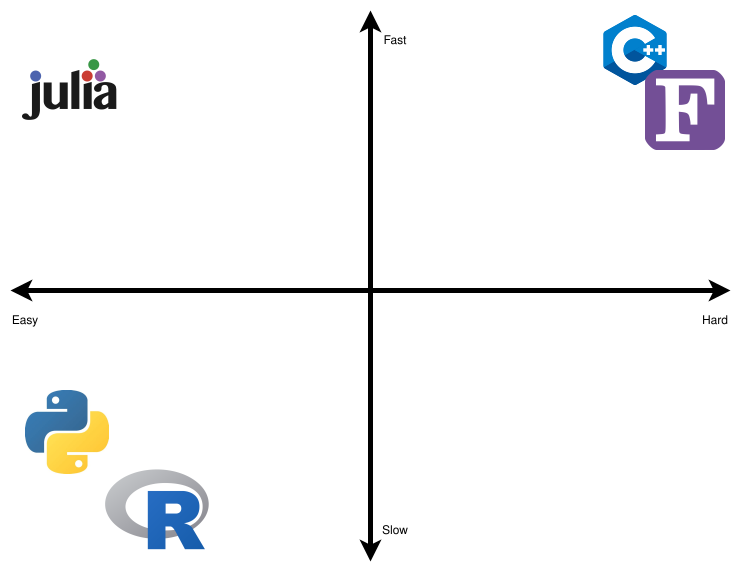
\includegraphics{images/language_comparisons.png}
\caption{科学计算编程语言比较:FORTRAN、C++、Python、R 和
Julia。}\label{fig:language_comparison}
}
\end{figure}

\textbf{Julia 很快! 特别快!} 它起初就为速度而设计。
而这通过多重派发实现。 基本上,这个想法能够生成非常高效的
LLVM\footnote{LLVM 是 \textbf{L}ow \textbf{L}evel \textbf{V}irtual
  \textbf{M}chine 的缩写,你可以在LLVM
  网站(\url{http://llvm.org})找到更多信息。} 代码。 LLVM 代码,也称为
LLVM 指令,它非常靠近底层,即非常接近计算机执行的实际操作。
所以,本质上, Julia 会将你可读性好的手写代码转换为 LLVM 机器码。虽然
LLVM 机器码对于人类来说很难阅读,但对于计算机来说很容易。
例如,如果你定义了一个接收单个参数的函数并向该函数传递整数,然后 Julia
会创建一个 \textbf{专门的} \passthrough{\lstinline!MethodInstance!}。
下次你再向该函数传递整数时,Julia 将会查找之前创建的
\passthrough{\lstinline!MethodInstance!},并引用其执行操作。
一个\textbf{很棒的} 技巧是,可以在调用函数的嵌套函数中使用它。
例如,如果向函数 \passthrough{\lstinline!f!} 传递了某些数据类型,而
\passthrough{\lstinline!f!} 又调用了函数
\passthrough{\lstinline!g!},同时传递给 \passthrough{\lstinline!g!}
的数据类型都是相同且已知的,那么生成函数 \passthrough{\lstinline!g!}
就会硬编码到 \passthrough{\lstinline!f!} 中! 这意味着 Julia
不再需要查找
\passthrough{\lstinline!MethodInstances!},此时代码就会运行地非常快。
此处需要权衡的是,在某些情况下,早期关于硬编码
\passthrough{\lstinline!MethodInstances!} 的假设可能是无效的。
然后需要重新创建硬编码的 \passthrough{\lstinline!MethodInstances!}。
因此,权衡也需包括花时间推断哪些能够硬编码,而哪些不能。
这也解释了为什么 Julia 代码在第一次执行前通常要花费较长的时间: Julia
在背后优化代码。

编译器接着做它最擅长的事情:优化机器码\footnote{如果你想了解更多关于
  Julia 如何设计的内容,你绝对需要看
  \protect\hyperlink{ref-bezanson2017julia}{Bezanson et al.}
  (\protect\hyperlink{ref-bezanson2017julia}{2017}) 。}。 你可以在 Julia
网站上找到 Julia 和其他语言的
\href{https://julialang.org/benchmarks/}{benchmarks} 。
图~\ref{fig:benchmarks} 取自于
\href{https://julialang.org/benchmarks/}{Julia 网站的 benchmarks
节\footnote{请注意上述的 Julia 结果不包含编译时间。}}。 如你所见, Julia
是\textbf{相当} 快的。

\begin{figure}
\hypertarget{fig:benchmarks}{%
\centering
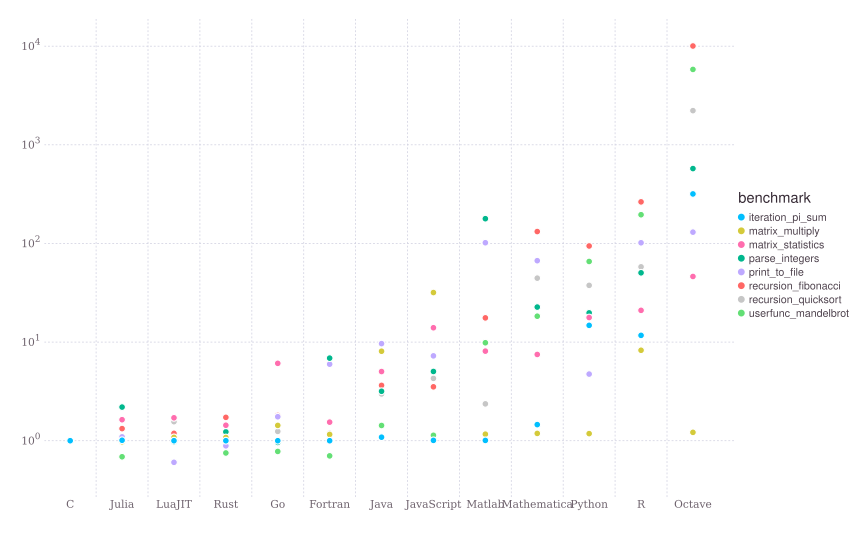
\includegraphics{images/benchmarks.png}
\caption{Julia VS 其他编程语言。}\label{fig:benchmarks}
}
\end{figure}

我们非常信任 Julia。 否则,我们不会写这本书。 我们认为, Julia 是
\textbf{科学计算和科学数据分析的未来}。
它使得用户可以通过简单的语法开发快速且强大的代码。
研究人员通常使用一种简单但缓慢的语言开发原型代码。
一旦确定代码正常运行且实现其目标,然后就会开始将当前的代码转换为一门快速但困难的编程语言。
这就是``两语言问题'',接下来将讨论它。

\hypertarget{sec:two_language}{%
\subsection{两语言问题}\label{sec:two_language}}

``两语言问题''
是科学计算中的典型问题。通常研究人员想要设计一种算法或方案来解决手头的问题或分析。
一般地,解决方案的原型代码都采用容易编程的语言(像 Python 或 R)。
如果原型能够正常工作,那么研究人员就会使用不易编写原型但快速的语言(C++
或 FORTRAN)重新实现。 因此,开发解决方案的过程涉及了两种语言。
一种语言易于编写原型代码并不适合方案实现 (通常由于缓慢的速度)。
而另一种语言并不易于编写原型代码,但由于非常快,所以适合方案实现。 Julia
能够避免此类情形,因为
\textbf{开发原型(易编程)和方案实现(速度快)将采用相同的语言}。

另外, Julia 允许使用 \textbf{Unicode 字符作为变量或参数}。
这意味着不再使用 \passthrough{\lstinline!sigma!} 或
\passthrough{\lstinline!sigma\_i!},而是像数学记号那样使用 \(σ\) 或
\(σᵢ\) 。 当查看算法代码或数学方程时,你会看到几乎相同的符号和术语。
我们将这种强大的特性称为 \textbf{``代码和数学关系的一对一''}。

我们认为,Alan Edelman,Julia
创始人之一,在一次\href{https://youtu.be/qGW0GT1rCvs}{TEDx Talk}
(\protect\hyperlink{ref-tedxtalksProgrammingLanguageHeal2020}{TEDx
Talks, 2020}) 中对 ``两语言问题'' 和 ``代码和数学关系的一对一''
作出了最好的描述。

\hypertarget{sec:multiple_dispatch}{%
\subsection{多重派发}\label{sec:multiple_dispatch}}

多重派发(multiple
dispatch)是一种强大的特性,它使得能够扩展现有的函数或为新类型自定义复杂行为。
假设想要定义两种 \passthrough{\lstinline!struct!} 来表示不同的动物:

\begin{lstlisting}[language=Julia]
abstract type Animal end
struct Fox <: Animal
    weight::Float64
end
struct Chicken <: Animal
    weight::Float64
end
\end{lstlisting}

这表明此处定义了动物类型 \passthrough{\lstinline!Fox!} 和
\passthrough{\lstinline!Chicken!}。 然后生成名为 Fiona 的
\passthrough{\lstinline!Fox!} 和名为 Big Bird 的
\passthrough{\lstinline!Chicken!}。

\begin{lstlisting}[language=Julia]
fiona = Fox(4.2)
big_bird = Chicken(2.9)
\end{lstlisting}

为了知道他们的重量之和,编写如下的函数:

\begin{lstlisting}[language=Julia]
combined_weight(A1::Animal, A2::Animal) = A1.weight + A2.weight
\end{lstlisting}

\begin{lstlisting}[language=Output]
combined_weight (generic function with 1 method)
\end{lstlisting}

然后还想知道它们能否相处得好。 采用条件语句实现:

\begin{lstlisting}[language=Julia]
function naive_trouble(A::Animal, B::Animal)
    if A isa Fox && B isa Chicken
        return true
    elseif A isa Chicken && B isa Fox
        return true
    elseif A isa Chicken && B isa Chicken
        return false
    end
end
\end{lstlisting}

\begin{lstlisting}[language=Output]
naive_trouble (generic function with 1 method)
\end{lstlisting}

现在,看看 Fiona 和 Big Bird 待在一起是否会产生麻烦:

\begin{lstlisting}[language=Julia]
naive_trouble(fiona, big_bird)
\end{lstlisting}

\begin{lstlisting}[language=Output]
true
\end{lstlisting}

好的,看起来不错。 编写 \passthrough{\lstinline!naive\_trouble!}
函数已经足够简单了。然而,使用多重派发编写
\passthrough{\lstinline!trouble!}
函数还可以带来新的优势。按照如下方式创建函数:

\begin{lstlisting}[language=Julia]
trouble(F::Fox, C::Chicken) = true
trouble(C::Chicken, F::Fox) = true
trouble(C1::Chicken, C2::Chicken) = false
\end{lstlisting}

\begin{lstlisting}[language=Output]
trouble (generic function with 3 methods)
\end{lstlisting}

定义这些方法后,\passthrough{\lstinline!trouble!} 会得到与
\passthrough{\lstinline!naive\_trouble!} 相同的结果。 例如:

\begin{lstlisting}[language=Julia]
trouble(fiona, big_bird)
\end{lstlisting}

\begin{lstlisting}[language=Output]
true
\end{lstlisting}

把 Big Bird 和另外一只小鸡 Dora 放在一起也是可以的。

\begin{lstlisting}[language=Julia]
dora = Chicken(2.2)
trouble(dora, big_bird)
\end{lstlisting}

\begin{lstlisting}[language=Output]
false
\end{lstlisting}

所以在本例中,多重派发的优势就是可以仅声明类型,然后由 Julia
去为类型找到正确的函数方法。
若是在嵌套函数中使用多重派发则更是如此,Julia
编译器实际上会自动优化函数调用。 例如,函数如下:

\begin{lstlisting}
function trouble(A::Fox, B::Chicken, C::Chicken)
    return trouble(A, B) || trouble(B, C) || trouble(C, A)
end
\end{lstlisting}

根据上下文,Julia 会将其优化为:

\begin{lstlisting}
function trouble(A::Fox, B::Chicken, C::Chicken)
    return true || false || true
end
\end{lstlisting}

因为编译器 \textbf{知道} \passthrough{\lstinline!A!} 是
\passthrough{\lstinline!Fox!}, \passthrough{\lstinline!B!} 是
\passthrough{\lstinline!Chicken!} ,所以方法替换为
\passthrough{\lstinline!trouble(F::Fox, C::Chicken)!}。
\passthrough{\lstinline!trouble(C1::Chicken, C2::Chicken)!} 同理。
然后,编译器进一步优化:

\begin{lstlisting}
function trouble(A::Fox, B::Chicken, C::Chicken)
    return true
end
\end{lstlisting}

此外,多重派发还使比较已存在的动物和新的动物 Zebra 成为可能。
可以在其他包中定义 Zebra :

\begin{lstlisting}[language=Julia]
struct Zebra <: Animal
    weight::Float64
end
\end{lstlisting}

然后定义与现有动物的交互:

\begin{lstlisting}[language=Julia]
trouble(F::Fox, Z::Zebra) = false
trouble(Z::Zebra, F::Fox) = false
trouble(C::Chicken, Z::Zebra) = false
trouble(Z::Zebra, F::Fox) = false
\end{lstlisting}

\begin{lstlisting}[language=Output]
trouble (generic function with 6 methods)
\end{lstlisting}

现在可查看 Marty(Zebra 动物)是否能与 Big Bird 和谐相处:

\begin{lstlisting}[language=Julia]
marty = Zebra(412)
trouble(big_bird, marty)
\end{lstlisting}

\begin{lstlisting}[language=Output]
false
\end{lstlisting}

更好的是,\textbf{不需额外定义任何函数即可计算 Zebra
和其他动物的重量之和}:

\begin{lstlisting}[language=Julia]
combined_weight(big_bird, marty)
\end{lstlisting}

\begin{lstlisting}[language=Output]
414.9
\end{lstlisting}

因此,总而言之,即使在编写代码时只考虑了 \passthrough{\lstinline!Fox!}
和 \passthrough{\lstinline!Chicken!},但它也能用于 \textbf{从未见过的}
类型! 在实践中,这意味着重用其他 Julia 项目的代码会非常容易。

如果你和我们一样对多重派发感到兴奋,那么可以了解下面这些深入的例子。
第一个例子是,\protect\hyperlink{ref-storopoli2021bayesianjulia}{Storopoli}
(\protect\hyperlink{ref-storopoli2021bayesianjulia}{2021}) 关于
\href{https://storopoli.io/Bayesian-Julia/pages/1_why_Julia/\#example_one-hot_vector}{one-hot
向量的快速而优雅的实现} 。
第二个例子是,\href{https://youtu.be/moyPIhvw4Nk?t=2107}{Tanmay Bakshi
YouTube 频道} 对 \href{https://www.chrisrackauckas.com/}{Christopher
Rackauckas} 的采访 (查看时间 35:07 )
(\protect\hyperlink{ref-tanmaybakshiBakingKnowledgeMachine2021}{tanmay
bakshi, 2021})。 Chris 提到, 在他开发和维护
\href{https://diffeq.sciml.ai/dev/}{\passthrough{\lstinline!DifferentialEquations.jl!}}
包时,一名用户报告问题说:他基于 GPU 构造的 ODE 求解器并不能正常工作。
Chris 对这个请求感到非常惊讶,因为他从来没有期望能够将 GPU
计算与求解边界值问题结合起来。
他甚至更惊讶地发现,用户犯了一个小错误,但一切正常。
这些大多数优点都来自于多重派发和高可用的代码 / 类型共享。

总的来说,我们认为多重派发的最好解释来自于 Julia 创始人
\href{https://youtu.be/kc9HwsxE1OY}{Stefan Karpinski 在 JuliaCon 2019
的演讲}。

\hypertarget{sec:julia_wild}{%
\section{Julia 应用案例}\label{sec:julia_wild}}

Section~\ref{sec:julia_accomplish} 解释了为什么我们认为 Julia
是门如此独一无二的编程语言。 我们在上节展示了一些 Julia 特性的简单例子。
如果想要深入了解 Julia 的使用, 下面介绍一些 \textbf{有趣的案例}:

\begin{enumerate}
\def\labelenumi{\arabic{enumi}.}
\tightlist
\item
  NASA 使用 Julia 在超级计算机上分析了
  \href{https://exoplanets.nasa.gov/news/1669/seven-rocky-trappist-1-planets-may-be-made-of-similar-stuff/}{``迄今为止发现的最大一批地球尺寸的行星''}
  ,并且实现了惊人的 \textbf{1,000 倍加速},在 15 分钟内分类了1.88
  亿个天体。
\item
  \href{https://clima.caltech.edu/}{气候建模联盟(Climate Modeling
  Alliance,CliMa)} \textbf{在 GPU 和 CPU 上模拟天气}。 该项目启动于
  2018 年,与加州理工大学、 NASA
  喷气推进实验室以及海军研究生院的研究人员合作,CliMa
  项目组采用最近的计算科学进展来开发一个地球系统模型,该模型能够以前所未有的精度和速度预测干旱、热浪和降雨。
\item
  \href{https://youtu.be/19zm1Fn0S9M}{美国联邦航空管理局 (FAA) 正在使用
  Julia 开发一种 \textbf{空中防碰撞系统 (ACAS-X)}}。
  这也是一个``两语言问题'' 的好例子(查看
  Section~\ref{sec:julia_accomplish})。 之前的方案是使用 Matlab
  开发算法 并使用 C++ 编写高性能实现。 现在,FAA 使用 Julia
  语言完成所有的事。
\item
  \href{https://juliacomputing.com/case-studies/pfizer/}{使用 Julia 在
  GPU 上 \textbf{175 倍加速} 辉瑞的药理学模型}。
  这是一份第11届美国定量药理学会议的\href{https://chrisrackauckas.com/assets/Posters/ACoP11_Poster_Abstracts_2020.pdf}{海报},它还获得了
  \href{https://web.archive.org/web/20210121164011/https://www.go-acop.org/abstract-awards}{quality
  award}。
\item
  \href{https://discourse.julialang.org/t/julia-and-the-satellite-amazonia-1/57541}{巴西卫星亚马逊
  1 号的姿态和轨道控制子系统 (AOCS) \textbf{100\% 使用 Julia 编写}}
  ,它的作者是 Ronan Arraes Jardim Chagas
  (\url{https://ronanarraes.com/})。
\item
  \href{https://youtu.be/NY0HcGqHj3g}{巴西国家发展银行 (BNDES)
  放弃了付费解决方案,转而选择开源 Julia 模型并获得 \textbf{10
  倍加速}。}
\end{enumerate}

如果觉得这些仍不够,\href{https://juliacomputing.com/case-studies/}{Julia
计算网站} 上还有更多的例子。

\hypertarget{sec:julia_basics}{%
\chapter{Julia 基础}\label{sec:julia_basics}}

\begin{quote}
\textbf{\emph{NOTE:}} 本章介绍 Julia 编程语言的基础。 请注意,使用 Julia
语言作为数据分析和数据可视化工具不是 \textbf{严格必须} 的。 了解 Julia
的基础知识可以让你更加 \textbf{有效} 且 \textbf{高效} 地使用 Julia 。
但是,如果希望直接开始,可以跳转到 Section~\ref{sec:dataframes}
,学习使用 \passthrough{\lstinline!DataFrames.jl!} 操作表格数据。
\end{quote}

本章是对 Julia 语言的简要概述。
如果您已经熟悉其他编程语言,我们强烈建议您阅读 Julia 文档
(\url{https://docs.julialang.org/})。 Julia 文档是深入理解 Julia
的绝佳资源。
它包含了所有的基础和特殊案例,但在你并不熟悉软件文档时会变得很复杂。

接下来将介绍 Julia 的基本知识。 想象一下,若把Julia
比作一辆功能丰富的奇特汽车,比如一辆全新的特斯拉,那么本章只会向您介绍如何``驾驶汽车、停车和在道路上导航''。
若你想知道``方向盘和仪表盘上的所有按钮的作用'',那本章不是您要找的资源。

\hypertarget{sec:ide}{%
\section{开发环境}\label{sec:ide}}

在深入研究语法前,我们需要了解如何运行代码。
详细介绍各种运行方案超出本书讨论的范围。因此,本节只对每种方案作简要介绍。

最简单的方案是使用 Julia REPL。 这指的是启动 Julia 可执行文件
(\passthrough{\lstinline!julia!} or \passthrough{\lstinline!julia.exe!})
并且在其中运行代码。 例如,启动 REPL 并执行一些代码:

\begin{lstlisting}
julia> x = 2
2

julia> x + 1
3
\end{lstlisting}

代码都运行正常,但是如果我们想保存编写的代码,该怎么办?
我们可以通过编写 ``.jl'' 文件来保存代码,例如 ``script.jl''
,并将它加载到 Julia 中。 ``script.jl'' 包含:

\begin{lstlisting}
x = 3
y = 4
\end{lstlisting}

将它加载到 Julia:

\begin{lstlisting}
julia> include("script.jl")

julia> y
4
\end{lstlisting}

现在的问题是,如何使 Julia 在每次执行代码前重新读取我们的脚本。
\href{https://github.com/timholy/Revise.jl}{Revise.jl} 实现了这一功能。
因为 Julia 中的编译时间通常很长,所以
\passthrough{\lstinline!Revise.jl!} 是 Julia 开发的必备工具。
有关更多信息,请阅读 \passthrough{\lstinline!Revise.jl!} 文档或者在
Google 上搜索具体的问题。

我们还发现 \passthrough{\lstinline!Revise.jl!} 和 REPL
需要一些手动操作,但文档并没有将这些操作写清楚。 幸运的是,还有
\href{https://github.com/fonsp/Pluto.jl}{Pluto.jl}。
\passthrough{\lstinline!Pluto.jl!} 能够自动管理依赖, 运行代码, 和
\textbf{交互式} 地更改代码。 对于刚接触编程的人来说,
\passthrough{\lstinline!Pluto.jl!} 是最简单的入门方案。
此软件包的主要缺点是不够适合大型项目。

一些其他选项是使用安装了多种 Julia 插件 的 Visual Studio Code
或定制你自己的 IDE。 如果你 \textbf{不知道} 什么是
IDE,但又想管理大型项目,请选择 Visual Studio Code 。 如果你
\textbf{知道} 什么是 IDE,那你可以使用 Vim 或者Emacs 结合 REPL
来构建自己的 IDE。

综上所述:

\begin{itemize}
\tightlist
\item
  最简单的入门方案 -\textgreater{} \passthrough{\lstinline!Pluto.jl!}
\item
  大型项目 -\textgreater{} Visual Studio Code
\item
  高级用户 -\textgreater{} Vim, Emacs and the REPL
\end{itemize}

\hypertarget{sec:syntax}{%
\section{语法}\label{sec:syntax}}

Julia 是一种即时编译的\textbf{动态类型语言}。 这意味着不像 C++ 或
FORTRAN 那样,需要在运行之前编译程序。 相反,Julia
会读取你的代码,并在运行前编译部分程序。
同时,你不需要为每一处代码显式地指定类型,Julia会在运行时推断类型。

Julia 与其他动态语言(如 R 和 Python)之间的主要区别如下。 首先,Julia
\textbf{允许用户进行类型声明} 。你应该在 \textbf{为什么选择 Julia?}
(Section~\ref{sec:why_julia}):
一节已经见过类型声明,就是一些跟在变量后的双冒号
\passthrough{\lstinline!::!} 。
但是,如果你不想指定变量或函数的类型,Julia 将会很乐意推断(猜测)它们。

其次,Julia 允许用户通过多重派发定义不同参数类型组合的函数行为。
本书将会在 Section~\ref{sec:julia_accomplish} 讨论多重派发。
定义不同函数行为的方法是使用相同的函数名称定义新的函数,但将这些函数用于不同的参数类型。

\hypertarget{sec:variable}{%
\subsection{变量}\label{sec:variable}}

变量是在计算机中以特定名称存储的值,以便后面读取或更改此值。 Julia
有很多数据类型,但在数据科学中主要使用:

\begin{itemize}
\tightlist
\item
  整数: \passthrough{\lstinline!Int64!}
\item
  实数: \passthrough{\lstinline!Float64!}
\item
  布尔型: \passthrough{\lstinline!Bool!}
\item
  字符串: \passthrough{\lstinline!String!}
\end{itemize}

整数和实数默认使用 64 位存储,这就是为什么它们的类型名称带有``64''后缀。
如果需要更高或更低的精度,Julia 还有 \passthrough{\lstinline!Int8!}
类型和 \passthrough{\lstinline!Int128!} 类型,其中
\passthrough{\lstinline!Int8!}
类型用于低精度,\passthrough{\lstinline!Int128!} 类型用于高精度。
多数情况下,用户不需要关心精度问题,使用默认值即可。

创建新变量的方法是在左侧写变量名并在右侧写其值,并在中间插入\passthrough{\lstinline!=!}
赋值运算符。 例如:

\begin{lstlisting}[language=Julia]
name = "Julia"
age = 9
\end{lstlisting}

\begin{lstlisting}[language=Output]
9
\end{lstlisting}

请注意,最后一行代码 (\passthrough{\lstinline!age!})
的值已打印到控制台。 上面的代码定义了两个变量
\passthrough{\lstinline!name!} 和 \passthrough{\lstinline!age!}。
将变量名称输入可重新得到变量的值:

\begin{lstlisting}[language=Julia]
name
\end{lstlisting}

\begin{lstlisting}[language=Output]
Julia
\end{lstlisting}

如果要为现有变量定义新值,可以重复赋值中的步骤。 请注意,Julia
现在将使用新值覆盖旧值。 假设 Julia 已经过了生日,现在是 10 岁:

\begin{lstlisting}[language=Julia]
age = 10
\end{lstlisting}

\begin{lstlisting}[language=Output]
10
\end{lstlisting}

我们可以对 \passthrough{\lstinline!name!} 进行同样的操作。假设 Julia
因为惊人的速度获得了一些头衔。那么,我们可以更改
\passthrough{\lstinline!name!} 的值:

\begin{lstlisting}[language=Julia]
name = "Julia Rapidus"
\end{lstlisting}

\begin{lstlisting}[language=Output]
Julia Rapidus
\end{lstlisting}

也可以对变量进行乘除法等运算。 将 \passthrough{\lstinline!age!} 乘以
12,可以得到 Julia 以月为单位的年龄:

\begin{lstlisting}[language=Julia]
12 * age
\end{lstlisting}

\begin{lstlisting}[language=Output]
120
\end{lstlisting}

使用 \passthrough{\lstinline!typeof!} 函数可以查看变量的类型:

\begin{lstlisting}[language=Julia]
typeof(age)
\end{lstlisting}

\begin{lstlisting}[language=Output]
Int64
\end{lstlisting}

接下来的问题是:``我还能对整数做什么?'' Julia 中 有一个非常好用的函数
\passthrough{\lstinline!methodswith!}
,它可以为输出所有可用于指定类型的函数。 此处限制代码只显示前五行:

\begin{lstlisting}[language=Julia]
first(methodswith(Int64), 5)
\end{lstlisting}

\begin{lstlisting}[language=Output]
[1] logmvbeta(p::Int64, a::T, b::T) where T<:Real in StatsFuns at /home/runner/.julia/packages/StatsFuns/mQJB7/src/misc.jl:22
[2] logmvbeta(p::Int64, a::Real, b::Real) in StatsFuns at /home/runner/.julia/packages/StatsFuns/mQJB7/src/misc.jl:23
[3] logmvgamma(p::Int64, a::Real) in StatsFuns at /home/runner/.julia/packages/StatsFuns/mQJB7/src/misc.jl:8
[4] read(t::HTTP.ConnectionPool.Transaction, nb::Int64) in HTTP.ConnectionPool at /home/runner/.julia/packages/HTTP/aTjcj/src/ConnectionPool.jl:232
[5] write(ctx::MbedTLS.MD, i::Union{Float16, Float32, Float64, Int128, Int16, Int32, Int64, UInt128, UInt16, UInt32, UInt64}) in MbedTLS at /home/runner/.julia/packages/MbedTLS/Vaaz8/src/md.jl:140
\end{lstlisting}

\hypertarget{sec:struct}{%
\subsection{用户定义类型}\label{sec:struct}}

不凭借任何依赖关系或层次结构来组织多个变量是不现实的。 在 Julia
中,我们可以使用
\passthrough{\lstinline!struct!}(也称为复合类型)来定义结构化数据。
在每个 \passthrough{\lstinline!struct!} 中都可以定义一组字段。
它们不同于 Julia 语言内核中已经默认定义的原始类型(例如
\passthrough{\lstinline!Integer!} 和 \passthrough{\lstinline!Float!})。
由于大多数 \passthrough{\lstinline!struct!}
都是用户定义的,因此它们也被称为用户定义类型。

例如,创建 \passthrough{\lstinline!struct!}
表示用于科学计算的开源编程语言。 在 \passthrough{\lstinline!struct!}
中定义一组相应类型的字段:

\begin{lstlisting}[language=Julia]
struct Language
    name::String
    title::String
    year_of_birth::Int64
    fast::Bool
end
\end{lstlisting}

可以通过将 \passthrough{\lstinline!struct!} 作为参数传递给
\passthrough{\lstinline!fieldnames!}检查字段名称列表:

\begin{lstlisting}[language=Julia]
fieldnames(Language)
\end{lstlisting}

\begin{lstlisting}[language=Output]
(:name, :title, :year_of_birth, :fast)
\end{lstlisting}

要使用
\passthrough{\lstinline!struct!},必须创建单个实例(或``对象''),每个\passthrough{\lstinline!struct!}实例的字段值都是特定的。
如下所示,创建两个实例 Julia 和 Python:

\begin{lstlisting}[language=Julia]
julia = Language("Julia", "Rapidus", 2012, true)
python = Language("Python", "Letargicus", 1991, false)
\end{lstlisting}

\begin{lstlisting}[language=Output]
Language("Python", "Letargicus", 1991, false)
\end{lstlisting}

\passthrough{\lstinline!struct!} 实例的值在构造后无法修改。
如果需要,可以创建 \passthrough{\lstinline!mutable struct!}。
但请注意,可变对象一般来说更慢且更容易出现错误。
因此,尽可能确保所有类型都是 \textbf{不可变的}。 接下来创建一个
\passthrough{\lstinline!mutable struct!}:

\begin{lstlisting}[language=Julia]
mutable struct MutableLanguage
    name::String
    title::String
    year_of_birth::Int64
    fast::Bool
end

julia_mutable = MutableLanguage("Julia", "Rapidus", 2012, true)
\end{lstlisting}

\begin{lstlisting}[language=Output]
MutableLanguage("Julia", "Rapidus", 2012, true)
\end{lstlisting}

假设想要改变 \passthrough{\lstinline!julia\_mutable!} 的标题。 因为
\passthrough{\lstinline!julia\_mutable!} 是
\passthrough{\lstinline!mutable struct!} 的实例,所以该操作可行:

\begin{lstlisting}[language=Julia]
julia_mutable.title = "Python Obliteratus"

julia_mutable
\end{lstlisting}

\begin{lstlisting}[language=Output]
MutableLanguage("Julia", "Python Obliteratus", 2012, true)
\end{lstlisting}

\hypertarget{ux5e03ux5c14ux8fd0ux7b97ux548cux6570ux503cux6bd4ux8f83}{%
\subsection{布尔运算和数值比较}\label{ux5e03ux5c14ux8fd0ux7b97ux548cux6570ux503cux6bd4ux8f83}}

上节讨论了类型,本节讨论布尔运算和数值比较。

Julia 中有三种布尔运算符:

\begin{itemize}
\tightlist
\item
  \passthrough{\lstinline"!"} ~: \textbf{NOT}
\item
  \passthrough{\lstinline!\&\&!}: \textbf{AND}
\item
  \passthrough{\lstinline!||!}: \textbf{OR}
\end{itemize}

一些例子如下:

\begin{lstlisting}[language=Julia]
!true
\end{lstlisting}

\begin{lstlisting}[language=Output]
false
\end{lstlisting}

\begin{lstlisting}[language=Julia]
(false && true) || (!false)
\end{lstlisting}

\begin{lstlisting}[language=Output]
true
\end{lstlisting}

\begin{lstlisting}[language=Julia]
(6 isa Int64) && (6 isa Real)
\end{lstlisting}

\begin{lstlisting}[language=Output]
true
\end{lstlisting}

关于数值比较,Julia有三种主要的比较类型:

\begin{enumerate}
\def\labelenumi{\arabic{enumi}.}
\tightlist
\item
  \textbf{相等}:两者的关系为 \textbf{相等} 或 \textbf{不等}

  \begin{itemize}
  \tightlist
  \item
    == ``相等''
  \item
    != 或 ≠ ``不等''
  \end{itemize}
\item
  \textbf{小于}: 两者的关系为 \textbf{小于} 或 \textbf{小于等于}

  \begin{itemize}
  \tightlist
  \item
    \textless{} ``小于''
  \item
    \textless= 或 ≤ ``小于等于''
  \end{itemize}
\item
  \textbf{大于}: 两者的关系为 \textbf{大于} 或 \textbf{大于等于}

  \begin{itemize}
  \tightlist
  \item
    \textgreater{} ``大于''
  \item
    \textgreater= 或 ≥ ``大于等于''
  \end{itemize}
\end{enumerate}

下面是一些例子:

\begin{lstlisting}[language=Julia]
1 == 1
\end{lstlisting}

\begin{lstlisting}[language=Output]
true
\end{lstlisting}

\begin{lstlisting}[language=Julia]
1 >= 10
\end{lstlisting}

\begin{lstlisting}[language=Output]
false
\end{lstlisting}

甚至可以比较不同类型:

\begin{lstlisting}[language=Julia]
1 == 1.0
\end{lstlisting}

\begin{lstlisting}[language=Output]
true
\end{lstlisting}

还可以将布尔运算与数值比较:

\begin{lstlisting}[language=Julia]
(1 != 10) || (3.14 <= 2.71)
\end{lstlisting}

\begin{lstlisting}[language=Output]
true
\end{lstlisting}

\hypertarget{sec:function}{%
\subsection{函数}\label{sec:function}}

上节学习了如何定义变量和自定义类型
\passthrough{\lstinline!struct!},本节讨论 \textbf{函数}。 在 Julia
里,函数是 \textbf{一组参数值到一个或多个返回值的映射}。
基础语法如下所示:

\begin{lstlisting}
function function_name(arg1, arg2)
    result = stuff with the arg1 and arg2
    return result
end
\end{lstlisting}

函数声明以关键字 \passthrough{\lstinline!function!} 开始,后接函数名称。
然后在 \passthrough{\lstinline!()!} 里定义参数, 这些参数由
\passthrough{\lstinline!,!} 分隔。 接着在函数体内部定义我们希望 Julia
对传入参数执行的操作。
函数里定义的所有变量都会在函数返回后删除。这很不错,因为有点像自动垃圾回收。
在函数体内的所有操作完成后,Julia 使用 \passthrough{\lstinline!return!}
关键字返回最终结果。 最后,Julia 以 \passthrough{\lstinline!end!}
关键字结束函数定义。

还有一种紧凑的 \textbf{赋值形式}:

\begin{lstlisting}
f_name(arg1, arg2) = stuff with the arg1 and arg2
\end{lstlisting}

这种形式更加紧凑,但 \textbf{等效于} 前面的同名函数。
根据经验,当代码符合一行最多只有92字符时,紧凑形式更加合适。
否则,只需使用带 \passthrough{\lstinline!function!} 关键字的较长形式。
接下来深入讨论一些例子。

\hypertarget{sec:function_example}{%
\subsubsection{创建函数}\label{sec:function_example}}

下面是一个将传入数字相加的函数:

\begin{lstlisting}[language=Julia]
function add_numbers(x, y)
    return x + y
end
\end{lstlisting}

\begin{lstlisting}[language=Output]
add_numbers (generic function with 1 method)
\end{lstlisting}

接下来调用 \passthrough{\lstinline!add\_numbers!} 函数:

\begin{lstlisting}[language=Julia]
add_numbers(17, 29)
\end{lstlisting}

\begin{lstlisting}[language=Output]
46
\end{lstlisting}

它也适用于浮点数:

\begin{lstlisting}[language=Julia]
add_numbers(3.14, 2.72)
\end{lstlisting}

\begin{lstlisting}[language=Output]
5.86
\end{lstlisting}

另外,还可以通过制定类型声明来创建自定义函数行为。 假设创建一个
\passthrough{\lstinline!round\_number!} 函数, 它在传入参数类型是
\passthrough{\lstinline!Float64!} 或 \passthrough{\lstinline!Int64!}
时进行不同的操作:

\begin{lstlisting}[language=Julia]
function round_number(x::Float64)
    return round(x)
end

function round_number(x::Int64)
    return x
end
\end{lstlisting}

\begin{lstlisting}[language=Output]
round_number (generic function with 2 methods)
\end{lstlisting}

可以看到,它是具有多种方法的函数:

\begin{lstlisting}[language=Julia]
methods(round_number)
\end{lstlisting}

\begin{lstlisting}[language=Output]
round_number(x::Float64) in Main at none:1
\end{lstlisting}

\begin{lstlisting}[language=Output]
round_number(x::Int64) in Main at none:5
\end{lstlisting}

但问题是:如果想对 32 位浮点数 \passthrough{\lstinline!Float32!} 或者 8
位整数 \passthrough{\lstinline!Int8!} 作四舍五入,该怎么办?

如果想定义关于所有浮点数和整数类型的函数,那么需要使用 \textbf{abstract
type} 作为函数签名, 例如 \passthrough{\lstinline!AbstractFloat!} 或
\passthrough{\lstinline!Integer!}:

\begin{lstlisting}[language=Julia]
function round_number(x::AbstractFloat)
    return round(x)
end
\end{lstlisting}

\begin{lstlisting}[language=Output]
round_number (generic function with 3 methods)
\end{lstlisting}

现在该函数适用于任何的浮点数类型:

\begin{lstlisting}[language=Julia]
x_32 = Float32(1.1)
round_number(x_32)
\end{lstlisting}

\begin{lstlisting}[language=Output]
1.0f0
\end{lstlisting}

\begin{quote}
\textbf{\emph{NOTE:}} 可以使用 \passthrough{\lstinline!supertypes!} 和
\passthrough{\lstinline!subtypes!} 函数查看类型间的关系。
\end{quote}

接下来回到之前定义的 \passthrough{\lstinline!Language!}
\passthrough{\lstinline!struct!}。 这就是一个多重派发的例子。 下面将扩展
\passthrough{\lstinline!Base.show!} 函数,该函数打印实例的类型和
\passthrough{\lstinline!struct!} 的内容。

默认情况下, \passthrough{\lstinline!struct!} 有基本的输出样式,正如在
\passthrough{\lstinline!python!} 例子中看到的那样。 可以为
\passthrough{\lstinline!Language!} 类型定义新的
\passthrough{\lstinline!Base.show!} 方法,
以便为编程语言实例提供更漂亮的输出。
该方法将更清晰地打印编程语言的姓名,称号和年龄。 函数
\passthrough{\lstinline!Base.show!} 接收两个参数,第一个是
\passthrough{\lstinline!IO!} 类型的 \passthrough{\lstinline!io!}
,另一个是 \passthrough{\lstinline!Language!} 类型的
\passthrough{\lstinline!l!}:

\begin{lstlisting}[language=Julia]
Base.show(io::IO, l::Language) = print(
    io, l.name, ", ",
    2021 - l.year_of_birth, " years old, ",
    "has the following titles: ", l.title
)
\end{lstlisting}

现在查看 \passthrough{\lstinline!python!} 如何输出:

\begin{lstlisting}[language=Julia]
python
\end{lstlisting}

\begin{lstlisting}[language=Output]
Python, 30 years old, has the following titles: Letargicus
\end{lstlisting}

\hypertarget{sec:function_multiple}{%
\subsubsection{多返回值}\label{sec:function_multiple}}

一个函数可以返回两个以上的值。 下面看一个新函数
\passthrough{\lstinline!add\_multiply!}:

\begin{lstlisting}[language=Julia]
function add_multiply(x, y)
    addition = x + y
    multiplication = x * y
    return addition, multiplication
end
\end{lstlisting}

\begin{lstlisting}[language=Output]
add_multiply (generic function with 1 method)
\end{lstlisting}

再接收返回值时,有两种写法:

\begin{enumerate}
\def\labelenumi{\arabic{enumi}.}
\item
  与返回值的形式类似,依次为每个返回值定义一个变量,在本例中则需要两个变量:

  \begin{lstlisting}[language=Julia]
  return_1, return_2 = add_multiply(1, 2)
  return_2
  \end{lstlisting}

  \begin{lstlisting}[language=Output]
  2
  \end{lstlisting}
\item
  也可以定义一个变量来接受所有的返回值,然后通过
  \passthrough{\lstinline!first!} 或 \passthrough{\lstinline!last!}
  访问每个返回值:

  \begin{lstlisting}[language=Julia]
  all_returns = add_multiply(1, 2)
  last(all_returns)
  \end{lstlisting}

  \begin{lstlisting}[language=Output]
  2
  \end{lstlisting}
\end{enumerate}

\hypertarget{sec:function_keyword_arguments}{%
\subsubsection{关键字参数}\label{sec:function_keyword_arguments}}

某些函数可以接受关键字参数而不是位置参数。
这些参数与常规参数类似,只是定义在常规函数参数之后且使用分号
\passthrough{\lstinline!;!} 分隔。 例如,定义
\passthrough{\lstinline!logarithm!} 函数,该函数默认使用基 \(e\)
(2.718281828459045)作为关键字参数。 注意,此处使用抽象类型
\passthrough{\lstinline!Real!},以便于覆盖从
\passthrough{\lstinline!Integer!} 和
\passthrough{\lstinline!AbstractFloat!}
派生的所有类型,这两种类型本身也都是 \passthrough{\lstinline!Real!}
的子类型:

\begin{lstlisting}[language=Julia]
AbstractFloat <: Real && Integer <: Real
\end{lstlisting}

\begin{lstlisting}[language=Output]
true
\end{lstlisting}

\begin{lstlisting}[language=Julia]
function logarithm(x::Real; base::Real=2.7182818284590)
    return log(base, x)
end
\end{lstlisting}

\begin{lstlisting}[language=Output]
logarithm (generic function with 1 method)
\end{lstlisting}

当未指定 \passthrough{\lstinline!base!}
参数时函数正常运行,这是因为函数声明中提供了 \textbf{默认参数} :

\begin{lstlisting}[language=Julia]
logarithm(10)
\end{lstlisting}

\begin{lstlisting}[language=Output]
2.3025850929940845
\end{lstlisting}

同时也可以指定与默认值不同的 \passthrough{\lstinline!base!} 值:

\begin{lstlisting}[language=Julia]
logarithm(10; base=2)
\end{lstlisting}

\begin{lstlisting}[language=Output]
3.3219280948873626
\end{lstlisting}

\hypertarget{sec:function_anonymous}{%
\subsubsection{匿名函数}\label{sec:function_anonymous}}

很多情况下,我们不关心函数名称,只想快速创建函数。 因此我们需要
\textbf{匿名函数} 。 Julia 数据科学工作流中经常会用到它。 例如,在使用
\passthrough{\lstinline!DataFrames.jl!} (Section~\ref{sec:dataframes})
或 \passthrough{\lstinline!Makie.jl!}
(Section~\ref{sec:DataVisualizationMakie})
时,时常需要一个临时函数来筛选数据或者格式化图标签。
这就是使用匿名函数的时机。
当我们不想创建函数时它特别有用,因为一个简单的 in-place 语句就够用了。

它的语法特别简单, 只需使用 \passthrough{\lstinline!->!} 。
\passthrough{\lstinline!->!} 的左侧定义参数名称。
\passthrough{\lstinline!->!} 的右侧定义了想对左侧参数进行的操作。
考虑这样一个例子, 假设想通过指数函数来抵消对数运算:

\begin{lstlisting}[language=Julia]
map(x -> 2.7182818284590^x, logarithm(2))
\end{lstlisting}

\begin{lstlisting}[language=Output]
2.0
\end{lstlisting}

这里使用 \passthrough{\lstinline!map!}
函数方便地将匿名函数(第一个参数)映射到了
\passthrough{\lstinline!logarithm(2)!} (第二个参数)。
因此,我们得到了相同的数字,因为指数运算和对数运算是互逆的(在选择相同的基
-- 2.7182818284590 时)。

\hypertarget{sec:conditionals}{%
\subsection{条件表达式 If-Elseif-Else}\label{sec:conditionals}}

在大多数语言中,用户可以控制程序的执行流。
我们可依据情况使计算机做这一件或另外一件事。 Julia 使用
\passthrough{\lstinline!if!},\passthrough{\lstinline!elseif!} 和
\passthrough{\lstinline!else!} 关键字进行流程控制。
它们也被称为条件语句。

\passthrough{\lstinline!if!}
关键字执行一个表达式,,然后根据表达式的结果为
\passthrough{\lstinline!true!} 还是 \passthrough{\lstinline!false!}
执行相应分支的代码。 在复杂的控制流中,可以使用
\passthrough{\lstinline!elseif!} 组合多个 \passthrough{\lstinline!if!}
条件。 最后,如果 \passthrough{\lstinline!if!} 或
\passthrough{\lstinline!elseif!} 分支的语句都被执行为
\passthrough{\lstinline!true!},那么我们可以定义另外的分支。 这就是
\passthrough{\lstinline!else!} 关键字的作用。
与之前见到的关键字运算符一样,我们必须告诉 Julia 条件语句以
\passthrough{\lstinline!end!} 关键字结束。

下面是一个包含所有
\passthrough{\lstinline!if!}-\passthrough{\lstinline!elseif!}-\passthrough{\lstinline!else!}
关键字的例子:

\begin{lstlisting}[language=Julia]
a = 1
b = 2

if a < b
    "a is less than b"
elseif a > b
    "a is greater than b"
else
    "a is equal to b"
end
\end{lstlisting}

\begin{lstlisting}[language=Output]
a is less than b
\end{lstlisting}

我们甚至可将其包装成函数 \passthrough{\lstinline!compare!}:

\begin{lstlisting}[language=Julia]
function compare(a, b)
    if a < b
        "a is less than b"
    elseif a > b
        "a is greater than b"
    else
        "a is equal to b"
    end
end

compare(3.14, 3.14)
\end{lstlisting}

a is equal to b

\hypertarget{sec:for}{%
\subsection{For 循环}\label{sec:for}}

Julia 中的经典 for 循环遵循与条件语句类似的语法。 它以
\passthrough{\lstinline!for!} 关键字开始。 然后,向 Julia 指定一组要
``循环'' 的语句。 另外,与其他一样,它也以 \passthrough{\lstinline!end!}
关键字结束。

比如使用如下的 for 循环使 Julia 打印 1-10 的数字:

\begin{lstlisting}[language=Julia]
for i in 1:10
    println(i)
end
\end{lstlisting}

\hypertarget{sec:while}{%
\subsection{while 循环}\label{sec:while}}

while 循环是前面的条件语句和 for 循环的结合体。 在 while
循环中,当条件为 \passthrough{\lstinline!true!} 时将一直执行循环体。
语法与之前的语句相同。 以 \passthrough{\lstinline!while!}
开始,紧跟计算结果为 \passthrough{\lstinline!true!} 或
\passthrough{\lstinline!false!} 的条件表达式。 它仍以
\passthrough{\lstinline!end!} 关键字结束。

例子如下:

\begin{lstlisting}[language=Julia]
n = 0

while n < 3
    global n += 1
end

n
\end{lstlisting}

\begin{lstlisting}[language=Output]
3
\end{lstlisting}

可以看到,我们不得不使用 \passthrough{\lstinline!global!} 关键字。
这是因为, 在条件语句中,循环和函数内定义的变量仅存在于其内部。
这就是变量的 \textbf{作用域} 。 我们需要通过
\passthrough{\lstinline!global!} 关键字告诉 Julia
\passthrough{\lstinline!while!} 循环中的 \passthrough{\lstinline!n!}
是全局作用域中的 \passthrough{\lstinline!n!}。 最后,循环体使用的
\passthrough{\lstinline!+=!} 运算符是
\passthrough{\lstinline!n = n + 1!} 的缩写。

\hypertarget{sec:data_structures}{%
\section{原生数据结构}\label{sec:data_structures}}

Julia 有多种原生数据结构。 它们都是某种结构化数据形式的抽象。
本书将讨论最常用的数据结构。 它们都能够保存同类型或异构的数据。
因为它们都是集合, 所以都能通过 \passthrough{\lstinline!for!} 循环进行
\textbf{遍历} 。 接下来的讨论包括 \passthrough{\lstinline!String!},
\passthrough{\lstinline!Tuple!}, \passthrough{\lstinline!NamedTuple!},
\passthrough{\lstinline!UnitRange!}, \passthrough{\lstinline!Arrays!},
\passthrough{\lstinline!Pair!}, \passthrough{\lstinline!Dict!},
\passthrough{\lstinline!Symbol!}。

当在 Julia 中偶然发现某种数据结构时,可以使用
\passthrough{\lstinline!methodswith!}
函数查看能接收该数据结构作为参数的方法。 Julia 中方法和函数的区别如下。
如前面讨论的那样,每一个函数对应多种方法。 因此值得将
\passthrough{\lstinline!methodswith!} 函数收藏到你的技巧包里。
例如,让我们看看当对 \passthrough{\lstinline!String!}
应用该函数时会发生什么:

\begin{lstlisting}[language=Julia]
first(methodswith(String), 5)
\end{lstlisting}

\begin{lstlisting}[language=Output]
[1] write(fp::FilePathsBase.SystemPath, x::Union{String, Vector{UInt8}}) in FilePathsBase at /home/runner/.julia/packages/FilePathsBase/4RrDh/src/system.jl:380
[2] write(fp::FilePathsBase.SystemPath, x::Union{String, Vector{UInt8}}, mode) in FilePathsBase at /home/runner/.julia/packages/FilePathsBase/4RrDh/src/system.jl:380
[3] write(iod::HTTP.DebugRequest.IODebug, x::String) in HTTP.DebugRequest at /home/runner/.julia/packages/HTTP/aTjcj/src/IODebug.jl:38
[4] write(buffer::FilePathsBase.FileBuffer, x::String) in FilePathsBase at /home/runner/.julia/packages/FilePathsBase/4RrDh/src/buffer.jl:85
[5] write(io::IO, s::Union{SubString{String}, String}) in Base at strings/io.jl:244
\end{lstlisting}

\hypertarget{sec:broadcasting}{%
\subsection{对运算符和函数进行广播}\label{sec:broadcasting}}

在深入研究数据结构前,我们需要先讨论广播(也被称为 \textbf{向量化})和
\passthrough{\lstinline!.!} 点运算符。

可以使用点运算符广播像 \passthrough{\lstinline!*!} (乘)或
\passthrough{\lstinline!+!}(加)这样的数学运算。 例如,添加广播只需将
\passthrough{\lstinline!+!} 改为 \passthrough{\lstinline!.+!}:

\begin{lstlisting}[language=Julia]
[1, 2, 3] .+ 1
\end{lstlisting}

\begin{lstlisting}[language=Output]
[2, 3, 4]
\end{lstlisting}

函数也能通过这种操作实现广播。
(技术上讲,数学运算或中缀运算符也是函数,但这不重要。) 还记得
\passthrough{\lstinline!logarithm!} 函数吗?

\begin{lstlisting}[language=Julia]
logarithm.([1, 2, 3])
\end{lstlisting}

\begin{lstlisting}[language=Output]
[0.0, 0.6931471805599569, 1.0986122886681282]
\end{lstlisting}

\hypertarget{sec:function_bang}{%
\subsection{\texorpdfstring{带感叹号 \texttt{!}
的函数}{带感叹号 ! 的函数}}\label{sec:function_bang}}

当函数改变了一个或多个它们的参数时, 按照 Julia 惯例,应该在函数名后追加
\passthrough{\lstinline"!"} 。 这个惯例警告用户该函数
\textbf{并不单纯},它具有 \textbf{副作用}。
当想要更新大型数据结构或变量容器时,具有 \textbf{副作用} 的 Julia
函数非常有用,因为它不存在创建新实例的所有开销。

例如,可以定义一个函数,它将向量 \passthrough{\lstinline!V!}
的每个元素加1:

\begin{lstlisting}[language=Julia]
function add_one!(V)
    for i in 1:length(V)
        V[i] += 1
    end
    return nothing
end
\end{lstlisting}

\begin{lstlisting}[language=Julia]
my_data = [1, 2, 3]

add_one!(my_data)

my_data
\end{lstlisting}

\begin{lstlisting}[language=Output]
[2, 3, 4]
\end{lstlisting}

\hypertarget{sec:string}{%
\subsection{字符串}\label{sec:string}}

Julia 中使用双引号分隔符表示 \textbf{字符串} :

\begin{lstlisting}[language=Julia]
typeof("This is a string")
\end{lstlisting}

\begin{lstlisting}[language=Output]
String
\end{lstlisting}

也可以定义一个多行字符串:

\begin{lstlisting}[language=Julia]
text = "
This is a big multiline string.
As you can see.
It is still a String to Julia.
"
\end{lstlisting}

\begin{lstlisting}[language=Output]

This is a big multiline string.
As you can see.
It is still a String to Julia.

\end{lstlisting}

但使用三引号通常更清晰:

\begin{lstlisting}[language=Julia]
s = """
    This is a big multiline string with a nested "quotation".
    As you can see.
    It is still a String to Julia.
    """
\end{lstlisting}

\begin{lstlisting}[language=Output]
This is a big multiline string with a nested "quotation".
As you can see.
It is still a String to Julia.

\end{lstlisting}

当使用三引号时,Julia 会忽略开头的缩进和换行。
这提升了代码可读性,因为你需要缩进代码,但这些空格不能截断字符串。

\hypertarget{sec:string_concatenation}{%
\subsubsection{字符串连接}\label{sec:string_concatenation}}

一个常见的字符串操作就是 \textbf{字符串连接}。
假设你想通过连接两个或多个字符串来创建一个新的字符串。 这在 Julia
中可以通过 \passthrough{\lstinline!*!} 运算符或
\passthrough{\lstinline!join!} 函数实现。
这个符号看起来是一个令人费解的选择,事实上也确实费解。 现在,许多 Julia
基础库都在使用该符号,因此它也被保留在 Julia 语言中。
如果你感兴趣,可以阅读 2015 年 GitHub 上关于它的讨论:
\url{https://github.com/JuliaLang/julia/issues/11030}.

\begin{lstlisting}[language=Julia]
hello = "Hello"
goodbye = "Goodbye"

hello * goodbye
\end{lstlisting}

\begin{lstlisting}[language=Output]
HelloGoodbye
\end{lstlisting}

如上所示,代码将会自动忽略 \passthrough{\lstinline!hello!} 和
\passthrough{\lstinline!goodbye!} 之间的空格。 可以使用
\passthrough{\lstinline!*!} 连接额外的字符串
\passthrough{\lstinline!" "!}以添加空格,但当连接两个以上字符串时会变得很笨重。
此时就是 \passthrough{\lstinline!join!} 的用武之地。 仅仅需要将
\passthrough{\lstinline![]!} 中的字符串和分隔符作为参数传递:

\begin{lstlisting}[language=Julia]
join([hello, goodbye], " ")
\end{lstlisting}

\begin{lstlisting}[language=Output]
Hello Goodbye
\end{lstlisting}

\hypertarget{sec:string_interpolation}{%
\subsubsection{字符串插值}\label{sec:string_interpolation}}

连接字符串可能会变得很复杂。 我们也可以使用 \textbf{字符串插值}
更直观地实现某些功能。 它看来就是:使用美元符号
\passthrough{\lstinline!$!} 在字符串中插入你想包含的内容。
以下是之前的例子,改为使用字符串插值:

\begin{lstlisting}[language=Julia]
"$hello $goodbye"
\end{lstlisting}

\begin{lstlisting}[language=Output]
Hello Goodbye
\end{lstlisting}

甚至也支持在函数中进行字符串插值。 回到 Section~\ref{sec:conditionals}
中的 \passthrough{\lstinline!test!} 函数,并用插值重新实现:

\begin{lstlisting}[language=Julia]
function test_interpolated(a, b)
    if a < b
        "$a is less than $b"
    elseif a > b
        "$a is greater than $b"
    else
        "$a is equal to $b"
    end
end

test_interpolated(3.14, 3.14)
\end{lstlisting}

\begin{lstlisting}[language=Output]
3.14 is equal to 3.14
\end{lstlisting}

\hypertarget{sec:string_manipulations}{%
\subsubsection{字符串处理}\label{sec:string_manipulations}}

Julia 中有多个函数处理字符串。 接下来将讨论那些最常用的函数。
另外注意,这些函数大多数都支持
\href{https://docs.julialang.org/en/v1/manual/strings/\#Regular-Expressions}{正则表达式
(RegEx)} 作为参数。 本书不包含
RegEx,但可以自主学习,尤其是如果你的大多数工作都需要处理文本数据。

首先,定义一个供后续使用的字符串:

\begin{lstlisting}[language=Julia]
julia_string = "Julia is an amazing open source programming language"
\end{lstlisting}

\begin{lstlisting}[language=Output]
Julia is an amazing open source programming language
\end{lstlisting}

\begin{enumerate}
\def\labelenumi{\arabic{enumi}.}
\item
  \passthrough{\lstinline!contains!},
  \passthrough{\lstinline!startswith!} 和
  \passthrough{\lstinline!endswith!}: 条件函数 (返回
  \passthrough{\lstinline!true!} 或 \passthrough{\lstinline!false!})
  如果第二个参数是:

  \begin{itemize}
  \item
    第一个参数的 \textbf{子串}

    \begin{lstlisting}[language=Julia]
    contains(julia_string, "Julia")
    \end{lstlisting}

    \begin{lstlisting}[language=Output]
    true
    \end{lstlisting}
  \item
    第一个参数的 \textbf{前缀}

    \begin{lstlisting}[language=Julia]
    startswith(julia_string, "Julia")
    \end{lstlisting}

    \begin{lstlisting}[language=Output]
    true
    \end{lstlisting}
  \item
    第一个参数的 \textbf{后缀}

    \begin{lstlisting}[language=Julia]
    endswith(julia_string, "Julia")
    \end{lstlisting}

    \begin{lstlisting}[language=Output]
    false
    \end{lstlisting}
  \end{itemize}
\item
  \passthrough{\lstinline!lowercase!},
  \passthrough{\lstinline!uppercase!},
  \passthrough{\lstinline!titlecase!} 和
  \passthrough{\lstinline!lowercasefirst!}:

  \begin{lstlisting}[language=Julia]
  lowercase(julia_string)
  \end{lstlisting}

  \begin{lstlisting}[language=Output]
  julia is an amazing open source programming language
  \end{lstlisting}

  \begin{lstlisting}[language=Julia]
  uppercase(julia_string)
  \end{lstlisting}

  \begin{lstlisting}[language=Output]
  JULIA IS AN AMAZING OPEN SOURCE PROGRAMMING LANGUAGE
  \end{lstlisting}

  \begin{lstlisting}[language=Julia]
  titlecase(julia_string)
  \end{lstlisting}

  \begin{lstlisting}[language=Output]
  Julia Is An Amazing Open Source Programming Language
  \end{lstlisting}

  \begin{lstlisting}[language=Julia]
  lowercasefirst(julia_string)
  \end{lstlisting}

  \begin{lstlisting}[language=Output]
  julia is an amazing open source programming language
  \end{lstlisting}
\item
  \passthrough{\lstinline!replace!}:介绍一种称为
  \passthrough{\lstinline!Pair!} 的新语法:

  \begin{lstlisting}[language=Julia]
  replace(julia_string, "amazing" => "awesome")
  \end{lstlisting}

  \begin{lstlisting}[language=Output]
  Julia is an awesome open source programming language
  \end{lstlisting}
\item
  \passthrough{\lstinline!split!}:使用分隔符分隔字符串:

  \begin{lstlisting}[language=Julia]
  split(julia_string, " ")
  \end{lstlisting}

  \begin{lstlisting}[language=Output]
  SubString{String}["Julia", "is", "an", "amazing", "open", "source", "programming", "language"]
  \end{lstlisting}
\end{enumerate}

\hypertarget{sec:string_conversions}{%
\subsubsection{字符串转换}\label{sec:string_conversions}}

我们经常需要在 Julia 中 \textbf{转换} 类型。 可以使用
\passthrough{\lstinline!string!} 函数将数字转为字符串:

\begin{lstlisting}[language=Julia]
my_number = 123
typeof(string(my_number))
\end{lstlisting}

\begin{lstlisting}[language=Output]
String
\end{lstlisting}

有时需要逆向操作:将字符串转为数字。 Julia 中有个方便的函数
\passthrough{\lstinline!parse!}。

\begin{lstlisting}[language=Julia]
typeof(parse(Int64, "123"))
\end{lstlisting}

\begin{lstlisting}[language=Output]
Int64
\end{lstlisting}

时常希望能够安全地进行这些转换。 此时就需要介绍
\passthrough{\lstinline!tryparse!} 函数。 它具有与
\passthrough{\lstinline!parse!}
相同的功能,但只会返回请求类型的值或者\passthrough{\lstinline!nothing!}。
当我们想要避免错误时 \passthrough{\lstinline!tryparse!} 会变得很有用。
当然,你需要之后手动处理这些 \passthrough{\lstinline!nothing!} 值。

\begin{lstlisting}[language=Julia]
tryparse(Int64, "A very non-numeric string")
\end{lstlisting}

\begin{lstlisting}[language=Output]
nothing
\end{lstlisting}

\hypertarget{sec:tuple}{%
\subsection{元组(Tuple)}\label{sec:tuple}}

Julia 中有一类名为 \textbf{元组} 的\textbf{特殊}数据类型。
它们经常用在函数中,而函数又是 Julia 的重要组成部分,因此每一个 Julia
用户都应该了解元组的基础。

元组是\textbf{包含多种不同类型的固定长度容器}. 同时元组是
\textbf{不可变对象},这意味着实例化后不能更改。 创建元组的方法是:使用
\passthrough{\lstinline!()!} 作为开头和结尾,并使用
\passthrough{\lstinline!,!} 作为值间的分隔符:

\begin{lstlisting}[language=Julia]
my_tuple = (1, 3.14, "Julia")
\end{lstlisting}

\begin{lstlisting}[language=Output]
(1, 3.14, "Julia")
\end{lstlisting}

这里创建了包含三个值的元组。 每一个值都是不同的类型。
可以使用索引访问每一个元素。 如下所示:

\begin{lstlisting}[language=Julia]
my_tuple[2]
\end{lstlisting}

\begin{lstlisting}[language=Output]
3.14
\end{lstlisting}

也可以使用 \passthrough{\lstinline!for!} 关键字遍历元组。
还将函数作用于元组。 但 \textbf{永远不能改变元组的每一个值} ,
因为它们是 \textbf{不可变的}。

还记得 Section~\ref{sec:function_multiple} 中返回多个值的函数吗? 查看
\passthrough{\lstinline!add\_multiply!} 函数返回值的类型:

\begin{lstlisting}[language=Julia]
return_multiple = add_multiply(1, 2)
typeof(return_multiple)
\end{lstlisting}

\begin{lstlisting}[language=Output]
Tuple{Int64, Int64}
\end{lstlisting}

这是因为 \passthrough{\lstinline!return a, b!} 与
\passthrough{\lstinline!return (a, b)!} 等价:

\begin{lstlisting}[language=Julia]
1, 2
\end{lstlisting}

\begin{lstlisting}[language=Output]
(1, 2)
\end{lstlisting}

现在就可以发现它们之间的联系了。

关于元组还有一种用法。
\textbf{当想给匿名函数传递多个变量时,猜猜你需要用什么? 当然还是元组!}

\begin{lstlisting}[language=Julia]
map((x, y) -> x^y, 2, 3)
\end{lstlisting}

\begin{lstlisting}[language=Output]
8
\end{lstlisting}

或两个以上参数:

\begin{lstlisting}[language=Julia]
map((x, y, z) -> x^y + z, 2, 3, 1)
\end{lstlisting}

\begin{lstlisting}[language=Output]
9
\end{lstlisting}

\hypertarget{sec:namedtuple}{%
\subsection{命名元组}\label{sec:namedtuple}}

有时需要给元组中的值命名。 这就是需要用 \textbf{命名元组 (named tuple)}
的地方。 它的功能基本与元组一致: 它是 \textbf{不可变的},并且能够接收
\textbf{任意类型的值}。

命名元组的构造与元组的构造稍有不同。 你已经熟悉使用括号
\passthrough{\lstinline!()!} 和逗号 \passthrough{\lstinline!,!} 分隔符。
但现在你需要 \textbf{给值命名}:

\begin{lstlisting}[language=Julia]
my_namedtuple = (i=1, f=3.14, s="Julia")
\end{lstlisting}

\begin{lstlisting}[language=Output]
(i = 1, f = 3.14, s = "Julia")
\end{lstlisting}

可以向元组那样通过索引访问命名元组的元素。另外,还可以使用
\passthrough{\lstinline!.!} \textbf{结合名称访问}。

\begin{lstlisting}[language=Julia]
my_namedtuple.s
\end{lstlisting}

\begin{lstlisting}[language=Output]
Julia
\end{lstlisting}

为了完成命名元组的讨论,下面介绍一种 Julia 代码中常见的 \textbf{快捷}
语法。 Julia 用户通常使用括号 \passthrough{\lstinline!()!} 和逗号
\passthrough{\lstinline!,!} 创建命名元组,但并没有命名值。
为了给值命名,\textbf{在命名元组的构造开始时,首先在值之前添加
\passthrough{\lstinline!;!}}。
当组成命名元组的值已经在变量中定义,或者你想避免过长的行时,这一语法非常有用:

\begin{lstlisting}[language=Julia]
i = 1
f = 3.14
s = "Julia"

my_quick_namedtuple = (; i, f, s)
\end{lstlisting}

\begin{lstlisting}[language=Output]
(i = 1, f = 3.14, s = "Julia")
\end{lstlisting}

\hypertarget{sec:ranges}{%
\subsection{Ranges}\label{sec:ranges}}

Julia 中的 \textbf{range} 表示一段开始和结束边界之间的序列。 语法是
\passthrough{\lstinline!start:stop!}:

\begin{lstlisting}[language=Julia]
1:10
\end{lstlisting}

\begin{lstlisting}[language=Output]
1:10
\end{lstlisting}

如下所示, range 实例的类型是 \passthrough{\lstinline!UnitRange\{T\}!}
,其中 \passthrough{\lstinline!T!} 是
\passthrough{\lstinline!UnitRange!} 中元素的类型:

\begin{lstlisting}[language=Julia]
typeof(1:10)
\end{lstlisting}

\begin{lstlisting}[language=Output]
UnitRange{Int64}
\end{lstlisting}

如果收集所有值将得到:

\begin{lstlisting}[language=Julia]
[x for x in 1:10]
\end{lstlisting}

\begin{lstlisting}[language=Output]
[1, 2, 3, 4, 5, 6, 7, 8, 9, 10]
\end{lstlisting}

也可以构造其它类型的 range:

\begin{lstlisting}[language=Julia]
typeof(1.0:10.0)
\end{lstlisting}

\begin{lstlisting}[language=Output]
StepRangeLen{Float64, Base.TwicePrecision{Float64}, Base.TwicePrecision{Float64}, Int64}
\end{lstlisting}

有时希望改变序列默认的步长。 这可以通过在 range 语法中添加步长实现,即
\passthrough{\lstinline!start:step:stop!}。 例如,假设想要得到从 0 到
1,步长为 0.2 的 \passthrough{\lstinline!Float64!} range :

\begin{lstlisting}[language=Julia]
0.0:0.2:1.0
\end{lstlisting}

\begin{lstlisting}[language=Output]
0.0:0.2:1.0
\end{lstlisting}

如果要将 range ``实例化'' 到集合中, 可以使用函数
\passthrough{\lstinline!collect!}:

\begin{lstlisting}[language=Julia]
collect(1:10)
\end{lstlisting}

\begin{lstlisting}[language=Output]
[1, 2, 3, 4, 5, 6, 7, 8, 9, 10]
\end{lstlisting}

这将得到一个边界范围内的指定类型数组。 既然提到数组,那接下来就讨论它。

\hypertarget{sec:array}{%
\subsection{数组}\label{sec:array}}

在最基本的形式中, \textbf{数组}能够包含多种对象。
例如,一维数组可以包含多个数。

\begin{lstlisting}[language=Julia]
myarray = [1, 2, 3]
\end{lstlisting}

\begin{lstlisting}[language=Output]
[1, 2, 3]
\end{lstlisting}

大多数情况下,\textbf{由于性能原因需要构造单一类型的数组},但请注意它们也可以包含不同类型的对象:

\begin{lstlisting}[language=Julia]
myarray = ["text", 1, :symbol]
\end{lstlisting}

\begin{lstlisting}[language=Output]
Any["text", 1, :symbol]
\end{lstlisting}

数组是数据科学家的生计之道,因为它们是大多数 \textbf{数据操作} 和
\textbf{数据可视化} 工作流的基础。

因此,\textbf{数组是非常重要的数据结构}。

\hypertarget{sec:array_types}{%
\subsubsection{数组类型}\label{sec:array_types}}

首先以 \textbf{数组类型} 开始。
这里有很多中类型,但本节主要关注数据科学中两种最常用的类型:

\begin{itemize}
\tightlist
\item
  \passthrough{\lstinline!Vector\{T\}!}: \textbf{一维} 数组。
  \passthrough{\lstinline!Array\{T, 1\}!} 的别名。
\item
  \passthrough{\lstinline!Matrix\{T\}!}: \textbf{二维} 数组。
  \passthrough{\lstinline!Array\{T, 2\}!} 的别名。
\end{itemize}

注意这里的 \passthrough{\lstinline!T!} 是数组元素的类型。 例如,
\passthrough{\lstinline!Vector\{Int64\}!} 表示所有元素的类型都是
\passthrough{\lstinline!Int64!} 的
\passthrough{\lstinline!Vector!}。另外
\passthrough{\lstinline!Matrix\{AbstractFloat\}!}
表示一个\passthrough{\lstinline!Matrix!},其中所有元素的类型都是
\passthrough{\lstinline!AbstractFloat!} 的子类型。

大多数情况下,特别是在处理表格数据时,我们使用的是一维或二维数组。
它们都是 Julia 中的 \passthrough{\lstinline!Array!} 类型。
但是,可以使用简洁清晰的语法操作 \passthrough{\lstinline!Vector!} 和
\passthrough{\lstinline!Matrix!}。

\hypertarget{sec:array_construction}{%
\subsubsection{数组构造}\label{sec:array_construction}}

如何 \textbf{构造} 数组呢? 本节的开始,我们使用低级的方式构造数组。
在某些情况下,编写高性能代码就需要这样的做法。
然而,在大多数情况下,这不是必需的。同时可以安全地使用更简便的方法创建数组。
本节稍后讨论这些更简便的方法。

用于 Julia 数组的低级构造器是 \textbf{默认构造器}。 它接手元素类型作为
\passthrough{\lstinline!\{\}!}
括号内的类型参数,并将元素类型传递到构造器里,构造器后跟需要的维度。
通常使用未定义元素初始化向量和矩阵,即将 \passthrough{\lstinline!undef!}
参数作为传递到构造器里的类型。 如下构造一个含 10 个
\passthrough{\lstinline!undef!}
\passthrough{\lstinline!Float64!}元素的向量:

\begin{lstlisting}[language=Julia]
my_vector = Vector{Float64}(undef, 10)
\end{lstlisting}

\begin{lstlisting}[language=Output]
[0.0, 6.9091356657574e-310, 6.9091356581029e-310, 0.0, 6.9091356657574e-310, 6.90913565711005e-310, 0.0, 6.9091356657574e-310, 6.90913565711005e-310, 0.0]
\end{lstlisting}

矩阵的构造方式是,向构造器传递两个维度参数:一个用于 \textbf{行}
,另一个用于 \textbf{列}。 例如,具有 10 行 2列
\passthrough{\lstinline!undef!} 元素的矩阵以如下方式实例化:

\begin{lstlisting}[language=Julia]
my_matrix = Matrix{Float64}(undef, 10, 2)
\end{lstlisting}

\begin{lstlisting}[language=Output]
10×2 Matrix{Float64}:
 6.90914e-310  6.90914e-310
 6.90914e-310  6.90914e-310
 6.90914e-310  6.90914e-310
 6.90914e-310  6.90914e-310
 6.90914e-310  6.90914e-310
 6.90914e-310  6.90914e-310
 6.90914e-310  6.90914e-310
 6.90914e-310  6.90907e-310
 6.90914e-310  6.90907e-310
 6.90914e-310  6.90914e-310
\end{lstlisting}

对于构造最常见元素类型的数组,Julia 中有一些\textbf{语法别名} :

\begin{itemize}
\item
  \passthrough{\lstinline!zeros!} 将所有元素初始化为 0。 注意默认类型为
  \passthrough{\lstinline!Float64!},如果需要可以更改类型:

  \begin{lstlisting}[language=Julia]
  my_vector_zeros = zeros(10)
  \end{lstlisting}

  \begin{lstlisting}[language=Output]
  [0.0, 0.0, 0.0, 0.0, 0.0, 0.0, 0.0, 0.0, 0.0, 0.0]
  \end{lstlisting}

  \begin{lstlisting}[language=Julia]
  my_matrix_zeros = zeros(Int64, 10, 2)
  \end{lstlisting}

  \begin{lstlisting}[language=Output]
  10×2 Matrix{Int64}:
   0  0
   0  0
   0  0
   0  0
   0  0
   0  0
   0  0
   0  0
   0  0
   0  0
  \end{lstlisting}
\item
  \passthrough{\lstinline!ones!} 将所有元素初始化为 1。

  \begin{lstlisting}[language=Julia]
  my_vector_ones = ones(Int64, 10)
  \end{lstlisting}

  \begin{lstlisting}[language=Output]
  [1, 1, 1, 1, 1, 1, 1, 1, 1, 1]
  \end{lstlisting}

  \begin{lstlisting}[language=Julia]
  my_matrix_ones = ones(10, 2)
  \end{lstlisting}

  \begin{lstlisting}[language=Output]
  10×2 Matrix{Float64}:
   1.0  1.0
   1.0  1.0
   1.0  1.0
   1.0  1.0
   1.0  1.0
   1.0  1.0
   1.0  1.0
   1.0  1.0
   1.0  1.0
   1.0  1.0
  \end{lstlisting}
\end{itemize}

对于其他的元素,可以先创建全为 \passthrough{\lstinline!undef!}
元素的数组,然后使用 \passthrough{\lstinline"fill!"}
函数将想要的元素填充到数组的每一个元素上。 下面是一个关于
\passthrough{\lstinline!3.14!}(\(\pi\)) 的例子:

\begin{lstlisting}[language=Julia]
my_matrix_π = Matrix{Float64}(undef, 2, 2)
fill!(my_matrix_π, 3.14)
\end{lstlisting}

\begin{lstlisting}[language=Output]
2×2 Matrix{Float64}:
 3.14  3.14
 3.14  3.14
\end{lstlisting}

也可以使用 \textbf{数组字面量} 创建数组: 例如,这是 2x2 的整数数组:

\begin{lstlisting}[language=Julia]
[[1 2]
 [3 4]]
\end{lstlisting}

\begin{lstlisting}[language=Output]
2×2 Matrix{Int64}:
 1  2
 3  4
\end{lstlisting}

数组字面量能在 \passthrough{\lstinline![]!} 括号前接收指定的类型。
所以,如果想得到与之前相同的数组,但类型应是浮点数,那么应按如下定义:

\begin{lstlisting}[language=Julia]
Float64[[1 2]
        [3 4]]
\end{lstlisting}

\begin{lstlisting}[language=Output]
2×2 Matrix{Float64}:
 1.0  2.0
 3.0  4.0
\end{lstlisting}

这也能够用于向量:

\begin{lstlisting}[language=Julia]
Bool[0, 1, 0, 1]
\end{lstlisting}

\begin{lstlisting}[language=Output]
Bool[0, 1, 0, 1]
\end{lstlisting}

甚至可以使用数组构造器 \textbf{组合和匹配} 数组字面量:

\begin{lstlisting}[language=Julia]
[ones(Int, 2, 2) zeros(Int, 2, 2)]
\end{lstlisting}

\begin{lstlisting}[language=Output]
2×4 Matrix{Int64}:
 1  1  0  0
 1  1  0  0
\end{lstlisting}

\begin{lstlisting}[language=Julia]
[zeros(Int, 2, 2)
 ones(Int, 2, 2)]
\end{lstlisting}

\begin{lstlisting}[language=Output]
4×2 Matrix{Int64}:
 0  0
 0  0
 1  1
 1  1
\end{lstlisting}

\begin{lstlisting}[language=Julia]
[ones(Int, 2, 2) [1; 2]
 [3 4]            5]
\end{lstlisting}

\begin{lstlisting}[language=Output]
3×3 Matrix{Int64}:
 1  1  1
 1  1  2
 3  4  5
\end{lstlisting}

另一种创建数组的强大方法是 \textbf{数组推断}(\textbf{array
comprehension})。
这种创建数组的方式在大多数情况下更好:因为它能够避免循环,索引以及其他容易出错的操作。
你可以在 \passthrough{\lstinline![]!} 括号内编写要执行的语句。
例如,你想创建一个包含 1 到 10 的平方的向量:

\begin{lstlisting}[language=Julia]
[x^2 for x in 1:10]
\end{lstlisting}

\begin{lstlisting}[language=Output]
[1, 4, 9, 16, 25, 36, 49, 64, 81, 100]
\end{lstlisting}

它也支持多个输入:

\begin{lstlisting}[language=Julia]
[x*y for x in 1:10 for y in 1:2]
\end{lstlisting}

\begin{lstlisting}[language=Output]
[1, 2, 2, 4, 3, 6, 4, 8, 5, 10, 6, 12, 7, 14, 8, 16, 9, 18, 10, 20]
\end{lstlisting}

另外还能使用条件语句:

\begin{lstlisting}[language=Julia]
[x^2 for x in 1:10 if isodd(x)]
\end{lstlisting}

\begin{lstlisting}[language=Output]
[1, 9, 25, 49, 81]
\end{lstlisting}

结合数组字面量,你还可以在 \passthrough{\lstinline![]!}
括号前指定需要的类型:

\begin{lstlisting}[language=Julia]
Float64[x^2 for x in 1:10 if isodd(x)]
\end{lstlisting}

\begin{lstlisting}[language=Output]
[1.0, 9.0, 25.0, 49.0, 81.0]
\end{lstlisting}

最后,还可以使用 \textbf{串联函数} 创建数组。
串联是计算机编程中的标准术语,意为 ``连接在一起''。 例如, 将字符串
\passthrough{\lstinline!"aa"!} 和 \passthrough{\lstinline!"bb"!}
串联并得到 \passthrough{\lstinline!"aabb"!}:

\begin{lstlisting}[language=Julia]
"aa" * "bb"
\end{lstlisting}

aabb

因此,也可以通过串联数组来创建数组:

\begin{itemize}
\item
  \passthrough{\lstinline!cat!}:沿着指定的
  \passthrough{\lstinline!dims!} 串联输入的数组

  \begin{lstlisting}[language=Julia]
  cat(ones(2), zeros(2), dims=1)
  \end{lstlisting}

  \begin{lstlisting}[language=Output]
  [1.0, 1.0, 0.0, 0.0]
  \end{lstlisting}

  \begin{lstlisting}[language=Julia]
  cat(ones(2), zeros(2), dims=2)
  \end{lstlisting}

  \begin{lstlisting}[language=Output]
  2×2 Matrix{Float64}:
   1.0  0.0
   1.0  0.0
  \end{lstlisting}
\item
  \passthrough{\lstinline!vcat!}: 垂直串联,
  \passthrough{\lstinline!cat(...; dims=1)!} 的缩写

  \begin{lstlisting}[language=Julia]
  vcat(ones(2), zeros(2))
  \end{lstlisting}

  \begin{lstlisting}[language=Output]
  [1.0, 1.0, 0.0, 0.0]
  \end{lstlisting}
\item
  \passthrough{\lstinline!hcat!}: 水平串联,
  \passthrough{\lstinline!cat(...; dims=2)!} 的缩写

  \begin{lstlisting}[language=Julia]
  hcat(ones(2), zeros(2))
  \end{lstlisting}

  \begin{lstlisting}[language=Output]
  2×2 Matrix{Float64}:
   1.0  0.0
   1.0  0.0
  \end{lstlisting}
\end{itemize}

\hypertarget{sec:array_inspection}{%
\subsubsection{数组检测}\label{sec:array_inspection}}

当拥有一些数组时,下一步应是对它们进行 \textbf{检测} 。 Julia
中提供了许多方便的函数,这使得用户能够检测任何数组。

知道数组中的 \textbf{元素类型} 是非常有用的。 这会用到
\passthrough{\lstinline!eltype!} 函数:

\begin{lstlisting}[language=Julia]
eltype(my_matrix_π)
\end{lstlisting}

\begin{lstlisting}[language=Output]
Float64
\end{lstlisting}

了解到类型后,可能还会对 \textbf{数组的维度} 感兴趣。 Julia
中有多个用于检测数组维度的函数:

\begin{itemize}
\item
  \passthrough{\lstinline!length!}: 元素的总数

  \begin{lstlisting}[language=Julia]
  length(my_matrix_π)
  \end{lstlisting}

  \begin{lstlisting}[language=Output]
  4
  \end{lstlisting}
\item
  \passthrough{\lstinline!ndims!}: 维度的个数

  \begin{lstlisting}[language=Julia]
  ndims(my_matrix_π)
  \end{lstlisting}

  \begin{lstlisting}[language=Output]
  2
  \end{lstlisting}
\item
  \passthrough{\lstinline!size!}: 此例有一些复杂。
  默认情况下将返回包含所有数组维度的元组。

  \begin{lstlisting}[language=Julia]
  size(my_matrix_π)
  \end{lstlisting}

  \begin{lstlisting}[language=Output]
  (2, 2)
  \end{lstlisting}

  你可以在\passthrough{\lstinline!size!}的第二个参数指定想要的维度。
  如下,第二个轴为列:

  \begin{lstlisting}[language=Julia]
  size(my_matrix_π, 2)
  \end{lstlisting}

  \begin{lstlisting}[language=Output]
  2
  \end{lstlisting}
\end{itemize}

\hypertarget{sec:array_indexing}{%
\subsubsection{数组索引和切片}\label{sec:array_indexing}}

有时希望仅仅检测数组的一部分。 这就需要 \textbf{索引} 和 \textbf{切片}。
如果想要考察向量的某一部分,或者矩阵的某一行或某一列,那么你可能需要
\textbf{索引数组}。

首先创建一个向量和矩阵作为示例:

\begin{lstlisting}[language=Julia]
my_example_vector = [1, 2, 3, 4, 5]

my_example_matrix = [[1 2 3]
                     [4 5 6]
                     [7 8 9]]
\end{lstlisting}

首先考虑向量。 假设要访问向量的第二个元素。 你只需要在
\passthrough{\lstinline![]!} 括号内添加对应\textbf{索引}:

\begin{lstlisting}[language=Julia]
my_example_vector[2]
\end{lstlisting}

\begin{lstlisting}[language=Output]
2
\end{lstlisting}

关于矩阵的语法也是如此。 但因为矩阵是二维数组,需要 \textbf{同时}
指定行和列。 接下来检索位于第二行(第一维)、第一列(第二维)的元素:

\begin{lstlisting}[language=Julia]
my_example_matrix[2, 1]
\end{lstlisting}

\begin{lstlisting}[language=Output]
4
\end{lstlisting}

Julia 也为数组的 \textbf{第一个} 和 \textbf{最后一个}
元素定义了特殊的关键字: \passthrough{\lstinline!begin!} 和
\passthrough{\lstinline!end!}。
例如,可以如下方式检索向量的倒数第二个元素:

\begin{lstlisting}[language=Julia]
my_example_vector[end-1]
\end{lstlisting}

\begin{lstlisting}[language=Output]
4
\end{lstlisting}

这也适用于矩阵。 可以如下方式检索位于最后一行、第二列的元素。

\begin{lstlisting}[language=Julia]
my_example_matrix[end, begin+1]
\end{lstlisting}

\begin{lstlisting}[language=Output]
8
\end{lstlisting}

通常我们不仅对单个数组元素感兴趣,还想获得 \textbf{数组的子集}。
这可以通过数组 \textbf{切片} 实现。
它使用与索引相同的语法,但需要添加冒号 \passthrough{\lstinline!:!}
来表示数组切片的边界。 例如,假设想要获得向量的第二个到第四个元素:

\begin{lstlisting}[language=Julia]
my_example_vector[2:4]
\end{lstlisting}

\begin{lstlisting}[language=Output]
[2, 3, 4]
\end{lstlisting}

可以对矩阵作同样的事。 特别地,对于矩阵,仅使用冒号
\passthrough{\lstinline!:!} 就可以获得指定维度的所有元素。
例如,想要获得第二行的所有元素。

\begin{lstlisting}[language=Julia]
my_example_matrix[2, :]
\end{lstlisting}

\begin{lstlisting}[language=Output]
[4, 5, 6]
\end{lstlisting}

上面这段代码可被解释为 ``获取第二行的所有列''。

矩阵同样支持 \passthrough{\lstinline!begin!} 和
\passthrough{\lstinline!end!}:

\begin{lstlisting}[language=Julia]
my_example_matrix[begin+1:end, end]
\end{lstlisting}

\begin{lstlisting}[language=Output]
[6, 9]
\end{lstlisting}

\hypertarget{sec:array_manipulation}{%
\subsubsection{数组操作}\label{sec:array_manipulation}}

我们有多种 \textbf{操作} 数组的方式。 第一种操作数组的方式是
\textbf{数组的单个元素}。 只需索引数组的单个元素,则使用等号
\passthrough{\lstinline!=!} 赋值:

\begin{lstlisting}[language=Julia]
my_example_matrix[2, 2] = 42
my_example_matrix
\end{lstlisting}

\begin{lstlisting}[language=Output]
3×3 Matrix{Int64}:
 1   2  3
 4  42  6
 7   8  9
\end{lstlisting}

另外,也可以操作\textbf{数组的子集}。 在此例中,对数组进行切片并使用
\passthrough{\lstinline!=!} 赋值:

\begin{lstlisting}[language=Julia]
my_example_matrix[3, :] = [17, 16, 15]
my_example_matrix
\end{lstlisting}

\begin{lstlisting}[language=Output]
3×3 Matrix{Int64}:
  1   2   3
  4  42   6
 17  16  15
\end{lstlisting}

注意,此处使用向量赋值,这是因为数组切片的类型就是
\passthrough{\lstinline!Vector!}:

\begin{lstlisting}[language=Julia]
typeof(my_example_matrix[3, :])
\end{lstlisting}

\begin{lstlisting}[language=Output]
Vector{Int64} (alias for Array{Int64, 1})
\end{lstlisting}

第二种操作数组的方式是 \textbf{改变形状}。 假设你有 6
个元素的向量,但想将其变成 3x2 的矩阵。 这可以通过
\passthrough{\lstinline!reshape!}
实现,具体操作是将数组传递给第一个参数,并将维度构成的元组传递给第二个参数。

\begin{lstlisting}[language=Julia]
six_vector = [1, 2, 3, 4, 5, 6]
three_two_matrix = reshape(six_vector, (3, 2))
three_two_matrix
\end{lstlisting}

\begin{lstlisting}[language=Output]
3×2 Matrix{Int64}:
 1  4
 2  5
 3  6
\end{lstlisting}

通过指定只有 1 维的维度元组,你可以将其变回向量:

\begin{lstlisting}[language=Julia]
reshape(three_two_matrix, (6, ))
\end{lstlisting}

\begin{lstlisting}[language=Output]
[1, 2, 3, 4, 5, 6]
\end{lstlisting}

第三种操作数组的方式是 \textbf{按元素应用函数}。 这会用到点运算符
\passthrough{\lstinline!.!},其也被称为 \textbf{广播}。

\begin{lstlisting}[language=Julia]
logarithm.(my_example_matrix)
\end{lstlisting}

\begin{lstlisting}[language=Output]
3×3 Matrix{Float64}:
 0.0      0.693147  1.09861
 1.38629  3.73767   1.79176
 2.83321  2.77259   2.70805
\end{lstlisting}

Julia中的点运算符非常通用。 可以使用它广播中缀运算符:

\begin{lstlisting}[language=Julia]
my_example_matrix .+ 100
\end{lstlisting}

\begin{lstlisting}[language=Output]
3×3 Matrix{Int64}:
 101  102  103
 104  142  106
 117  116  115
\end{lstlisting}

另一种在向量中广播函数的方法是使用 \passthrough{\lstinline!map!}:

\begin{lstlisting}[language=Julia]
map(logarithm, my_example_matrix)
\end{lstlisting}

\begin{lstlisting}[language=Output]
3×3 Matrix{Float64}:
 0.0      0.693147  1.09861
 1.38629  3.73767   1.79176
 2.83321  2.77259   2.70805
\end{lstlisting}

对于匿名函数, \passthrough{\lstinline!map!} 通常可读性更好。 例如,

\begin{lstlisting}[language=Julia]
map(x -> 3x, my_example_matrix)
\end{lstlisting}

\begin{lstlisting}[language=Output]
3×3 Matrix{Int64}:
  3    6   9
 12  126  18
 51   48  45
\end{lstlisting}

上面的例子看起来相当清晰。 不过,如下的广播代码也能实现相同功能:

\begin{lstlisting}[language=Julia]
(x -> 3x).(my_example_matrix)
\end{lstlisting}

\begin{lstlisting}[language=Output]
3×3 Matrix{Int64}:
  3    6   9
 12  126  18
 51   48  45
\end{lstlisting}

其次,\passthrough{\lstinline!map!} 也适用于数组切片:

\begin{lstlisting}[language=Julia]
map(x -> x + 100, my_example_matrix[:, 3])
\end{lstlisting}

\begin{lstlisting}[language=Output]
[103, 106, 115]
\end{lstlisting}

最后,在某些情况下,特别是处理表格数据时,我们想要
\textbf{沿着特定的数组维度应用函数}。 这可以通过
\passthrough{\lstinline!mapslices!} 函数实现。 与
\passthrough{\lstinline!map!} 类似,第一个元素是函数而第二个元素是数组。
唯一的变化是,需要传入 \passthrough{\lstinline!dims!}
参数指定操作数组元素的维度。

例如,将 \passthrough{\lstinline!sum!} 函数传给
\passthrough{\lstinline!mapslices!},维度参数分别指定为行(\passthrough{\lstinline!dims=1!})和列(\passthrough{\lstinline!dims=2!}):

\begin{lstlisting}[language=Julia]
# rows
mapslices(sum, my_example_matrix; dims=1)
\end{lstlisting}

\begin{lstlisting}[language=Output]
1×3 Matrix{Int64}:
 22  60  24
\end{lstlisting}

\begin{lstlisting}[language=Julia]
# columns
mapslices(sum, my_example_matrix; dims=2)
\end{lstlisting}

\begin{lstlisting}[language=Output]
3×1 Matrix{Int64}:
  6
 52
 48
\end{lstlisting}

\hypertarget{sec:array_iteration}{%
\subsubsection{数组迭代}\label{sec:array_iteration}}

常见的操作是 \textbf{使用 \passthrough{\lstinline!for!} 循环迭代数组}。
\textbf{应用于数组的 \passthrough{\lstinline!for!} 循环会逐个返回元素}。

最简单的例子是迭代向量。

\begin{lstlisting}[language=Julia]
simple_vector = [1, 2, 3]

empty_vector = Int64[]

for i in simple_vector
    push!(empty_vector, i + 1)
end

empty_vector
\end{lstlisting}

\begin{lstlisting}[language=Output]
[2, 3, 4]
\end{lstlisting}

有时,你不想要迭代数组的每个元素,而是迭代每个数组索引。
\textbf{可以使用 \passthrough{\lstinline!eachindex!} 函数结合
\passthrough{\lstinline!for!} 循环来迭代每个数组索引}。

然后,此处也展示一个向量的例子:

\begin{lstlisting}[language=Julia]
forty_twos = [42, 42, 42]

empty_vector = Int64[]

for i in eachindex(forty_twos)
    push!(empty_vector, i)
end

empty_vector
\end{lstlisting}

\begin{lstlisting}[language=Output]
[1, 2, 3]
\end{lstlisting}

在上例中,\passthrough{\lstinline!eachindex(forty\_twos)!} 函数返回的是
\passthrough{\lstinline!forty\_twos!}的索引,即
\passthrough{\lstinline![1, 2, 3]!}。

类似地,也可以迭代矩阵。 标准 \passthrough{\lstinline!for!}
循环的迭代顺序是先列后行。 它首先遍历第 1
列的所有元素,从第一行和最后一行,然后对第2列进行同样的遍历,直到循环完所有列。

对于熟悉其他编程语言的用户: 与大多数科学计算编程语言一样,Julia
是``列优先存储''。
列优先存储意味着每一列的元素在内存中的存储位置是相邻的\footnote{或者说,指向每一列元素的内存地址指针相邻存储。}。
这也意味着,沿列遍历会比沿行遍历更快。

所以,查看如下的例子:

\begin{lstlisting}[language=Julia]
column_major = [[1 3]
                [2 4]]

row_major = [[1 2]
             [3 4]]
\end{lstlisting}

如果遍历的是以列优先方式存储的向量,那么结果将是有序的:

\begin{lstlisting}[language=Julia]
indexes = Int64[]

for i in column_major
    push!(indexes, i)
end

indexes
\end{lstlisting}

\begin{lstlisting}[language=Output]
[1, 2, 3, 4]
\end{lstlisting}

然而,如果遍历的是以其他方式存储的向量,那么结果将不是有序的:

\begin{lstlisting}[language=Julia]
indexes = Int64[]

for i in row_major
    push!(indexes, i)
end

indexes
\end{lstlisting}

\begin{lstlisting}[language=Output]
[1, 3, 2, 4]
\end{lstlisting}

通常更好的做法是,在进行这些循环时使用特定的函数:

\begin{itemize}
\item
  \passthrough{\lstinline!eachcol!}: 先沿着列方向迭代

  \begin{lstlisting}[language=Julia]
  first(eachcol(column_major))
  \end{lstlisting}

  \begin{lstlisting}[language=Output]
  [1, 2]
  \end{lstlisting}
\item
  \passthrough{\lstinline!eachrow!}: 先沿着行方向迭代

  \begin{lstlisting}[language=Julia]
  first(eachrow(column_major))
  \end{lstlisting}

  \begin{lstlisting}[language=Output]
  [1, 3]
  \end{lstlisting}
\end{itemize}

\hypertarget{sec:pair}{%
\subsection{Pair}\label{sec:pair}}

与有关数组的超长章节相比,关于 Pair 的章节将是简短的。
\textbf{\passthrough{\lstinline!Pair!} 是一种包含两个对象的数据结构}
(一般属于彼此)。 在 Julia 中,可以使用如下的语法构造
\passthrough{\lstinline!Pair!}:

\begin{lstlisting}[language=Julia]
my_pair = "Julia" => 42
\end{lstlisting}

\begin{lstlisting}[language=Output]
"Julia" => 42
\end{lstlisting}

这两个元素分别存储在字段 \passthrough{\lstinline!first!} 和
\passthrough{\lstinline!second!}。

\begin{lstlisting}[language=Julia]
my_pair.first
\end{lstlisting}

\begin{lstlisting}[language=Output]
Julia
\end{lstlisting}

\begin{lstlisting}[language=Julia]
my_pair.second
\end{lstlisting}

\begin{lstlisting}[language=Output]
42
\end{lstlisting}

但,在大多数情况下,使用 \passthrough{\lstinline!first!} 和
\passthrough{\lstinline!last!} 更简单\footnote{更简单的原因是
  \passthrough{\lstinline!first!} 和 \passthrough{\lstinline!last!}
  也适用于其他集合,所以需要记住的就更少。}:

\begin{lstlisting}[language=Julia]
first(my_pair)
\end{lstlisting}

\begin{lstlisting}[language=Output]
Julia
\end{lstlisting}

\begin{lstlisting}[language=Julia]
last(my_pair)
\end{lstlisting}

\begin{lstlisting}[language=Output]
42
\end{lstlisting}

\passthrough{\lstinline!Pair!} 广泛应用于数组操作和数据可视化。本书的
\passthrough{\lstinline!DataFrames.jl!} (Section~\ref{sec:dataframes})
和 \passthrough{\lstinline!Makie.jl!}
(Section~\ref{sec:DataVisualizationMakie})
章节将会在主要程序函数中用到由各种对象构成的
\passthrough{\lstinline!Pair!}。 例如,在
\passthrough{\lstinline!DataFrames.jl!} 这一章,可以看到
\passthrough{\lstinline!:a => :b!} 的用途是将
\passthrough{\lstinline!:a!} 重命名为 \passthrough{\lstinline!:b!}。

\hypertarget{sec:dict}{%
\subsection{字典}\label{sec:dict}}

如何你理解什么是 \passthrough{\lstinline!Pair!}, 那么理解
\passthrough{\lstinline!Dict!} 也不会成为问题。
实际上,\textbf{\passthrough{\lstinline!Dict!}是从键 (key) 到值 (values)
的映射}。 映射的意思是说,如果你向 \passthrough{\lstinline!Dict!}
提供一些键,然后 \passthrough{\lstinline!Dict!}
能够告诉你哪些值属于这些键。 \passthrough{\lstinline!key!} 和
\passthrough{\lstinline!value!} 可以是任何类型,但
\passthrough{\lstinline!key!} 通常是字符串。

Julia 中有两种构造 \passthrough{\lstinline!Dict!} 的方法。 第一种是向
\passthrough{\lstinline!Dict!} 构造器传递由
\passthrough{\lstinline!(key, value)!} 元组构成的向量:

\begin{lstlisting}[language=Julia]
name2number_map = Dict([("one", 1), ("two", 2)])
\end{lstlisting}

\begin{lstlisting}[language=Output]
Dict{String, Int64} with 2 entries:
  "two" => 2
  "one" => 1
\end{lstlisting}

还有一种可读性更高的写法,其基于上节中提到的
\passthrough{\lstinline!Pair!} 类型。 即也可以向
\passthrough{\lstinline!Dict!} 构造器传递多组
\passthrough{\lstinline!key => value!} 这样的
\passthrough{\lstinline!Pair!}:

\begin{lstlisting}[language=Julia]
name2number_map = Dict("one" => 1, "two" => 2)
\end{lstlisting}

\begin{lstlisting}[language=Output]
Dict{String, Int64} with 2 entries:
  "two" => 2
  "one" => 1
\end{lstlisting}

使用相应的 \passthrough{\lstinline!key!} 作为索引即可检索到
\passthrough{\lstinline!Dict!} 的 \passthrough{\lstinline!value!}:

\begin{lstlisting}[language=Julia]
name2number_map["one"]
\end{lstlisting}

\begin{lstlisting}[language=Output]
1
\end{lstlisting}

如果要增加新的条目,可使用所需的 \passthrough{\lstinline!key!} 作为
\passthrough{\lstinline!Dict!} 的索引,并使用赋值运算符为其赋值
\passthrough{\lstinline!value!} :

\begin{lstlisting}[language=Julia]
name2number_map["three"] = 3
\end{lstlisting}

\begin{lstlisting}[language=Output]
3
\end{lstlisting}

可以使用 \passthrough{\lstinline!keys!} 和 \passthrough{\lstinline!in!}
检查一个 \passthrough{\lstinline!Dict!} 是否有特定的
\passthrough{\lstinline!key!}:

\begin{lstlisting}[language=Julia]
"two" in keys(name2number_map)
\end{lstlisting}

\begin{lstlisting}[language=Output]
true
\end{lstlisting}

可以使用 \passthrough{\lstinline"delete!"} 函数删除
\passthrough{\lstinline!key!}:

\begin{lstlisting}[language=Julia]
delete!(name2number_map, "three")
\end{lstlisting}

\begin{lstlisting}[language=Output]
Dict{String, Int64} with 2 entries:
  "two" => 2
  "one" => 1
\end{lstlisting}

或者,可以使用 \passthrough{\lstinline"pop!"} 函数在返回值时删除键:

\begin{lstlisting}[language=Julia]
popped_value = pop!(name2number_map, "two")
\end{lstlisting}

\begin{lstlisting}[language=Output]
2
\end{lstlisting}

现在, \passthrough{\lstinline!name2number\_map!} 仅有一个
\passthrough{\lstinline!key!}:

\begin{lstlisting}[language=Julia]
name2number_map
\end{lstlisting}

\begin{lstlisting}[language=Output]
Dict{String, Int64} with 1 entry:
  "one" => 1
\end{lstlisting}

\passthrough{\lstinline!DataFrames.jl!} (Section~\ref{sec:dataframes})
中的数据操作和 \passthrough{\lstinline!Makie.jl!}
(Section~\ref{sec:DataVisualizationMakie}) 中的数据可视化也用到了很多
\passthrough{\lstinline!Dict!}。 因此,了解它们的基本功能十分重要。

另外还有一种非常有用的 \passthrough{\lstinline!Dict!} 构造方法。
假设有两个向量,然后想用它们要构造一个
\passthrough{\lstinline!Dict!},即其中一个作为
\passthrough{\lstinline!key!},另一个作为
\passthrough{\lstinline!value!}。 那么可以使用
\passthrough{\lstinline!zip!} 函数将两个对象 ``粘合''
起来(就像拉链那样):

\begin{lstlisting}[language=Julia]
A = ["one", "two", "three"]
B = [1, 2, 3]

name2number_map = Dict(zip(A, B))
\end{lstlisting}

\begin{lstlisting}[language=Output]
Dict{String, Int64} with 3 entries:
  "two" => 2
  "one" => 1
  "three" => 3
\end{lstlisting}

例如,获得数字 3 的方式为:

\begin{lstlisting}[language=Julia]
name2number_map["three"]
\end{lstlisting}

\begin{lstlisting}[language=Output]
3
\end{lstlisting}

\hypertarget{sec:symbol}{%
\subsection{Symbol}\label{sec:symbol}}

\passthrough{\lstinline!Symbol!} 实际上 \textbf{并不是} 一种数据结构。
它是一种类型,并且其行为类似于字符串。
与引号包围文本的字符串不同,\passthrough{\lstinline!Symbol!} 以冒号 (:)
开始并且可以包含下划线:

\begin{lstlisting}[language=Julia]
sym = :some_text
\end{lstlisting}

\begin{lstlisting}[language=Output]
:some_text
\end{lstlisting}

可以轻松地将 \passthrough{\lstinline!Symbol!} 转换为字符串,反之亦然:

\begin{lstlisting}[language=Julia]
s = string(sym)
\end{lstlisting}

\begin{lstlisting}[language=Output]
some_text
\end{lstlisting}

\begin{lstlisting}[language=Julia]
sym = Symbol(s)
\end{lstlisting}

\begin{lstlisting}[language=Output]
:some_text
\end{lstlisting}

使用 \passthrough{\lstinline!Symbol!} 的好处是会少键入一个字符,即
\passthrough{\lstinline!:some\_text!} 相对于
\passthrough{\lstinline!"some text"!} 。
\passthrough{\lstinline!DataFrames.jl!} (Section~\ref{sec:dataframes})
中的数据操作和 \passthrough{\lstinline!Makie.jl!}
(Section~\ref{sec:DataVisualizationMakie}) 中的数据可视化将会多次用到
\passthrough{\lstinline!Symbol!}。

\hypertarget{sec:splat}{%
\subsection{Splat 运算符}\label{sec:splat}}

Julia 中有一种 \passthrough{\lstinline!splatting!} 运算符
\passthrough{\lstinline!...!},它被用于在函数调用时转换
\textbf{参数序列}。 在 \textbf{数据操作} 和 \textbf{数据可视化}
章节中,我们偶尔会在调用某些函数时使用
\passthrough{\lstinline!splatting!} 。

结合例子学习 \passthrough{\lstinline!splatting!}是最直观的方法。 如下的
\passthrough{\lstinline!add\_elements!} 函数将传入的三个参数相加:

\begin{lstlisting}[language=Julia]
add_elements(a, b, c) = a + b + c
\end{lstlisting}

\begin{lstlisting}[language=Output]
add_elements (generic function with 1 method)
\end{lstlisting}

现在,假设有一个三个元素构成的集合。
一种普通的方法是,将集合的三个元素逐个传递为函数参数,如下所示:

\begin{lstlisting}[language=Julia]
my_collection = [1, 2, 3]

add_elements(my_collection[1], my_collection[2], my_collection[3])
\end{lstlisting}

\begin{lstlisting}[language=Output]
6
\end{lstlisting}

接下来使用展开运算符
\passthrough{\lstinline!...!},它将接收一个集合(通常是数组,向量,元组,或
\passthrough{\lstinline!range!})并将其转化为参数序列:

\begin{lstlisting}[language=Julia]
add_elements(my_collection...)
\end{lstlisting}

\begin{lstlisting}[language=Output]
6
\end{lstlisting}

集合后的 \passthrough{\lstinline!...!} 用于将集合转化为参数序列。
对于上述例子,两种传入参数的方式等价:

\begin{lstlisting}[language=Julia]
add_elements(my_collection...) == add_elements(my_collection[1], my_collection[2], my_collection[3])
\end{lstlisting}

\begin{lstlisting}[language=Output]
true
\end{lstlisting}

任何时候,若 Julia
在函数调用中发现了展开运算符,那么它会将运算符前的集合转化为一组逗号分隔的参数序列。

这也适用于 range 类型:

\begin{lstlisting}[language=Julia]
add_elements(1:3...)
\end{lstlisting}

\begin{lstlisting}[language=Output]
6
\end{lstlisting}

\hypertarget{sec:filesystem}{%
\section{文件系统}\label{sec:filesystem}}

在数据科学中,大多数项目都是协作完成的。
开发者会共享代码,数据,表格,图像等等。 这一切的背后都是
\textbf{操作系统 (OS) 和文件系统}。 在完美的世界中,当运行在
\textbf{不同} 的操作系统时,相同的程序会给出 \textbf{相同} 的输出。
不幸的是,世界并不总是如此。 一个常见的差异是不同系统的用户目录,对于
Windows 是 \passthrough{\lstinline!C:\\Users\\john\\!},而对于 Linux 是
\passthrough{\lstinline!/home/john!}。 这就是为什么讨论
\textbf{文件系统最佳实践} 很重要。

Julia 中内置了 \textbf{处理不同操作系统差异} 的功能。 这一部分位于 Julia
核心库 \passthrough{\lstinline!Base!} 的
\href{https://docs.julialang.org/en/v1/base/file/}{\passthrough{\lstinline!Filesystem!}}
模块。

每当需要处理 CSV,Excel 文件或其他 Julia 脚本时,请确保代码能够运行
\textbf{在不同操作系统的文件系统} 上。 这可以通过
\passthrough{\lstinline!joinpath!},
\passthrough{\lstinline!@\_\_FILE\_\_!} 和
\passthrough{\lstinline!pkgdir!} 函数轻松实现。

当在包中开发代码时,可以使用 \passthrough{\lstinline!pkgdir!}
获取包的根目录。 例如,对于用来生成本书的 Julia Data Science (JDS) 包:

/home/runner/work/JuliaDataScience/JuliaDataScience

如上所示,用来生成本书的代码运行在 Linux 电脑上。
在使用脚本时,可以使用如下方式获得脚本文件的路径:

\begin{lstlisting}
root = dirname(@__FILE__)
\end{lstlisting}

这两条命令的优点是它们与启动 Julia 的方式无关。 换句话说,无论以
\passthrough{\lstinline!julia scripts/script.jl!} 还是
\passthrough{\lstinline!julia script.jl!}
方式启动程序,两种方式每次返回的路径都是相同的。

接下来建立从 \passthrough{\lstinline!root!} 到脚本文件的相对路径。
因为不同的操作系统采用不同的方式组织子文件夹的相对路径(一些采用斜杠
\passthrough{\lstinline!/!},而另一些使用反斜杠
\passthrough{\lstinline!\\!}),所以不能简单地通过字符串连接组合
\passthrough{\lstinline!root!} 路径与文件的相对路径。 因此需要使用
\passthrough{\lstinline!joinpath!}
函数,它将根据特定的文件系统实现,采用相应的方式连接不同的相对路径和文件名。

假设项目目录中存在一个名为 \passthrough{\lstinline!my\_script.jl!}
的脚本。 \passthrough{\lstinline!my\_script.jl!}
文件路径的健壮实现如下所示:

\begin{lstlisting}[language=Julia]
joinpath(root, "my_script.jl")
\end{lstlisting}

\begin{lstlisting}[language=Output]
/home/runner/work/JuliaDataScience/JuliaDataScience/my_script.jl
\end{lstlisting}

\passthrough{\lstinline!joinpath!} 也能处理 \textbf{子目录}。
接下来考虑一种普遍的情形,项目目录中有一个名为
\passthrough{\lstinline!data/!} 的子文件夹。 此文件夹中有一个名为
\passthrough{\lstinline!my\_data.csv!} 的 CSV 文件。 同样地,此
\passthrough{\lstinline!my\_script.jl!} 文件路径的健壮实现如下所示:

\begin{lstlisting}[language=Julia]
joinpath(root, "data", "my_data.csv")
\end{lstlisting}

\begin{lstlisting}[language=Output]
/home/runner/work/JuliaDataScience/JuliaDataScience/data/my_data.csv
\end{lstlisting}

这是一个好习惯,因为它能为你或后来者避免问题。

\hypertarget{sec:standardlibrary}{%
\section{Julia 标准库}\label{sec:standardlibrary}}

Julia 拥有 \textbf{丰富的标准库},每个 Julia 发行版都可以使用这些库。
与截至目前提到的一切相反,例如类型,数据结构和文件系统;在使用特定的模块或函数前,
\textbf{需要将标准库模块导入到环境中}。

这可以通过 \passthrough{\lstinline!using!} 或
\passthrough{\lstinline!import!}实现。 本书将使用
\passthrough{\lstinline!using!} 导入代码:

\begin{lstlisting}
using ModuleName
\end{lstlisting}

在执行上述操作后,就可以使用 \passthrough{\lstinline!ModuleName!}
中所有的函数和类型。

\hypertarget{sec:dates}{%
\subsection{日期}\label{sec:dates}}

了解如何处理日期和时间戳在数据科学中很重要。 正如在 \textbf{为什么选择
Julia?} (Section~\ref{sec:why_julia}) 节讨论的那样,Python 中的
\passthrough{\lstinline!pandas!} 使用它自己的
\passthrough{\lstinline!datetime!} 类型处理日期。 R 语言中 TidyVerse 的
\passthrough{\lstinline!lubridate!} 包中也是如此,它也定义了自己的
\passthrough{\lstinline!datetime!} 类型来处理日期。 在 Julia
软件包中,不需要编写自己的日期逻辑,因为 Julia 标准库中有一个名为
\passthrough{\lstinline!Dates!} 的日期处理模块。

首先加载 \passthrough{\lstinline!Dates!} 模块到工作空间中:

\begin{lstlisting}
using Dates
\end{lstlisting}

\hypertarget{sec:dates_types}{%
\subsubsection{\texorpdfstring{\texttt{Date} and \texttt{DateTime}
Types}{Date and DateTime Types}}\label{sec:dates_types}}

\passthrough{\lstinline!Dates!} 标准库模块有
\textbf{两种处理日期的类型}:

\begin{enumerate}
\def\labelenumi{\arabic{enumi}.}
\tightlist
\item
  \passthrough{\lstinline!Date!}: 表示以天为单位的时间和
\item
  \passthrough{\lstinline!DateTime!}: 表示以毫秒为单位的时间。
\end{enumerate}

构造 \passthrough{\lstinline!Date!} 和
\passthrough{\lstinline!DateTime!}
的方法是,向默认构造器传递表示年,月,日,小时等等的整数:

\begin{lstlisting}[language=Julia]
Date(1987) # year
\end{lstlisting}

\begin{lstlisting}[language=Output]
1987-01-01
\end{lstlisting}

\begin{lstlisting}[language=Julia]
Date(1987, 9) # year, month
\end{lstlisting}

\begin{lstlisting}[language=Output]
1987-09-01
\end{lstlisting}

\begin{lstlisting}[language=Julia]
Date(1987, 9, 13) # year, month, day
\end{lstlisting}

\begin{lstlisting}[language=Output]
1987-09-13
\end{lstlisting}

\begin{lstlisting}[language=Julia]
DateTime(1987, 9, 13, 21) # year, month, day, hour
\end{lstlisting}

\begin{lstlisting}[language=Output]
1987-09-13T21:00:00
\end{lstlisting}

\begin{lstlisting}[language=Julia]
DateTime(1987, 9, 13, 21, 21) # year, month, day, hour, minute
\end{lstlisting}

\begin{lstlisting}[language=Output]
1987-09-13T21:21:00
\end{lstlisting}

好奇的人会发现,1987 年 9 月 13 日 21 点 21 分正是第一作者 Jose
的官方出生时间。

也可以向默认构造器传递 \passthrough{\lstinline!Period!} 类型。
对于计算机来说,\textbf{\passthrough{\lstinline!Period!}
类型是时间的等价表示}。 Julia 的 \passthrough{\lstinline!Dates!}
具有如下的 \passthrough{\lstinline!Period!} 抽象类型:

\begin{lstlisting}[language=Julia]
subtypes(Period)
\end{lstlisting}

\begin{lstlisting}[language=Output]
DatePeriod
\end{lstlisting}

\begin{lstlisting}[language=Output]
TimePeriod
\end{lstlisting}

它被划分为如下的具体类型,并且它们的用法都是不言自明的:

\begin{lstlisting}[language=Julia]
subtypes(DatePeriod)
\end{lstlisting}

\begin{lstlisting}[language=Output]
Day
\end{lstlisting}

\begin{lstlisting}[language=Output]
Month
\end{lstlisting}

\begin{lstlisting}[language=Output]
Quarter
\end{lstlisting}

\begin{lstlisting}[language=Output]
Week
\end{lstlisting}

\begin{lstlisting}[language=Output]
Year
\end{lstlisting}

\begin{lstlisting}[language=Julia]
subtypes(TimePeriod)
\end{lstlisting}

\begin{lstlisting}[language=Output]
Hour
\end{lstlisting}

\begin{lstlisting}[language=Output]
Microsecond
\end{lstlisting}

\begin{lstlisting}[language=Output]
Millisecond
\end{lstlisting}

\begin{lstlisting}[language=Output]
Minute
\end{lstlisting}

\begin{lstlisting}[language=Output]
Nanosecond
\end{lstlisting}

\begin{lstlisting}[language=Output]
Second
\end{lstlisting}

因此,也能以如下方式构造 Jose 的官方出生时间:

\begin{lstlisting}[language=Julia]
DateTime(Year(1987), Month(9), Day(13), Hour(21), Minute(21))
\end{lstlisting}

\begin{lstlisting}[language=Output]
1987-09-13T21:21:00
\end{lstlisting}

\hypertarget{sec:dates_parsing}{%
\subsubsection{序列化 Dates}\label{sec:dates_parsing}}

多数情况下,我们不会从零开始构造 \passthrough{\lstinline!Date!} 或
\passthrough{\lstinline!DateTime!} 示例。 实际上更可能是
\textbf{将字符串序列化为 \passthrough{\lstinline!Date!} 或
\passthrough{\lstinline!DateTime!} 类型}。

\passthrough{\lstinline!Date!} 和 \passthrough{\lstinline!DateTime!}
构造器可以接收一个数字字符串和格式字符串。 例如,表示 1987 年 9 月 13
日的字符串 \passthrough{\lstinline!"19870913"!} 可被序列化为:

\begin{lstlisting}[language=Julia]
Date("19870913", "yyyymmdd")
\end{lstlisting}

\begin{lstlisting}[language=Output]
1987-09-13
\end{lstlisting}

注意第二个参数是日期格式的字符串表示。 前四位表示年
\passthrough{\lstinline!y!},后接着的两位表示月
\passthrough{\lstinline!m!}, 而最后两位数字表示日
\passthrough{\lstinline!d!}.

这也适用于 \passthrough{\lstinline!DateTime!} 的时间戳:

\begin{lstlisting}[language=Julia]
DateTime("1987-09-13T21:21:00", "yyyy-mm-ddTHH:MM:SS")
\end{lstlisting}

\begin{lstlisting}[language=Output]
1987-09-13T21:21:00
\end{lstlisting}

可以在
\href{https://docs.julialang.org/en/v1/stdlib/Dates/\#Dates.DateFormat}{Julia
\passthrough{\lstinline!Dates!}' documentation} 了解到更多的日期格式。
不同担心需要时常浏览文档,我们在处理日期和时间戳时也是这样。

根据
\href{https://docs.julialang.org/en/v1/stdlib/Dates/\#Constructors}{Julia
\passthrough{\lstinline!Dates!}' documentation},当只需调用几次时,使用
\passthrough{\lstinline!Date(date\_string, format\_string)!}
方法也是可以的。
然而,如果需要处理大量相同格式的日期字符串,那么更高效的方法是先创建
\passthrough{\lstinline!DateFormat!}
类型,然后传递该类型而不是原始的格式字符串。 然后,先前的例子改为:

\begin{lstlisting}[language=Julia]
format = DateFormat("yyyymmdd")
Date("19870913", format)
\end{lstlisting}

\begin{lstlisting}[language=Output]
1987-09-13
\end{lstlisting}

或者,在不损失性能的情况下,使用字符串字面量前缀
\passthrough{\lstinline!dateformat"..."!}:

\begin{lstlisting}[language=Julia]
Date("19870913", dateformat"yyyymmdd")
\end{lstlisting}

\begin{lstlisting}[language=Output]
1987-09-13
\end{lstlisting}

\hypertarget{sec:dates_information}{%
\subsubsection{提取日期信息}\label{sec:dates_information}}

很容易 \textbf{从 \passthrough{\lstinline!Date!} 和
\passthrough{\lstinline!DateTime!} 对象中提取想要的信息}。
首先,创建一个具体日期的实例:

\begin{lstlisting}[language=Julia]
my_birthday = Date("1987-09-13")
\end{lstlisting}

\begin{lstlisting}[language=Output]
1987-09-13
\end{lstlisting}

然后可以从 \passthrough{\lstinline!my\_birthday!} 中提取任何想要的信息:

\begin{lstlisting}[language=Julia]
year(my_birthday)
\end{lstlisting}

\begin{lstlisting}[language=Output]
1987
\end{lstlisting}

\begin{lstlisting}[language=Julia]
month(my_birthday)
\end{lstlisting}

\begin{lstlisting}[language=Output]
9
\end{lstlisting}

\begin{lstlisting}[language=Julia]
day(my_birthday)
\end{lstlisting}

\begin{lstlisting}[language=Output]
13
\end{lstlisting}

Julia 的 \passthrough{\lstinline!Dates!} 模块也提供了
\textbf{返回值元组的复合函数}:

\begin{lstlisting}[language=Julia]
yearmonth(my_birthday)
\end{lstlisting}

\begin{lstlisting}[language=Output]
(1987, 9)
\end{lstlisting}

\begin{lstlisting}[language=Julia]
monthday(my_birthday)
\end{lstlisting}

\begin{lstlisting}[language=Output]
(9, 13)
\end{lstlisting}

\begin{lstlisting}[language=Julia]
yearmonthday(my_birthday)
\end{lstlisting}

\begin{lstlisting}[language=Output]
(1987, 9, 13)
\end{lstlisting}

也能了解该日期是一周的第几天和其他方便的应用:

\begin{lstlisting}[language=Julia]
dayofweek(my_birthday)
\end{lstlisting}

\begin{lstlisting}[language=Output]
7
\end{lstlisting}

\begin{lstlisting}[language=Julia]
dayname(my_birthday)
\end{lstlisting}

\begin{lstlisting}[language=Output]
Sunday
\end{lstlisting}

\begin{lstlisting}[language=Julia]
dayofweekofmonth(my_birthday)
\end{lstlisting}

\begin{lstlisting}[language=Output]
2
\end{lstlisting}

是的,Jose 出生在 9 月的第 2 个星期日。

\begin{quote}
\textbf{\emph{NOTE:}} 如下是一个从 \passthrough{\lstinline!Dates!}
实例中提取工作日的便捷提示。 对
\passthrough{\lstinline!dayofweek(your\_date) <= 5!} 使用
\passthrough{\lstinline!filter!}。 也可以使用
\href{https://github.com/JuliaFinance/BusinessDays.jl}{\passthrough{\lstinline!BusinessDays.jl!}}
包进行工作日相关的操作。
\end{quote}

\hypertarget{sec:dates_operations}{%
\subsubsection{日期操作}\label{sec:dates_operations}}

可以对 \passthrough{\lstinline!Dates!} 实例进行多种 \textbf{操作} 。
例如,可以对一个 \passthrough{\lstinline!Date!} 或
\passthrough{\lstinline!DateTime!} 实例增加天数。 请注意,Julia 的
\passthrough{\lstinline!Dates!} 将自动地对闰年以及 30 天或 31
天的月份执行必要的调整(这称为 \textbf{日历} 算术)。

\begin{lstlisting}[language=Julia]
my_birthday + Day(90)
\end{lstlisting}

\begin{lstlisting}[language=Output]
1987-12-12
\end{lstlisting}

我们想加多少天就加多少天:

\begin{lstlisting}[language=Julia]
my_birthday + Day(90) + Month(2) + Year(1)
\end{lstlisting}

\begin{lstlisting}[language=Output]
1989-02-11
\end{lstlisting}

可能你想知道:``还能用 \passthrough{\lstinline!Dates!}
做些什么?还有哪些可用的方法?'',则可以使用
\passthrough{\lstinline!methodswith!} 检索这些方法。 这里只展示前 20
条结果:

\begin{lstlisting}[language=Julia]
first(methodswith(Date), 20)
\end{lstlisting}

\begin{lstlisting}[language=Output]
[1] show(io::IO, dt::Date) in Dates at /opt/hostedtoolcache/julia/1.7.3/x64/share/julia/stdlib/v1.7/Dates/src/io.jl:736
[2] show(io::IO, ::MIME{Symbol("text/plain")}, dt::Date) in Dates at /opt/hostedtoolcache/julia/1.7.3/x64/share/julia/stdlib/v1.7/Dates/src/io.jl:734
[3] DateTime(dt::Date, t::Time) in Dates at /opt/hostedtoolcache/julia/1.7.3/x64/share/julia/stdlib/v1.7/Dates/src/types.jl:403
[4] Day(dt::Date) in Dates at /opt/hostedtoolcache/julia/1.7.3/x64/share/julia/stdlib/v1.7/Dates/src/periods.jl:36
[5] Month(dt::Date) in Dates at /opt/hostedtoolcache/julia/1.7.3/x64/share/julia/stdlib/v1.7/Dates/src/periods.jl:36
[6] Quarter(dt::Date) in Dates at /opt/hostedtoolcache/julia/1.7.3/x64/share/julia/stdlib/v1.7/Dates/src/periods.jl:36
[7] Week(dt::Date) in Dates at /opt/hostedtoolcache/julia/1.7.3/x64/share/julia/stdlib/v1.7/Dates/src/periods.jl:36
[8] Year(dt::Date) in Dates at /opt/hostedtoolcache/julia/1.7.3/x64/share/julia/stdlib/v1.7/Dates/src/periods.jl:36
[9] firstdayofmonth(dt::Date) in Dates at /opt/hostedtoolcache/julia/1.7.3/x64/share/julia/stdlib/v1.7/Dates/src/adjusters.jl:84
[10] firstdayofquarter(dt::Date) in Dates at /opt/hostedtoolcache/julia/1.7.3/x64/share/julia/stdlib/v1.7/Dates/src/adjusters.jl:157
[11] firstdayofweek(dt::Date) in Dates at /opt/hostedtoolcache/julia/1.7.3/x64/share/julia/stdlib/v1.7/Dates/src/adjusters.jl:52
[12] firstdayofyear(dt::Date) in Dates at /opt/hostedtoolcache/julia/1.7.3/x64/share/julia/stdlib/v1.7/Dates/src/adjusters.jl:119
[13] lastdayofmonth(dt::Date) in Dates at /opt/hostedtoolcache/julia/1.7.3/x64/share/julia/stdlib/v1.7/Dates/src/adjusters.jl:100
[14] lastdayofquarter(dt::Date) in Dates at /opt/hostedtoolcache/julia/1.7.3/x64/share/julia/stdlib/v1.7/Dates/src/adjusters.jl:180
[15] lastdayofweek(dt::Date) in Dates at /opt/hostedtoolcache/julia/1.7.3/x64/share/julia/stdlib/v1.7/Dates/src/adjusters.jl:68
[16] lastdayofyear(dt::Date) in Dates at /opt/hostedtoolcache/julia/1.7.3/x64/share/julia/stdlib/v1.7/Dates/src/adjusters.jl:135
[17] +(dt::Date, t::Time) in Dates at /opt/hostedtoolcache/julia/1.7.3/x64/share/julia/stdlib/v1.7/Dates/src/arithmetic.jl:19
[18] +(dt::Date, y::Year) in Dates at /opt/hostedtoolcache/julia/1.7.3/x64/share/julia/stdlib/v1.7/Dates/src/arithmetic.jl:27
[19] +(dt::Date, z::Month) in Dates at /opt/hostedtoolcache/julia/1.7.3/x64/share/julia/stdlib/v1.7/Dates/src/arithmetic.jl:54
[20] +(x::Date, y::Quarter) in Dates at /opt/hostedtoolcache/julia/1.7.3/x64/share/julia/stdlib/v1.7/Dates/src/arithmetic.jl:73
\end{lstlisting}

由上可知,也能使用加 \passthrough{\lstinline!+!} 和减
\passthrough{\lstinline!-!} 运算符。 让我们看看 Jose 的年龄,
以天为单位:

\begin{lstlisting}[language=Julia]
today() - my_birthday
\end{lstlisting}

\begin{lstlisting}[language=Output]
13414 days
\end{lstlisting}

\passthrough{\lstinline!Date!} 类型的 \textbf{默认持续时间} 是
\passthrough{\lstinline!Day!} 实例。 而对于
\passthrough{\lstinline!DateTime!} 类型,默认持续时间是
\passthrough{\lstinline!Millisecond!} 实例。

\begin{lstlisting}[language=Julia]
DateTime(today()) - DateTime(my_birthday)
\end{lstlisting}

\begin{lstlisting}[language=Output]
1158969600000 milliseconds
\end{lstlisting}

\hypertarget{sec:dates_intervals}{%
\subsubsection{日期区间}\label{sec:dates_intervals}}

关于 \passthrough{\lstinline!Dates!} 模块的一个好处是,可以轻松地构造
\textbf{日期和时间区间}。 Julia 足够聪明,因此不用去定义在
Section~\ref{sec:ranges} 中讨论的整个区间类型和操作。 它只需将为
\passthrough{\lstinline!range!} 定义的函数和操作扩展到
\passthrough{\lstinline!Date!} 类型。 这就是在 \textbf{为什么选择
Julia?} (Section~\ref{sec:why_julia}) 中讨论过的多重派发。

例如,假设想要创建一个 \passthrough{\lstinline!Day!} 区间。
这可以轻松地通过冒号 \passthrough{\lstinline!:!} 运算符实现:

\begin{lstlisting}[language=Julia]
Date("2021-01-01"):Day(1):Date("2021-01-07")
\end{lstlisting}

\begin{lstlisting}[language=Output]
2021-01-01
\end{lstlisting}

\begin{lstlisting}[language=Output]
2021-01-02
\end{lstlisting}

\begin{lstlisting}[language=Output]
2021-01-03
\end{lstlisting}

\begin{lstlisting}[language=Output]
2021-01-04
\end{lstlisting}

\begin{lstlisting}[language=Output]
2021-01-05
\end{lstlisting}

\begin{lstlisting}[language=Output]
2021-01-06
\end{lstlisting}

\begin{lstlisting}[language=Output]
2021-01-07
\end{lstlisting}

使用 \passthrough{\lstinline!Day(1)!} 作为间隔没有什么特别的, 可以使用
\textbf{任意的 \passthrough{\lstinline!Period!} 类型} 作为间隔。
比如,使用 3 天作为间隔:

\begin{lstlisting}[language=Julia]
Date("2021-01-01"):Day(3):Date("2021-01-07")
\end{lstlisting}

\begin{lstlisting}[language=Output]
2021-01-01
\end{lstlisting}

\begin{lstlisting}[language=Output]
2021-01-04
\end{lstlisting}

\begin{lstlisting}[language=Output]
2021-01-07
\end{lstlisting}

又或者是月份:

\begin{lstlisting}[language=Julia]
Date("2021-01-01"):Month(1):Date("2021-03-01")
\end{lstlisting}

\begin{lstlisting}[language=Output]
2021-01-01
\end{lstlisting}

\begin{lstlisting}[language=Output]
2021-02-01
\end{lstlisting}

\begin{lstlisting}[language=Output]
2021-03-01
\end{lstlisting}

注意, \textbf{这个区间的类型是内含 \passthrough{\lstinline!Date!}
和具体 \passthrough{\lstinline!Period!}
类型的\passthrough{\lstinline!StepRange!}},其中
\passthrough{\lstinline!Period!} 用于作为间隔:

\begin{lstlisting}[language=Julia]
date_interval = Date("2021-01-01"):Month(1):Date("2021-03-01")
typeof(date_interval)
\end{lstlisting}

\begin{lstlisting}[language=Output]
StepRange{Date, Month}
\end{lstlisting}

可以使用 \passthrough{\lstinline!collect!} 函数将它转换为 \textbf{向量}
:

\begin{lstlisting}[language=Julia]
collected_date_interval = collect(date_interval)
\end{lstlisting}

\begin{lstlisting}[language=Output]
2021-01-01
\end{lstlisting}

\begin{lstlisting}[language=Output]
2021-02-01
\end{lstlisting}

\begin{lstlisting}[language=Output]
2021-03-01
\end{lstlisting}

并具有全部的\textbf{可用数组功能},例如索引:

\begin{lstlisting}[language=Julia]
collected_date_interval[end]
\end{lstlisting}

\begin{lstlisting}[language=Output]
2021-03-01
\end{lstlisting}

也可以在 \passthrough{\lstinline!Date!} 向量中实现
\textbf{日期操作的广播} :

\begin{lstlisting}[language=Julia]
collected_date_interval .+ Day(10)
\end{lstlisting}

\begin{lstlisting}[language=Output]
2021-01-11
\end{lstlisting}

\begin{lstlisting}[language=Output]
2021-02-11
\end{lstlisting}

\begin{lstlisting}[language=Output]
2021-03-11
\end{lstlisting}

同理,这些例子也适用于 \passthrough{\lstinline!DateTime!} 类型。

\hypertarget{sec:random}{%
\subsection{随机数}\label{sec:random}}

\passthrough{\lstinline!Random!} 模块是另一重要的 Julia 标准库模块。
这个模块的用途是 \textbf{生成随机数}。 \passthrough{\lstinline!Random!}
是功能丰富的库,如果感兴趣,可以阅读查看
\href{https://docs.julialang.org/en/v1/stdlib/Random/}{Julia's
\passthrough{\lstinline!Random!} documentation} 了解更多信息。 接下来
\textbf{只} 讨论三个函数: \passthrough{\lstinline!rand!},
\passthrough{\lstinline!randn!} 和 \passthrough{\lstinline"seed!"}。

在开始前,首先导入 \passthrough{\lstinline!Random!} 模块。
先精确地导入想使用的方法:

\begin{lstlisting}
using Random: seed!
\end{lstlisting}

主要有 \textbf{两个生成随机数的函数}:

\begin{itemize}
\tightlist
\item
  \passthrough{\lstinline!rand!}: 在某种数据结构或类型的 \textbf{元素}
  中做随机抽样。
\item
  \passthrough{\lstinline!randn!}: 在\textbf{标准正态分布}(平均值 0
  和标准差 1)中做随机抽样。
\end{itemize}

\hypertarget{sec:random_rand}{%
\subsubsection{\texorpdfstring{\texttt{rand}}{rand}}\label{sec:random_rand}}

默认情况下,可以不带参数地调用 \passthrough{\lstinline!rand!}
,那么它就会返回一个位于区间 \([0, 1)\) 的
\passthrough{\lstinline!Float64!} 随机数,该区间表示随机数的范围是 0
(包含)到 1 (排除)之间:

\begin{lstlisting}[language=Julia]
rand()
\end{lstlisting}

\begin{lstlisting}[language=Output]
0.6070024145662858
\end{lstlisting}

可以使用多种方式更新 \passthrough{\lstinline!rand!} 的参数。
假设,想要获得多个随机数:

\begin{lstlisting}[language=Julia]
rand(3)
\end{lstlisting}

\begin{lstlisting}[language=Output]
[0.5487241005162437, 0.2083075356176668, 0.3643483123672302]
\end{lstlisting}

或者,想在不同的区间抽样:

\begin{lstlisting}[language=Julia]
rand(1.0:10.0)
\end{lstlisting}

\begin{lstlisting}[language=Output]
8.0
\end{lstlisting}

也可以给区间指定步长,甚至可以在不同的类型间抽样。 这里使用不带点
\passthrough{\lstinline!.!} 的数字,所以 Julia 会将它们解释为
\passthrough{\lstinline!Int64!} 而不是
\passthrough{\lstinline!Float64!}:

\begin{lstlisting}[language=Julia]
rand(2:2:20)
\end{lstlisting}

\begin{lstlisting}[language=Output]
14
\end{lstlisting}

还可以组合和匹配参数:

\begin{lstlisting}[language=Julia]
rand(2:2:20, 3)
\end{lstlisting}

\begin{lstlisting}[language=Output]
[6, 12, 10]
\end{lstlisting}

它还支持元素集构成的元组:

\begin{lstlisting}[language=Julia]
rand((42, "Julia", 3.14))
\end{lstlisting}

\begin{lstlisting}[language=Output]
Julia
\end{lstlisting}

也支持数组:

\begin{lstlisting}[language=Julia]
rand([1, 2, 3])
\end{lstlisting}

\begin{lstlisting}[language=Output]
2
\end{lstlisting}

还可以是 \passthrough{\lstinline!Dict!}:

\begin{lstlisting}[language=Julia]
rand(Dict(:one => 1, :two => 2))
\end{lstlisting}

\begin{lstlisting}[language=Output]
:one => 1
\end{lstlisting}

最后要讨论的 \passthrough{\lstinline!rand!}
参数选项是,使用数字元组指定随机数的维度。
如果执行此操作,那么返回类型将会变为数组。 例如,如下是由 1.0-3.0 间的
\passthrough{\lstinline!Float64!} 随机数构成的 2x2 矩阵:

\begin{lstlisting}[language=Julia]
rand(1.0:3.0, (2, 2))
\end{lstlisting}

\begin{lstlisting}[language=Output]
2×2 Matrix{Float64}:
 3.0  2.0
 3.0  3.0
\end{lstlisting}

\hypertarget{sec:random_randn}{%
\subsubsection{\texorpdfstring{\texttt{randn}}{randn}}\label{sec:random_randn}}

\passthrough{\lstinline!randn!} 遵循与 \passthrough{\lstinline!rand!}
相同的生成原理,但现在它只返回从 \textbf{标准正态分布} 中生成的随机数。
标准正态分布是平均值为 0 和标准差为 1 的正态分布。 其默认类型为
\passthrough{\lstinline!Float64!},并且只接受
\passthrough{\lstinline!AbstractFloat!} 或
\passthrough{\lstinline!Complex!} 的子类型:

\begin{lstlisting}[language=Julia]
randn()
\end{lstlisting}

\begin{lstlisting}[language=Output]
0.21451483896752419
\end{lstlisting}

可以仅指定大小:

\begin{lstlisting}[language=Julia]
randn((2, 2))
\end{lstlisting}

\begin{lstlisting}[language=Output]
2×2 Matrix{Float64}:
 -0.471473  -0.59437
  0.684233   0.286052
\end{lstlisting}

\hypertarget{sec:random_seed}{%
\subsubsection{\texorpdfstring{\texttt{seed!}}{seed!}}\label{sec:random_seed}}

在 \passthrough{\lstinline!Random!} 概述的结尾部分, 我们接下来讨论
\textbf{重现性}。 我们经常需要让某些事能够 \textbf{可复现}。
这意味着,随机数生成器要每次 \textbf{生成相同的随机数序列}。 这可以通过
\passthrough{\lstinline"seed!"} 函数实现:

\begin{lstlisting}[language=Julia]
seed!(123)
rand(3)
\end{lstlisting}

\begin{lstlisting}[language=Output]
[0.521213795535383, 0.5868067574533484, 0.8908786980927811]
\end{lstlisting}

\begin{lstlisting}[language=Julia]
seed!(123)
rand(3)
\end{lstlisting}

\begin{lstlisting}[language=Output]
[0.521213795535383, 0.5868067574533484, 0.8908786980927811]
\end{lstlisting}

在一些例子中,在脚本开头调用 \passthrough{\lstinline"seed!"}
是不够好的。 为了避免 \passthrough{\lstinline!rand!} 或
\passthrough{\lstinline!randn!} 依赖全局变量,那么可以转而定义一个
\passthrough{\lstinline"seed!"} 的实例,然后将它传递给
\passthrough{\lstinline!rand!} 或 \passthrough{\lstinline!randn!}
的第一个参数。

\begin{lstlisting}[language=Julia]
my_seed = seed!(123)
\end{lstlisting}

\begin{lstlisting}[language=Output]
Random.TaskLocalRNG()
\end{lstlisting}

\begin{lstlisting}[language=Julia]
rand(my_seed, 3)
\end{lstlisting}

\begin{lstlisting}[language=Output]
[0.521213795535383, 0.5868067574533484, 0.8908786980927811]
\end{lstlisting}

\begin{lstlisting}[language=Julia]
randn(my_seed, 3)
\end{lstlisting}

\begin{lstlisting}[language=Output]
[-0.21766510678354617, 0.4922456865251828, 0.9809798121241488]
\end{lstlisting}

\begin{quote}
\textbf{\emph{NOTE:}} 请注意,对于不同的版本,这些数字可能会有所不同。
若要在不同的版本获得稳定的随机数流,请使用
\passthrough{\lstinline!StableRNGs.jl!} 库。
\end{quote}

\hypertarget{sec:downloads}{%
\subsection{Downloads}\label{sec:downloads}}

最后一个要讨论的 Julia 标准库是
\textbf{\passthrough{\lstinline!Downloads!} 模块}。
这部分相当简短,因为只关注单个函数 \passthrough{\lstinline!download!}。

假设想要 \textbf{从互联网上下载文件到本地}。 这可以用通过
\passthrough{\lstinline!download!} 函数实现。
最简单情况下,仅仅需要一个参数,那就是文件的 url。
还可以指定第二个参数作为下载文件的输出路径
(不要忘记文件系统的最佳实践!)。 如果不指定第二个参数,默认情况下,Julia
将使用 \passthrough{\lstinline!tempfile!} 函数创建一个临时文件。

首先导入 \passthrough{\lstinline!Downloads!} 模块:

\begin{lstlisting}
using Downloads
\end{lstlisting}

例如,下载
\href{https://github.com/JuliaDataScience/JuliaDataScience}{\passthrough{\lstinline!JuliaDataScience!}
GitHub 仓库} 的 \passthrough{\lstinline!Project.toml!} 文件。
注意,\passthrough{\lstinline!Downloads!} 模块并没有导出
\passthrough{\lstinline!download!} 函数,因此需要使用语法
\passthrough{\lstinline!Module.function!} 。 默认情况下,
它返回一个包含下载文件本地路径的字符串:

\begin{lstlisting}[language=Julia]
url = "https://raw.githubusercontent.com/JuliaDataScience/JuliaDataScience/main/Project.toml"

my_file = Downloads.download(url) # tempfile() being created
\end{lstlisting}

\begin{lstlisting}[language=Output]
/tmp/jl_sDlBE4
\end{lstlisting}

可以使用 \passthrough{\lstinline!readlines!} 查看下载文件的前四行:

\begin{lstlisting}[language=Julia]
readlines(my_file)[1:4]
\end{lstlisting}

\begin{lstlisting}[language=Output]
4-element Vector{String}:
 "name = \"JDS\""
 "uuid = \"6c596d62-2771-44f8-8373-3ec4b616ee9d\""
 "authors = [\"Jose Storopoli\", \"Rik Huijzer\", \"Lazaro Alonso\"]"
 ""
\end{lstlisting}

\begin{quote}
\textbf{\emph{NOTE:}} 对于更复杂的 HTTP 交互过程,例如与 web API
交互,请使用
\href{https://github.com/JuliaWeb/HTTP.jl}{\passthrough{\lstinline!HTTP.jl!}}
包。
\end{quote}

\hypertarget{sec:dataframes}{%
\chapter{DataFrames.jl}\label{sec:dataframes}}

数据通常以表格格式存储。 在表格格式中,数据由包含行和列的表组成。
每列通常具有相同的数据类型,而每行数据类型不同。
实际上,行表示观测量,而列表示变量。
例如,我们有一个电视节目表,其中包含每个节目的制作国家和大众个人评分,如
表~\ref{tbl:TV_shows} 所示。

\hypertarget{tbl:TV_shows}{}
\begin{longtable}[]{@{}rrr@{}}
\caption{\label{tbl:TV_shows}TV shows.}\tabularnewline
\toprule
name & country & rating \\
\midrule
\endfirsthead
\toprule
name & country & rating \\
\midrule
\endhead
Game of Thrones & United States & 8.2 \\
The Crown & England & 7.3 \\
Friends & United States & 7.8 \\
\ldots{} & \ldots{} & \ldots{} \\
\bottomrule
\end{longtable}

此处的省略号表示这是一张非常长的表,但只显示了少数行。
在分析数据时,我们经常会提出一些关于数据的有趣问题,这也称为
\textbf{数据查询}。
对于大型表格,计算机能够比手工查询更快地回答此类问题。 一些
\textbf{数据查询} 问题的例子如下:

\begin{itemize}
\tightlist
\item
  哪个电视节目评分最高?
\item
  哪些电视节目由美国制作?
\item
  哪些电视节目由相同的国家制作?
\end{itemize}

但是,作为研究人员,实际的科学往往从多张表格或多个数据源开始。
例如,如果我们也有其他人的电视节目评分数据 (表~\ref{tbl:ratings}):

\hypertarget{tbl:ratings}{}
\begin{longtable}[]{@{}rr@{}}
\caption{\label{tbl:ratings}Ratings.}\tabularnewline
\toprule
name & rating \\
\midrule
\endfirsthead
\toprule
name & rating \\
\midrule
\endhead
Game of Thrones & 7 \\
Friends & 6.4 \\
\ldots{} & \ldots{} \\
\bottomrule
\end{longtable}

现在则能够提出以下问题:

\begin{itemize}
\tightlist
\item
  节目 Game of Thrones 的平均评分是多少?
\item
  谁对 Friends 给出了最高的评分?
\item
  哪些节目你评分了,但其他人没有?
\end{itemize}

在本章的其余部分中,我们将展示如何借助 Julia 来轻松地回答这些问题。
因此此,首先说明为什么需要 Julia 包
\passthrough{\lstinline!DataFrames.jl!}。
下节将展示如何使用此包,最后将展示如何编写快速数据变换的代码
(Section~\ref{sec:df_performance})。

首先查看如下的成绩表 表~\ref{tbl:grades_for_2020} :

\hypertarget{tbl:grades_for_2020}{}
\begin{longtable}[]{@{}rrr@{}}
\caption{\label{tbl:grades_for_2020}Grades for 2020.}\tabularnewline
\toprule
name & age & grade\_2020 \\
\midrule
\endfirsthead
\toprule
name & age & grade\_2020 \\
\midrule
\endhead
Bob & 17 & 5.0 \\
Sally & 18 & 1.0 \\
Alice & 20 & 8.5 \\
Hank & 19 & 4.0 \\
\bottomrule
\end{longtable}

其中 name 列的类型为 \passthrough{\lstinline!string!}, age 列的类型为
\passthrough{\lstinline!integer!},而 grade 列的类型为
\passthrough{\lstinline!float!}。

截至目前,本书只介绍了 Julia 的基础知识。
这些基础能够处理很多东西,但不能处理表。
因此,为了说明我们需要更多类型,让我们尝试将表格数据存储在数组中:

\begin{lstlisting}[language=Julia]
function grades_array()
    name = ["Bob", "Sally", "Alice", "Hank"]
    age = [17, 18, 20, 19]
    grade_2020 = [5.0, 1.0, 8.5, 4.0]
    (; name, age, grade_2020)
end
\end{lstlisting}

现在,数据以列优先形式存储,当想从行获取数据时,这种形式很麻烦:

\begin{lstlisting}[language=Julia]
function second_row()
    name, age, grade_2020 = grades_array()
    i = 2
    row = (name[i], age[i], grade_2020[i])
end
second_row()
\end{lstlisting}

\begin{lstlisting}[language=Output]
("Sally", 18, 1.0)
\end{lstlisting}

或者,如果想获得 Alice 的成绩,首先需要弄清楚 Alice 所在的行:

\begin{lstlisting}[language=Julia]
function row_alice()
    names = grades_array().name
    i = findfirst(names .== "Alice")
end
row_alice()
\end{lstlisting}

\begin{lstlisting}[language=Output]
3
\end{lstlisting}

然后才能得到成绩:

\begin{lstlisting}[language=Julia]
function value_alice()
    grades = grades_array().grade_2020
    i = row_alice()
    grades[i]
end
value_alice()
\end{lstlisting}

\begin{lstlisting}[language=Output]
8.5
\end{lstlisting}

\passthrough{\lstinline!DataFrames.jl!} 可以很容易地处理此类问题。
首先使用 \passthrough{\lstinline!using!} 加载
\passthrough{\lstinline!DataFrames.jl!} :

\begin{lstlisting}
using DataFrames
\end{lstlisting}

通过 \passthrough{\lstinline!DataFrames.jl!},我们可以定义
\passthrough{\lstinline!DataFrame!} 来存储表格数据:

\begin{lstlisting}[language=Julia]
names = ["Sally", "Bob", "Alice", "Hank"]
grades = [1, 5, 8.5, 4]
df = DataFrame(; name=names, grade_2020=grades)
\end{lstlisting}

\begin{longtable}[]{@{}rr@{}}
\toprule
name & grade\_2020 \\
\midrule
\endhead
Sally & 1.0 \\
Bob & 5.0 \\
Alice & 8.5 \\
Hank & 4.0 \\
\bottomrule
\end{longtable}

即此处返回的变量 \passthrough{\lstinline!df!} 以表格格式存储数据。

\begin{quote}
\textbf{\emph{NOTE:}} 这是可行的,但我们需要立即改变一件事。
在本例中,我们在全局作用域定义了变量 \passthrough{\lstinline!name!}、
\passthrough{\lstinline!grade\_2020!} 和 \passthrough{\lstinline!df!}。
这意味着可以从任何位置访问和修改这些变量。
如果我们继续像这样写这本书,那么我们会在书结尾时拥有上百个变量,即使变量
\passthrough{\lstinline!name!} 中的数据本应只能通过
\passthrough{\lstinline!DataFrame!} 访问! 变量
\passthrough{\lstinline!name!} 和 \passthrough{\lstinline!grade\_2020!}
不应该持久地保存! 现在,想象一下,我们将会在本书中多次修改
\passthrough{\lstinline!grade\_2020!}。 如果本书只有 PDF 格式,
那么几乎不可能在最后指出变量的内容。

可以使用函数轻松地解决此类问题。
\end{quote}

让我们使用函数完成同样的操作:

\begin{lstlisting}[language=Julia]
function grades_2020()
    name = ["Sally", "Bob", "Alice", "Hank"]
    grade_2020 = [1, 5, 8.5, 4]
    DataFrame(; name, grade_2020)
end
grades_2020()
\end{lstlisting}

\hypertarget{tbl:grades_2020}{}
\begin{longtable}[]{@{}rr@{}}
\caption{\label{tbl:grades_2020}Grades 2020.}\tabularnewline
\toprule
name & grade\_2020 \\
\midrule
\endfirsthead
\toprule
name & grade\_2020 \\
\midrule
\endhead
Sally & 1.0 \\
Bob & 5.0 \\
Alice & 8.5 \\
Hank & 4.0 \\
\bottomrule
\end{longtable}

注意, \passthrough{\lstinline!name!} 和
\passthrough{\lstinline!grade\_2020!}
会在函数返回后销毁,即它们仅在函数中可用。 这样做还有两个好处。
首先,读者可以清晰地看到 \passthrough{\lstinline!name!} 和
\passthrough{\lstinline!grade\_2020!} 由谁所有:它们属于 2020 成绩表。
其次,很容易在书中的任何地方确定
\passthrough{\lstinline!grades\_2020()!} 的输出。
例如,可以将数据赋给变量 \passthrough{\lstinline!df!}:

\begin{lstlisting}[language=Julia]
df = grades_2020()
\end{lstlisting}

\begin{longtable}[]{@{}rr@{}}
\toprule
name & grade\_2020 \\
\midrule
\endhead
Sally & 1.0 \\
Bob & 5.0 \\
Alice & 8.5 \\
Hank & 4.0 \\
\bottomrule
\end{longtable}

改变 \passthrough{\lstinline!df!} 的内容:

\begin{lstlisting}[language=Julia]
df = DataFrame(name = ["Malice"], grade_2020 = ["10"])
\end{lstlisting}

\begin{longtable}[]{@{}rr@{}}
\toprule
name & grade\_2020 \\
\midrule
\endhead
Malice & 10 \\
\bottomrule
\end{longtable}

而且仍然能够无损恢复数据:

\begin{lstlisting}[language=Julia]
df = grades_2020()
\end{lstlisting}

\begin{longtable}[]{@{}rr@{}}
\toprule
name & grade\_2020 \\
\midrule
\endhead
Sally & 1.0 \\
Bob & 5.0 \\
Alice & 8.5 \\
Hank & 4.0 \\
\bottomrule
\end{longtable}

当然,此处假设没有重新定义函数。
我们在本书中保证不会这样做,因为这是非常糟糕的做法。 我们不会 ``改变''
函数,而是创建一个具有明确名称的新函数。

因此,回到 \passthrough{\lstinline!DataFrames!}构造器。
如你所见,创建方法是将向量作为参数传递给
\passthrough{\lstinline!DataFrame!} 构造器。 你可以给定任何合法的 Julia
向量,并且 \textbf{只要向量长度相同},就能成功构造
\passthrough{\lstinline!DataFrame!}。 重复的向量、Unicode
符号和任何类型的数字都可以:

\begin{lstlisting}[language=Julia]
DataFrame(σ = ["a", "a", "a"], δ = [π, π/2, π/3])
\end{lstlisting}

\begin{longtable}[]{@{}rr@{}}
\toprule
σ & δ \\
\midrule
\endhead
a & 3.141592653589793 \\
a & 1.5707963267948966 \\
a & 1.0471975511965976 \\
\bottomrule
\end{longtable}

通常,您在代码中会创建函数来包装一个或多个作用于
\passthrough{\lstinline!DataFrame!} 的函数。
例如,可以创建函数来获取一个或多个 \passthrough{\lstinline!names!}
的成绩:

\begin{lstlisting}[language=Julia]
function grades_2020(names::Vector{Int})
    df = grades_2020()
    df[names, :]
end
grades_2020([3, 4])
\end{lstlisting}

\begin{longtable}[]{@{}rr@{}}
\toprule
name & grade\_2020 \\
\midrule
\endhead
Alice & 8.5 \\
Hank & 4.0 \\
\bottomrule
\end{longtable}

使用函数来包装基本功能的这种方式,在编程语言和包中非常常见。
基本上,你可以把 Julia 和 \passthrough{\lstinline!DataFrames.jl!}
看作基本模块的提供者。 它们提供了相当 \textbf{通用的}
模块,从而你可以在此基础之上实现一些 \textbf{特例} ,比如这个成绩例子。
借助这些基本模块,你可以编写数据分析脚本,控制机器人或任何你想要构造的东西。

截至目前,由于必须使用索引,这些例子都非常麻烦。 下节将介绍如何在
\passthrough{\lstinline!DataFrames.jl!}
中加载和保存数据,以及其它一些强大的基本模块。

\hypertarget{sec:load_save}{%
\section{加载和保存文件}\label{sec:load_save}}

仅在 Julia 程序中使用数据非常有局限性,通常还需要能够加载或保存数据。
因此,本节主要讨论如何存储文件到硬盘和从硬盘读取文件。 我们重点关注 CSV
和 Excel 这两类最常见的数据文件格式,分别参见 Section~\ref{sec:csv} 和
Section~\ref{sec:excel}。

\hypertarget{sec:csv}{%
\subsection{CSV}\label{sec:csv}}

\textbf{C}omma-\textbf{s}eparated-\textbf{v}alues (CSV)
文件是非常有效的表格存储方式。 CSV
文件相比其他数据存储文件有两点优势。首先,正如名称所指示的那样,它使用逗号\passthrough{\lstinline!,!}来分隔存储值。此首字母缩写词也被用作文件扩展名。因此,请确保使用``.csv''扩展名(例如``myfile.csv'')保存文件。为了演示
CSV 文件的结构,安装
\href{http://csv.juliadata.org/latest/}{\passthrough{\lstinline!CSV.jl!}}
包:

\begin{lstlisting}
julia> ]

pkg> add CSV
\end{lstlisting}

并且通过以下方式导入:

\begin{lstlisting}
using CSV
\end{lstlisting}

现在可使用之前的数据:

\begin{lstlisting}[language=Julia]
grades_2020()
\end{lstlisting}

\begin{longtable}[]{@{}rr@{}}
\toprule
name & grade\_2020 \\
\midrule
\endhead
Sally & 1.0 \\
Bob & 5.0 \\
Alice & 8.5 \\
Hank & 4.0 \\
\bottomrule
\end{longtable}

并在写入后从文件中读取:

\begin{lstlisting}[language=Julia]
function write_grades_csv()
    path = "grades.csv"
    CSV.write(path, grades_2020())
end
\end{lstlisting}

\begin{lstlisting}[language=Julia]
path = write_grades_csv()
read(path, String)
\end{lstlisting}

\begin{lstlisting}[language=Output]
name,grade_2020
Sally,1.0
Bob,5.0
Alice,8.5
Hank,4.0

\end{lstlisting}

上文还能看到 CSV
数据格式的第二个好处:可以使用简单的文本编辑器读取数据。
这与许多需要专有软件的其他数据格式不同,例如 Excel。

这很有效,但是如果我们的数据 \textbf{包含逗号
\passthrough{\lstinline!,!}} 作为值怎么办?
如果我们天真地用逗号写入数据,那么文件将很难转换回表格。
幸运的是,\passthrough{\lstinline!CSV.jl!} 会自动处理此问题。
考虑以下带逗号\passthrough{\lstinline!,!}的数据:

\begin{lstlisting}[language=Julia]
function grades_with_commas()
    df = grades_2020()
    df[3, :name] = "Alice,"
    df
end
grades_with_commas()
\end{lstlisting}

\hypertarget{tbl:grades_with_commas}{}
\begin{longtable}[]{@{}rr@{}}
\caption{\label{tbl:grades_with_commas}Grades with
commas.}\tabularnewline
\toprule
name & grade\_2020 \\
\midrule
\endfirsthead
\toprule
name & grade\_2020 \\
\midrule
\endhead
Sally & 1.0 \\
Bob & 5.0 \\
Alice, & 8.5 \\
Hank & 4.0 \\
\bottomrule
\end{longtable}

如果写入文件,将得到:

\begin{lstlisting}[language=Julia]
function write_comma_csv()
    path = "grades-commas.csv"
    CSV.write(path, grades_with_commas())
end
path = write_comma_csv()
read(path, String)
\end{lstlisting}

\begin{lstlisting}[language=Output]
name,grade_2020
Sally,1.0
Bob,5.0
"Alice,",8.5
Hank,4.0

\end{lstlisting}

因此,\passthrough{\lstinline!CSV.jl!} 在包含逗号的值周围添加引号
\passthrough{\lstinline!"!}。 解决此问题的另一种常见方法是将数据写入
\textbf{t}ab-\textbf{s}eparated \textbf{v}alues (TSV) 文件格式。
该格式假设数据不包含制表符,这一点在大多数情况下是成立的。

另请注意,也可以使用简单的文本编辑器读取 TSV
文件,这些文件使用``.tsv''扩展名。

\begin{lstlisting}[language=Julia]
function write_comma_tsv()
    path = "grades-comma.tsv"
    CSV.write(path, grades_with_commas(); delim='\t')
end
read(write_comma_tsv(), String)
\end{lstlisting}

\begin{lstlisting}[language=Output]
name    grade_2020
Sally   1.0
Bob 5.0
Alice,  8.5
Hank    4.0

\end{lstlisting}

像 CSV 和 TSV
这样的文本文件格式还可以使用其他分割符,例如分号``;'',空格``~'',甚至是像``π''这样不寻常的字符。

\begin{lstlisting}[language=Julia]
function write_space_separated()
    path = "grades-space-separated.csv"
    CSV.write(path, grades_2020(); delim=' ')
end
read(write_space_separated(), String)
\end{lstlisting}

\begin{lstlisting}[language=Output]
name grade_2020
Sally 1.0
Bob 5.0
Alice 8.5
Hank 4.0

\end{lstlisting}

按照惯例,最好还是为文件指定特殊的分隔符,例如``;'',``.csv''扩展名。

使用 \passthrough{\lstinline!CSV.jl!} 加载 CSV 文件的方式与此类似。
您可以使用 \passthrough{\lstinline!CSV.read!} 并指定您想要的输出格式。
这里指定为\passthrough{\lstinline!DataFrame!}。

\begin{lstlisting}[language=Julia]
path = write_grades_csv()
CSV.read(path, DataFrame)
\end{lstlisting}

\begin{longtable}[]{@{}rr@{}}
\toprule
name & grade\_2020 \\
\midrule
\endhead
Sally & 1.0 \\
Bob & 5.0 \\
Alice & 8.5 \\
Hank & 4.0 \\
\bottomrule
\end{longtable}

方便地,\passthrough{\lstinline!CSV.jl!}将自动推断列类型:

\begin{lstlisting}[language=Julia]
path = write_grades_csv()
df = CSV.read(path, DataFrame)
\end{lstlisting}

\begin{lstlisting}[language=Output]
4×2 DataFrame
 Row │ name     grade_2020
     │ String7  Float64
─────┼─────────────────────
   1 │ Sally           1.0
   2 │ Bob             5.0
   3 │ Alice           8.5
   4 │ Hank            4.0
\end{lstlisting}

它甚至适用于更复杂的数据:

\begin{lstlisting}[language=Julia]
my_data = """
    a,b,c,d,e
    Kim,2018-02-03,3,4.0,2018-02-03T10:00
    """
path = "my_data.csv"
write(path, my_data)
df = CSV.read(path, DataFrame)
\end{lstlisting}

\begin{lstlisting}[language=Output]
1×5 DataFrame
 Row │ a        b           c      d        e
     │ String3  Date        Int64  Float64  DateTime
─────┼──────────────────────────────────────────────────────────
   1 │ Kim      2018-02-03      3      4.0  2018-02-03T10:00:00
\end{lstlisting}

这些CSV基础应该涵盖大多数用例。
关于更多信息,请参阅\href{https://csv.juliadata.org/stable}{\passthrough{\lstinline!CSV.jl!}
文档}尤其是\href{https://csv.juliadata.org/stable/\#CSV.File}{\passthrough{\lstinline!CSV.File!}
构建 docstring}。

\hypertarget{sec:excel}{%
\subsection{Excel}\label{sec:excel}}

多个 Julia 包可以读取 Excel 文件。 本节将只讨论
\href{https://github.com/felipenoris/XLSX.jl}{\passthrough{\lstinline!XLSX.jl!}},因为它是
Julia 生态系统中处理 Excel 数据的最积极维护的包。
另外一个优点是,\passthrough{\lstinline!XLSX.jl!} 是用纯 Julia
编写的,这使得可以轻松地检查和理解指令背后发生的事情。

加载 \passthrough{\lstinline!XLSX.jl!} 的方式是

\begin{lstlisting}
using XLSX:
    eachtablerow,
    readxlsx,
    writetable
\end{lstlisting}

为了写入文件,我们为数据和列名定义一个辅助函数:

\begin{lstlisting}[language=Julia]
function write_xlsx(name, df::DataFrame)
    path = "$name.xlsx"
    data = collect(eachcol(df))
    cols = names(df)
    writetable(path, data, cols)
end
\end{lstlisting}

现在,可以轻松地将成绩写入 Excel 文件:

\begin{lstlisting}[language=Julia]
function write_grades_xlsx()
    path = "grades"
    write_xlsx(path, grades_2020())
    "$path.xlsx"
end
\end{lstlisting}

当成绩被读取回来时,我们将看到 \passthrough{\lstinline!XLSX.jl!}
将数据放在 \passthrough{\lstinline!XLSXFile!} 类型中,并且可以像访问
\passthrough{\lstinline!Dict!} 一样访问所需的
\passthrough{\lstinline!sheet!}:

\begin{lstlisting}[language=Julia]
path = write_grades_xlsx()
xf = readxlsx(path)
\end{lstlisting}

\begin{lstlisting}[language=Output]
XLSXFile("grades.xlsx") containing 1 Worksheet
            sheetname size          range        
-------------------------------------------------
               Sheet1 5x2           A1:B5        

\end{lstlisting}

\begin{lstlisting}[language=Julia]
xf = readxlsx(write_grades_xlsx())
sheet = xf["Sheet1"]
eachtablerow(sheet) |> DataFrame
\end{lstlisting}

\begin{longtable}[]{@{}rr@{}}
\toprule
name & grade\_2020 \\
\midrule
\endhead
Sally & 1.0 \\
Bob & 5.0 \\
Alice & 8.5 \\
Hank & 4.0 \\
\bottomrule
\end{longtable}

请注意,本节只介绍了\passthrough{\lstinline!XLSX.jl!}的基础知识,但它还提供了更强大的用法和自定义功能。
有关更多信息和选项,请参阅\href{https://felipenoris.github.io/XLSX.jl/stable/}{\passthrough{\lstinline!XLSX.jl!}
文档}.

\hypertarget{sec:index_summarize}{%
\section{Index 和 Summarize}\label{sec:index_summarize}}

回顾之前定义的 \passthrough{\lstinline!grades\_2020()!} 数据集:

\begin{lstlisting}[language=Julia]
grades_2020()
\end{lstlisting}

\begin{longtable}[]{@{}rr@{}}
\toprule
name & grade\_2020 \\
\midrule
\endhead
Sally & 1.0 \\
Bob & 5.0 \\
Alice & 8.5 \\
Hank & 4.0 \\
\bottomrule
\end{longtable}

可以通过 \passthrough{\lstinline!.!} 语法提取
\passthrough{\lstinline!DataFrame!} 中的 \passthrough{\lstinline!name!}
列向量,正如之前 Section~\ref{sec:julia_basics} 中
\passthrough{\lstinline!struct!} 的操作那般:

\begin{lstlisting}[language=Julia]
function names_grades1()
    df = grades_2020()
    df.name
end
names_grades1()
\end{lstlisting}

\begin{lstlisting}[language=Output]
["Sally", "Bob", "Alice", "Hank"]
\end{lstlisting}

或者,可以像 \passthrough{\lstinline!Array!} 那样通过
\passthrough{\lstinline!Symbol!} 或特殊字符索引
\passthrough{\lstinline!DataFrame!} 。 \textbf{第二个索引是列索引}:

\begin{lstlisting}[language=Julia]
function names_grades2()
    df = grades_2020()
    df[!, :name]
end
names_grades2()
\end{lstlisting}

\begin{lstlisting}[language=Output]
["Sally", "Bob", "Alice", "Hank"]
\end{lstlisting}

注意, \passthrough{\lstinline!df.name!} 与
\passthrough{\lstinline"df[!, :name]"} 完全相同, 这可以自行验证:

\begin{lstlisting}
julia> df = DataFrame(id=[1]);

julia> @edit df.name
\end{lstlisting}

这两个例子都会得到 \passthrough{\lstinline!:name!}。 同样,也存在
\passthrough{\lstinline!df[:, :name]!} 这样的语法,不过它复制了
\passthrough{\lstinline!:name!} 列。 大多数情况下,
\passthrough{\lstinline"df[!, :name]"}
是最佳的做法,因为它更通用,而且没有内存拷贝,对其的所有操作都是
in-place 的。

对于任意 \textbf{行}, 例如第二行, 可以使用
\textbf{第一个索引作为行索引}:

\begin{lstlisting}[language=Julia]
df = grades_2020()
df[2, :]
\end{lstlisting}

\begin{longtable}[]{@{}rr@{}}
\toprule
name & grade\_2020 \\
\midrule
\endhead
Bob & 5.0 \\
\bottomrule
\end{longtable}

或者创建函数来获取某一行 \passthrough{\lstinline!i!}:

\begin{lstlisting}[language=Julia]
function grade_2020(i::Int)
    df = grades_2020()
    df[i, :]
end
grade_2020(2)
\end{lstlisting}

\begin{longtable}[]{@{}rr@{}}
\toprule
name & grade\_2020 \\
\midrule
\endhead
Bob & 5.0 \\
\bottomrule
\end{longtable}

还可以使用 \textbf{切片} (与 \passthrough{\lstinline!Array!}
类似)来仅获取 \passthrough{\lstinline!names!} 列的前两行:

\begin{lstlisting}[language=Julia]
grades_indexing(df) = df[1:2, :name]
grades_indexing(grades_2020())
\end{lstlisting}

\begin{lstlisting}[language=Output]
["Sally", "Bob"]
\end{lstlisting}

如果假设表中的每个名字是唯一的,那么可以编写一个函数来通过
\passthrough{\lstinline!name!} 获取每个人的成绩。
要实现此操作,需将上表转换为一种 Julia 基本数据结构,即可以实现映射的
\passthrough{\lstinline!Dict!}:

\begin{lstlisting}[language=Julia]
function grade_2020(name::String)
    df = grades_2020()
    dic = Dict(zip(df.name, df.grade_2020))
    dic[name]
end
grade_2020("Bob")
\end{lstlisting}

\begin{lstlisting}[language=Output]
5.0
\end{lstlisting}

这是可行的,因为 \passthrough{\lstinline!zip!} 会同时遍历
\passthrough{\lstinline!df.name!} 和
\passthrough{\lstinline!df.grade\_2020!},就像 ``拉链'' 那样:

\begin{lstlisting}[language=Julia]
df = grades_2020()
collect(zip(df.name, df.grade_2020))
\end{lstlisting}

\begin{lstlisting}[language=Output]
("Sally", 1.0)
\end{lstlisting}

\begin{lstlisting}[language=Output]
("Bob", 5.0)
\end{lstlisting}

\begin{lstlisting}[language=Output]
("Alice", 8.5)
\end{lstlisting}

\begin{lstlisting}[language=Output]
("Hank", 4.0)
\end{lstlisting}

然而, \passthrough{\lstinline!DataFrame!} 转
\passthrough{\lstinline!Dict!} 操作仅在元素唯一的情况下可行。
一般情况下,上述条件并不成立,所以需要学习如何对
\passthrough{\lstinline!DataFrame!} 进行
\passthrough{\lstinline!filter!} 操作。

\hypertarget{sec:filter_subset}{%
\section{Filter 和 Subset}\label{sec:filter_subset}}

有两种方式可以选取 \passthrough{\lstinline!DataFrame!} 中的某些行,
一种是 \passthrough{\lstinline!filter!} (Section~\ref{sec:filter})
而另一种是 \passthrough{\lstinline!subset!} (Section~\ref{sec:subset})。

\passthrough{\lstinline!DataFrames.jl!} 较早地添加了
\passthrough{\lstinline!filter!} 函数, 它更强大且与 Julia
\passthrough{\lstinline!Base!} 库的语法保持一致,因此我们先讨论
\passthrough{\lstinline!filter!}。 \passthrough{\lstinline!subset!}
是较新的函数,但它通常更简便。

\hypertarget{sec:filter}{%
\subsection{Filter}\label{sec:filter}}

由此开始,接下来将讨论 \passthrough{\lstinline!DataFrames.jl!}
中非常强大的特性。 在讨论伊始,首先学习一些函数,例如
\passthrough{\lstinline!select!} 和 \passthrough{\lstinline!filter!}。
但请不要担心! 可以先松一口气,因为
\textbf{\passthrough{\lstinline!DataFrames.jl!}
的总体设计目标就是让用户需学习的函数保持在最低限度\footnote{这来自于
  Bogumił Kamiński (\passthrough{\lstinline!DataFrames.jl!}
  的首席开发者和维护者) 在 Discourse
  (\url{https://discourse.julialang.org/t/pull-dataframes-columns-to-the-front/60327/5})
  论坛上的发言。}}。

与之前一样,从 \passthrough{\lstinline!grades\_2020!} 开始:

\begin{lstlisting}[language=Julia]
grades_2020()
\end{lstlisting}

\begin{longtable}[]{@{}rr@{}}
\toprule
name & grade\_2020 \\
\midrule
\endhead
Sally & 1.0 \\
Bob & 5.0 \\
Alice & 8.5 \\
Hank & 4.0 \\
\bottomrule
\end{longtable}

可以使用 \passthrough{\lstinline!filter(source => f::Function, df)!}
筛选行。 注意,这个函数与 Julia \passthrough{\lstinline!Base!} 模块中的
\passthrough{\lstinline!filter(f::Function, V::Vector)!} 函数非常相似。
这是因为 \passthrough{\lstinline!DataFrames.jl!} 使用\textbf{多重派发}
(see Section~\ref{sec:multiple_dispatch})
扩展\passthrough{\lstinline!filter!},以使其能够接收\passthrough{\lstinline!DataFrame!}
作为参数。

从第一印象来看,实际中定义和使用函数 \passthrough{\lstinline!f!}
可能有些困难。 但请坚持学习,我们的努力会有超高的回报,因为
\textbf{这是非常强大的数据筛选方法}。 如下是一个简单的例子, 创建函数
\passthrough{\lstinline!equals\_alice!} 来检查输入是否等于 ``Alice'':

\begin{lstlisting}[language=Julia]
equals_alice(name::String) = name == "Alice"
equals_alice("Bob")
\end{lstlisting}

\begin{lstlisting}[language=Output]
false
\end{lstlisting}

\begin{lstlisting}[language=Julia]
equals_alice("Alice")
\end{lstlisting}

\begin{lstlisting}[language=Output]
true
\end{lstlisting}

结合该函数, 可以使用 \passthrough{\lstinline!f!} 筛选出所有
\passthrough{\lstinline!name!} 等于 ``Alice'' 的行:

\begin{lstlisting}[language=Julia]
filter(:name => equals_alice, grades_2020())
\end{lstlisting}

\begin{longtable}[]{@{}rr@{}}
\toprule
name & grade\_2020 \\
\midrule
\endhead
Alice & 8.5 \\
\bottomrule
\end{longtable}

注意这不仅适用于 \passthrough{\lstinline!DataFrame!},也适用于向量:

\begin{lstlisting}[language=Julia]
filter(equals_alice, ["Alice", "Bob", "Dave"])
\end{lstlisting}

\begin{lstlisting}[language=Output]
["Alice"]
\end{lstlisting}

还可以使用 \textbf{匿名函数} 缩短代码长度 (请查阅
Section~\ref{sec:function_anonymous}):

\begin{lstlisting}[language=Julia]
filter(n -> n == "Alice", ["Alice", "Bob", "Dave"])
\end{lstlisting}

\begin{lstlisting}[language=Output]
["Alice"]
\end{lstlisting}

它也可用于 \passthrough{\lstinline!grades\_2020!}:

\begin{lstlisting}[language=Julia]
filter(:name => n -> n == "Alice", grades_2020())
\end{lstlisting}

\begin{longtable}[]{@{}rr@{}}
\toprule
name & grade\_2020 \\
\midrule
\endhead
Alice & 8.5 \\
\bottomrule
\end{longtable}

简单来说,上述函数可以理解为 ``遍历 \passthrough{\lstinline!:name!}
列的所有元素,对每一个元素 \passthrough{\lstinline!n!},检查
\passthrough{\lstinline!n!} 是否等于 Alice''。
可能对于某些人来说,这样的代码些许冗长。 幸运的是,Julia 已经扩展了
\passthrough{\lstinline!==!} 的\textbf{偏函数应用(partial function
application)} (译注:指定部分参数的函数)。 其中的细节不重要 --
只需知道能像其他函数一样使用 \passthrough{\lstinline!==!}:

\begin{lstlisting}[language=Julia]
filter(:name => ==("Alice"), grades_2020())
\end{lstlisting}

\begin{longtable}[]{@{}rr@{}}
\toprule
name & grade\_2020 \\
\midrule
\endhead
Alice & 8.5 \\
\bottomrule
\end{longtable}

\hypertarget{sec:subset}{%
\subsection{Subset}\label{sec:subset}}

\passthrough{\lstinline!subset!} 函数的加入使得处理
\passthrough{\lstinline!missing!} 值 (Section~\ref{sec:missing_data})
更加容易。 与 \passthrough{\lstinline!filter!} 相反,
\passthrough{\lstinline!subset!} 对整列进行操作,而不是整行或者单个值。
如果想使用之前的函数,可以将其包装在 \passthrough{\lstinline!ByRow!}
里:

\begin{lstlisting}[language=Julia]
subset(grades_2020(), :name => ByRow(equals_alice))
\end{lstlisting}

\begin{longtable}[]{@{}rr@{}}
\toprule
name & grade\_2020 \\
\midrule
\endhead
Alice & 8.5 \\
\bottomrule
\end{longtable}

另请注意, \passthrough{\lstinline!DataFrame!} 是
\passthrough{\lstinline!subset(df, args...)!} 的第一个参数,而而对于
\passthrough{\lstinline!filter!} 来说是第二个参数,即
\passthrough{\lstinline!filter(f, df)!}。 这是因为, Julia 定义
\passthrough{\lstinline!filter!} 的方式为
\passthrough{\lstinline!filter(f, V::Vector)!},而
\passthrough{\lstinline!DataFrames.jl!} 在使用多重派发将其扩展到
\passthrough{\lstinline!DataFrame!} 类型时,选择与现有函数形式保持一致。

\begin{quote}
\textbf{\emph{NOTE:}} \passthrough{\lstinline!subset!} 所属的大多数原生
\passthrough{\lstinline!DataFrames.jl!} 函数都保持着一致的函数签名,即
\textbf{将 \passthrough{\lstinline!DataFrame!} 作为第一个参数}。
\end{quote}

与 \passthrough{\lstinline!filter!} 一样,可以在
\passthrough{\lstinline!subset!} 中使用匿名函数:

\begin{lstlisting}[language=Julia]
subset(grades_2020(), :name => ByRow(name -> name == "Alice"))
\end{lstlisting}

\begin{longtable}[]{@{}rr@{}}
\toprule
name & grade\_2020 \\
\midrule
\endhead
Alice & 8.5 \\
\bottomrule
\end{longtable}

或者使用 \passthrough{\lstinline!==!} 的偏函数应用:

\begin{lstlisting}[language=Julia]
subset(grades_2020(), :name => ByRow(==("Alice")))
\end{lstlisting}

\begin{longtable}[]{@{}rr@{}}
\toprule
name & grade\_2020 \\
\midrule
\endhead
Alice & 8.5 \\
\bottomrule
\end{longtable}

最后展示 \passthrough{\lstinline!subset!} 的真正用处。
首先,创建一个含有 \passthrough{\lstinline!missing!} 值的数据集:

\begin{lstlisting}[language=Julia]
function salaries()
    names = ["John", "Hank", "Karen", "Zed"]
    salary = [1_900, 2_800, 2_800, missing]
    DataFrame(; names, salary)
end
salaries()
\end{lstlisting}

\hypertarget{tbl:salaries}{}
\begin{longtable}[]{@{}rr@{}}
\caption{\label{tbl:salaries}Salaries.}\tabularnewline
\toprule
names & salary \\
\midrule
\endfirsthead
\toprule
names & salary \\
\midrule
\endhead
John & 1900 \\
Hank & 2800 \\
Karen & 2800 \\
Zed & missing \\
\bottomrule
\end{longtable}

这是一种合理的情况:你想算出同事们的工资,但还没算 Zed 的。
尽管我们不鼓励这么做,但这是一个有趣的例子。
假设我们想知道谁的工资超过了 2000。 如果使用
\passthrough{\lstinline!filter!}, 但未考虑
\passthrough{\lstinline!missing!}值,则会失败:

\begin{lstlisting}[language=Julia]
filter(:salary => >(2_000), salaries())
\end{lstlisting}

\begin{lstlisting}[language=Output]
TypeError: non-boolean (Missing) used in boolean context
Stacktrace:
  [1] (::DataFrames.var"#103#104"{Base.Fix2{typeof(>), Int64}})(x::Missing)
    @ DataFrames ~/.julia/packages/DataFrames/58MUJ/src/abstractdataframe/abstractdataframe.jl:1216
  ...
\end{lstlisting}

\passthrough{\lstinline!subset!}
同样会失败,但幸运的是,报错指出一则简单的解决方案:

\begin{lstlisting}[language=Julia]
subset(salaries(), :salary => ByRow(>(2_000)))
\end{lstlisting}

\begin{lstlisting}[language=Output]
ArgumentError: missing was returned in condition number 1 but only true or false are allowed; pass skipmissing=true to skip missing values
Stacktrace:
  [1] _and(x::Missing)
    @ DataFrames ~/.julia/packages/DataFrames/58MUJ/src/abstractdataframe/subset.jl:11
  ...
\end{lstlisting}

所以仅需要传递关键字参数 \passthrough{\lstinline!skipmissing=true!}:

\begin{lstlisting}[language=Julia]
subset(salaries(), :salary => ByRow(>(2_000)); skipmissing=true)
\end{lstlisting}

\begin{longtable}[]{@{}rr@{}}
\toprule
names & salary \\
\midrule
\endhead
Hank & 2800 \\
Karen & 2800 \\
\bottomrule
\end{longtable}

\hypertarget{sec:select}{%
\section{Select}\label{sec:select}}

上节讨论了 \textbf{按行选取的 \passthrough{\lstinline!filter!}},
而本节将讨论 \textbf{按列选取的 \passthrough{\lstinline!select!}}。
然而, \passthrough{\lstinline!select!}
不止能用于按列选取,本节还会讨论更加广泛的用法。
首先,创建具有多列的数据集:

\begin{lstlisting}[language=Julia]
function responses()
    id = [1, 2]
    q1 = [28, 61]
    q2 = [:us, :fr]
    q3 = ["F", "B"]
    q4 = ["B", "C"]
    q5 = ["A", "E"]
    DataFrame(; id, q1, q2, q3, q4, q5)
end
responses()
\end{lstlisting}

\hypertarget{tbl:responses}{}
\begin{longtable}[]{@{}rrrrrr@{}}
\caption{\label{tbl:responses}Responses.}\tabularnewline
\toprule
id & q1 & q2 & q3 & q4 & q5 \\
\midrule
\endfirsthead
\toprule
id & q1 & q2 & q3 & q4 & q5 \\
\midrule
\endhead
1 & 28 & us & F & B & A \\
2 & 61 & fr & B & C & E \\
\bottomrule
\end{longtable}

上述数据表示某问卷中五个问题的(\passthrough{\lstinline!q1!},\passthrough{\lstinline!q2!},\ldots,\passthrough{\lstinline!q5!})的答案。
首先,选取数据集中的一些列。 照例使用 \passthrough{\lstinline!Symbol!}
指定列:

\begin{lstlisting}[language=Julia]
select(responses(), :id, :q1)
\end{lstlisting}

\begin{longtable}[]{@{}rr@{}}
\toprule
id & q1 \\
\midrule
\endhead
1 & 28 \\
2 & 61 \\
\bottomrule
\end{longtable}

也可以使用字符串:

\begin{lstlisting}[language=Julia]
select(responses(), "id", "q1", "q2")
\end{lstlisting}

\begin{longtable}[]{@{}rrr@{}}
\toprule
id & q1 & q2 \\
\midrule
\endhead
1 & 28 & us \\
2 & 61 & fr \\
\bottomrule
\end{longtable}

如果要选取\textbf{除了} 某些列外的所有列,请使用
\passthrough{\lstinline!Not!}:

\begin{lstlisting}[language=Julia]
select(responses(), Not(:q5))
\end{lstlisting}

\begin{longtable}[]{@{}rrrrr@{}}
\toprule
id & q1 & q2 & q3 & q4 \\
\midrule
\endhead
1 & 28 & us & F & B \\
2 & 61 & fr & B & C \\
\bottomrule
\end{longtable}

\passthrough{\lstinline!Not!} 也适用于多列:

\begin{lstlisting}[language=Julia]
select(responses(), Not([:q4, :q5]))
\end{lstlisting}

\begin{longtable}[]{@{}rrrr@{}}
\toprule
id & q1 & q2 & q3 \\
\midrule
\endhead
1 & 28 & us & F \\
2 & 61 & fr & B \\
\bottomrule
\end{longtable}

当然也可以将要保留的列参数和 \textbf{不} 保留的列参数组合起来:

\begin{lstlisting}[language=Julia]
select(responses(), :q5, Not(:id))
\end{lstlisting}

\begin{longtable}[]{@{}rrrrr@{}}
\toprule
q5 & q1 & q2 & q3 & q4 \\
\midrule
\endhead
A & 28 & us & F & B \\
E & 61 & fr & B & C \\
\bottomrule
\end{longtable}

注意,\passthrough{\lstinline!q5!} 是 \passthrough{\lstinline!select!}
返回的 \passthrough{\lstinline!DataFrame!} 的第一列。
要实现如上的操作,更聪明的做法是使用 \passthrough{\lstinline!:!}。 冒号
\passthrough{\lstinline!:!} 可以认为是
\textbf{前述条件尚未包含的所有列}。 例如:

\begin{lstlisting}[language=Julia]
select(responses(), :q5, :)
\end{lstlisting}

\begin{longtable}[]{@{}rrrrrr@{}}
\toprule
q5 & id & q1 & q2 & q3 & q4 \\
\midrule
\endhead
A & 1 & 28 & us & F & B \\
E & 2 & 61 & fr & B & C \\
\bottomrule
\end{longtable}

或者,把 \passthrough{\lstinline!q5!} 放在第二个位置\footnote{感谢
  Sudete 在 Discourse 论坛
  (\url{https://discourse.julialang.org/t/pull-dataframes-columns-to-the-front/60327/4})
  上给予的建议。}:

\begin{lstlisting}[language=Julia]
select(responses(), 1, :q5, :)
\end{lstlisting}

\begin{longtable}[]{@{}rrrrrr@{}}
\toprule
id & q5 & q1 & q2 & q3 & q4 \\
\midrule
\endhead
1 & A & 28 & us & F & B \\
2 & E & 61 & fr & B & C \\
\bottomrule
\end{longtable}

\begin{quote}
\textbf{\emph{NOTE:}} 正如你所看到的那样,有多种列选择方法。
它们都被称为
\href{https://bkamins.github.io/julialang/2021/02/06/colsel.html}{\textbf{列选择器}}。

可以使用:

\begin{itemize}
\item
  \passthrough{\lstinline!Symbol!}:
  \passthrough{\lstinline!select(df, :col)!}
\item
  \passthrough{\lstinline!String!}:
  \passthrough{\lstinline!select(df, "col")!}
\item
  \passthrough{\lstinline!Integer!}:
  \passthrough{\lstinline!select(df, 1)!}
\end{itemize}
\end{quote}

甚至可以使用 \passthrough{\lstinline!select!} 重命名列,语法是
\passthrough{\lstinline!source => target!}:

\begin{lstlisting}[language=Julia]
select(responses(), 1 => "participant", :q1 => "age", :q2 => "nationality")
\end{lstlisting}

\begin{longtable}[]{@{}rrr@{}}
\toprule
participant & age & nationality \\
\midrule
\endhead
1 & 28 & us \\
2 & 61 & fr \\
\bottomrule
\end{longtable}

另外,还可以使用 ``splat'' 算符 \passthrough{\lstinline!...!} (请查阅
Section~\ref{sec:splat}) 写作如下形式:

\begin{lstlisting}[language=Julia]
renames = (1 => "participant", :q1 => "age", :q2 => "nationality")
select(responses(), renames...)
\end{lstlisting}

\begin{longtable}[]{@{}rrr@{}}
\toprule
participant & age & nationality \\
\midrule
\endhead
1 & 28 & us \\
2 & 61 & fr \\
\bottomrule
\end{longtable}

\hypertarget{sec:missing_data}{%
\section{类型和缺失值}\label{sec:missing_data}}

正如在 Section~\ref{sec:load_save} 讨论的那样,
\passthrough{\lstinline!CSV.jl!} 会尽可能推断每列数据应该使用的类型。
然而,这并不总是能完美实现。
本节将说明为什么合适的类型是重要的,以及如何修复错误数据类型。
为了更清晰地展示类型,接下来将给出 \passthrough{\lstinline!DataFrame!}
的文本输出,而不是格式化打印的表。 本节将使用如下的数据集:

\begin{lstlisting}[language=Julia]
function wrong_types()
    id = 1:4
    date = ["28-01-2018", "03-04-2019", "01-08-2018", "22-11-2020"]
    age = ["adolescent", "adult", "infant", "adult"]
    DataFrame(; id, date, age)
end
wrong_types()
\end{lstlisting}

\begin{lstlisting}[language=Output]
4×3 DataFrame
 Row │ id     date        age
     │ Int64  String      String
─────┼───────────────────────────────
   1 │     1  28-01-2018  adolescent
   2 │     2  03-04-2019  adult
   3 │     3  01-08-2018  infant
   4 │     4  22-11-2020  adult
\end{lstlisting}

因为日期列的类型并不正确,所以 \passthrough{\lstinline!sort!}
并不能正常工作:

\begin{lstlisting}[language=Julia]
sort(wrong_types(), :date)
\end{lstlisting}

\begin{lstlisting}[language=Output]
4×3 DataFrame
 Row │ id     date        age
     │ Int64  String      String
─────┼───────────────────────────────
   1 │     3  01-08-2018  infant
   2 │     2  03-04-2019  adult
   3 │     4  22-11-2020  adult
   4 │     1  28-01-2018  adolescent
\end{lstlisting}

为了修复此问题,可以使用在 Section~\ref{sec:dates} 中提到的 Julia 标准库
\passthrough{\lstinline!Date!} 模块:

\begin{lstlisting}[language=Julia]
function fix_date_column(df::DataFrame)
    strings2dates(dates::Vector) = Date.(dates, dateformat"dd-mm-yyyy")
    dates = strings2dates(df[!, :date])
    df[!, :date] = dates
    df
end
fix_date_column(wrong_types())
\end{lstlisting}

\begin{lstlisting}[language=Output]
4×3 DataFrame
 Row │ id     date        age
     │ Int64  Date        String
─────┼───────────────────────────────
   1 │     1  2018-01-28  adolescent
   2 │     2  2019-04-03  adult
   3 │     3  2018-08-01  infant
   4 │     4  2020-11-22  adult
\end{lstlisting}

现在,排序的结果与预期相符:

\begin{lstlisting}[language=Julia]
df = fix_date_column(wrong_types())
sort(df, :date)
\end{lstlisting}

\begin{lstlisting}[language=Output]
4×3 DataFrame
 Row │ id     date        age
     │ Int64  Date        String
─────┼───────────────────────────────
   1 │     1  2018-01-28  adolescent
   2 │     3  2018-08-01  infant
   3 │     2  2019-04-03  adult
   4 │     4  2020-11-22  adult
\end{lstlisting}

年龄列存在相似的问题:

\begin{lstlisting}[language=Julia]
sort(wrong_types(), :age)
\end{lstlisting}

\begin{lstlisting}[language=Output]
4×3 DataFrame
 Row │ id     date        age
     │ Int64  String      String
─────┼───────────────────────────────
   1 │     1  28-01-2018  adolescent
   2 │     2  03-04-2019  adult
   3 │     4  22-11-2020  adult
   4 │     3  01-08-2018  infant
\end{lstlisting}

这显然不正确,因为婴儿比成年人和青少年更年轻。
对于此问题和其他分类数据的解决方案是
\passthrough{\lstinline!CategoricalArrays.jl!}:

\begin{lstlisting}
using CategoricalArrays
\end{lstlisting}

可以使用 \passthrough{\lstinline!CategoricalArrays.jl!}
包为分类变量数据添加层级顺序:

\begin{lstlisting}[language=Julia]
function fix_age_column(df)
    levels = ["infant", "adolescent", "adult"]
    ages = categorical(df[!, :age]; levels, ordered=true)
    df[!, :age] = ages
    df
end
fix_age_column(wrong_types())
\end{lstlisting}

\begin{lstlisting}[language=Output]
4×3 DataFrame
 Row │ id     date        age
     │ Int64  String      Cat…
─────┼───────────────────────────────
   1 │     1  28-01-2018  adolescent
   2 │     2  03-04-2019  adult
   3 │     3  01-08-2018  infant
   4 │     4  22-11-2020  adult
\end{lstlisting}

\begin{quote}
\textbf{\emph{NOTE:}} 此处注意参数
\passthrough{\lstinline!ordered=true!} 将告诉
\passthrough{\lstinline!CategoricalArrays.jl!} 的
\passthrough{\lstinline!categorical!} 函数,分类数据是排好序的。
如果没有此参数,任何的大小比较都不能实现。
\end{quote}

现在可以正确地按年龄排序:

\begin{lstlisting}[language=Julia]
df = fix_age_column(wrong_types())
sort(df, :age)
\end{lstlisting}

\begin{lstlisting}[language=Output]
4×3 DataFrame
 Row │ id     date        age
     │ Int64  String      Cat…
─────┼───────────────────────────────
   1 │     3  01-08-2018  infant
   2 │     1  28-01-2018  adolescent
   3 │     2  03-04-2019  adult
   4 │     4  22-11-2020  adult
\end{lstlisting}

因为已经定义了一组函数,因此可以通过调用函数来定义修正后的数据:

\begin{lstlisting}[language=Julia]
function correct_types()
    df = wrong_types()
    df = fix_date_column(df)
    df = fix_age_column(df)
end
correct_types()
\end{lstlisting}

\begin{lstlisting}[language=Output]
4×3 DataFrame
 Row │ id     date        age
     │ Int64  Date        Cat…
─────┼───────────────────────────────
   1 │     1  2018-01-28  adolescent
   2 │     2  2019-04-03  adult
   3 │     3  2018-08-01  infant
   4 │     4  2020-11-22  adult
\end{lstlisting}

数据中的年龄是有序的
(\passthrough{\lstinline!ordered=true!}),因此可以正确比较年龄类别:

\begin{lstlisting}[language=Julia]
df = correct_types()
a = df[1, :age]
b = df[2, :age]
a < b
\end{lstlisting}

\begin{lstlisting}[language=Output]
true
\end{lstlisting}

如果元素类型为字符串,这将产生错误的比较:

\begin{lstlisting}[language=Julia]
"infant" < "adult"
\end{lstlisting}

\begin{lstlisting}[language=Output]
false
\end{lstlisting}

\hypertarget{sec:join}{%
\section{Join}\label{sec:join}}

本章主要展示和讨论关于多张表的操作。
目前为止,我们仅探讨了单张表的操作,接下来将探讨如何合并多张表。
\passthrough{\lstinline!DataFrames.jl!} 通过
\passthrough{\lstinline!join!} 函数合并多张表。
\passthrough{\lstinline!join!}
函数非常强大,但可能需要花些时间才能理解。 然而,你不需要记住下面所有的
\passthrough{\lstinline!join!} 函数,因为
\href{https://DataFrames.juliadata.org/stable/man/joins/}{\passthrough{\lstinline!DataFrames.jl!}
文档} 和本书将会列出它们。 但是,必须要知道存在
\passthrough{\lstinline!join!} 操作。 如果要在某张
\passthrough{\lstinline!DataFrame!}
中遍历所有行并与其他数据行比较,那么可能需要如下这些
\passthrough{\lstinline!join!} 函数。

Section~\ref{sec:dataframes} 给出了 2020 年的成绩
\passthrough{\lstinline!grades\_2020!}:

\begin{lstlisting}[language=Julia]
grades_2020()
\end{lstlisting}

\begin{longtable}[]{@{}rr@{}}
\toprule
name & grade\_2020 \\
\midrule
\endhead
Sally & 1.0 \\
Bob & 5.0 \\
Alice & 8.5 \\
Hank & 4.0 \\
\bottomrule
\end{longtable}

现在需要将 \passthrough{\lstinline!grades\_2020!} 与 2021 年的成绩合并:

\begin{lstlisting}[language=Julia]
grades_2021()
\end{lstlisting}

\begin{longtable}[]{@{}rr@{}}
\toprule
name & grade\_2021 \\
\midrule
\endhead
Bob 2 & 9.5 \\
Sally & 9.5 \\
Hank & 6.0 \\
\bottomrule
\end{longtable}

此功能的实现就需要用到 \passthrough{\lstinline!join!}。
\passthrough{\lstinline!DataFrames.jl!} 列出了不少于七种的
\passthrough{\lstinline!join!} 函数,
这看起来令人生畏,但请坚持,因为它们都很有用,后面将会逐个讨论所有函数。

\hypertarget{sec:innerjoin}{%
\subsection{innerjoin}\label{sec:innerjoin}}

首先讨论的是 \textbf{\passthrough{\lstinline!innerjoin!}}。
假设存在两个数据集 \passthrough{\lstinline!A!} 和
\passthrough{\lstinline!B!}, 分别具有列
\passthrough{\lstinline!A\_1, A\_2, ..., A\_n!} 和
\passthrough{\lstinline!B\_1, B\_2, ..., B\_m!} ,\textbf{并且}
其中的一列具有相同的名字:\passthrough{\lstinline!A\_1!} 和
\passthrough{\lstinline!B\_1!} 都是 \passthrough{\lstinline!:id!}。
然后对 \passthrough{\lstinline!:id!} 使用
\passthrough{\lstinline!innerjoin!},则将遍历
\passthrough{\lstinline!A\_1!} 中的所有元素并且与
\passthrough{\lstinline!B\_1!} 中的元素进行比较。 如果元素
\textbf{是相同的},然后将会把 \passthrough{\lstinline!A\_2, ..., A\_n!}
和 \passthrough{\lstinline!B\_2, ..., B\_m!} 的相应信息添加到
\passthrough{\lstinline!:id!} 列后。

好吧,如果你没有明白上面的描述,请不要担心。
请查看如下所示的成绩数据集合并结果:

\begin{lstlisting}[language=Julia]
innerjoin(grades_2020(), grades_2021(); on=:name)
\end{lstlisting}

\begin{longtable}[]{@{}rrr@{}}
\toprule
name & grade\_2020 & grade\_2021 \\
\midrule
\endhead
Sally & 1.0 & 9.5 \\
Hank & 4.0 & 6.0 \\
\bottomrule
\end{longtable}

注意只有 ``Sally'' 和 ``Hank'' 同时存在于两个数据集中。
\passthrough{\lstinline!innerjoin!} 的名字对应了数学中的 \textbf{交集},
即``存在于 \(A\) 的元素,也存在于 \(B\),或者说存在于 \(B\)
的元素,也存在于 \(A\)''。

\hypertarget{sec:outerjoin}{%
\subsection{outerjoin}\label{sec:outerjoin}}

也许你在想,
``aha,如果我们有\passthrough{\lstinline!inner!},那我们可能也会有
\passthrough{\lstinline!outer!}''。 是的,你猜对了!

\textbf{\passthrough{\lstinline!outerjoin!}} 没有
\passthrough{\lstinline!innerjoin!} 那么严格,只要在
\textbf{至少一个数据集中}发现包含的
\passthrough{\lstinline!name!},就会将相应的列合并到结果中:

\begin{lstlisting}[language=Julia]
outerjoin(grades_2020(), grades_2021(); on=:name)
\end{lstlisting}

\begin{longtable}[]{@{}rrr@{}}
\toprule
name & grade\_2020 & grade\_2021 \\
\midrule
\endhead
Sally & 1.0 & 9.5 \\
Hank & 4.0 & 6.0 \\
Bob & 5.0 & missing \\
Alice & 8.5 & missing \\
Bob 2 & missing & 9.5 \\
\bottomrule
\end{longtable}

因此,当其中一个原始数据集不存在对应的值时,该方法会创建
\passthrough{\lstinline!missing!} 值。

\hypertarget{sec:crossjoin}{%
\subsection{crossjoin}\label{sec:crossjoin}}

如果使用 \textbf{\passthrough{\lstinline!crossjoin!}} 将会出现更多的
\passthrough{\lstinline!missing!} 值。 该方法会给出
\textbf{行的笛卡尔积},也就是行的乘法,即对于每一行创建一个与另一张表中所有行的组合:

\begin{lstlisting}[language=Julia]
crossjoin(grades_2020(), grades_2021(); on=:id)
\end{lstlisting}

\begin{lstlisting}[language=Output]
MethodError: no method matching crossjoin(::DataFrame, ::DataFrame; on=:id)
Closest candidates are:
  crossjoin(::DataFrames.AbstractDataFrame, ::DataFrames.AbstractDataFrame; makeunique, renamecols) at ~/.julia/packages/DataFrames/58MUJ/src/join/composer.jl:1567 got unsupported keyword argument "on"
  crossjoin(::DataFrames.AbstractDataFrame, ::DataFrames.AbstractDataFrame, !Matched::DataFrames.AbstractDataFrame...; makeunique) at ~/.julia/packages/DataFrames/58MUJ/src/join/composer.jl:1592 got unsupported keyword argument "on"
  ...
\end{lstlisting}

呃,出错了。 因为 \passthrough{\lstinline!crossjoin!}
并不按行考虑元素,所以不需要将 \passthrough{\lstinline!on!}
参数指定为想要合并的列:

\begin{lstlisting}[language=Julia]
crossjoin(grades_2020(), grades_2021())
\end{lstlisting}

\begin{lstlisting}[language=Output]
ArgumentError: Duplicate variable names: :name. Pass makeunique=true to make them unique using a suffix automatically.
Stacktrace:
  [1] make_unique!(names::Vector{Symbol}, src::Vector{Symbol}; makeunique::Bool)
    @ DataFrames ~/.julia/packages/DataFrames/58MUJ/src/other/utils.jl:99
  [2] #make_unique#4
    @ ~/.julia/packages/DataFrames/58MUJ/src/other/utils.jl:121 [inlined]
  [3] #Index#7
  ...
\end{lstlisting}

呃,又出错了。 这是一个 \passthrough{\lstinline!DataFrame!} 和
\passthrough{\lstinline!join!} 中很常见的错误。 2020 和 2021
年成绩表有一个重复的列名,即 \passthrough{\lstinline!:name!}。
与之前一样,\passthrough{\lstinline!DataFrames.jl!}
的报错输出给出了一个可能修复此错误的简单建议。 尝试仅传递
\passthrough{\lstinline!makeunique=true!} 解决此问题:

\begin{lstlisting}[language=Julia]
crossjoin(grades_2020(), grades_2021(); makeunique=true)
\end{lstlisting}

\begin{longtable}[]{@{}rrrr@{}}
\toprule
name & grade\_2020 & name\_1 & grade\_2021 \\
\midrule
\endhead
Sally & 1.0 & Bob 2 & 9.5 \\
Sally & 1.0 & Sally & 9.5 \\
Sally & 1.0 & Hank & 6.0 \\
Bob & 5.0 & Bob 2 & 9.5 \\
Bob & 5.0 & Sally & 9.5 \\
Bob & 5.0 & Hank & 6.0 \\
Alice & 8.5 & Bob 2 & 9.5 \\
Alice & 8.5 & Sally & 9.5 \\
Alice & 8.5 & Hank & 6.0 \\
Hank & 4.0 & Bob 2 & 9.5 \\
Hank & 4.0 & Sally & 9.5 \\
Hank & 4.0 & Hank & 6.0 \\
\bottomrule
\end{longtable}

所以现在,对于 2020 和 2021
年成绩表中的每个人,新表都存在表示其成绩的一行。
对于直接的查询,例如``谁的成绩最高?'',笛卡尔积的结果通常不太可行,但对于``统计学''
查询来说具有一定意义。

\hypertarget{sec:leftjoin_rightjoin}{%
\subsection{leftjoin 和 rightjoin}\label{sec:leftjoin_rightjoin}}

\textbf{对数据科学项目更有用的是 \passthrough{\lstinline!leftjoin!} 和
\passthrough{\lstinline!rightjoin!}}。
\passthrough{\lstinline!leftjoin!} 将考虑合并时左侧
\passthrough{\lstinline!DataFrame!} 中的所有元素:

\begin{lstlisting}[language=Julia]
leftjoin(grades_2020(), grades_2021(); on=:name)
\end{lstlisting}

\begin{longtable}[]{@{}rrr@{}}
\toprule
name & grade\_2020 & grade\_2021 \\
\midrule
\endhead
Sally & 1.0 & 9.5 \\
Hank & 4.0 & 6.0 \\
Bob & 5.0 & missing \\
Alice & 8.5 & missing \\
\bottomrule
\end{longtable}

此处注意,``Bob'' 和 ``Alice'' 的成绩在 2021 成绩表格中是 \textbf{缺失}
的,这就是为什么对应的位置是 \passthrough{\lstinline!missing!} 值。
\passthrough{\lstinline!rightjoin!} 实现了相反的操作:

\begin{lstlisting}[language=Julia]
rightjoin(grades_2020(), grades_2021(); on=:name)
\end{lstlisting}

\begin{longtable}[]{@{}rrr@{}}
\toprule
name & grade\_2020 & grade\_2021 \\
\midrule
\endhead
Sally & 1.0 & 9.5 \\
Hank & 4.0 & 6.0 \\
Bob 2 & missing & 9.5 \\
\bottomrule
\end{longtable}

而现在 2020 中的部分成绩是缺失的。

注意到,
\textbf{\passthrough{\lstinline"leftjoin(A, B) != rightjoin(B, A)"}},因为它们的列顺序不同。
例如,将下面的输出与之前的输出进行比较:

\begin{lstlisting}[language=Julia]
leftjoin(grades_2021(), grades_2020(); on=:name)
\end{lstlisting}

\begin{longtable}[]{@{}rrr@{}}
\toprule
name & grade\_2021 & grade\_2020 \\
\midrule
\endhead
Sally & 9.5 & 1.0 \\
Hank & 6.0 & 4.0 \\
Bob 2 & 9.5 & missing \\
\bottomrule
\end{longtable}

\hypertarget{sec:semijoin_antijoin}{%
\subsection{semijoin 和 antijoin}\label{sec:semijoin_antijoin}}

最后讨论 \textbf{\passthrough{\lstinline!semijoin!}} 和
\textbf{\passthrough{\lstinline!antijoin!}}。

\passthrough{\lstinline!semijoin!} 比
\passthrough{\lstinline!innerjoin!} 更具有限制性。 它仅返回
\textbf{存在于左侧 \passthrough{\lstinline!DataFrame!} 并同时存在于两张
\passthrough{\lstinline!DataFrame!} 的元素}。 这看起来像是
\passthrough{\lstinline!innerjoin!} 和
\passthrough{\lstinline!leftjoin!} 的组合。

\begin{lstlisting}[language=Julia]
semijoin(grades_2020(), grades_2021(); on=:name)
\end{lstlisting}

\begin{longtable}[]{@{}rr@{}}
\toprule
name & grade\_2020 \\
\midrule
\endhead
Sally & 1.0 \\
Hank & 4.0 \\
\bottomrule
\end{longtable}

与 \passthrough{\lstinline!semijoin!} 相对的是
\passthrough{\lstinline!antijoin!}。 它仅返回 \textbf{存在于左侧
\passthrough{\lstinline!DataFrame!} 但不存在于右侧
\passthrough{\lstinline!DataFrame!} 的元素}。

\begin{lstlisting}[language=Julia]
antijoin(grades_2020(), grades_2021(); on=:name)
\end{lstlisting}

\begin{longtable}[]{@{}rr@{}}
\toprule
name & grade\_2020 \\
\midrule
\endhead
Bob & 5.0 \\
Alice & 8.5 \\
\bottomrule
\end{longtable}

\hypertarget{sec:df_transform}{%
\section{变量变换}\label{sec:df_transform}}

在 Section~\ref{sec:filter} 中,我们使用
\passthrough{\lstinline!filter!} 函数筛选一列或多列数据。 回忆一下,
\passthrough{\lstinline!filter!} 函数使用
\passthrough{\lstinline!source => f::Function!}
这样的语法:\passthrough{\lstinline!filter(:name => name -> name == "Alice", df)!}。

在 Section~\ref{sec:select} 中, 我们使用
\passthrough{\lstinline!select!} 函数选择一列或多列源数据,
并传入一个或多个目标列 \passthrough{\lstinline!source => target!}。
同样也有例子帮助回忆:
\passthrough{\lstinline!select(df, :name => :people\_names)!}。

本节将讨论如何 \textbf{变换} 变量,即如何 \textbf{更改数据}。
\passthrough{\lstinline!DataFrames.jl!} 中对应的语法是
\passthrough{\lstinline!source => transformation => target!}。

与之前一样,使用 \passthrough{\lstinline!grades\_2020!} 数据集:

\begin{lstlisting}[language=Julia]
function grades_2020()
    name = ["Sally", "Bob", "Alice", "Hank"]
    grade_2020 = [1, 5, 8.5, 4]
    DataFrame(; name, grade_2020)
end
grades_2020()
\end{lstlisting}

\begin{longtable}[]{@{}rr@{}}
\toprule
name & grade\_2020 \\
\midrule
\endhead
Sally & 1.0 \\
Bob & 5.0 \\
Alice & 8.5 \\
Hank & 4.0 \\
\bottomrule
\end{longtable}

假设想要 \passthrough{\lstinline!grades\_2020!} 中的所有成绩加 1。
首先,需要定义一个接收向量数据并使所有元素加 1 的函数。 然后使用
\passthrough{\lstinline!DataFrames.jl!} 中的
\passthrough{\lstinline!transform!} 函数。与其他原生
\passthrough{\lstinline!DataFrames.jl!} 函数一样,按照其语法,它接收
\passthrough{\lstinline!DataFrame!} 作为第一个参数:

\begin{lstlisting}[language=Julia]
plus_one(grades) = grades .+ 1
transform(grades_2020(), :grade_2020 => plus_one)
\end{lstlisting}

\begin{longtable}[]{@{}rrr@{}}
\toprule
name & grade\_2020 & grade\_2020\_plus\_one \\
\midrule
\endhead
Sally & 1.0 & 2.0 \\
Bob & 5.0 & 6.0 \\
Alice & 8.5 & 9.5 \\
Hank & 4.0 & 5.0 \\
\bottomrule
\end{longtable}

如上, \passthrough{\lstinline!plus\_one!} 函数接收了
\passthrough{\lstinline!:grade\_2020!} 整列。 这就是为什么要在加
\passthrough{\lstinline!+!} 运算符前添加 \passthrough{\lstinline!.!}
广播运算符。 可以查阅 Section~\ref{sec:broadcasting}
回顾有关广播的操作。

如之前所说, \passthrough{\lstinline!DataFrames.jl!} 总是支持
\passthrough{\lstinline!source => transformation => target!}
这样的短语法。 所以,如果想在输出中保留 \passthrough{\lstinline!target!}
列的命名,操作如下:

\begin{lstlisting}[language=Julia]
transform(grades_2020(), :grade_2020 => plus_one => :grade_2020)
\end{lstlisting}

\begin{longtable}[]{@{}rr@{}}
\toprule
name & grade\_2020 \\
\midrule
\endhead
Sally & 2.0 \\
Bob & 6.0 \\
Alice & 9.5 \\
Hank & 5.0 \\
\bottomrule
\end{longtable}

也可以使用关键字参数 \passthrough{\lstinline!renamecols=false!}:

\begin{lstlisting}[language=Julia]
transform(grades_2020(), :grade_2020 => plus_one; renamecols=false)
\end{lstlisting}

\begin{longtable}[]{@{}rr@{}}
\toprule
name & grade\_2020 \\
\midrule
\endhead
Sally & 2.0 \\
Bob & 6.0 \\
Alice & 9.5 \\
Hank & 5.0 \\
\bottomrule
\end{longtable}

还可以使用 \passthrough{\lstinline!select!} 实现相同的转换,具体如下:

\begin{lstlisting}[language=Julia]
select(grades_2020(), :, :grade_2020 => plus_one => :grade_2020)
\end{lstlisting}

\begin{longtable}[]{@{}rr@{}}
\toprule
name & grade\_2020 \\
\midrule
\endhead
Sally & 2.0 \\
Bob & 6.0 \\
Alice & 9.5 \\
Hank & 5.0 \\
\bottomrule
\end{longtable}

其中 \passthrough{\lstinline!:!} 表明 ``选择所有列'' ,正如在
Section~\ref{sec:select} 讨论的那样。 另外,还可以使用 Julia 广播更改
\passthrough{\lstinline!grade\_2020!} 列,即直接访问
\passthrough{\lstinline!df.grade\_2020!}:

\begin{lstlisting}[language=Julia]
df = grades_2020()
df.grade_2020 = plus_one.(df.grade_2020)
df
\end{lstlisting}

\begin{longtable}[]{@{}rr@{}}
\toprule
name & grade\_2020 \\
\midrule
\endhead
Sally & 2.0 \\
Bob & 6.0 \\
Alice & 9.5 \\
Hank & 5.0 \\
\bottomrule
\end{longtable}

但是,尽管很容易使用 Julia
原生操作构建最后的例子,\textbf{我们仍然强烈建议使用在大多数例子中提到的
\passthrough{\lstinline!DataFrames.jl!}
函数,因为它们更加强大并且更容易与其他代码组织}。

\hypertarget{sec:multiple_transform}{%
\subsection{多条件变换}\label{sec:multiple_transform}}

为了展示如何同时更改两列, 我们使用 Section~\ref{sec:join}
中的左合并数据:

\begin{lstlisting}[language=Julia]
leftjoined = leftjoin(grades_2020(), grades_2021(); on=:name)
\end{lstlisting}

\begin{longtable}[]{@{}rrr@{}}
\toprule
name & grade\_2020 & grade\_2021 \\
\midrule
\endhead
Sally & 1.0 & 9.5 \\
Hank & 4.0 & 6.0 \\
Bob & 5.0 & missing \\
Alice & 8.5 & missing \\
\bottomrule
\end{longtable}

结合此数据集,我们增加一列来判断每位同学是否都有一门课的成绩大于 5.5:

\begin{lstlisting}[language=Julia]
pass(A, B) = [5.5 < a || 5.5 < b for (a, b) in zip(A, B)]
transform(leftjoined, [:grade_2020, :grade_2021] => pass; renamecols=false)
\end{lstlisting}

\begin{longtable}[]{@{}rrrr@{}}
\toprule
name & grade\_2020 & grade\_2021 & grade\_2020\_grade\_2021 \\
\midrule
\endhead
Sally & 1.0 & 9.5 & true \\
Hank & 4.0 & 6.0 & true \\
Bob & 5.0 & missing & missing \\
Alice & 8.5 & missing & true \\
\bottomrule
\end{longtable}

可以清理下结果,并将上述逻辑整合到一个函数中,然后最终得到符合标准学生的名单:

\begin{lstlisting}[language=Julia]
function only_pass()
    leftjoined = leftjoin(grades_2020(), grades_2021(); on=:name)
    pass(A, B) = [5.5 < a || 5.5 < b for (a, b) in zip(A, B)]
    leftjoined = transform(leftjoined, [:grade_2020, :grade_2021] => pass => :pass)
    passed = subset(leftjoined, :pass; skipmissing=true)
    return passed.name
end
only_pass()
\end{lstlisting}

\begin{lstlisting}[language=Output]
["Sally", "Hank", "Alice"]
\end{lstlisting}

\hypertarget{sec:groupby_combine}{%
\section{Groupby 和 Combine}\label{sec:groupby_combine}}

在 R 编程语言中,\protect\hyperlink{ref-wickham2011split}{Wickham}
(\protect\hyperlink{ref-wickham2011split}{2011}) 推广了用于数据转换的
split-apply-combine 模式。 在该模式中,我们先将数据 \textbf{split}
成不同组,然后对每一组 \textbf{apply} 一个或多个函数,最后
\textbf{combine} 每组的结果。 \passthrough{\lstinline!DataFrames.jl!}
完全支持 split-apply-combine 模式。 本节使用之前的学生成绩数据作为示例。
假设想获得每个学生的平均成绩:

\begin{lstlisting}[language=Julia]
function all_grades()
    df1 = grades_2020()
    df1 = select(df1, :name, :grade_2020 => :grade)
    df2 = grades_2021()
    df2 = select(df2, :name, :grade_2021 => :grade)
    rename_bob2(data_col) = replace.(data_col, "Bob 2" => "Bob")
    df2 = transform(df2, :name => rename_bob2 => :name)
    return vcat(df1, df2)
end
all_grades()
\end{lstlisting}

\begin{longtable}[]{@{}rr@{}}
\toprule
name & grade \\
\midrule
\endhead
Sally & 1.0 \\
Bob & 5.0 \\
Alice & 8.5 \\
Hank & 4.0 \\
Bob & 9.5 \\
Sally & 9.5 \\
Hank & 6.0 \\
\bottomrule
\end{longtable}

按照该模式,先将数据集按照学生名称 \textbf{split}
为不同组,其次对每组数据 \textbf{apply} 均值函数,最后 \textbf{combine}
每组的结果。

在 split 步骤中使用的函数为
\passthrough{\lstinline!groupby!},并将函数的第二个参数列 ID
指定为数据集分割的条件。

\begin{lstlisting}[language=Julia]
groupby(all_grades(), :name)
\end{lstlisting}

\begin{lstlisting}
GroupedDataFrame with 4 groups based on key: name
Group 1 (2 rows): name = "Sally"
 Row │ name    grade
     │ String  Float64
─────┼─────────────────
   1 │ Sally       1.0
   2 │ Sally       9.5
Group 2 (2 rows): name = "Bob"
 Row │ name    grade
     │ String  Float64
─────┼─────────────────
   1 │ Bob         5.0
   2 │ Bob         9.5
Group 3 (1 row): name = "Alice"
 Row │ name    grade
     │ String  Float64
─────┼─────────────────
   1 │ Alice       8.5
Group 4 (2 rows): name = "Hank"
 Row │ name    grade
     │ String  Float64
─────┼─────────────────
   1 │ Hank        4.0
   2 │ Hank        6.0
\end{lstlisting}

\passthrough{\lstinline!mean!} 函数来自 Julia 标准库中的
\passthrough{\lstinline!Statistics!} 模块:

\begin{lstlisting}
using Statistics
\end{lstlisting}

应用此函数时,需调用 \passthrough{\lstinline!combine!} 函数:

\begin{lstlisting}[language=Julia]
gdf = groupby(all_grades(), :name)
combine(gdf, :grade => mean)
\end{lstlisting}

\begin{longtable}[]{@{}rr@{}}
\toprule
name & grade\_mean \\
\midrule
\endhead
Sally & 5.25 \\
Bob & 7.25 \\
Alice & 8.5 \\
Hank & 5.0 \\
\bottomrule
\end{longtable}

想象一下,如果没有 \passthrough{\lstinline!groupby!} 和
\passthrough{\lstinline!combine!} 函数,则需按照下文这样做。
我们必须循环遍历数据以将其分割为多组,然后循环遍历每组以应用函数,\textbf{以及}
循环遍历每组以收集最终结果。 因此,split-apply-combine
模式是值得掌握的技术。

\hypertarget{sec:groupby_combine_multiple_source}{%
\subsection{Multiple Source
Columns}\label{sec:groupby_combine_multiple_source}}

但如果我们想将一个函数应用到多列数据,该如何操作?

\begin{lstlisting}[language=Julia]
group = [:A, :A, :B, :B]
X = 1:4
Y = 5:8
df = DataFrame(; group, X, Y)
\end{lstlisting}

\begin{longtable}[]{@{}rrr@{}}
\toprule
group & X & Y \\
\midrule
\endhead
A & 1 & 5 \\
A & 2 & 6 \\
B & 3 & 7 \\
B & 4 & 8 \\
\bottomrule
\end{longtable}

操作与之前类似:

\begin{lstlisting}[language=Julia]
gdf = groupby(df, :group)
combine(gdf, [:X, :Y] .=> mean; renamecols=false)
\end{lstlisting}

\begin{longtable}[]{@{}rrr@{}}
\toprule
group & X & Y \\
\midrule
\endhead
A & 1.5 & 5.5 \\
B & 3.5 & 7.5 \\
\bottomrule
\end{longtable}

注意到,我们在右箭头 \passthrough{\lstinline!=>!} 前使用了
\passthrough{\lstinline!.!} 点运算符,这表示
\passthrough{\lstinline!mean!} 函数将应用到多个列
\passthrough{\lstinline![:X, :Y]!}。

要在\passthrough{\lstinline!combine!}中使用组合函数,一种简单的方法是创建一个函数来执行预期的组合变换。
例如,对于一组数据,在先应用 \passthrough{\lstinline!mean!}后调用
\passthrough{\lstinline!round!} 对值取整(即
\passthrough{\lstinline!Int!} )。

\begin{lstlisting}[language=Julia]
gdf = groupby(df, :group)
rounded_mean(data_col) = round(Int, mean(data_col))
combine(gdf, [:X, :Y] .=> rounded_mean; renamecols=false)
\end{lstlisting}

\begin{longtable}[]{@{}rrr@{}}
\toprule
group & X & Y \\
\midrule
\endhead
A & 2 & 6 \\
B & 4 & 8 \\
\bottomrule
\end{longtable}

\hypertarget{sec:df_performance}{%
\section{性能}\label{sec:df_performance}}

截至目前,我们还没有尝试让 \passthrough{\lstinline!DataFrames.jl!}
代码变得 \textbf{快些}。 就像 Julia 中的一切,
\passthrough{\lstinline!DataFrames.jl!} 实际上也可以变得非常快。
本节将给出一些性能建议和技巧。

\hypertarget{sec:df_performance_inplace}{%
\subsection{In-place 的操作}\label{sec:df_performance_inplace}}

如在 Section~\ref{sec:function_bang} 讨论的那样,如果函数结尾带有叹号
\passthrough{\lstinline"!"},那么这表明该函数会更改传入的参数。 在 Julia
高性能代码的语境中,这\textbf{表明} 带有
\passthrough{\lstinline"!"}的函数将会原地(in-place)修改我们传入的参数对象。

几乎所有的 \passthrough{\lstinline!DataFrames.jl!} 函数都有一个带
\passthrough{\lstinline"!"} 的版本。 例如,
\passthrough{\lstinline!filter!} 有 \emph{in-place} 的
\passthrough{\lstinline"filter!"}, \passthrough{\lstinline!select!} 有
\passthrough{\lstinline"select!"}, \passthrough{\lstinline!subset!} 有
\passthrough{\lstinline"subset!"} 等等。 注意,这些函数都 \textbf{没有}
返回新的 \passthrough{\lstinline!DataFrame!},而是直接 \textbf{更新}
传入的 \passthrough{\lstinline!DataFrame!} 。 另外,
\passthrough{\lstinline!DataFrames.jl!} (从版本 1.3 开始)支持 in-place
的 \passthrough{\lstinline!leftjoin!} ,即
\passthrough{\lstinline"leftjoin!"} 函数。 该函数会使用右侧
\passthrough{\lstinline!DataFrame!} 的数据列更新左侧
\passthrough{\lstinline!DataFrame!} 。 需要注意的是,左表的每一行
\textbf{最多} 只能匹配右表中的一行。

如果想在代码中获得最高的速度和性能,你绝对应该使用带
\passthrough{\lstinline"!"} 的函数,而不是常规的
\passthrough{\lstinline!DataFrames.jl!} 函数。

让我们回到在 Section~\ref{sec:select} 开始部分提到的关于
\passthrough{\lstinline!select!} 函数的例子。 如下是
\passthrough{\lstinline!responses!} 的
\passthrough{\lstinline!DataFrame!}:

\begin{lstlisting}[language=Julia]
responses()
\end{lstlisting}

\begin{longtable}[]{@{}rrrrrr@{}}
\toprule
id & q1 & q2 & q3 & q4 & q5 \\
\midrule
\endhead
1 & 28 & us & F & B & A \\
2 & 61 & fr & B & C & E \\
\bottomrule
\end{longtable}

现在使用 \passthrough{\lstinline!select!}
函数来进行选择,就像之前所做的那样:

\begin{lstlisting}[language=Julia]
select(responses(), :id, :q1)
\end{lstlisting}

\begin{longtable}[]{@{}rr@{}}
\toprule
id & q1 \\
\midrule
\endhead
1 & 28 \\
2 & 61 \\
\bottomrule
\end{longtable}

而 \emph{in-place} 函数如下:

\begin{lstlisting}[language=Julia]
select!(responses(), :id, :q1)
\end{lstlisting}

\begin{longtable}[]{@{}rr@{}}
\toprule
id & q1 \\
\midrule
\endhead
1 & 28 \\
2 & 61 \\
\bottomrule
\end{longtable}

\passthrough{\lstinline!@allocated!}
宏会告诉我们运行过程中分配的内存大小。
换句话说,\textbf{计算机在运行代码时需要在内存中存储多少新信息}。
让我们看看运行结果:

\begin{lstlisting}[language=Julia]
df = responses()
@allocated select(df, :id, :q1)
\end{lstlisting}

\begin{lstlisting}
6976
\end{lstlisting}

\begin{lstlisting}[language=Julia]
df = responses()
@allocated select!(df, :id, :q1)
\end{lstlisting}

\begin{lstlisting}
6752
\end{lstlisting}

如我们所看到的那样, \passthrough{\lstinline"select!"} 分配的内存小于
\passthrough{\lstinline!select!} 的。
所以,由于消耗更少的内存,它应该更快。

\hypertarget{sec:df_performance_df_copy}{%
\subsection{复制或者不复制列}\label{sec:df_performance_df_copy}}

有两种 \textbf{访问 DataFrame 列}的方式。
它们的不同之处在于:一种方式是创建列的
``view'',并且没有拷贝;而另一种方式是从原始列复制出一个全新的列。

第一种方式通常使用点运算符 \passthrough{\lstinline!.!} + 列名的语法,即
\passthrough{\lstinline!df.col!}。 这种方式 \textbf{不拷贝} 列
\passthrough{\lstinline!col!}。 实际上,\passthrough{\lstinline!df.col!}
创建了链接到原始列的 ``view'' ,且没有分配任何内存。
另外,\passthrough{\lstinline!df.col!} 语法等价于带有
\passthrough{\lstinline!i!} 的列选择器
\passthrough{\lstinline"df[!, :col]"} 。

第二种访问 \passthrough{\lstinline!DataFrame!} 列的方式是
\passthrough{\lstinline!df[:, :col]!},即使用
\passthrough{\lstinline!:!} 作为列选择器。 这种方式 \textbf{会拷贝} 列
\passthrough{\lstinline!col!}, 所以请注意这将产生非预期的内存分配。

与之前一样, 让我们尝试这两种方法来访问
\passthrough{\lstinline!DataFrame!} \passthrough{\lstinline!responses!}
中的列:

\begin{lstlisting}[language=Julia]
df = responses()
@allocated col = df[:, :id]
\end{lstlisting}

\begin{lstlisting}
572174
\end{lstlisting}

\begin{lstlisting}[language=Julia]
df = responses()
@allocated col = df[!, :id]
\end{lstlisting}

\begin{lstlisting}
0
\end{lstlisting}

当访问某列而不复制它时,不会进行任何内存分配,代码应该更快。
所以,如果不需要复制,通常请使用 \passthrough{\lstinline!df.col!} 或
\passthrough{\lstinline"df[!, :col]"} 访问
\passthrough{\lstinline!DataFrame!} 的列, 而不是
\passthrough{\lstinline!df[:, :col]!}。

\hypertarget{sec:df_performance_csv_read_file}{%
\subsection{CSV.read 和
CSV.File}\label{sec:df_performance_csv_read_file}}

如果查看过 \passthrough{\lstinline!CSV.read!} 的帮助输出,
你将会发现一个与该函数功能等价的便利函数
\passthrough{\lstinline!CSV.File!},它们拥有相同的关键字参数。
\passthrough{\lstinline!CSV.read!} 和 \passthrough{\lstinline!CSV.File!}
都可以用来读取 CSV 文件的内容,但它们的默认行为不同。
\textbf{在默认情况下,\passthrough{\lstinline!CSV.read!} 不会复制}
输入数据。 取而代之的是,\passthrough{\lstinline!CSV.read!}
会把所有数据传入第二个参数(称为``槽'')。

因此如下所示:

\begin{lstlisting}
df = CSV.read("file.csv", DataFrame)
\end{lstlisting}

这将会把 \passthrough{\lstinline!file.csv!} 中的数据传入
\passthrough{\lstinline!DataFrame!} 槽, 然后把
\passthrough{\lstinline!DataFrame!} 类型返回给
\passthrough{\lstinline!df!} 变量。

在 \passthrough{\lstinline!CSV.File!}
的例子中,\textbf{情况相反:默认情况下,它将会复制 CSV 文件中的每一列}。
另外,语法上也稍有不同。 我们需要将 \passthrough{\lstinline!CSV.File!}
返回的所有数据包含在 \passthrough{\lstinline!DataFrame!} 构造器函数:

\begin{lstlisting}
df = DataFrame(CSV.File("file.csv"))
\end{lstlisting}

或者,也可以使用 \passthrough{\lstinline!|>!} 管道运算符:

\begin{lstlisting}
df = CSV.File("file.csv") |> DataFrame
\end{lstlisting}

如之前所说, \passthrough{\lstinline!CSV.File!} 将会复制 CSV
文件中的每一列。 因此,如果想要最佳性能,那么肯定应该使用
\passthrough{\lstinline!CSV.read!} 而不是
\passthrough{\lstinline!CSV.File!}。 这就是为什么 在
Section~\ref{sec:csv} 中只讨论 \passthrough{\lstinline!CSV.read!}。

\hypertarget{sec:df_performance_csv_multiple}{%
\subsection{CSV.jl 与多文件}\label{sec:df_performance_csv_multiple}}

现在让我们关注 \passthrough{\lstinline!CSV.jl!}。 特别要关注将多个 CSV
文件读取到一个 \passthrough{\lstinline!DataFrame!} 的例子。 从
\passthrough{\lstinline!CSV.jl!} 的 0.9 版本开始,
我们可以提供文件名字符串的向量。
在此之前,用户需要按顺序读取多个文件,并将它们垂直连接到单个
\passthrough{\lstinline!DataFrame!} 中。 举个例子,下面的代码将读取多个
CSV 文件,并使用 \passthrough{\lstinline!vcat!} 和
\passthrough{\lstinline!reduce!} 函数将它们垂直连接到单个
\passthrough{\lstinline!DataFrame!} 中:

\begin{lstlisting}
files = filter(endswith(".csv"), readdir())
df = reduce(vcat, CSV.read(file, DataFrame) for file in files)
\end{lstlisting}

一个附加的特点是,\passthrough{\lstinline!reduce!}
不能并行化,因为它必须遵循与
\passthrough{\lstinline!files!}向量相同的顺序。

若在 \passthrough{\lstinline!CSV.jl!} 使用该功能,则可以简单地向
\passthrough{\lstinline!CSV.read!} 函数传入
\passthrough{\lstinline!files!} 向量:

\begin{lstlisting}
files = filter(endswith(".csv"), readdir())
df = CSV.read(files, DataFrame)
\end{lstlisting}

\passthrough{\lstinline!CSV.jl!}
将会为每个文件单独指定一个计算机中可用的线程,然后将每个线程的的输出延迟连接到
\passthrough{\lstinline!DataFrame!} 中。 因此,在不使用
\passthrough{\lstinline!reduce!} 函数时,我们获得了
\textbf{额外的多线程优点}。

\hypertarget{sec:df_performance_categorical_compression}{%
\subsection{CategoricalArrays.jl
压缩}\label{sec:df_performance_categorical_compression}}

如果需要处理大量的分类值,例如许多代表不同定性数据的文本数据列,那么可能需要使用
\passthrough{\lstinline!CategoricalArrays.jl!} 压缩来处理此类情况。

默认情况下, \textbf{\passthrough{\lstinline!CategoricalArrays.jl!}
将会使用 32 位 无符号整数 \passthrough{\lstinline!UInt32!}
来表示基础的类别}:

\begin{lstlisting}[language=Julia]
typeof(categorical(["A", "B", "C"]))
\end{lstlisting}

\begin{lstlisting}
CategoricalVector{String, UInt32, String, CategoricalValue{String, UInt32}, Union{}}
\end{lstlisting}

这意味着,\passthrough{\lstinline!CategoricalArrays.jl!}
将最多可以在一列中表示 \(2^{32}\) 中不同的类别,这是一个非常大的数字
(接近 43亿)。
在处理常规数据时,可能永远都不需要如此级别的容量\footnote{同时注意到常规数据
  (最多 10 000 行)不算大数据(超过 100 000
  行)。因此,若是主要处理大数据,请你谨慎设定分类值。}。 这就是为什么
\passthrough{\lstinline!categorical!} 有一个
\passthrough{\lstinline!compress!} 参数, 它可以通过接收
\passthrough{\lstinline!true!} 或 \passthrough{\lstinline!false!}
来决定是否压缩基本分类数据。 如果传入了
\textbf{\passthrough{\lstinline!compress=true!},
\passthrough{\lstinline!CategoricalArrays.jl!}
将会尝试把基本分类数据压缩到最小的 \passthrough{\lstinline!UInt!}
表示}。 例如,之前的 \passthrough{\lstinline!categorical!}
向量可以表示为 8 位无符号整数 \passthrough{\lstinline!UInt8!}
(通常这样做,因为这是 Julia 中最小的无符号整型):

\begin{lstlisting}[language=Julia]
typeof(categorical(["A", "B", "C"]; compress=true))
\end{lstlisting}

\begin{lstlisting}
CategoricalVector{String, UInt8, String, CategoricalValue{String, UInt8}, Union{}}
\end{lstlisting}

这些都意味着什么呢? 假设你有一个超级大的向量。 例如,1
百万元素的向量,但仅有四种基本类型:A,B,C,或 D。
如果不想压缩生成的分类向量,那么你将会存储 1 百万
\passthrough{\lstinline!UInt32!} 类型的元素。
另一方面,如果压缩它,那么将会存储 1 百万
\passthrough{\lstinline!UInt8!} 类型的元素。 可以使用
\passthrough{\lstinline!Base.summarysize!}
函数获得给定对象的基本大小(以字节为单位)。
因此,让我们量化一下,在不压缩一百万分类向量时,将需要多少更多的内存:

\begin{lstlisting}
using Random
\end{lstlisting}

\begin{lstlisting}[language=Julia]
one_mi_vec = rand(["A", "B", "C", "D"], 1_000_000)
Base.summarysize(categorical(one_mi_vec))
\end{lstlisting}

\begin{lstlisting}
4000612
\end{lstlisting}

4 百万字节,大概是 3.8 MB。
不要觉得我们错了,这是对原始字符串向量的很大改进:

\begin{lstlisting}[language=Julia]
Base.summarysize(one_mi_vec)
\end{lstlisting}

\begin{lstlisting}
8000076
\end{lstlisting}

通过使用 \passthrough{\lstinline!CategoricalArrays.jl!} 将数据表示为
\passthrough{\lstinline!UInt32!} ,我们节省了 50\% 的原始数据大小。

现在与压缩选项进行对比:

\begin{lstlisting}[language=Julia]
Base.summarysize(categorical(one_mi_vec; compress=true))
\end{lstlisting}

\begin{lstlisting}
1000564
\end{lstlisting}

在不丢失信息的情况下,我们将大小减少到原始未压缩向量大小的25\%
(四分之一)。 我们的压缩分类向量现在有100万字节,大约是1.0 MB。

因此,只要有提高性能的可能,请考虑在分类数据中使用
\passthrough{\lstinline!compress=true!}。

\hypertarget{sec:DataVisualizationMakie}{%
\chapter{使用 Makie.jl 做数据可视化}\label{sec:DataVisualizationMakie}}

\begin{quote}
Maki-e 来源于日语, 它指的是一种在漆面上撒金粉和银粉的技术。
数据就是我们这个时代的金和银,让我们在屏幕上制作美丽的数据图吧!

\emph{Simon Danisch, \passthrough{\lstinline!Makie.jl!} 创始人}
\end{quote}

\href{http://makie.juliaplots.org/stable/index.html}{Makie.jl}
是高性能,可扩展且跨平台的 Julia 语言绘图系统。
我们认为,它是最漂亮和最通用的绘图包。

与其他绘图包一样,该库的代码分为多个包。
\passthrough{\lstinline!Makie.jl!}
是绘图前端,它定义了所有创建绘图对象需要的函数。
虽然这些对象存储了绘图所需的全部信息,但还未转换为图片。
因此,我们需要一个 Makie 后端。 默认情况下,每一个后端都将
\passthrough{\lstinline!Makie.jl!}
中的API都重新导出了,因此只需要安装和加载所需的后端包即可。

目前主要有三个后端实现了 Makie 中定义的所有抽象类型的渲染功能。
第一个后端能够绘制 2D
非交互式的出版物质量级矢量图:\passthrough{\lstinline!CairoMakie.jl!}。
另一个后端是交互式 2D 和 3D 绘图库
\passthrough{\lstinline!GLFW.jl!}(支持
GPU),\passthrough{\lstinline!GLMakie.jl!}。 第三个后端是基于 WebGL
的交互式 2D 和 3D 绘图库
\passthrough{\lstinline!WGLMakie.jl!},它运行在浏览器中。\href{http://makie.juliaplots.org/stable/documentation/backends_and_output/}{查阅
Makie 文档了解更多}。

本书将只介绍一些 \passthrough{\lstinline!CairoMakie.jl!} 和
\passthrough{\lstinline!GLMakie.jl!} 的例子。

使用任一绘图后端的方法是 \passthrough{\lstinline!using!} 该后端并调用
\passthrough{\lstinline"activate!"} 函数。 示例如下:

\begin{lstlisting}
using GLMakie
GLMakie.activate!()
\end{lstlisting}

现在可以开始绘制出版质量级的图。 但是,在绘图之前,应知道如何保存。
\passthrough{\lstinline!save!} 图片 \passthrough{\lstinline!fig!}
的最简单方法是 \passthrough{\lstinline!save("filename.png", fig)!}。
\passthrough{\lstinline!CairoMakie.jl!} 也支持保存为其他格式,如
\passthrough{\lstinline!svg!} 和 \passthrough{\lstinline!pdf!}。
通过传递指定的参数可以轻松地改变图片的分辨率。
对于矢量格式,指定的参数为
\passthrough{\lstinline!pt\_per\_unit!}。例如:

\begin{lstlisting}
save("filename.pdf", fig; pt_per_unit=2)
\end{lstlisting}

或

\begin{lstlisting}
save("filename.pdf", fig; pt_per_unit=0.5)
\end{lstlisting}

对于 \passthrough{\lstinline!png!},则指定
\passthrough{\lstinline!px\_per\_unit!}。 查阅
\href{https://makie.juliaplots.org/stable/documentation/backends_and_output/}{后端
\& 输出} 可获得更多详细信息。

另一重要问题是如何可视化输出数据图。 在使用
\passthrough{\lstinline!CairoMakie.jl!} 时,Julia REPL 不支持显示图片,
所以你还需要 IDE(Integrated Development
Environment,集成开发环境),例如支持 \passthrough{\lstinline!png!} 或
\passthrough{\lstinline!svg!} 作为输出的 VSCode,Jupyter 或 Pluto。
另一个包 \passthrough{\lstinline!GLMakie.jl!}
则能够创建交互式窗口,或在调用
\passthrough{\lstinline"Makie.inline!(true)"} 时在行间显示位图。

\hypertarget{sec:cairomakie}{%
\section{CairoMakie.jl}\label{sec:cairomakie}}

我们开始绘制的第一张图是标注了散点的直线:

\begin{lstlisting}
using CairoMakie
CairoMakie.activate!()
\end{lstlisting}

\begin{lstlisting}[language=Julia]
fig = scatterlines(1:10, 1:10)
\end{lstlisting}

\begin{figure}
\hypertarget{fig:firstplot}{%
\centering
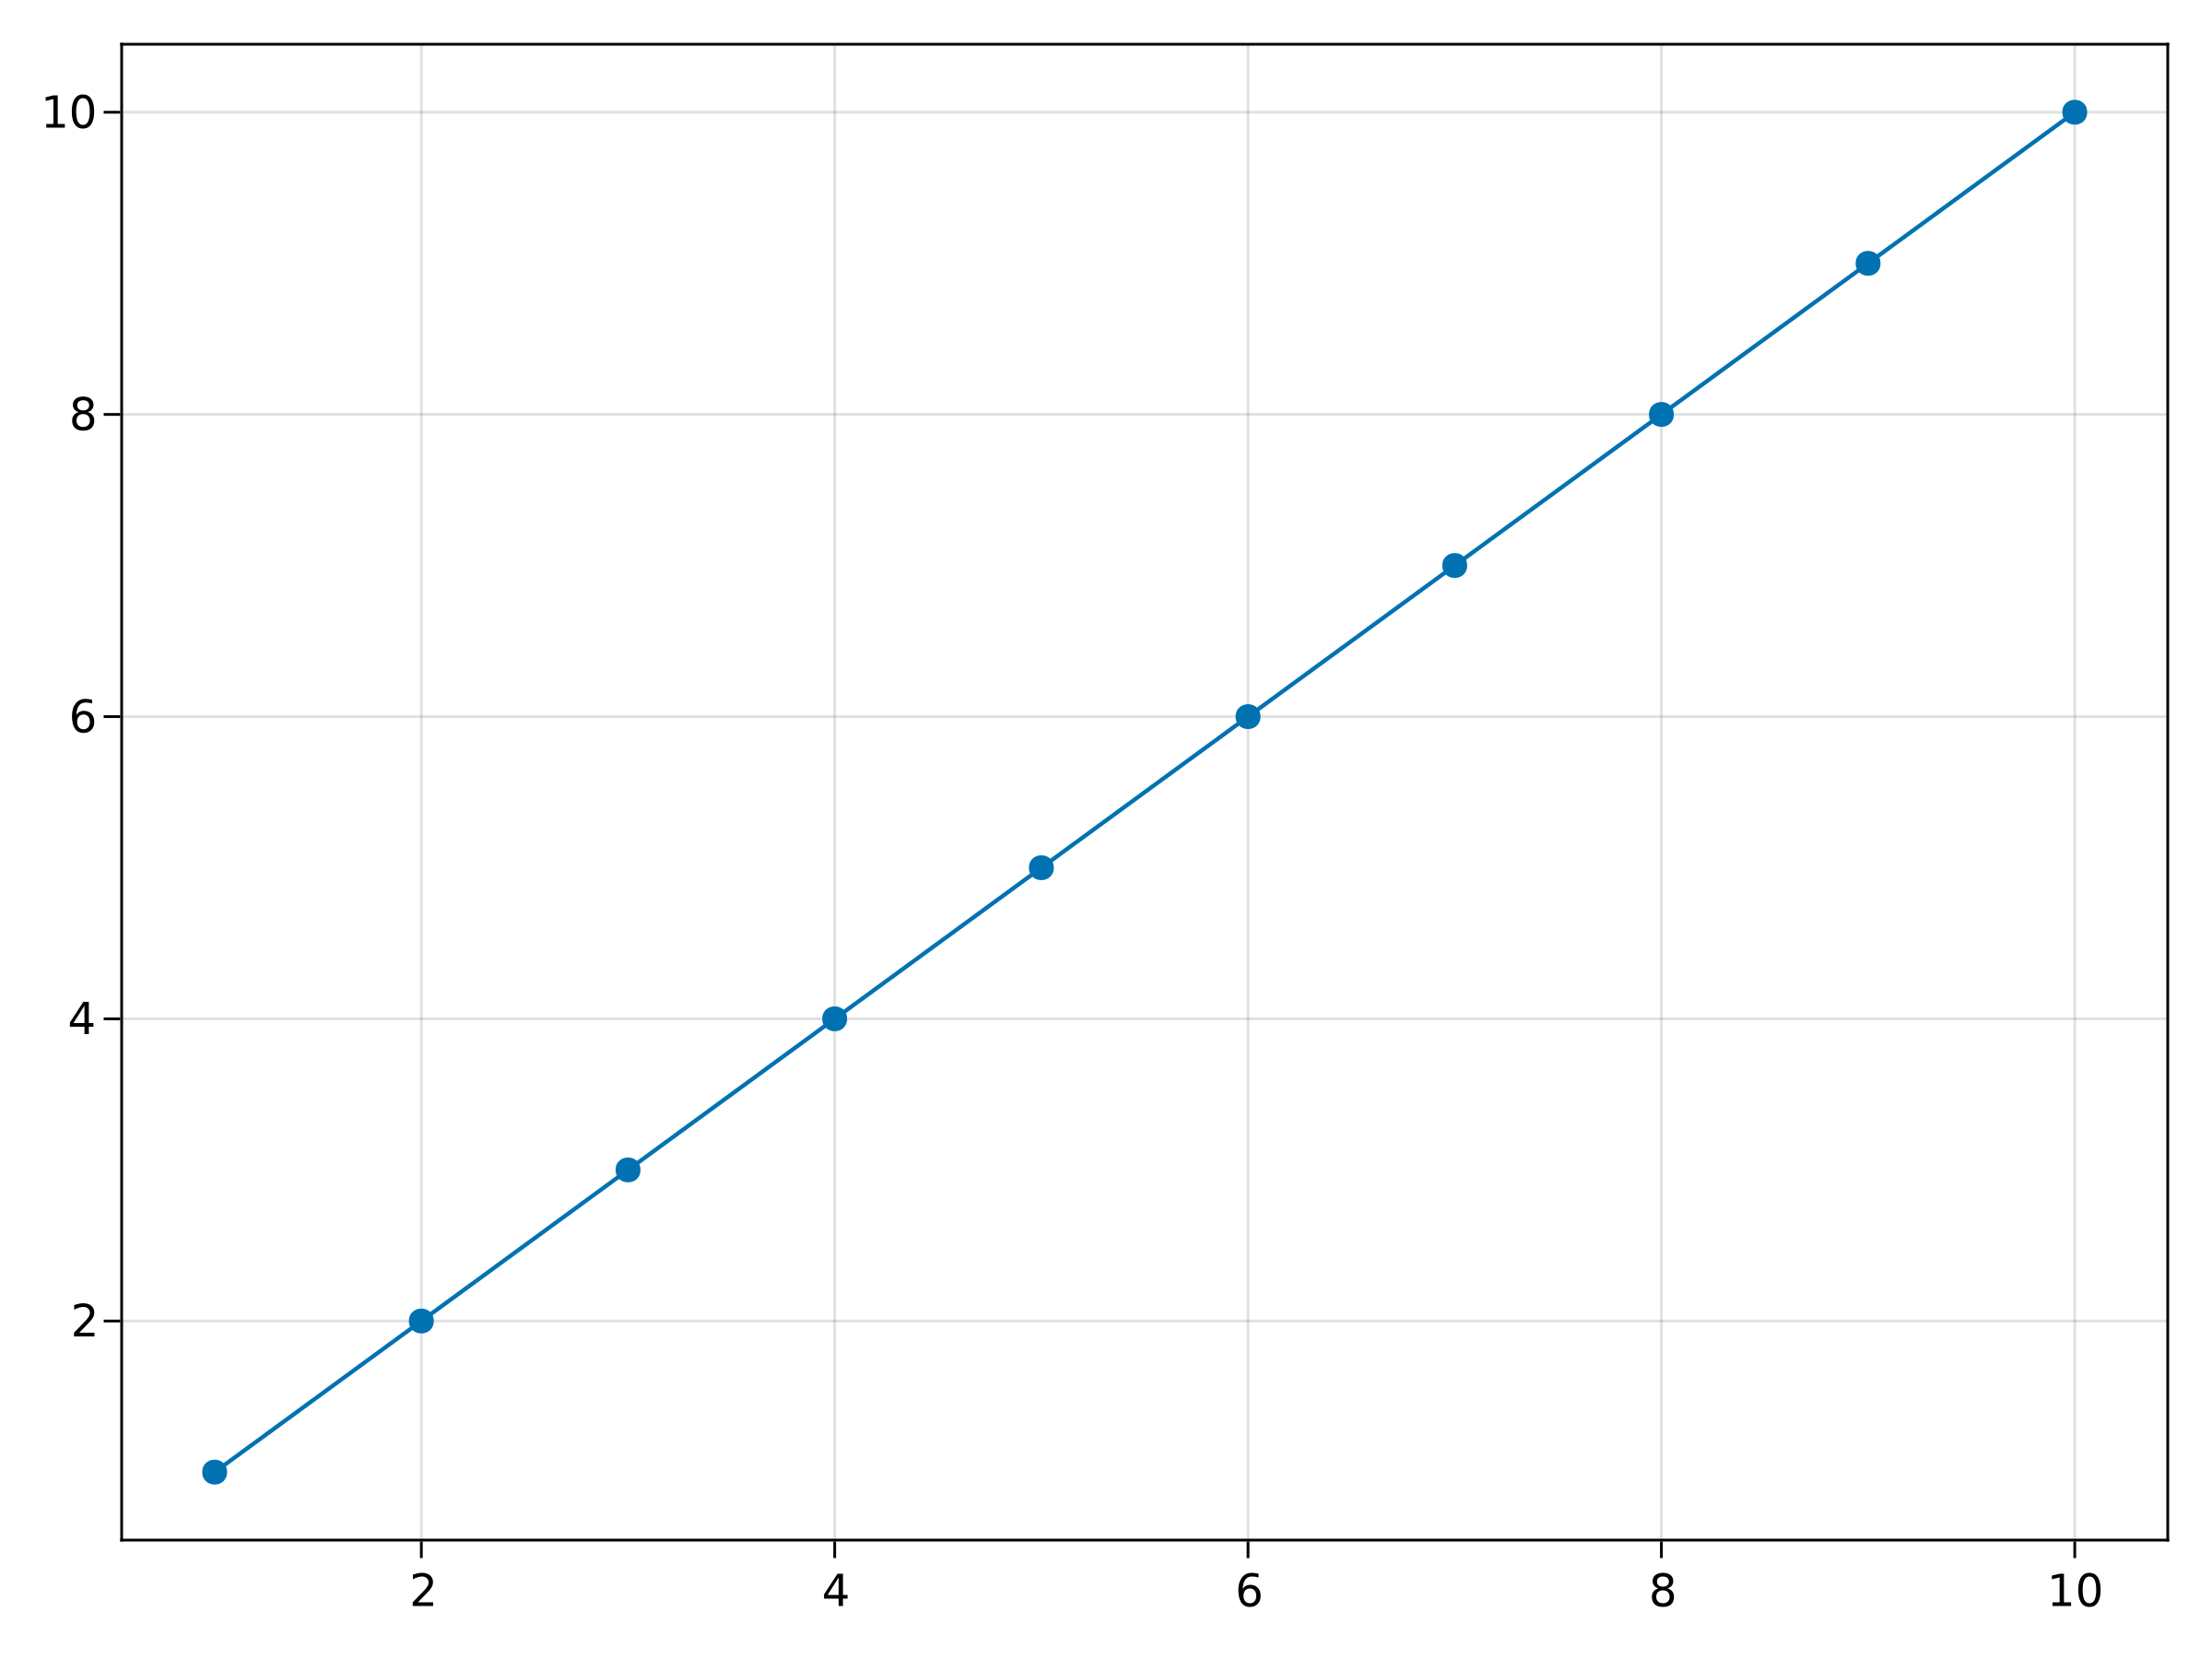
\includegraphics[width=0.6\textwidth,height=\textheight]{_build/im/firstplot.png}
\caption{First plot.}\label{fig:firstplot}
}
\end{figure}

注意前面的图采用默认输出样式,因此需要使用轴名称和轴标签进一步调整。

同时注意每一个像 \passthrough{\lstinline!scatterlines!}
这样的绘图函数都创建了一个 \passthrough{\lstinline!FigureAxisPlot!}
列表,其中包含 \passthrough{\lstinline!Figure!},
\passthrough{\lstinline!Axis!} 和 \passthrough{\lstinline!plot!} 对象。
这些函数也被称为 \passthrough{\lstinline!non-mutating!} 方法。
另一方面, \passthrough{\lstinline!mutating!} 方法(例如
\passthrough{\lstinline"scatterlines!"},注意多了
\passthrough{\lstinline"!"}) 仅返回一个 plot 对象,它可以被添加到给定的
\passthrough{\lstinline!axis!} 或
\passthrough{\lstinline!current\_figure()!} 中。

下一个问题是如何改变颜色或标记的类型? 这可以通过
\passthrough{\lstinline!attributes!} 实现, 将在下一节讨论。

\hypertarget{sec:datavisMakie_attributes}{%
\section{属性}\label{sec:datavisMakie_attributes}}

使用 \passthrough{\lstinline!attributes!} 可以创建自定义的图。
设置属性可以使用多个关键字参数。 每个 plot 对象的
\passthrough{\lstinline!attributes!} 列表可以通过以下方式查看:

\begin{lstlisting}[language=Julia]
fig, ax, pltobj = scatterlines(1:10)
pltobj.attributes
\end{lstlisting}

\begin{lstlisting}[language=Output]
Attributes with 15 entries:
  color => RGBA{Float32}(0.0,0.447059,0.698039,1.0)
  colormap => viridis
  colorrange => Automatic()
  cycle => [:color]
  inspectable => true
  linestyle => nothing
  linewidth => 1.5
  marker => Circle
  markercolor => Automatic()
  markercolormap => viridis
  markercolorrange => Automatic()
  markersize => 9
  model => Float32[1.0 0.0 0.0 0.0; 0.0 1.0 0.0 0.0; 0.0 0.0 1.0 0.0; 0.0 0.0 0.0 1.0]
  strokecolor => black
  strokewidth => 0
\end{lstlisting}

或者调用 \passthrough{\lstinline!pltobject.attributes.attributes!}
返回对象属性的\passthrough{\lstinline!Dict!} 。

对于任一给定的绘图函数,都能在 \passthrough{\lstinline!REPL!} 中以
\passthrough{\lstinline!?lines!} 或
\passthrough{\lstinline!help(lines)!}
的形式获取帮助。Julia将输出该函数的相应属性,并简要说明如何使用该函数。
关于 \passthrough{\lstinline!lines!} 的例子如下:

\begin{lstlisting}[language=Julia]
help(lines)
\end{lstlisting}

\begin{lstlisting}[language=Output]
  lines(positions)
  lines(x, y)
  lines(x, y, z)

  Creates a connected line plot for each element in (x, y, z), (x, y) or
  positions.

  │ Tip
  │
  │  You can separate segments by inserting NaNs.

  lines has the following function signatures:

    (Vector, Vector)
    (Vector, Vector, Vector)
    (Matrix)

  Available attributes for Lines are:

    color
    colormap
    colorrange
    cycle
    depth_shift
    diffuse
    inspectable
    linestyle
    linewidth
    nan_color
    overdraw
    shininess
    specular
    ssao
    transparency
    visible
\end{lstlisting}

不仅 plot 对象有属性,\passthrough{\lstinline!Axis!} 和
\passthrough{\lstinline!Figure!} 对象也有属性。 例如,Figure 的属性有
\passthrough{\lstinline!backgroundcolor!},\passthrough{\lstinline!resolution!},\passthrough{\lstinline!font!}
和 \passthrough{\lstinline!fontsize!} 以及
\passthrough{\lstinline!figure\_padding!}。 其中
\passthrough{\lstinline!figure\_padding!} 改变了图像周围的空白区域,如图
(图~\ref{fig:custom_plot}) 中的灰色区域所示。
它使用一个数字指定所有边的范围,或使用四个数的元组表示上下左右。

\passthrough{\lstinline!Axis!} 同样有一系列属性,典型的有
\passthrough{\lstinline!backgroundcolor!},
\passthrough{\lstinline!xgridcolor!} 和
\passthrough{\lstinline!title!}。 使用
\passthrough{\lstinline!help(Axis)!} 可查看所有属性。

在接下来这张图里,我们将设置一些属性:

\begin{lstlisting}[language=Julia]
lines(1:10, (1:10).^2; color=:black, linewidth=2, linestyle=:dash,
    figure=(; figure_padding=5, resolution=(600, 400), font="sans",
        backgroundcolor=:grey90, fontsize=16),
    axis=(; xlabel="x", ylabel="x²", title="title",
        xgridstyle=:dash, ygridstyle=:dash))
current_figure()
\end{lstlisting}

\begin{figure}
\hypertarget{fig:custom_plot}{%
\centering
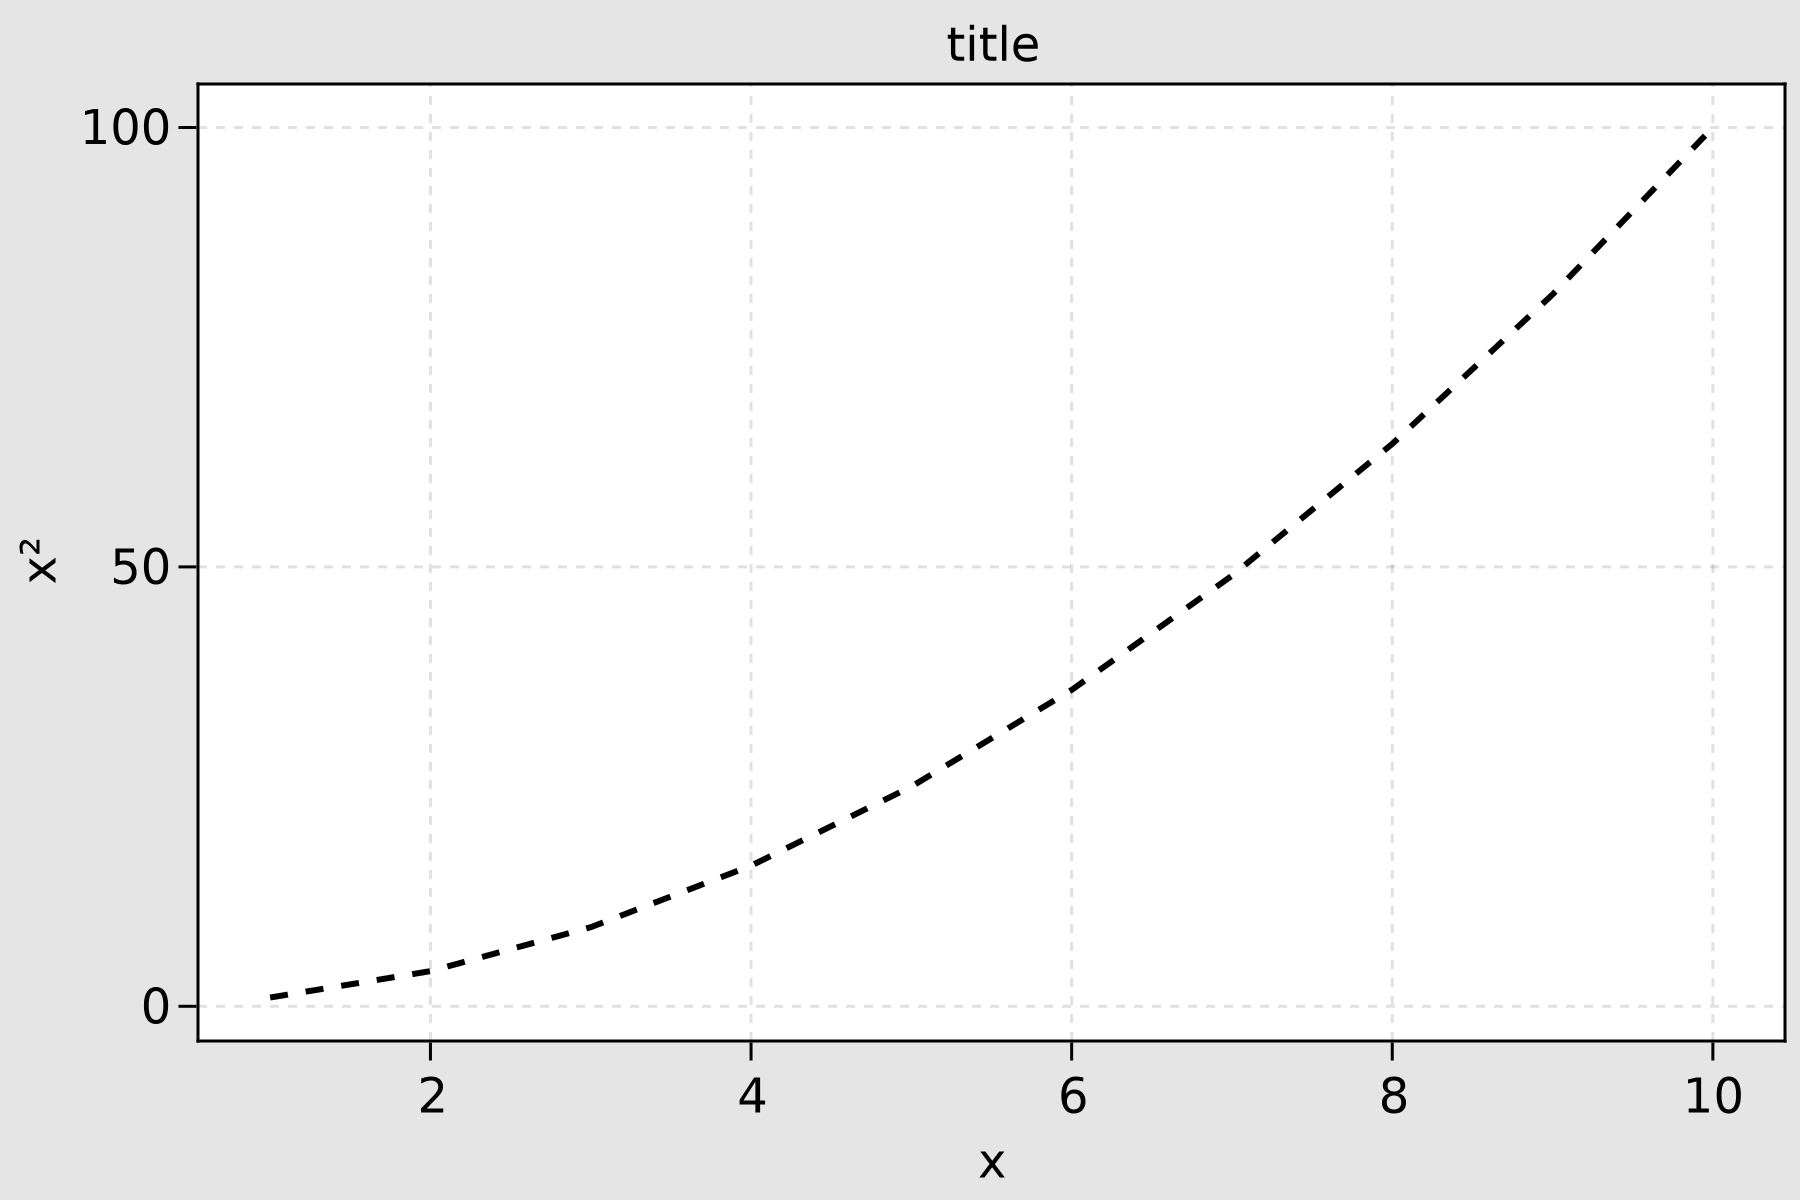
\includegraphics[width=0.6\textwidth,height=\textheight]{_build/im/custom_plot.png}
\caption{Custom plot.}\label{fig:custom_plot}
}
\end{figure}

此例已经包含了大多数用户经常会用到的属性。 或许在图上加一个
\passthrough{\lstinline!legend!} 会更好,这在有多条曲线时尤为有意义。
所以,向图上 \passthrough{\lstinline!append!} 另一个
\passthrough{\lstinline!plot object!} 并且通过调用
\passthrough{\lstinline!axislegend!} 添加对应的图例。 它将收集所有 plot
函数中的 \passthrough{\lstinline!labels!}, 并且图例默认位于图的右上角。
本例调用了 \passthrough{\lstinline!position=:ct!} 参数,其中
\passthrough{\lstinline!:ct!} 表示图例将位于
\passthrough{\lstinline!center!}和 \passthrough{\lstinline!top!}, 如图
图~\ref{fig:custom_plot_leg} 所示:

\begin{lstlisting}[language=Julia]
lines(1:10, (1:10).^2; label="x²", linewidth=2, linestyle=nothing,
    figure=(; figure_padding=5, resolution=(600, 400), font="sans",
        backgroundcolor=:grey90, fontsize=16),
    axis=(; xlabel="x", title="title", xgridstyle=:dash,
        ygridstyle=:dash))
scatterlines!(1:10, (10:-1:1).^2; label="Reverse(x)²")
axislegend("legend"; position=:ct)
current_figure()
\end{lstlisting}

\begin{figure}
\hypertarget{fig:custom_plot_leg}{%
\centering
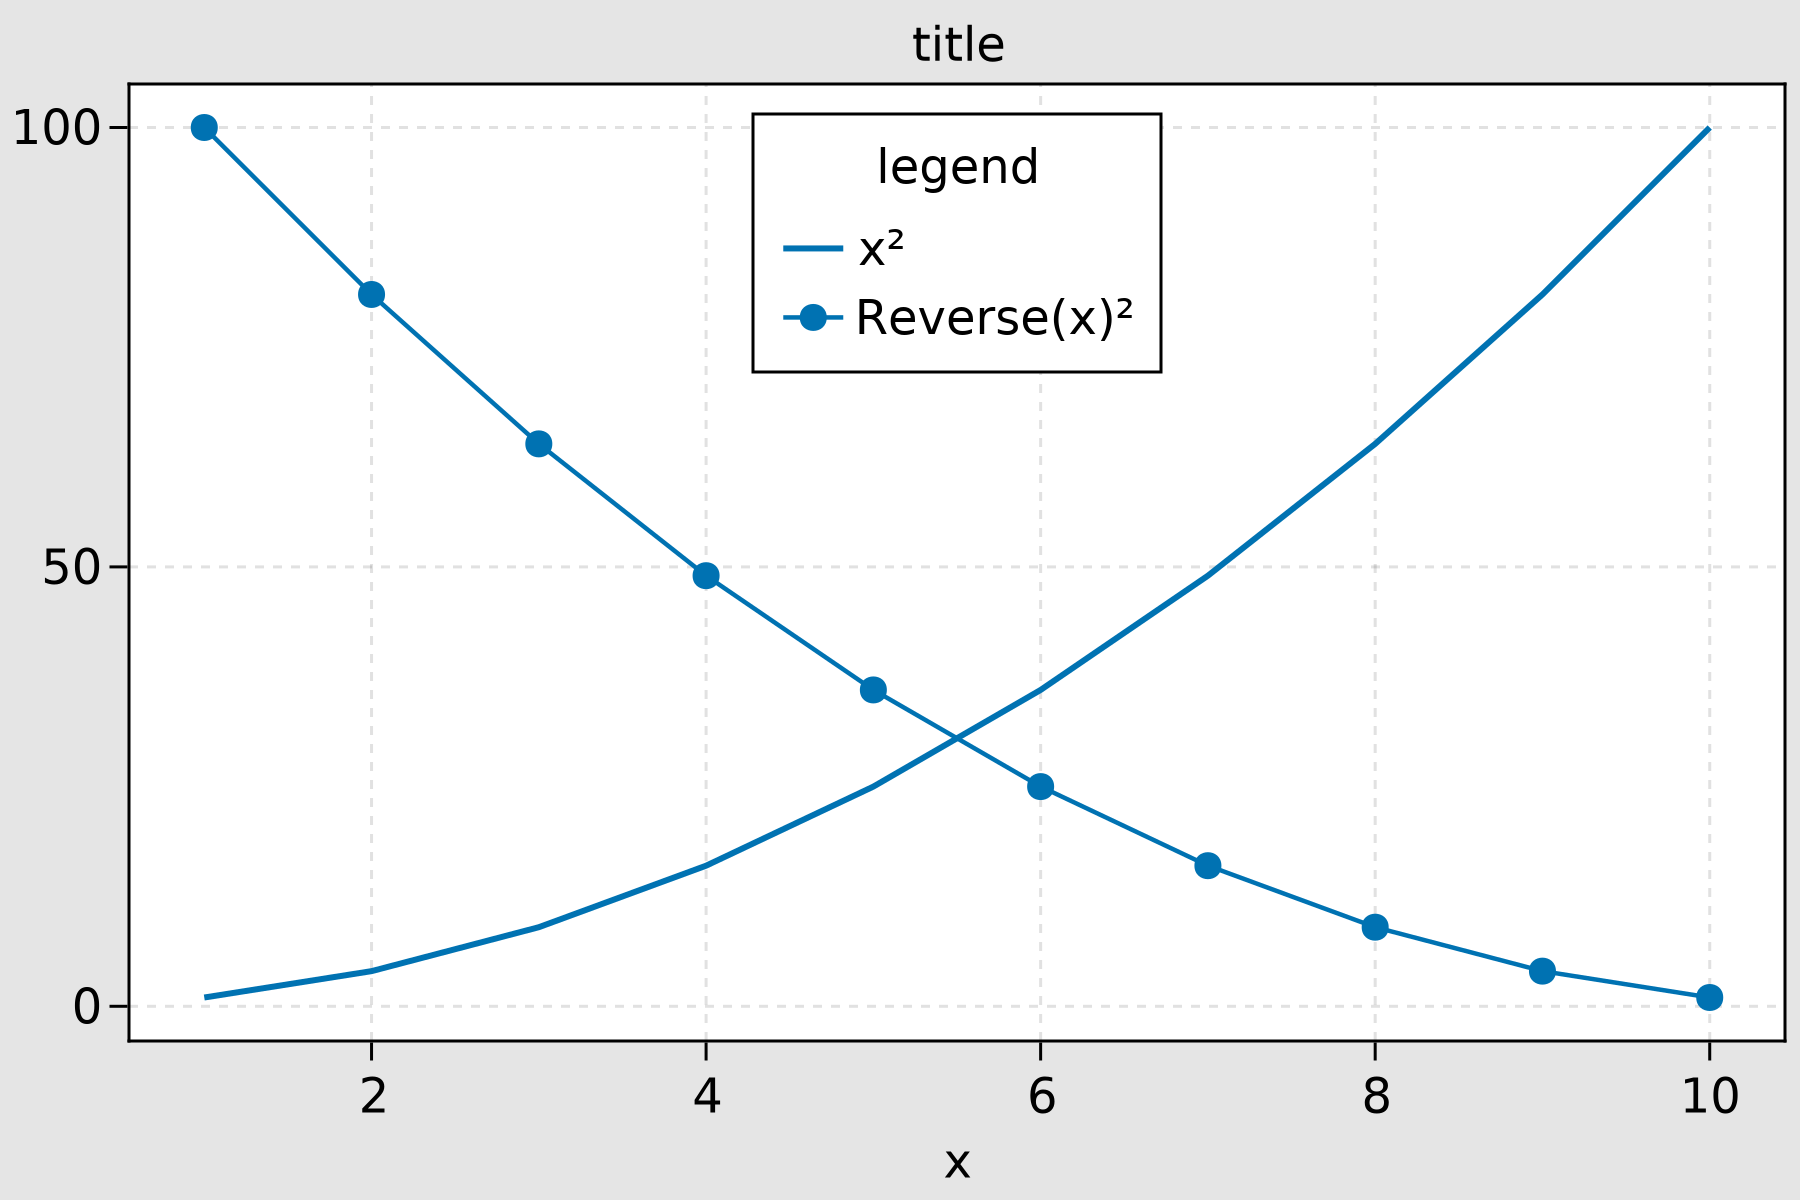
\includegraphics[width=0.6\textwidth,height=\textheight]{_build/im/custom_plot_leg.png}
\caption{Custom plot legend.}\label{fig:custom_plot_leg}
}
\end{figure}

通过组合 \passthrough{\lstinline!left(l), center(c), right(r)!} 和
\passthrough{\lstinline!bottom(b), center(c), top(t)!}
还可以再指定其他位置。 例如,使用\passthrough{\lstinline!:lt!}
指定为左上角。

然而,仅仅为两条曲线编写这么多代码是比较复杂的。
所以,如果要以相同的样式绘制一组曲线,那么最好指定一个主题。 使用
\passthrough{\lstinline"set\_theme!()"} 可实现该操作,如下所示。

使用
\passthrough{\lstinline"set\_theme!(kwargs)"}定义的新配置,重新绘制之前的图:

\begin{lstlisting}[language=Julia]
set_theme!(; resolution=(600, 400),
    backgroundcolor=(:orange, 0.5), fontsize=16, font="sans",
    Axis=(backgroundcolor=:grey90, xgridstyle=:dash, ygridstyle=:dash),
    Legend=(bgcolor=(:red, 0.2), framecolor=:dodgerblue))
lines(1:10, (1:10).^2; label="x²", linewidth=2, linestyle=nothing,
    axis=(; xlabel="x", title="title"))
scatterlines!(1:10, (10:-1:1).^2; label="Reverse(x)²")
axislegend("legend"; position=:ct)
current_figure()
set_theme!()
caption = "Set theme example."
\end{lstlisting}

\begin{figure}
\hypertarget{fig:setTheme}{%
\centering
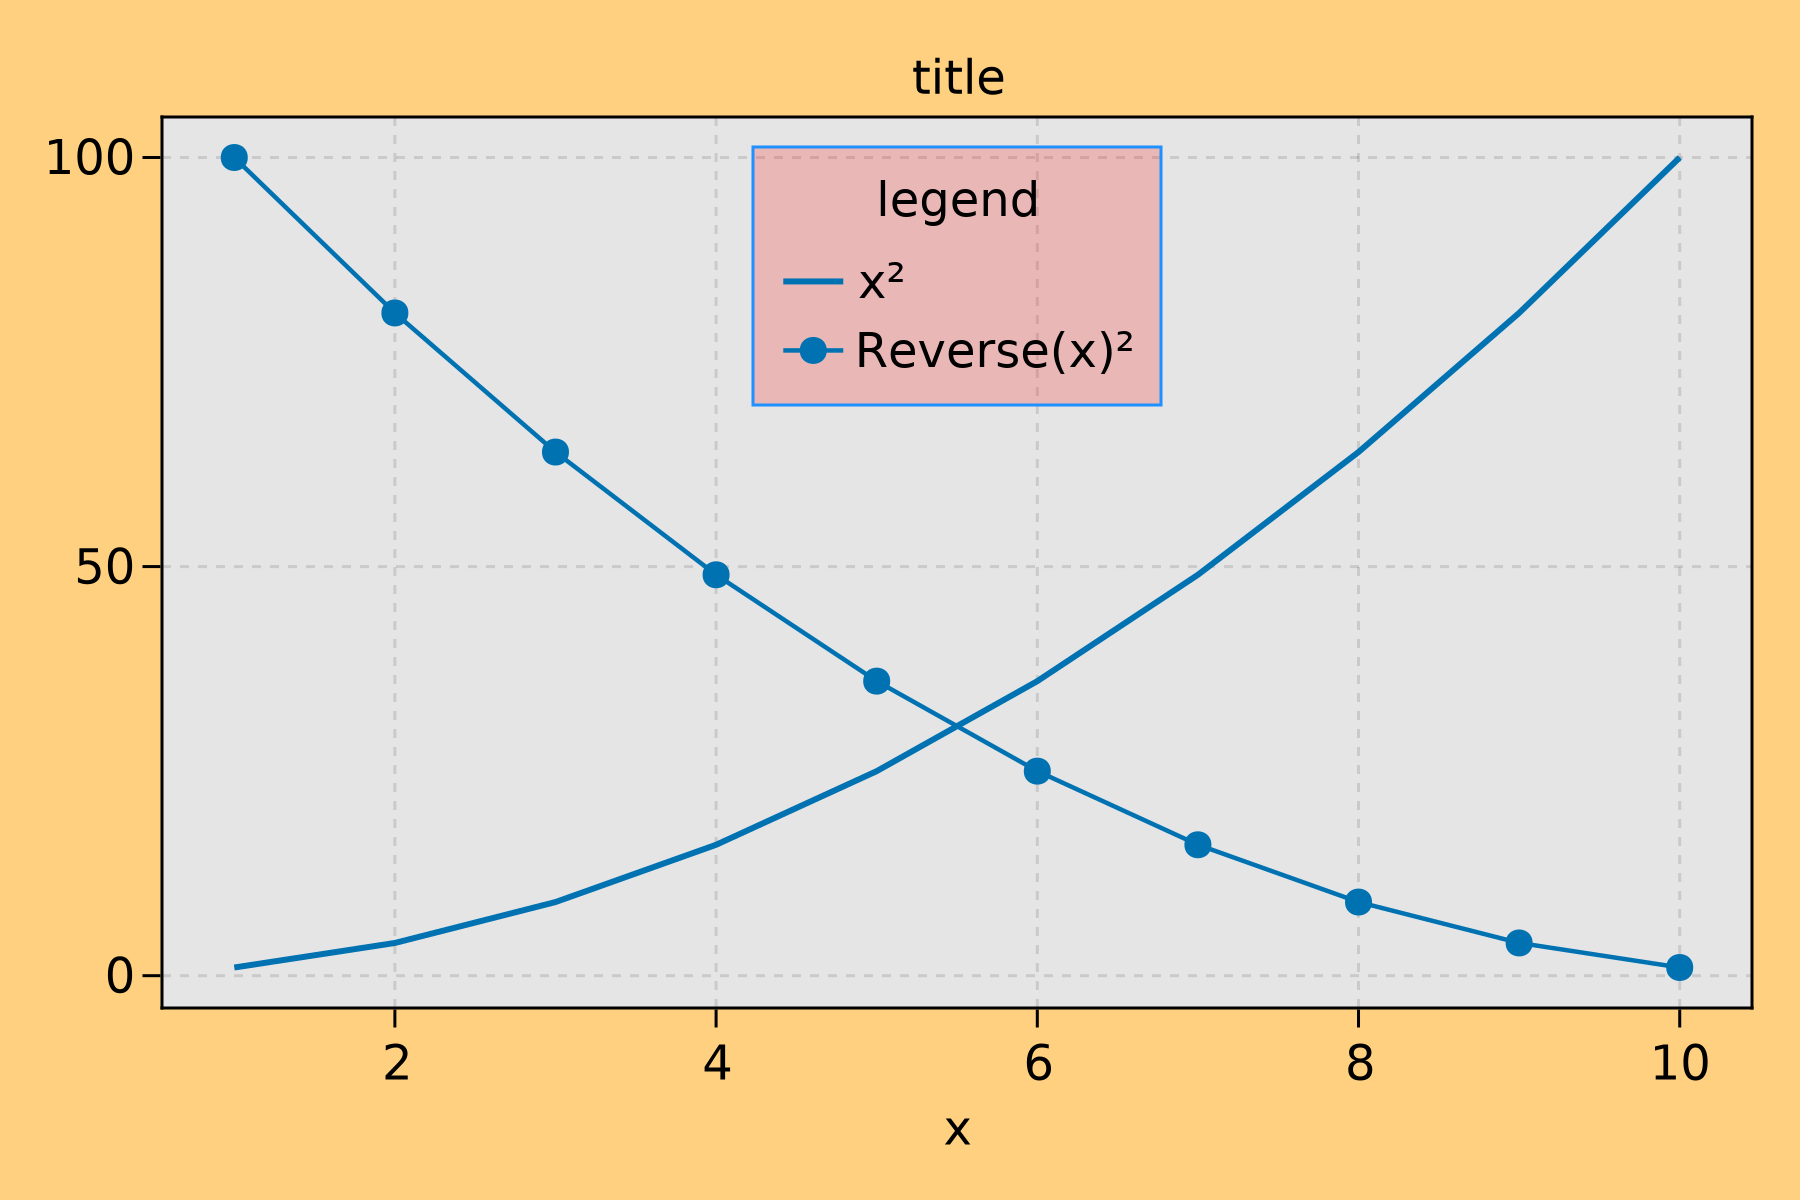
\includegraphics[width=0.6\textwidth,height=\textheight]{_build/im/setTheme.png}
\caption{Set theme example.}\label{fig:setTheme}
}
\end{figure}

倒数第二行的 \passthrough{\lstinline"set\_theme!()"} 会将主题重置到
Makie 的默认设置。 有关 \passthrough{\lstinline!themes!}
的更多内容请转到 Section~\ref{sec:themes}。

在进入下节前, 值得先看一个例子:将多个参数所组成的
\passthrough{\lstinline!array!} 传递给绘图函数来配置属性。 例如,使用
\passthrough{\lstinline!scatter!} 绘图函数绘制气泡图。

本例随机生成 100 行 3 列的 \passthrough{\lstinline!array!}
,这些数据满足正态分布。 其中第一列表示 \passthrough{\lstinline!x!}
轴上的位置,第二列表示 \passthrough{\lstinline!y!}
轴上的位置,第三列表示与每一点关联的属性值。 例如可以用来指定不同的
\passthrough{\lstinline!color!}
或者不同的标记大小。气泡图就可以实现相同的操作。

\begin{lstlisting}[language=Julia]
using Random: seed!
seed!(28)
xyvals = randn(100, 3)
xyvals[1:5, :]
\end{lstlisting}

\begin{lstlisting}[language=Output]
5×3 Matrix{Float64}:
  0.550992   1.27614    -0.659886
 -1.06587   -0.0287242   0.175126
 -0.721591  -1.84423     0.121052
  0.801169   0.862781   -0.221599
 -0.340826   0.0589894  -1.76359
\end{lstlisting}

对应的图 图~\ref{fig:bubble} 如下所示:

\begin{lstlisting}[language=Julia]
fig, ax, pltobj = scatter(xyvals[:, 1], xyvals[:, 2]; color=xyvals[:, 3],
    label="Bubbles", colormap=:plasma, markersize=15 * abs.(xyvals[:, 3]),
    figure=(; resolution=(600, 400)), axis=(; aspect=DataAspect()))
limits!(-3, 3, -3, 3)
Legend(fig[1, 2], ax, valign=:top)
Colorbar(fig[1, 2], pltobj, height=Relative(3 / 4))
fig
caption = "Bubble plot."
\end{lstlisting}

\begin{figure}
\hypertarget{fig:bubble}{%
\centering
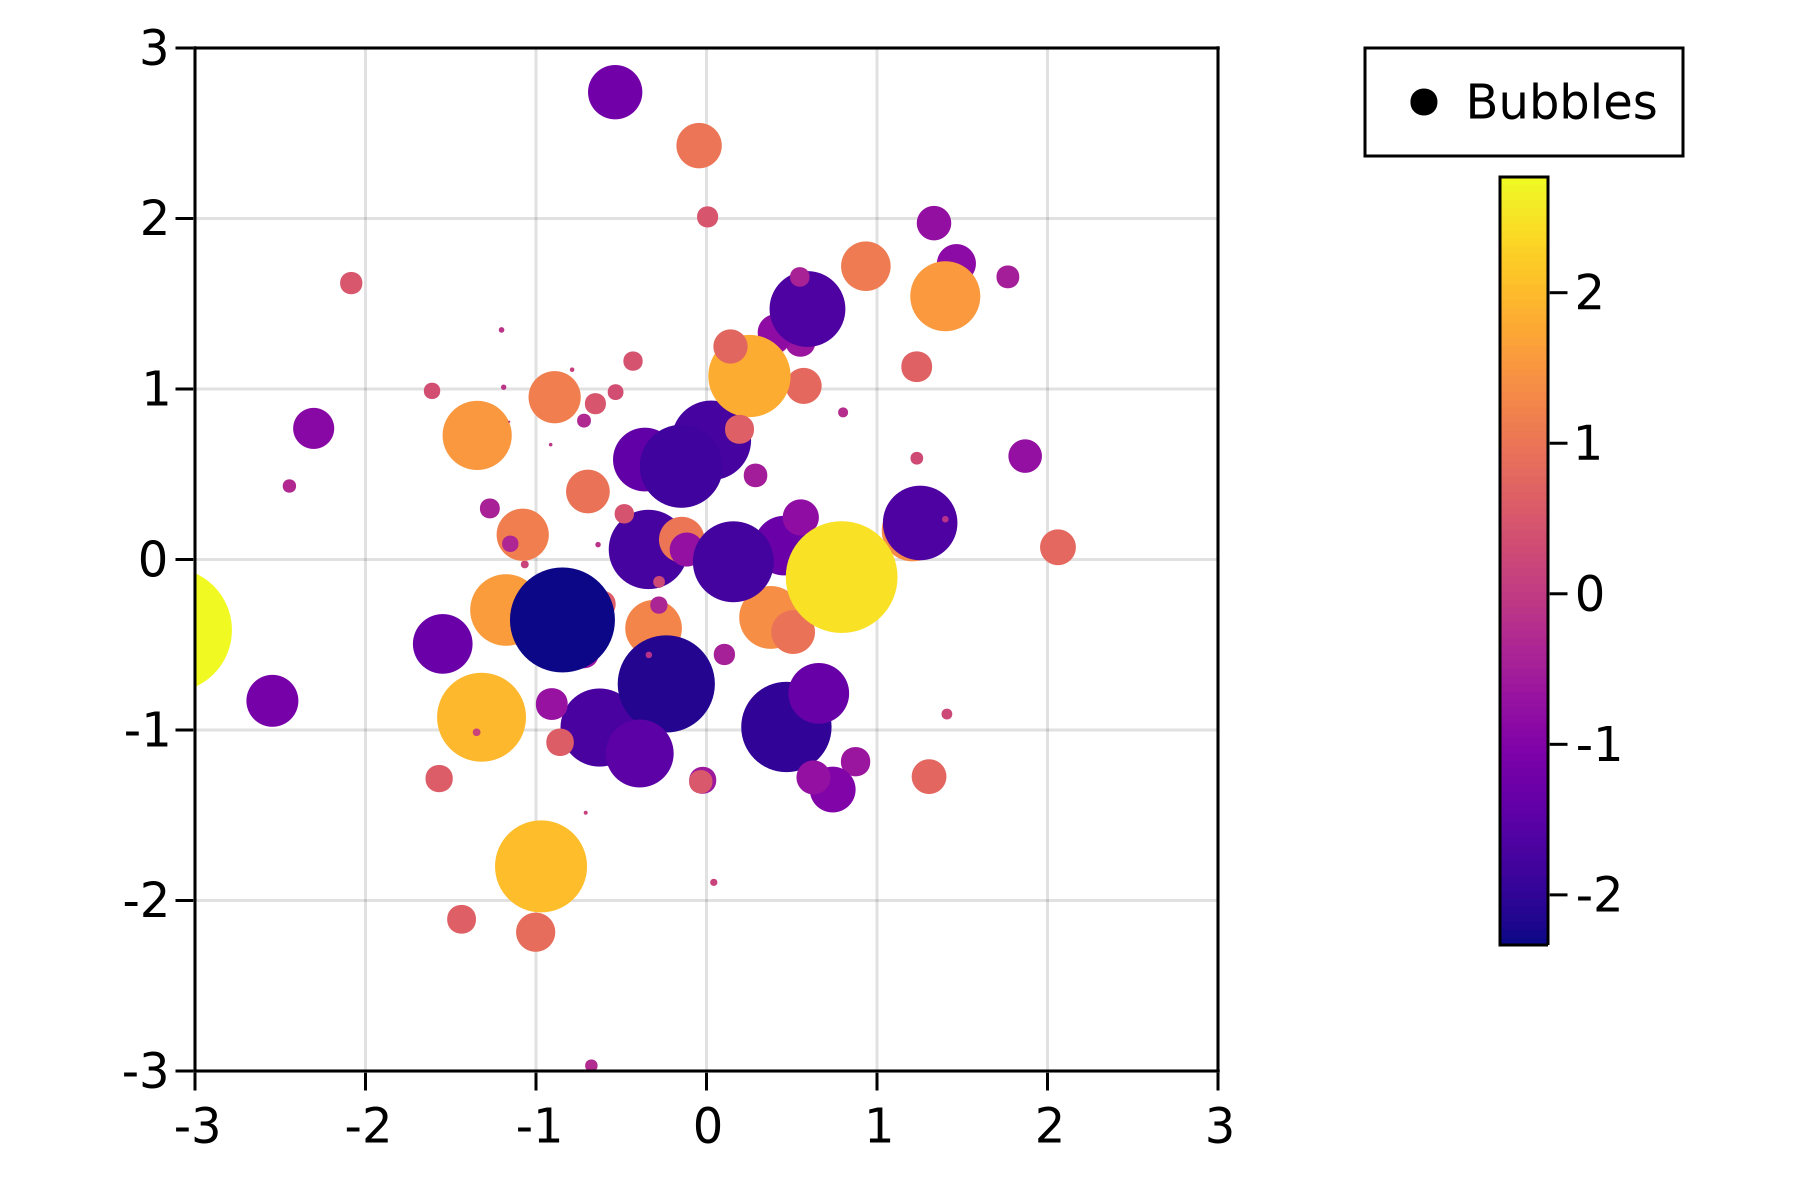
\includegraphics[width=0.6\textwidth,height=\textheight]{_build/im/bubble.png}
\caption{Bubble plot.}\label{fig:bubble}
}
\end{figure}

为了在图上添加 \passthrough{\lstinline!Legend!} 和
\passthrough{\lstinline!Colorbar!},需将
\passthrough{\lstinline!FigureAxisPlot!} 元组分解为
\passthrough{\lstinline!fig, ax, pltobj!}。 我们将在
Section~\ref{sec:makie_layouts} 讨论有关布局选项的更多细节。

通过一些基本且有趣的例子,我们展示了如何使用\passthrough{\lstinline!Makie.jl!},现在你可能想知道:还能做什么?
\passthrough{\lstinline!Makie.jl!} 都还有哪些绘图函数?
为了回答此问题,我们制作了一个 \emph{cheat sheet} 如
图~\ref{fig:cheat_sheet_cairomakie} 所示。 使用
\passthrough{\lstinline!CairoMakie.jl!} 后端可以轻松绘制这些图。

\begin{figure}
\hypertarget{fig:cheat_sheet_cairomakie}{%
\centering
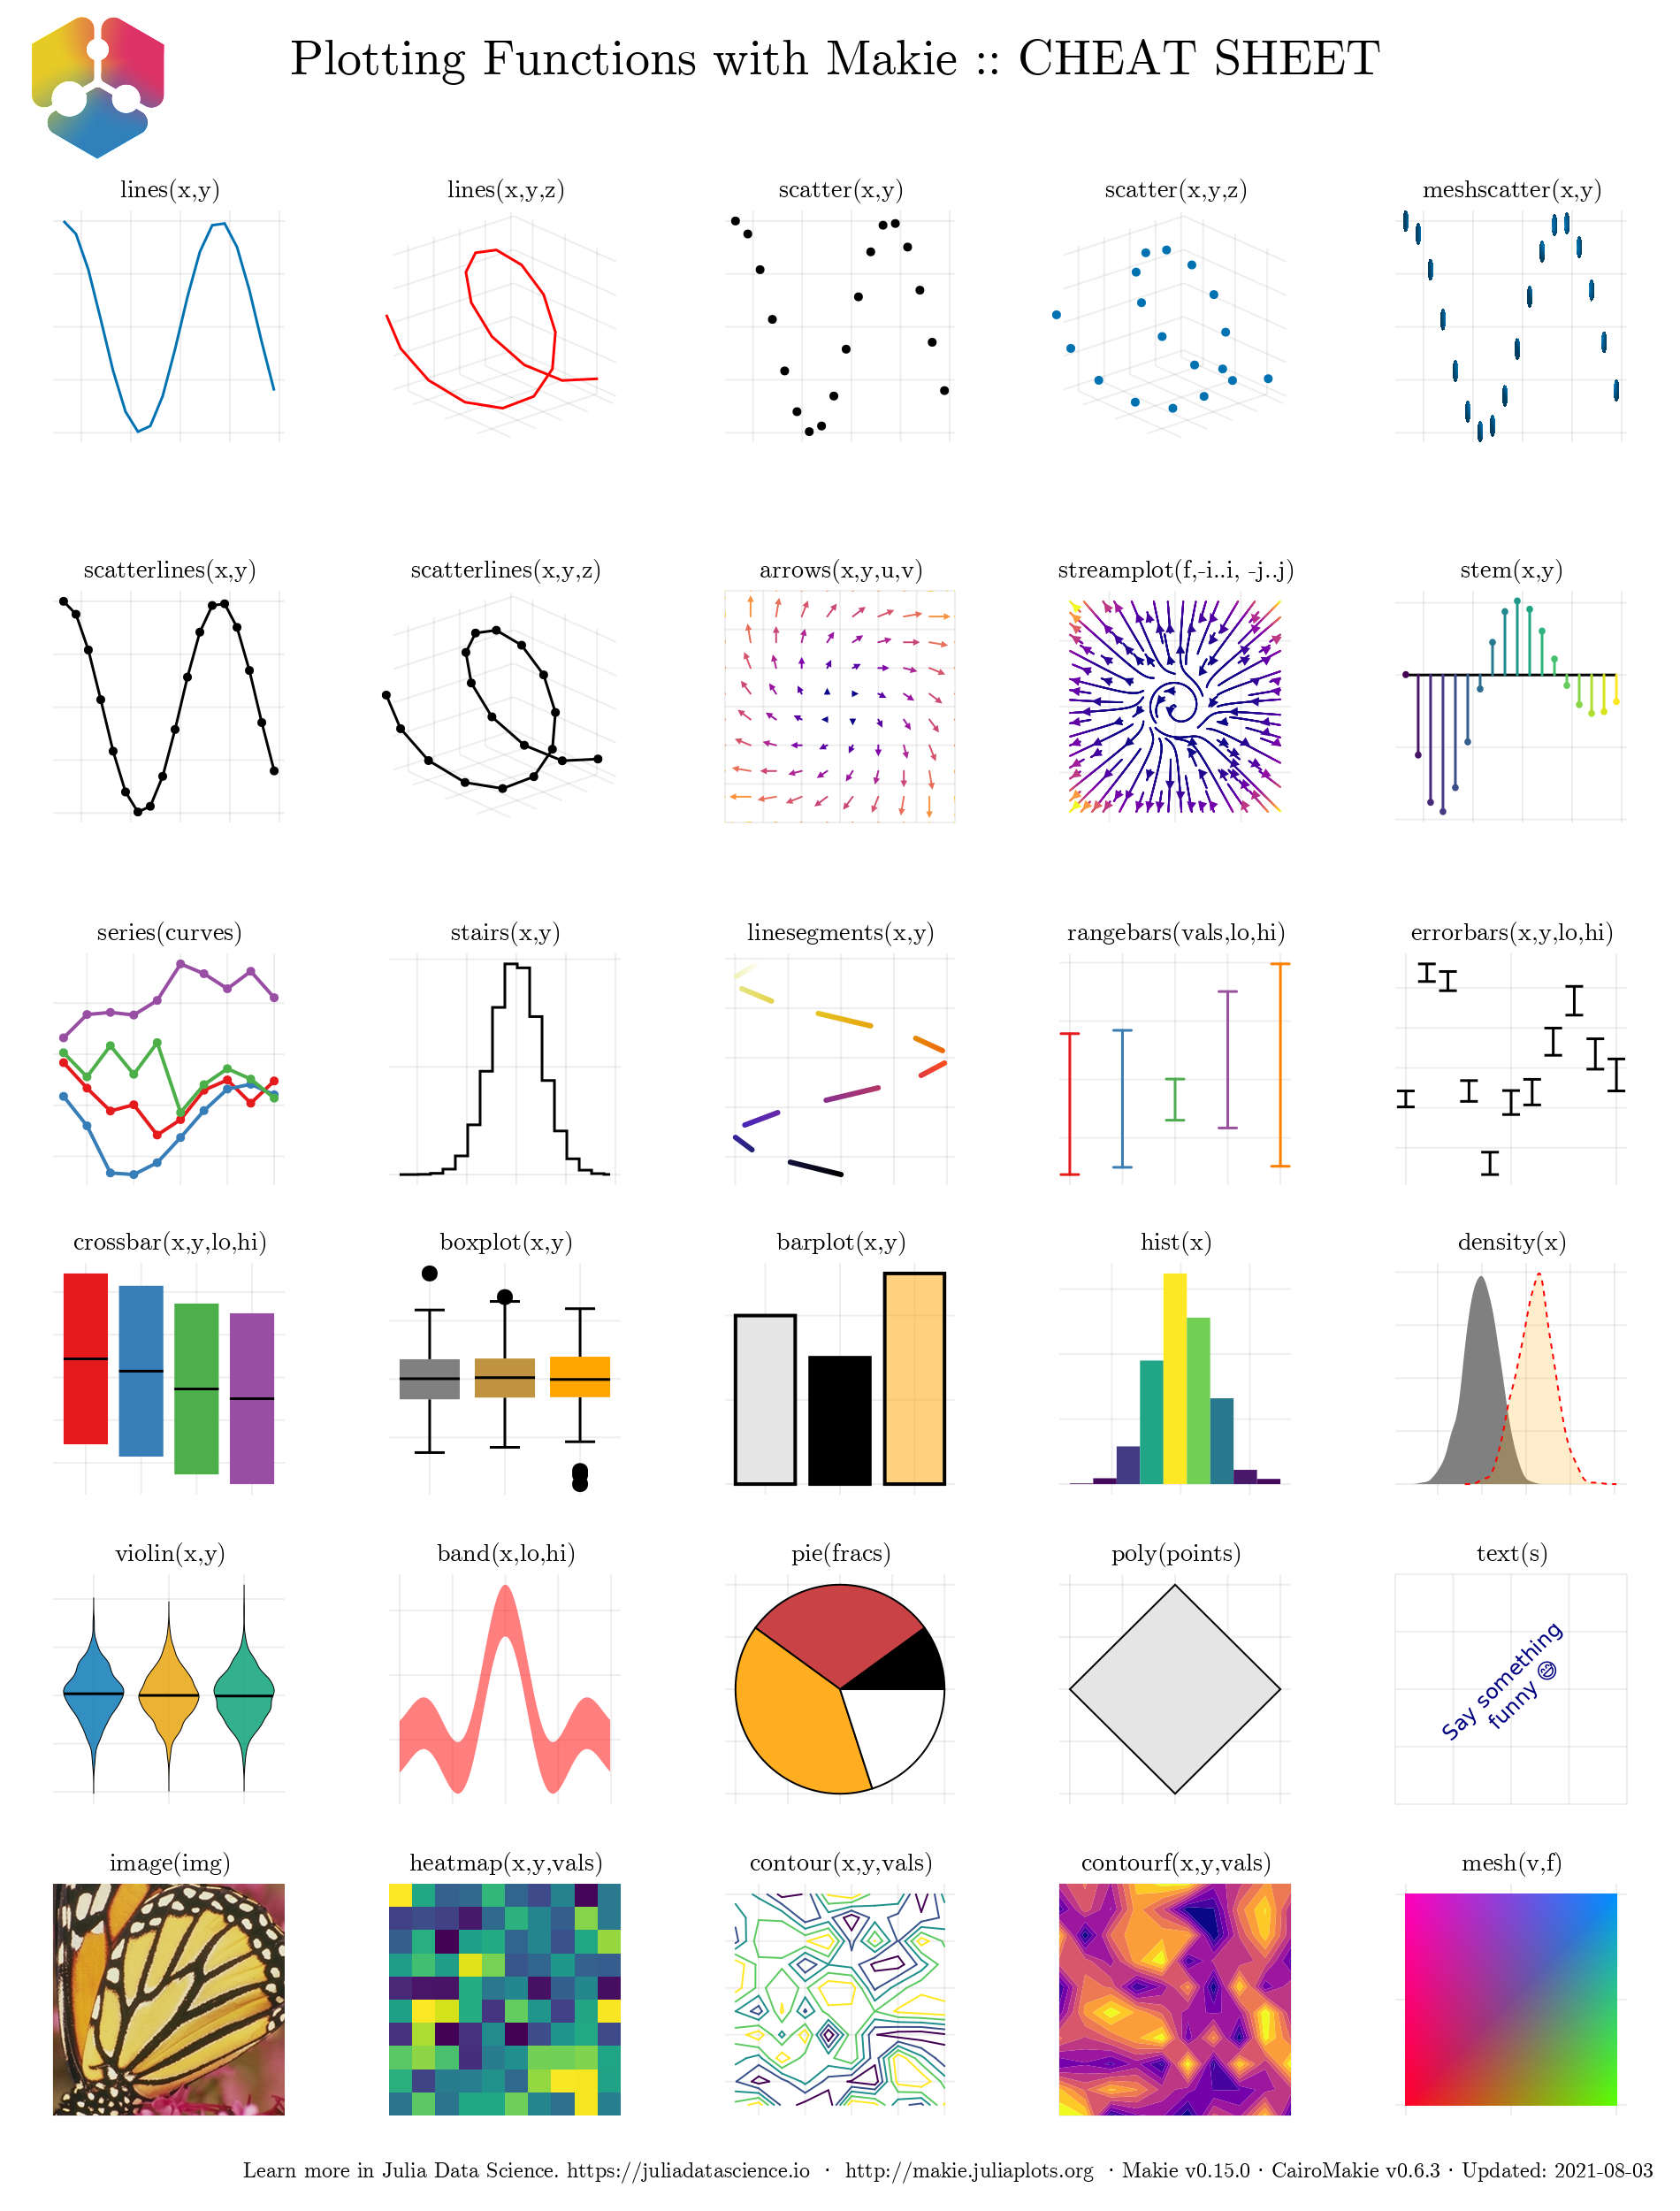
\includegraphics{images/makiePlottingFunctionsHide.png}
\caption{Plotting functions: Cheat Sheet. Output given by
Cairomakie.}\label{fig:cheat_sheet_cairomakie}
}
\end{figure}

图~\ref{fig:cheat_sheet_glmakie} 展示了
\passthrough{\lstinline!GLMakie.jl!} 的\_cheat sheet\_
,这些函数支持绘制大多数 3D 图。 这些将在后面的
\passthrough{\lstinline!GLMakie.jl!} 节进一步讨论。

\begin{figure}
\hypertarget{fig:cheat_sheet_glmakie}{%
\centering
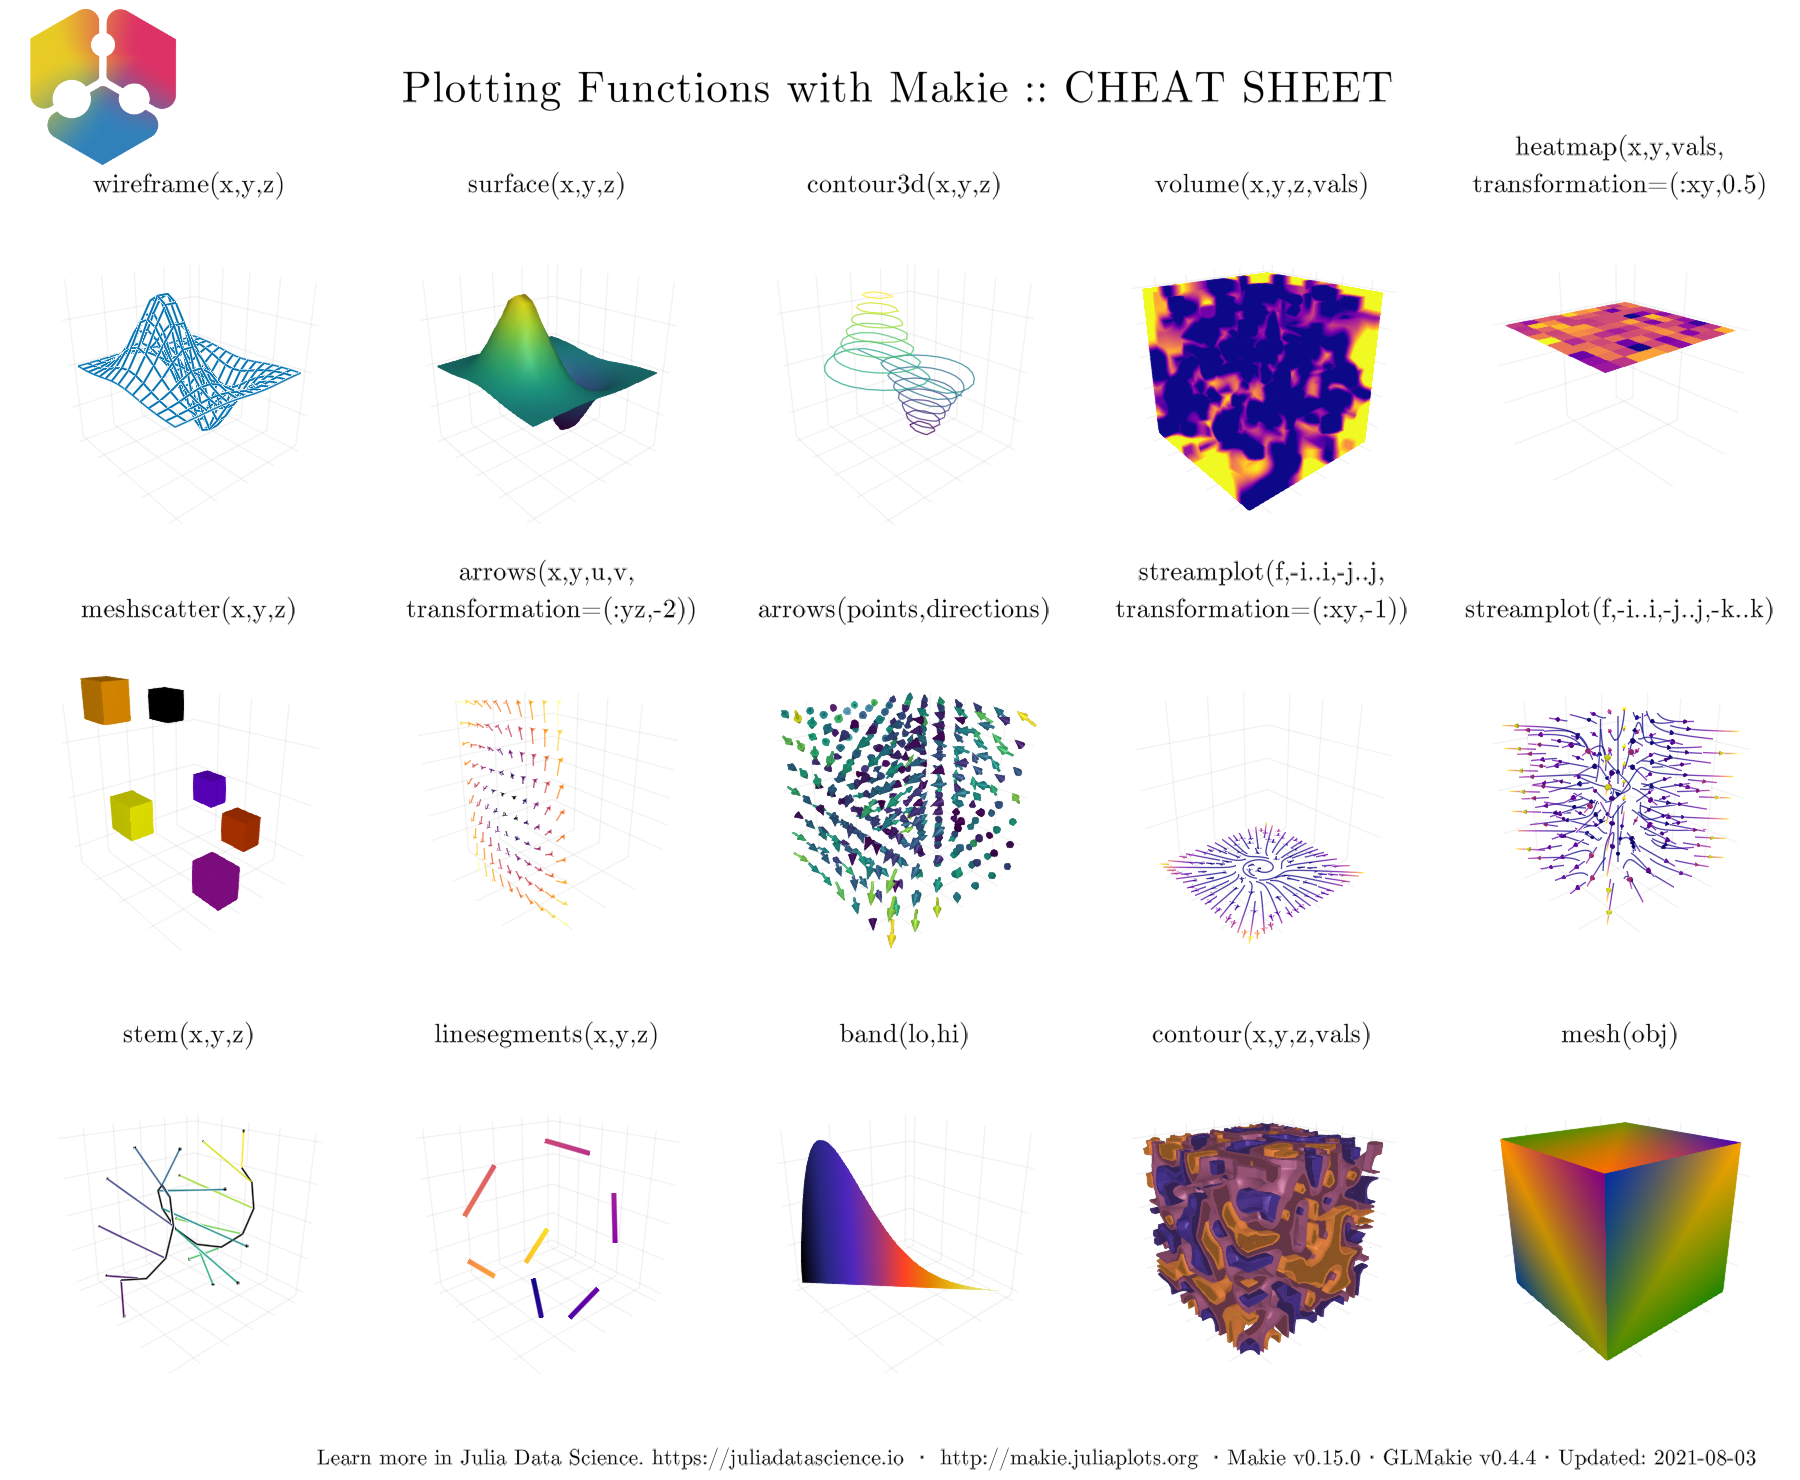
\includegraphics{images/GLMakiePlottingFunctionsHide.png}
\caption{Plotting functions: Cheat Sheet. Output given by
GLMakie.}\label{fig:cheat_sheet_glmakie}
}
\end{figure}

现在,我们已经大致了解到能做什么。接下来应该掉过头来继续研究基础知识。
是时候学习如何改变图的整体外观了。

\hypertarget{sec:themes}{%
\section{主题}\label{sec:themes}}

有多种方式可以改变图的整体外观。你可以使用
\href{http://makie.juliaplots.org/stable/documentation/theming/predefined_themes/index.html}{预定义主题}
或自定义的主题。例如,通过
\passthrough{\lstinline!with\_theme(your\_plot\_function, theme\_dark())!}
使用预定义的暗色主题。另外,也可以使用
\passthrough{\lstinline!Theme(kwargs)!} 构建你自己的主题或使用
\passthrough{\lstinline"update\_theme!(kwargs)"} 更新当前激活的主题。

还可以使用 \passthrough{\lstinline"set\_theme!(theme; kwargs...)"}
将当前主题改为 \passthrough{\lstinline!theme!}, 并且通过
\passthrough{\lstinline!kwargs!} 覆盖或增加一些属性。使用不带参数的
\passthrough{\lstinline"set\_theme!()"}
即可恢复到之前主题的设置。在下面的例子中,我们准备了具有不同样式的测试绘图函数,以便于观察每个主题的大多数属性。

\begin{lstlisting}[language=Julia]
using Random: seed!
seed!(123)
y = cumsum(randn(6, 6), dims=2)
\end{lstlisting}

\begin{lstlisting}[language=Output]
6×6 Matrix{Float64}:
  0.808288   0.386519   0.355371   0.0365011  -0.0911358   1.8115
 -1.12207   -2.47766   -2.16183   -2.49928    -2.02981    -1.37017
 -1.10464   -1.03518   -3.19756   -1.18944    -2.71633    -3.80455
 -0.416993  -0.534315  -1.42439   -0.659362   -0.0592298   0.644529
  0.287588   1.50687    2.36111    2.54137     0.48751     0.630836
  0.229819   0.522733   0.864515   2.89343     2.06537     2.21375
\end{lstlisting}

本例随机生成了一个大小为 \passthrough{\lstinline!(20,20)!}
的矩阵,以便于绘制一张热力图(heatmap)。 同时本例也指定了 \(x\) 和
\(y\) 的范围。

\begin{lstlisting}[language=Julia]
using Random: seed!
seed!(13)
xv = yv = LinRange(-3, 0.5, 20)
matrix = randn(20, 20)
matrix[1:6, 1:6] # first 6 rows and columns
\end{lstlisting}

\begin{lstlisting}[language=Output]
6×6 Matrix{Float64}:
 -0.271257   0.894952   0.728865  -0.293849   -0.449277   -0.0948871
 -0.193033  -0.421286  -0.455905  -0.0576092  -0.756621   -1.47419
 -0.123177   0.762254   0.773921  -0.38526    -0.0659695  -0.599284
 -1.47327    0.770122   1.20725    0.257913    0.111979    0.875439
 -1.82913   -0.603888   0.164083  -0.118504    1.46723     0.0948876
  1.09769    0.178207   0.110243  -0.543203    0.592245    0.328993
\end{lstlisting}

因此,新绘图函数如下所示:

\begin{lstlisting}[language=Julia]
function demo_themes(y, xv, yv, matrix)
    fig, _ = series(y; labels=["$i" for i = 1:6], markersize=10,
        color=:Set1, figure=(; resolution=(600, 300)),
        axis=(; xlabel="time (s)", ylabel="Amplitude",
            title="Measurements"))
    hmap = heatmap!(xv, yv, matrix; colormap=:plasma)
    limits!(-3.1, 8.5, -6, 5.1)
    axislegend("legend"; merge=true)
    Colorbar(fig[1, 2], hmap)
    fig
end
\end{lstlisting}

注意,\passthrough{\lstinline!series!}
函数的作用是同时绘制多条附带标签的直线图和散点图。另外还绘制了附带
colorbar 的 heatmap。如图所示,有两种暗色主题,一种是
\passthrough{\lstinline!theme\_dark()!} ,另一种是
\passthrough{\lstinline!theme\_black()!}。

\begin{lstlisting}[language=Julia]
with_theme(theme_dark()) do
    demo_themes(y, xv, yv, matrix)
end
with_theme(theme_black()) do
    demo_themes(y, xv, yv, matrix)
end
\end{lstlisting}

\begin{figure}
\hypertarget{fig:theme_dark}{%
\centering
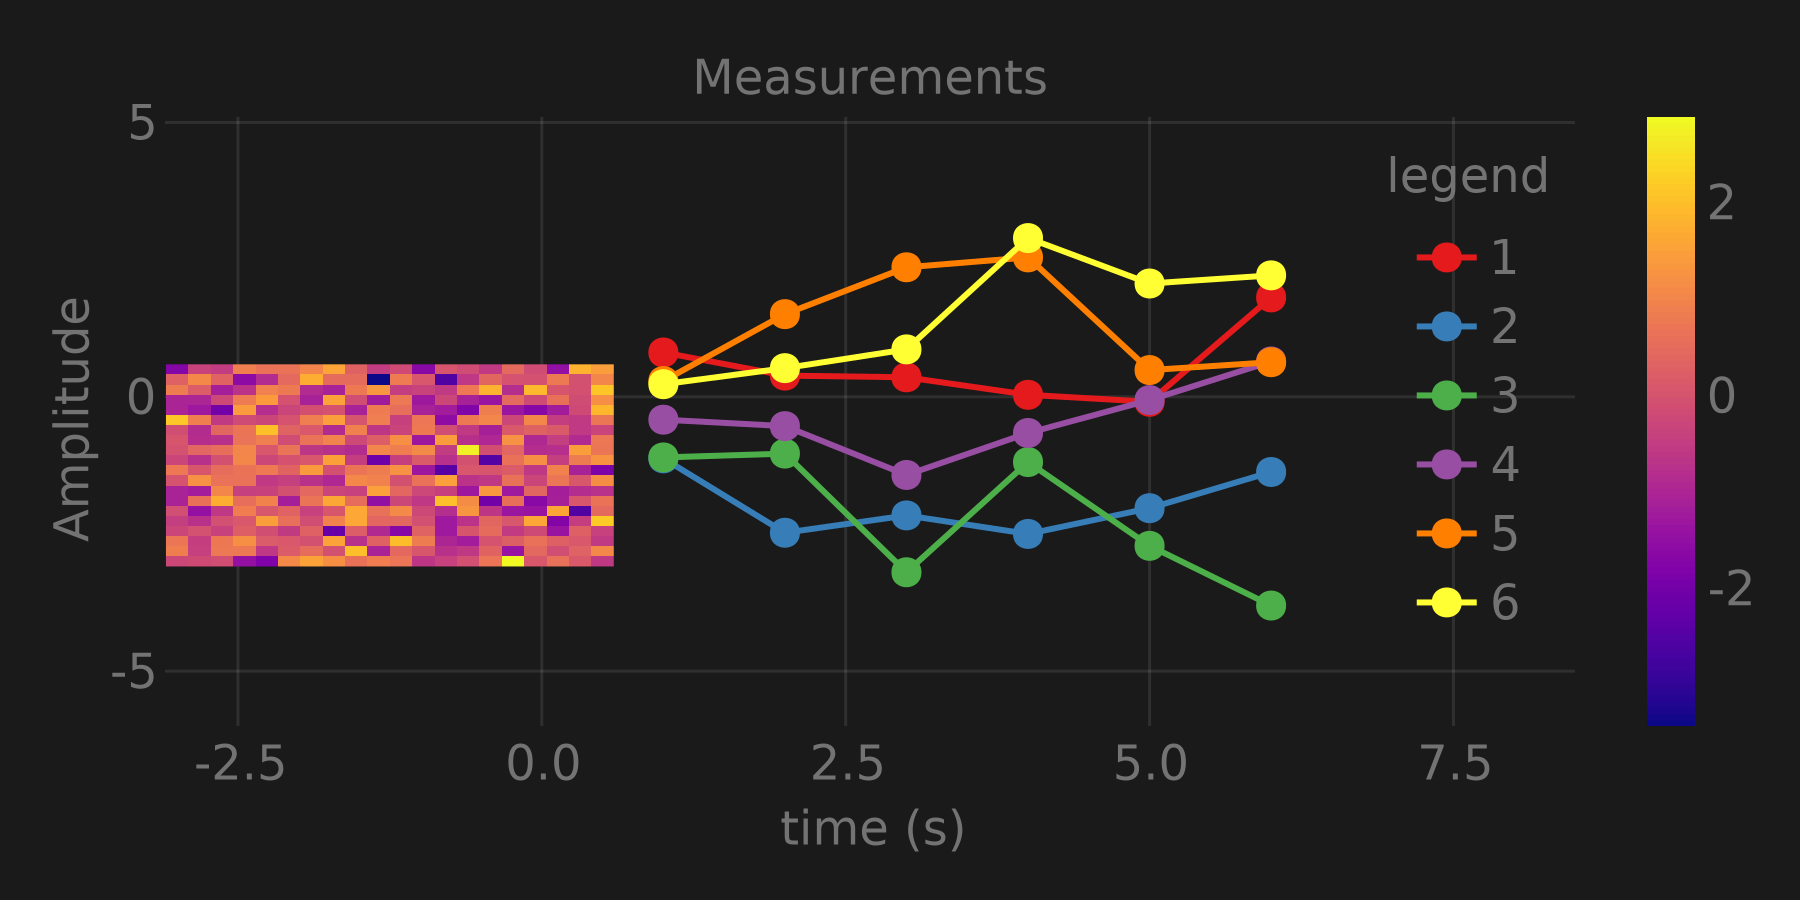
\includegraphics[width=0.6\textwidth,height=\textheight]{_build/im/theme_dark.png}
\caption{Theme dark.}\label{fig:theme_dark}
}
\end{figure}

\begin{figure}
\hypertarget{fig:theme_black}{%
\centering
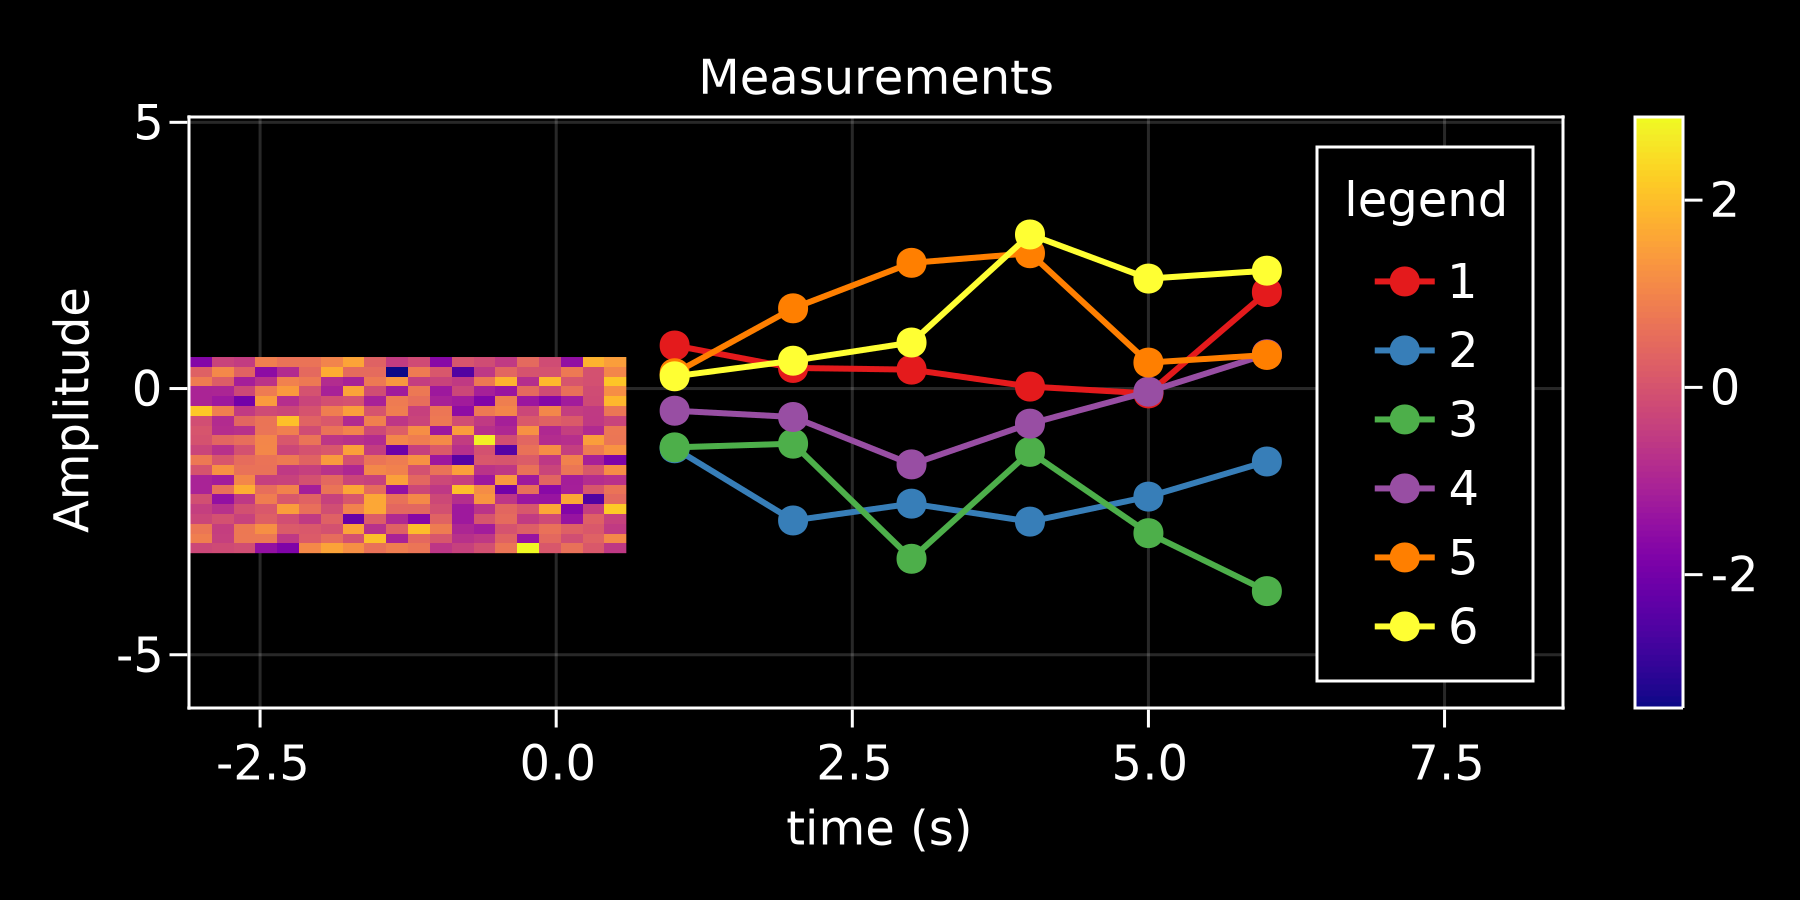
\includegraphics[width=0.6\textwidth,height=\textheight]{_build/im/theme_black.png}
\caption{Theme black.}\label{fig:theme_black}
}
\end{figure}

另外有三种白色主题,\passthrough{\lstinline!theme\_ggplot2()!},\passthrough{\lstinline!theme\_minimal()!}
和
\passthrough{\lstinline!theme\_light()!}。这些主题对于更标准的出版图很有用。

\begin{lstlisting}[language=Julia]
with_theme(theme_ggplot2()) do
    demo_themes(y, xv, yv, matrix)
end
with_theme(theme_minimal()) do
    demo_themes(y, xv, yv, matrix)
end
with_theme(theme_light()) do
    demo_themes(y, xv, yv, matrix)
end
\end{lstlisting}

\begin{figure}
\hypertarget{fig:theme_ggplot2}{%
\centering
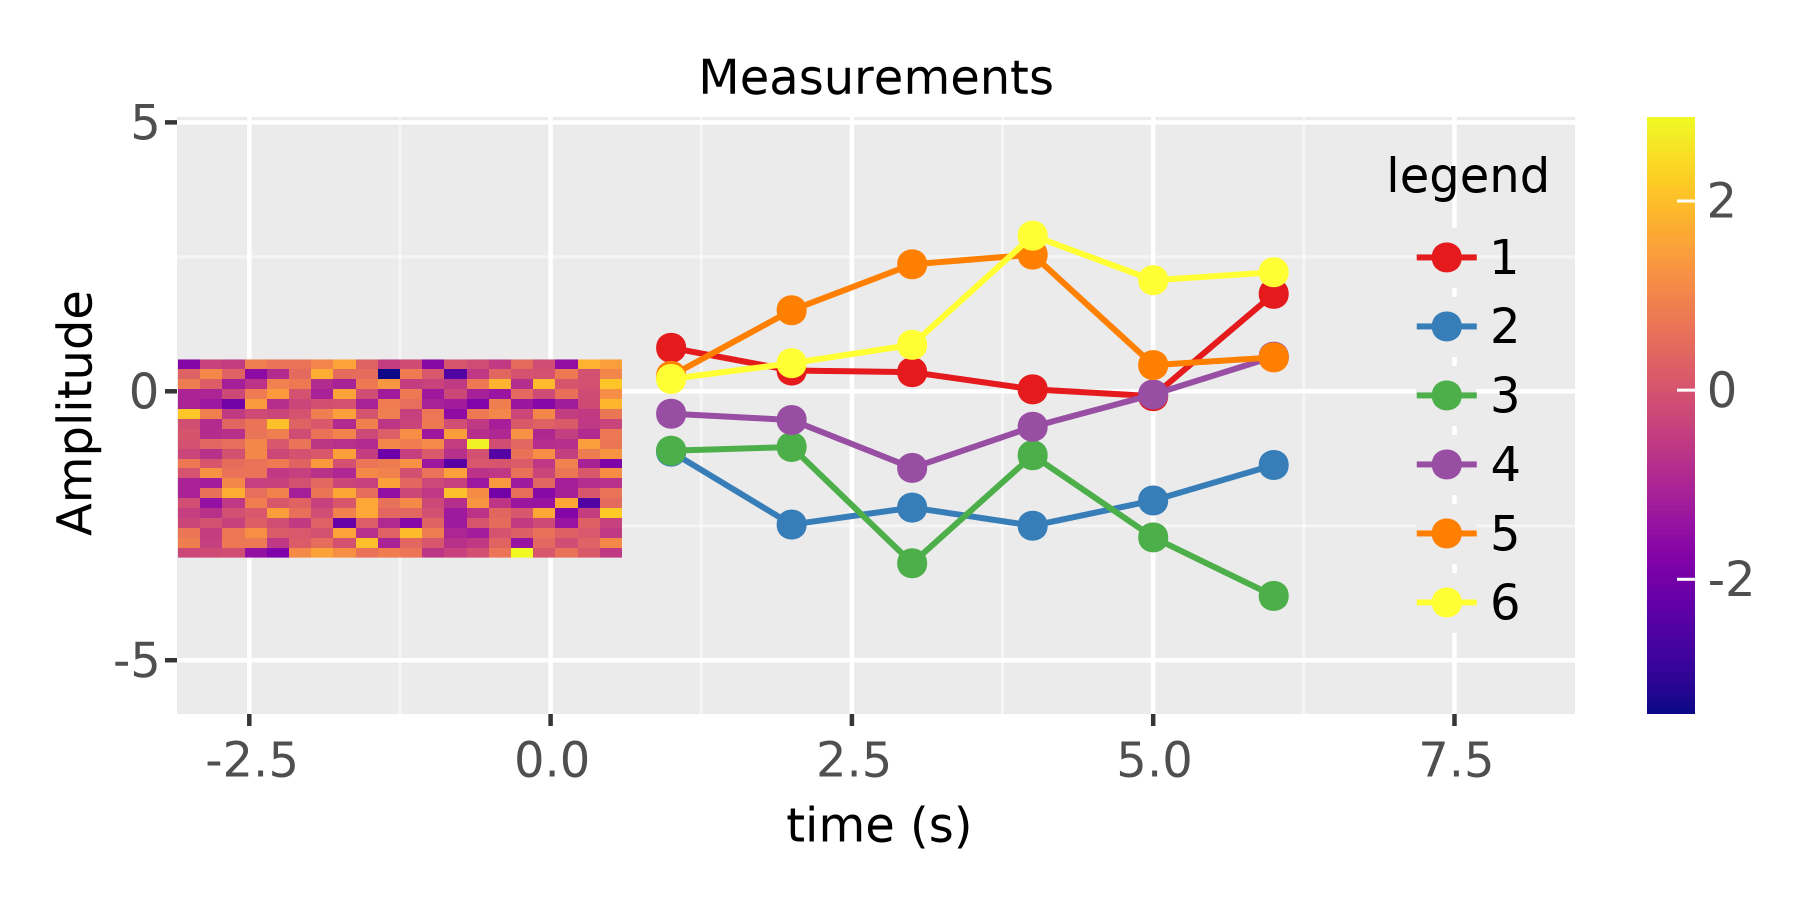
\includegraphics[width=0.6\textwidth,height=\textheight]{_build/im/theme_ggplot2.png}
\caption{Theme ggplot2.}\label{fig:theme_ggplot2}
}
\end{figure}

\begin{figure}
\hypertarget{fig:theme_minimal}{%
\centering
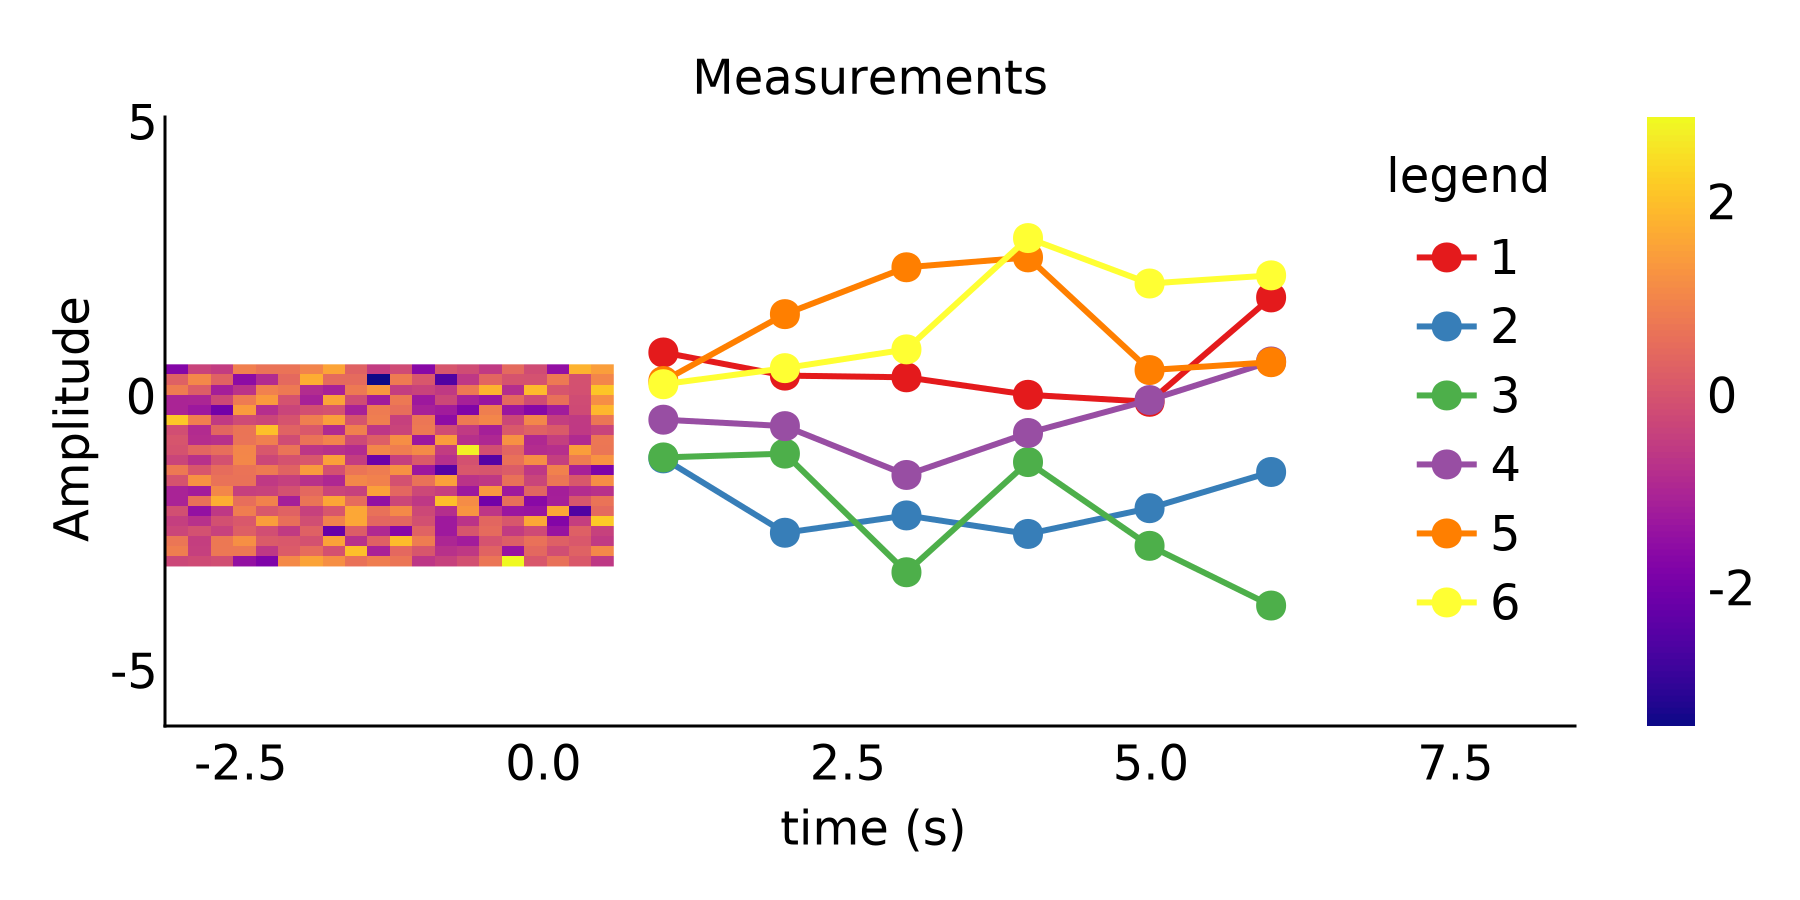
\includegraphics[width=0.6\textwidth,height=\textheight]{_build/im/theme_minimal.png}
\caption{Theme minimal.}\label{fig:theme_minimal}
}
\end{figure}

\begin{figure}
\hypertarget{fig:theme_light}{%
\centering
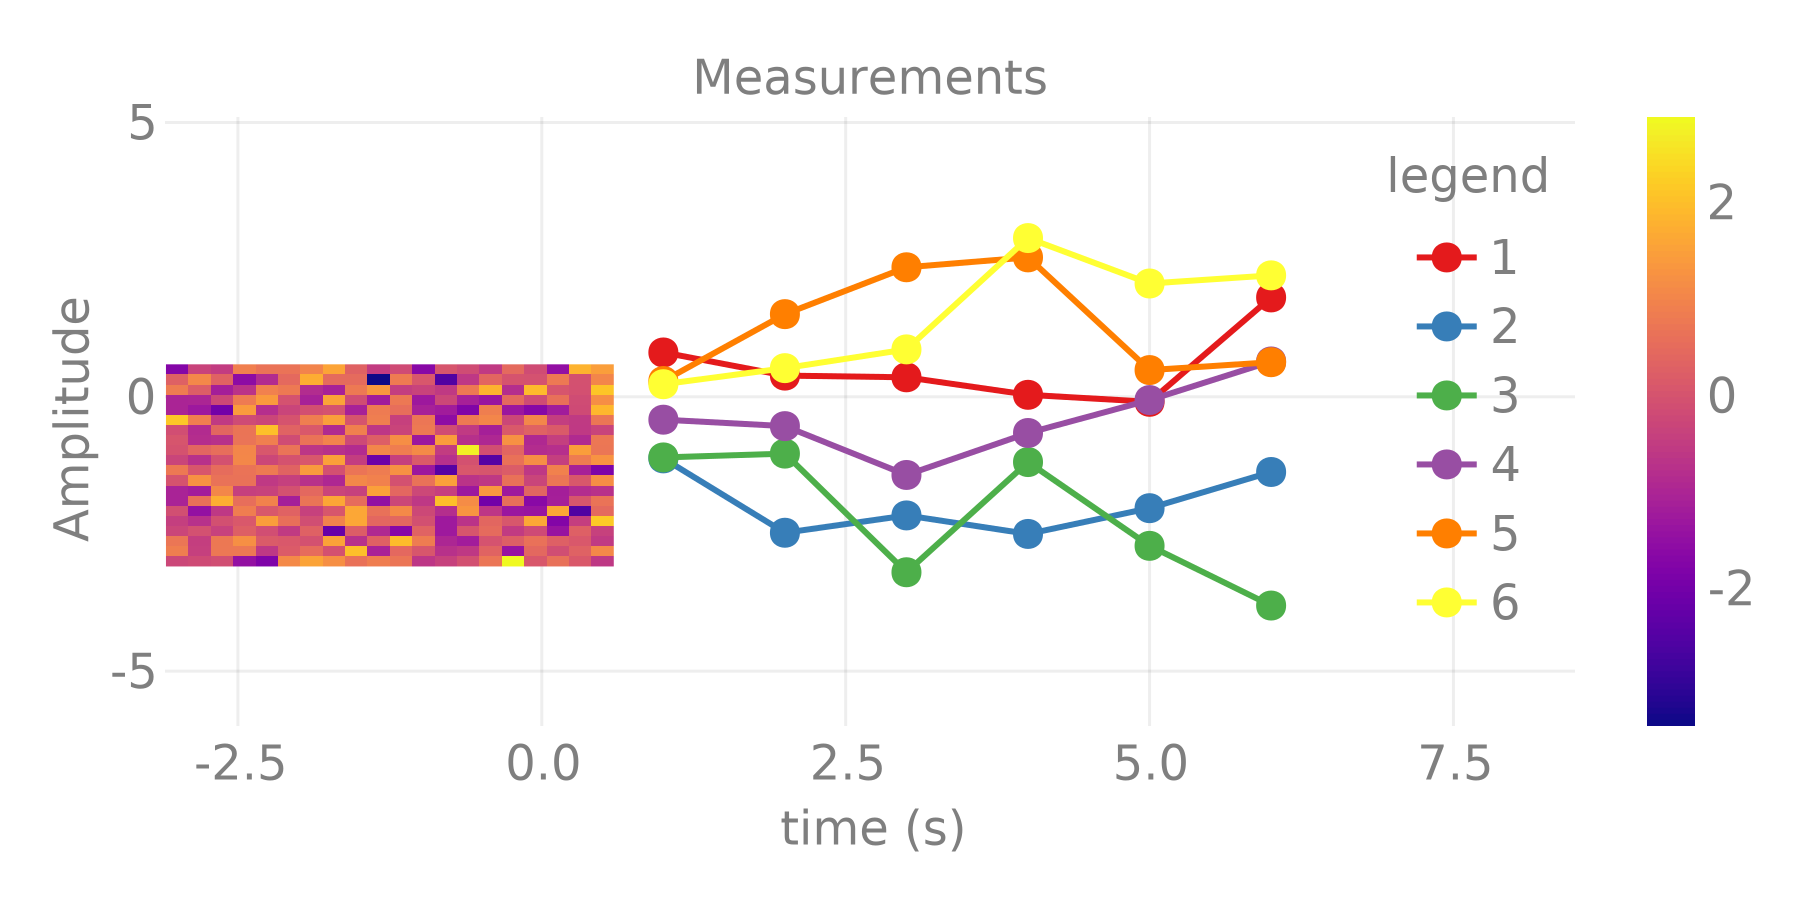
\includegraphics[width=0.6\textwidth,height=\textheight]{_build/im/theme_light.png}
\caption{Theme light.}\label{fig:theme_light}
}
\end{figure}

另一种方案是通过使用
\passthrough{\lstinline!with\_theme(your\_plot, your\_theme())!}
创建自定义 \passthrough{\lstinline!Theme!} 。
例如,以下主题可以作为出版质量图的初级模板:

\begin{lstlisting}[language=Julia]
publication_theme() = Theme(
    fontsize=16, font="CMU Serif",
    Axis=(xlabelsize=20, xgridstyle=:dash, ygridstyle=:dash,
        xtickalign=1, ytickalign=1, yticksize=10, xticksize=10,
        xlabelpadding=-5, xlabel="x", ylabel="y"),
    Legend=(framecolor=(:black, 0.5), bgcolor=(:white, 0.5)),
    Colorbar=(ticksize=16, tickalign=1, spinewidth=0.5),
)
\end{lstlisting}

为简单起见,在接下来的例子中使用它绘制
\passthrough{\lstinline!scatterlines!} 和
\passthrough{\lstinline!heatmap!}。

\begin{lstlisting}[language=Julia]
function plot_with_legend_and_colorbar()
    fig, ax, _ = scatterlines(1:10; label="line")
    hm = heatmap!(ax, LinRange(6, 9, 15), LinRange(2, 5, 15), randn(15, 15);
        colormap=:Spectral_11)
    axislegend("legend"; position=:lt)
    Colorbar(fig[1, 2], hm, label="values")
    ax.title = "my custom theme"
    fig
end
\end{lstlisting}

然后使用前面定义的 \passthrough{\lstinline!Theme!},其输出如
(图~\ref{fig:plot_with_legend_and_colorbar}) 所示。

\begin{lstlisting}[language=Julia]
with_theme(plot_with_legend_and_colorbar, publication_theme())
\end{lstlisting}

\begin{figure}
\hypertarget{fig:plot_with_legend_and_colorbar}{%
\centering
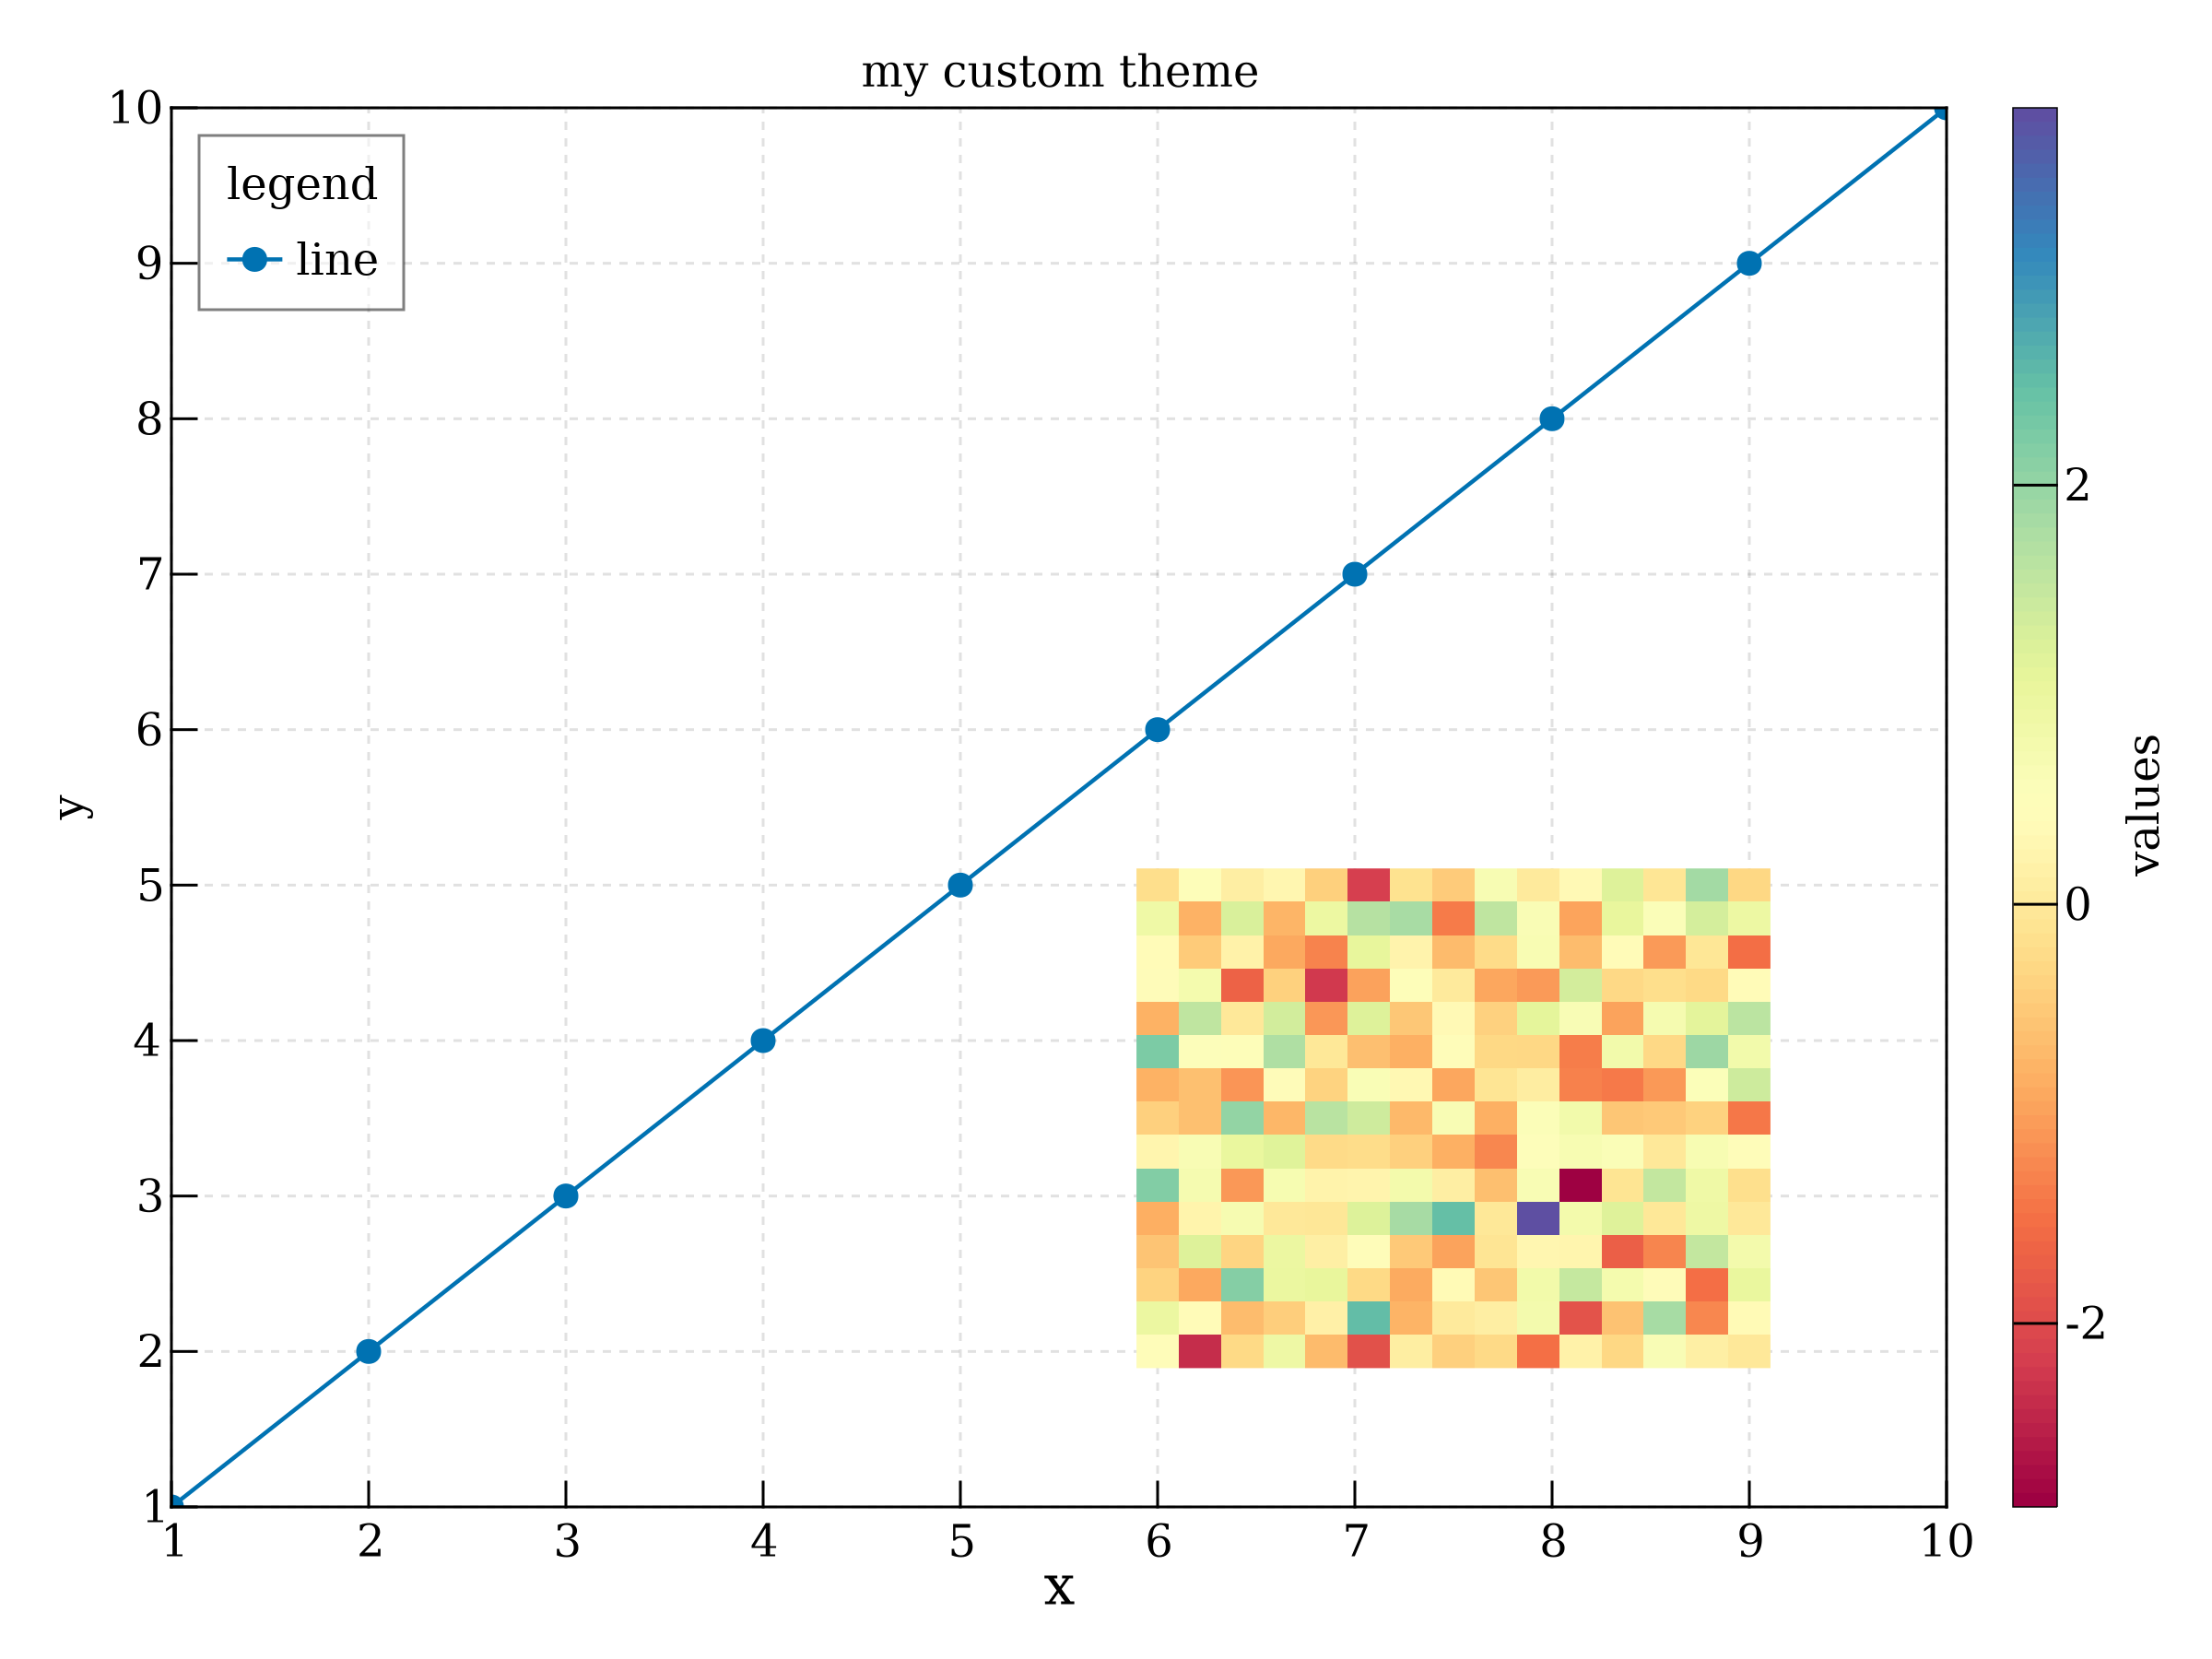
\includegraphics[width=0.6\textwidth,height=\textheight]{_build/im/plot_with_legend_and_colorbar.png}
\caption{Themed plot with Legend and
Colorbar.}\label{fig:plot_with_legend_and_colorbar}
}
\end{figure}

如果需要在
\passthrough{\lstinline"set\_theme!(your\_theme)"}后更改一些设置,那么可以使用
\passthrough{\lstinline"update\_theme!(resolution=(500, 400), fontsize=18)"}。
另一种方法是给 \passthrough{\lstinline!with\_theme!}
函数传递额外的参数:

\begin{lstlisting}[language=Julia]
fig = (resolution=(600, 400), figure_padding=1, backgroundcolor=:grey90)
ax = (; aspect=DataAspect(), xlabel=L"x", ylabel=L"y")
cbar = (; height=Relative(4 / 5))
with_theme(publication_theme(); fig..., Axis=ax, Colorbar=cbar) do
    plot_with_legend_and_colorbar()
end
\end{lstlisting}

\begin{figure}
\hypertarget{fig:plot_theme_extra_args}{%
\centering
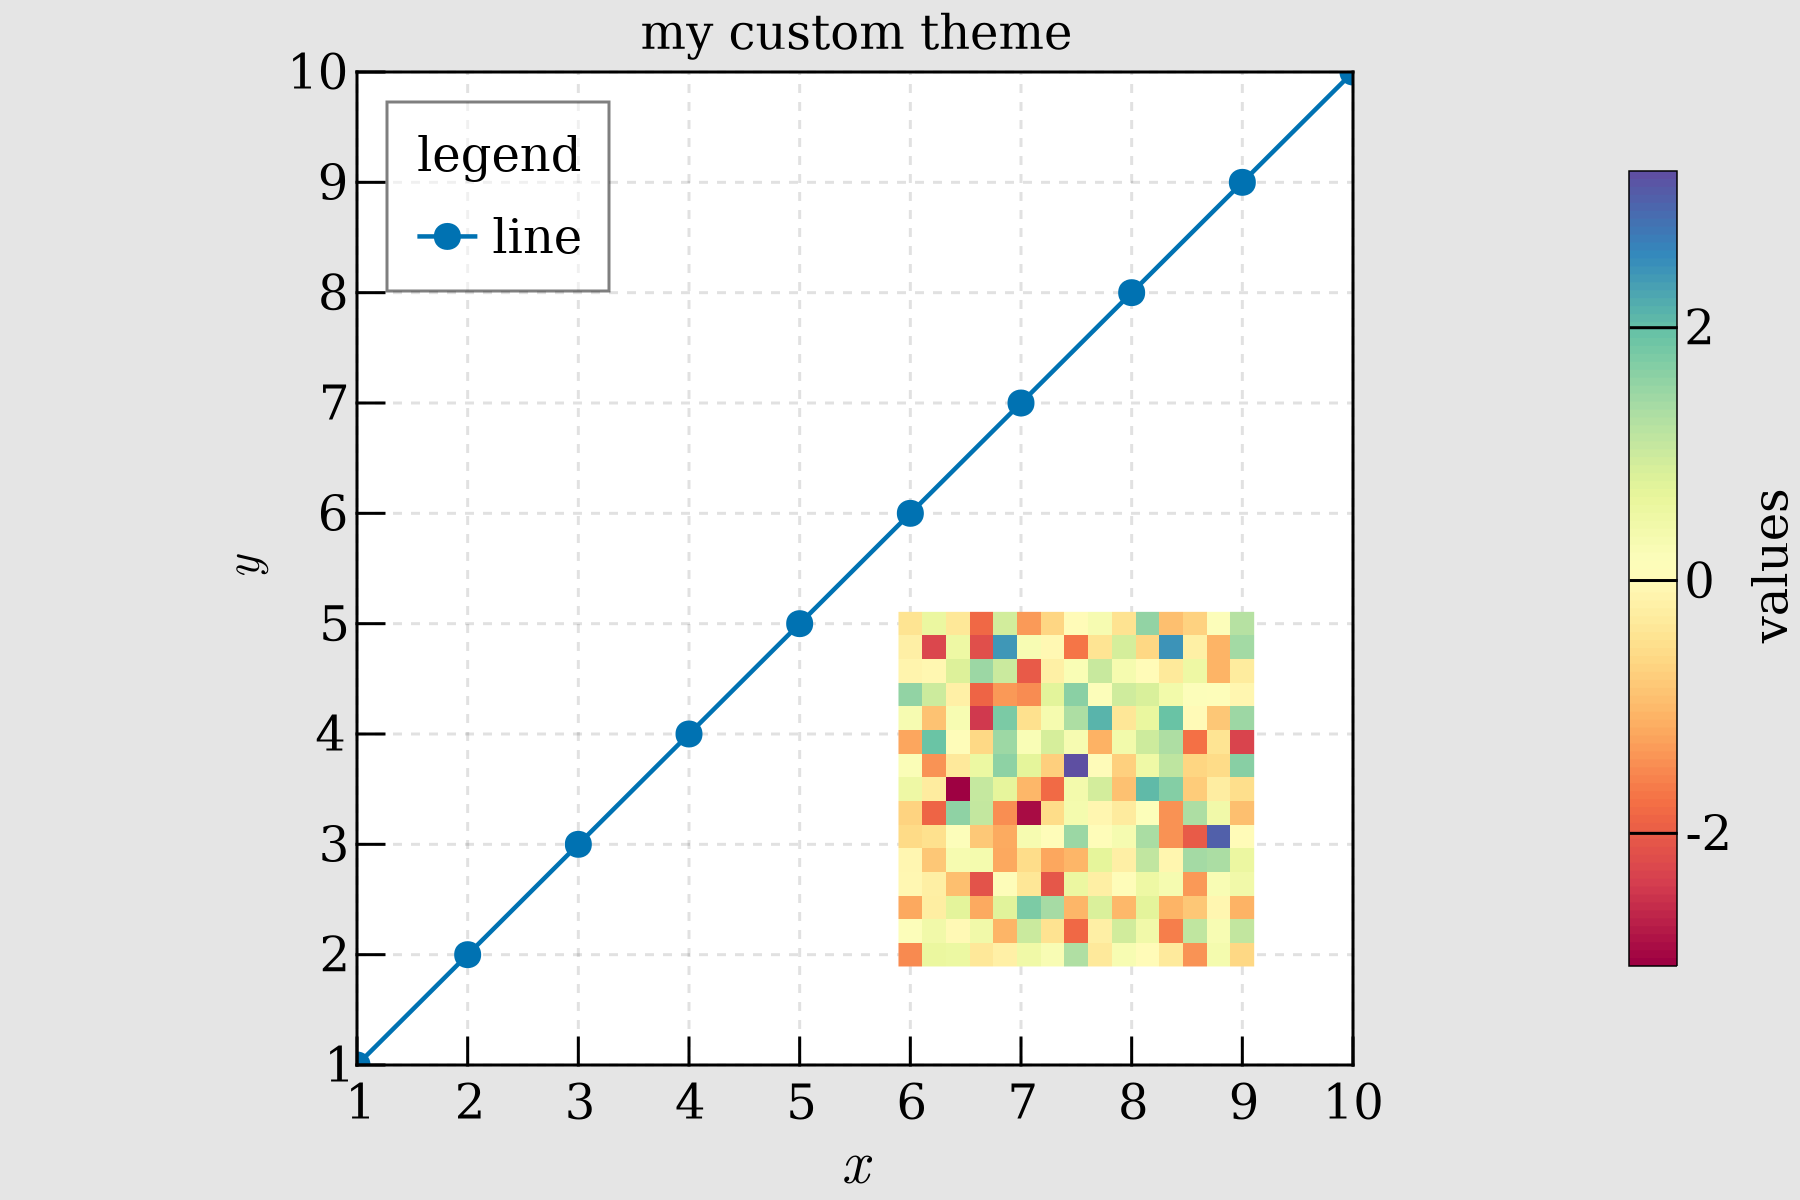
\includegraphics[width=0.6\textwidth,height=\textheight]{_build/im/plot_theme_extra_args.png}
\caption{Theme with extra args.}\label{fig:plot_theme_extra_args}
}
\end{figure}

现在,接下来将讨论如何使用 LaTeX 字符串和自定义主题进行绘图。

\hypertarget{sec:using_latex}{%
\section{使用 LaTeXStrings.jl}\label{sec:using_latex}}

通过调用
\passthrough{\lstinline!LaTeXStrings.jl!},\passthrough{\lstinline!Makie.jl!}
实现了对 LaTeX 的支持:

\begin{lstlisting}
using LaTeXStrings
\end{lstlisting}

一个简单的基础用法例子如下所示
(图~\ref{fig:latex_strings}),其主要包含用于 x-y 标签和图例的 LaTeX
字符串。

\begin{lstlisting}[language=Julia]
function LaTeX_Strings()
    x = 0:0.05:4π
    lines(x, x -> sin(3x) / (cos(x) + 2) / x; label=L"\frac{\sin(3x)}{x(\cos(x)+2)}",
        figure=(; resolution=(600, 400)), axis=(; xlabel=L"x"))
    lines!(x, x -> cos(x) / x; label=L"\cos(x)/x")
    lines!(x, x -> exp(-x); label=L"e^{-x}")
    limits!(-0.5, 13, -0.6, 1.05)
    axislegend(L"f(x)")
    current_figure()
end
\end{lstlisting}

\begin{lstlisting}[language=Julia]
with_theme(LaTeX_Strings, publication_theme())
\end{lstlisting}

\begin{figure}
\hypertarget{fig:latex_strings}{%
\centering
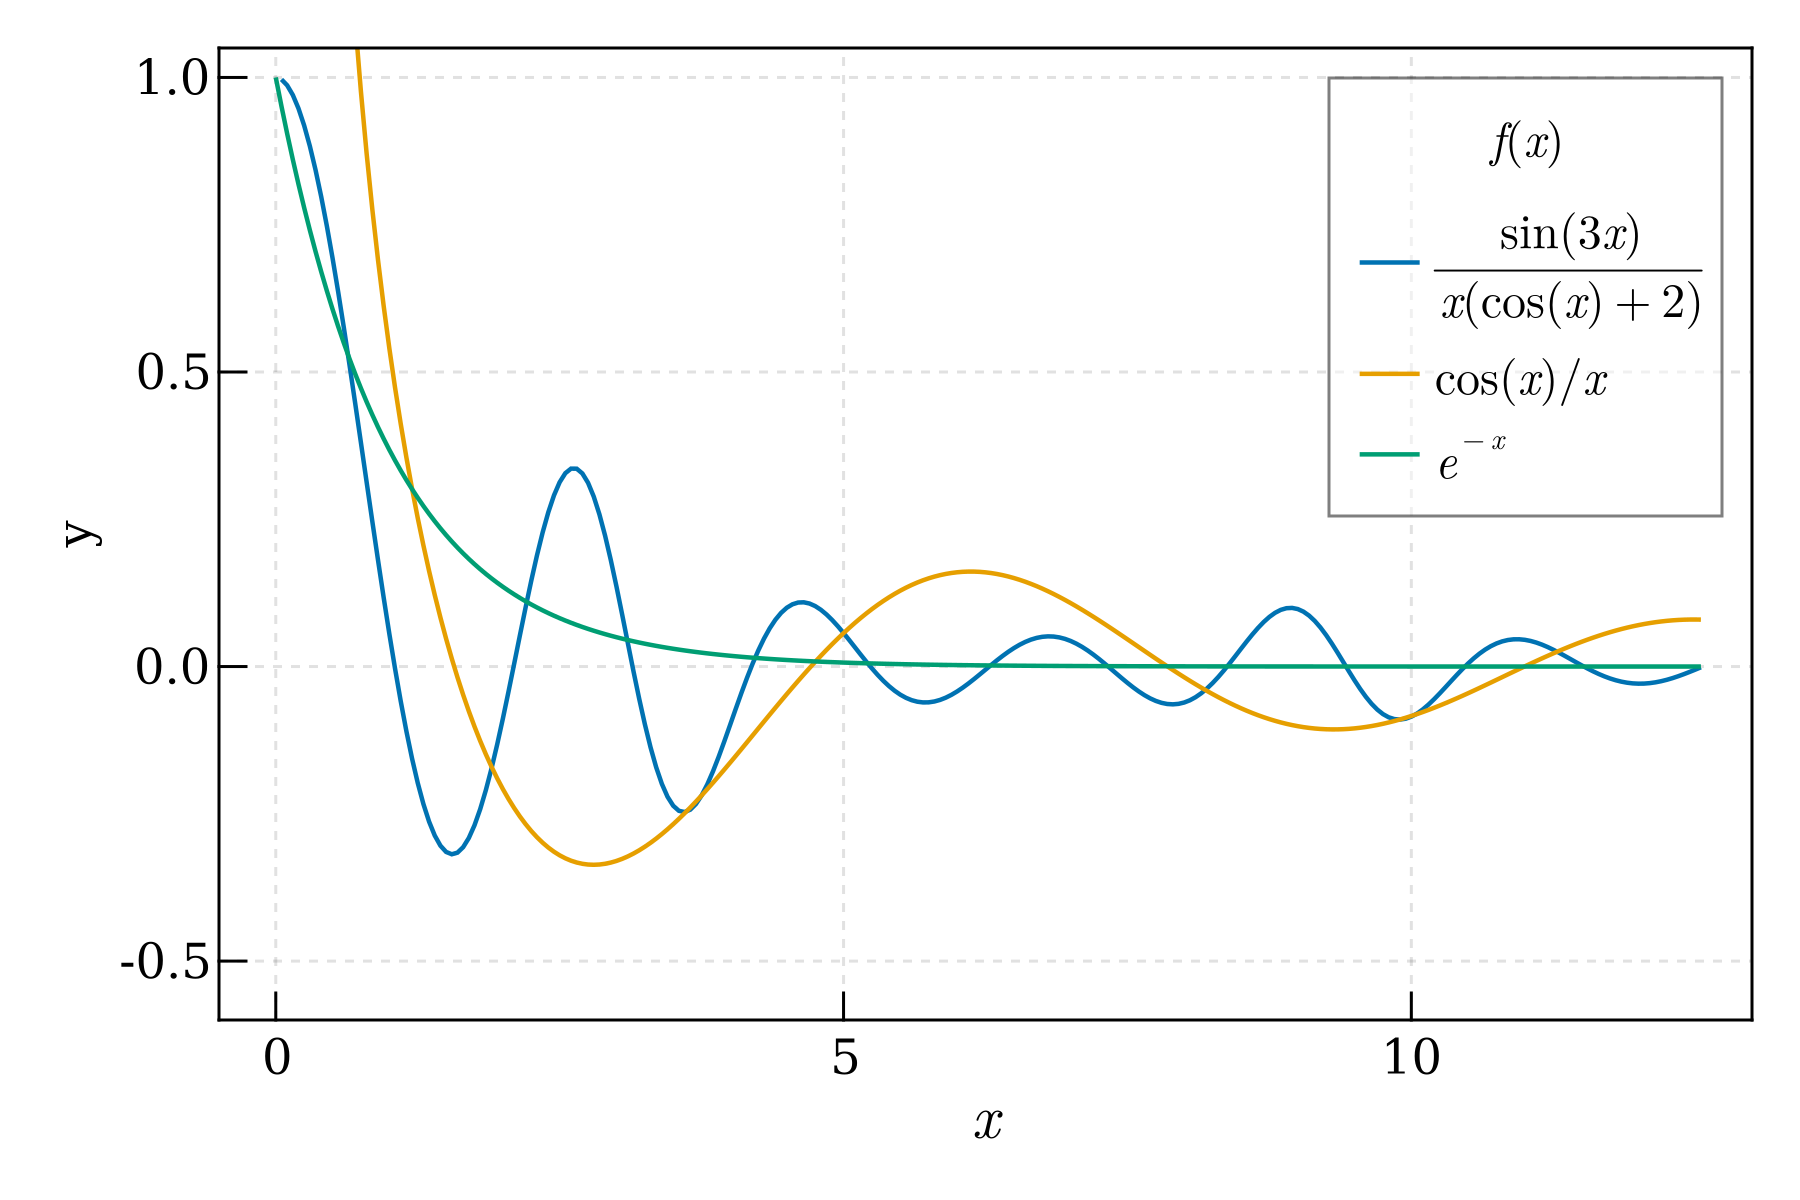
\includegraphics[width=0.6\textwidth,height=\textheight]{_build/im/latex_strings.png}
\caption{Plot with LaTeX strings.}\label{fig:latex_strings}
}
\end{figure}

下面是更复杂的例子,图中的\passthrough{\lstinline!text!}是一些等式,并且图例编号随着曲线数增加:

\begin{lstlisting}[language=Julia]
function multiple_lines()
    x = collect(0:10)
    fig = Figure(resolution=(600, 400), font="CMU Serif")
    ax = Axis(fig[1, 1], xlabel=L"x", ylabel=L"f(x,a)")
    for i = 0:10
        lines!(ax, x, i .* x; label=latexstring("$(i) x"))
    end
    axislegend(L"f(x)"; position=:lt, nbanks=2, labelsize=14)
    text!(L"f(x,a) = ax", position=(4, 80))
    fig
end
multiple_lines()
\end{lstlisting}

\begin{figure}
\hypertarget{fig:multiple_lines}{%
\centering
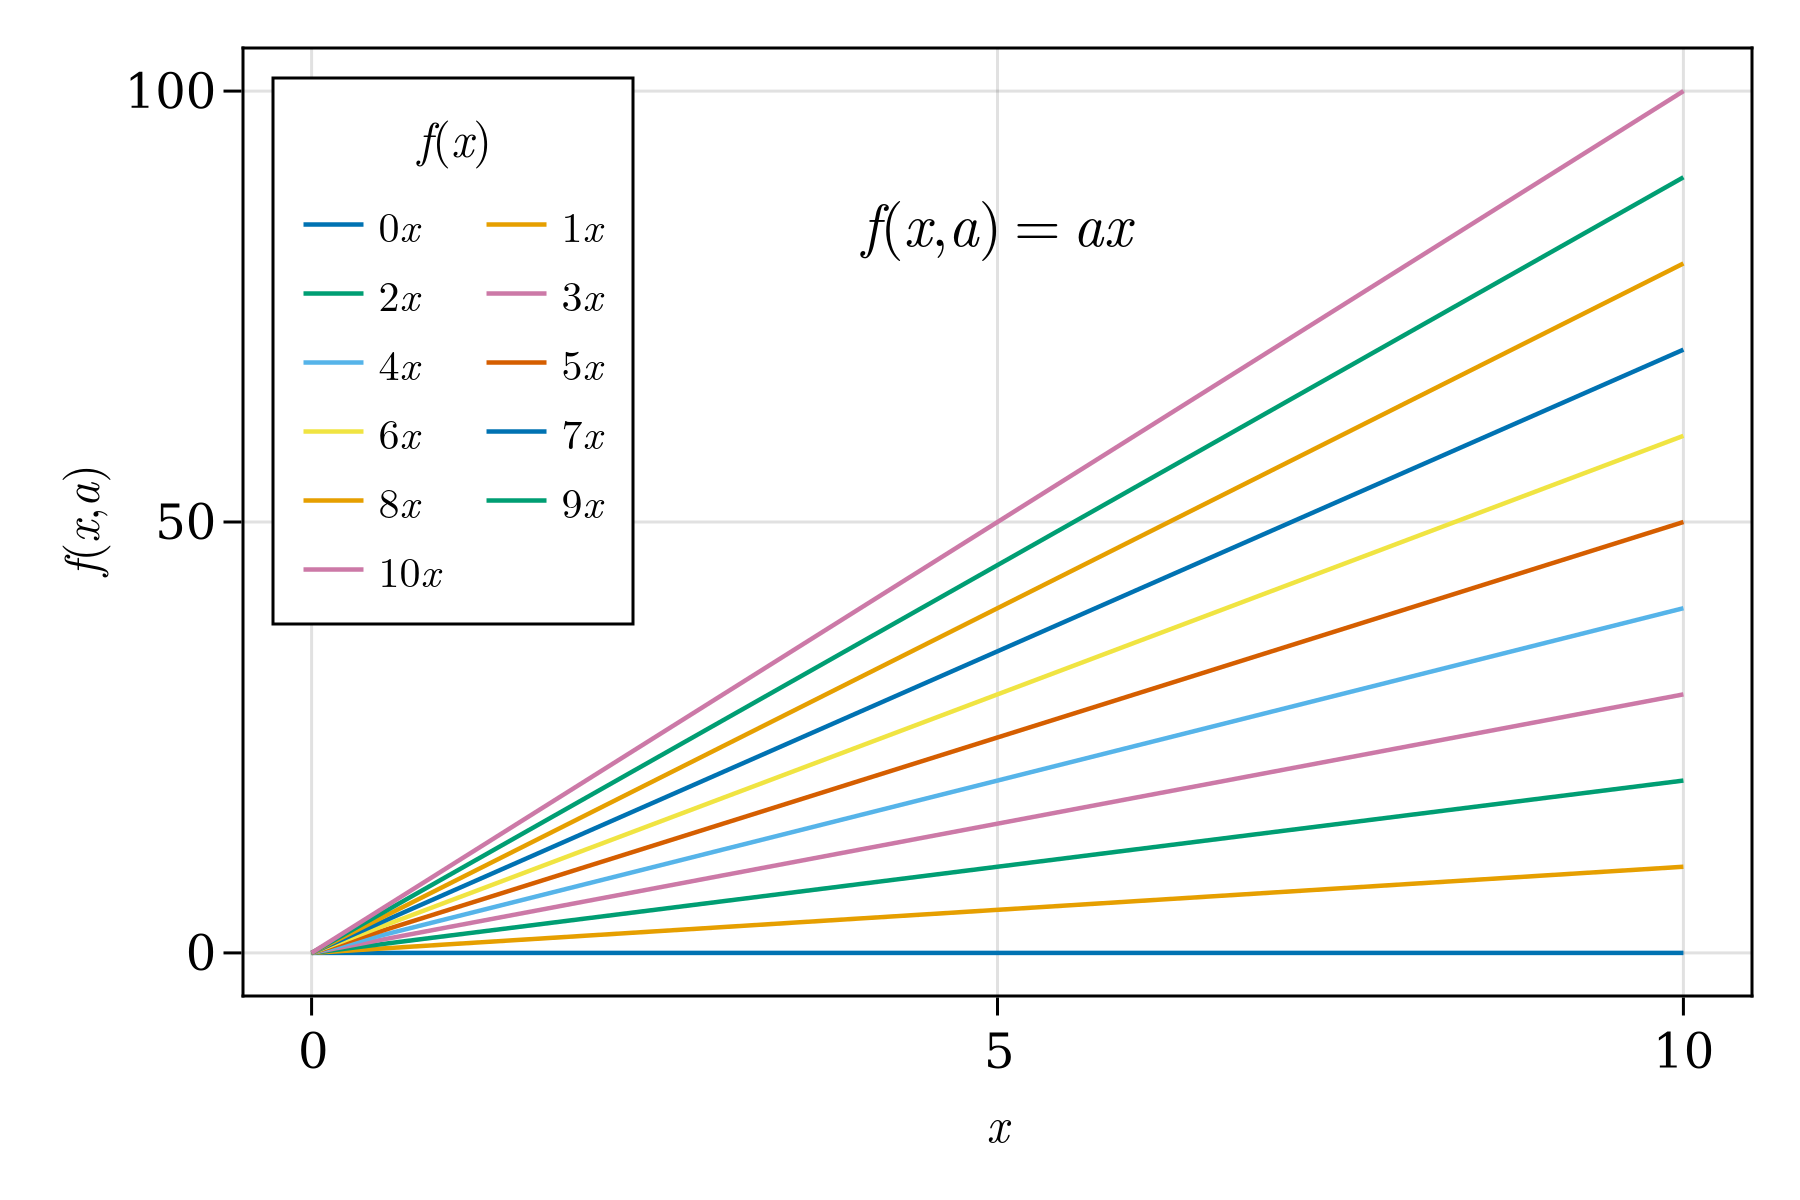
\includegraphics[width=0.6\textwidth,height=\textheight]{_build/im/JDS_multiple_lines_.png}
\caption{Multiple lines.}\label{fig:multiple_lines}
}
\end{figure}

但不太好的是,一些曲线的颜色是重复的。
添加标记和线条类型通常能解决此问题。 所以让我们使用
\href{http://makie.juliaplots.org/stable/documentation/theming/index.html\#cycles}{\passthrough{\lstinline!Cycles!}}
来添加标记和线条类型。 设置
\passthrough{\lstinline!covary=true!},使所有元素一起循环:

\begin{lstlisting}[language=Julia]
function multiple_scatters_and_lines()
    x = collect(0:10)
    cycle = Cycle([:color, :linestyle, :marker], covary=true)
    set_theme!(Lines=(cycle=cycle,), Scatter=(cycle=cycle,))
    fig = Figure(resolution=(600, 400), font="CMU Serif")
    ax = Axis(fig[1, 1], xlabel=L"x", ylabel=L"f(x,a)")
    for i in x
        lines!(ax, x, i .* x; label=latexstring("$(i) x"))
        scatter!(ax, x, i .* x; markersize=13, strokewidth=0.25,
            label=latexstring("$(i) x"))
    end
    axislegend(L"f(x)"; merge=true, position=:lt, nbanks=2, labelsize=14)
    text!(L"f(x,a) = ax", position=(4, 80))
    set_theme!() # reset to default theme
    fig
end
multiple_scatters_and_lines()
\end{lstlisting}

\begin{figure}
\hypertarget{fig:multiple_scatters_and_lines}{%
\centering
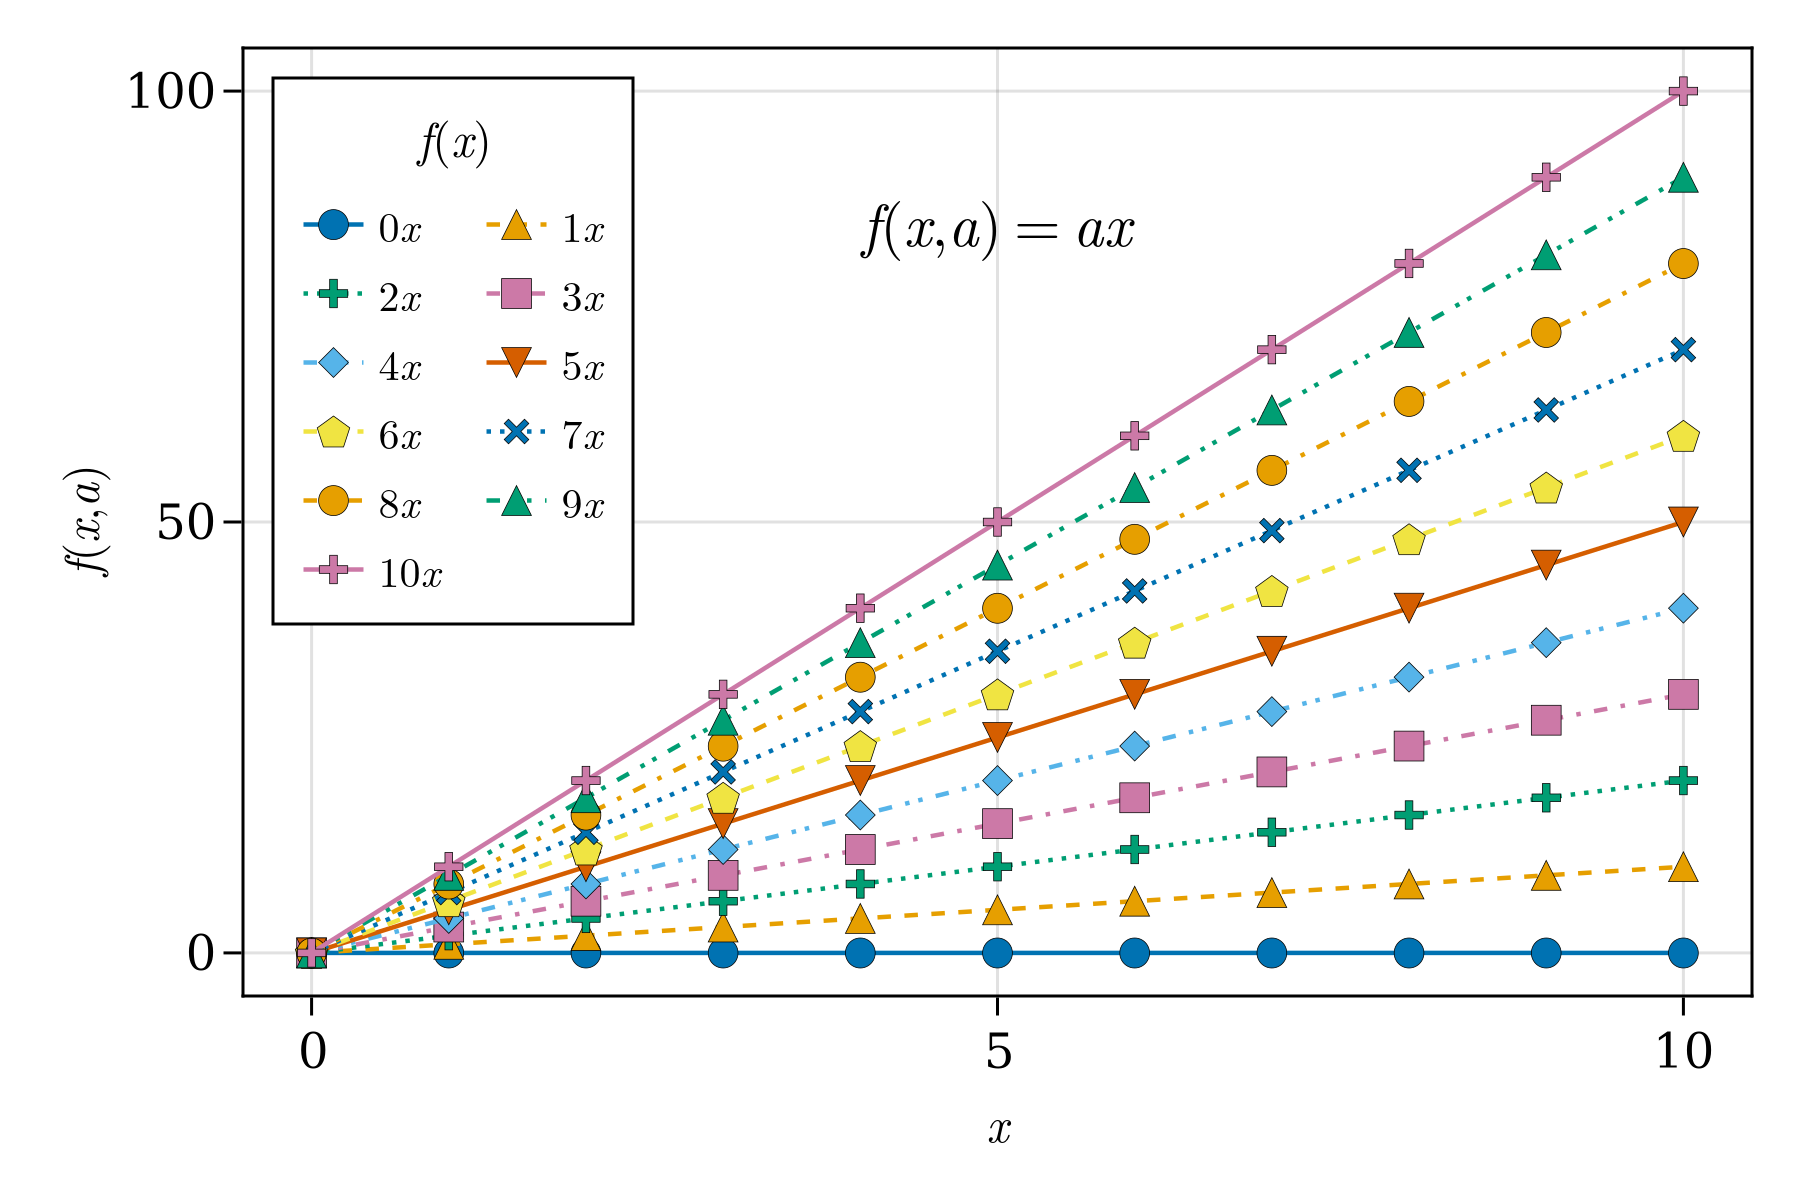
\includegraphics[width=0.6\textwidth,height=\textheight]{_build/im/JDS_multiple_scatters_and_lines_.png}
\caption{Multiple Scatters and
Lines.}\label{fig:multiple_scatters_and_lines}
}
\end{figure}

一张出版质量的图如上所示。 那我们还能做些什么操作?
答案是还可以为图定义不同的默认颜色或者调色盘。
在下一节,我们将再次了解如何使用
\href{http://makie.juliaplots.org/stable/documentation/theming/index.html\#cycles}{\passthrough{\lstinline!Cycles!}}
以及有关它的更多信息,即通过添加额外的关键字参数就可以实现前面的操作。

\hypertarget{sec:makie_colors}{%
\section{颜色和颜色图(Colormap)}\label{sec:makie_colors}}

在展示结果时,其中重要的一步是为图选择一组合适的颜色或 colorbar。
\passthrough{\lstinline!Makie.jl!} 支持使用
\href{https://github.com/JuliaGraphics/Colors.jl}{Colors.jl}
,因此你可以使用
\href{https://juliagraphics.github.io/Colors.jl/latest/namedcolors/}{named
colors} 而不是传递 \passthrough{\lstinline!RGB!} 或
\passthrough{\lstinline!RGBA!} 值。 另外,也可以使用
\href{https://github.com/JuliaGraphics/ColorSchemes.jl}{ColorSchemes.jl}
和
\href{https://github.com/peterkovesi/PerceptualColourMaps.jl}{PerceptualColourMaps.jl}
中的颜色图。 值得了解的是,可以使用
\passthrough{\lstinline!Reverse(:colormap\_name)!} 反转颜色图
,也可以通过 \passthrough{\lstinline!color=(:red,0.5)!} and
\passthrough{\lstinline!colormap=(:viridis, 0.5)!}
获得透明的颜色或颜色图。

下文介绍不同的用例。
接下来使用新的颜色和颜色栏(Colorbar)调色盘来创建自定义主题。

默认情况下, \passthrough{\lstinline!Makie.jl!}
已经预定义一组颜色,可以循环使用该组颜色。
之前的图因此并未设置任何特定颜色。
覆盖这些默认颜色的方法是,在绘图函数中调用
\passthrough{\lstinline!color!} 关键字并使用
\passthrough{\lstinline!Symbol!} 或 \passthrough{\lstinline!String!}
指定新的颜色。 该操作如下所示:

\begin{lstlisting}[language=Julia]
function set_colors_and_cycle()
    # Epicycloid lines
    x(r, k, θ) = r * (k .+ 1.0) .* cos.(θ) .- r * cos.((k .+ 1.0) .* θ)
    y(r, k, θ) = r * (k .+ 1.0) .* sin.(θ) .- r * sin.((k .+ 1.0) .* θ)
    θ = LinRange(0, 6.2π, 1000)
    axis = (; xlabel=L"x(\theta)", ylabel=L"y(\theta)",
        title="Epicycloid", aspect=DataAspect())
    figure = (; resolution=(600, 400), font="CMU Serif")
    fig, ax, _ = lines(x(1, 1, θ), y(1, 1, θ); color="firebrick1", # string
        label=L"1.0", axis=axis, figure=figure)
    lines!(ax, x(4, 2, θ), y(4, 2, θ); color=:royalblue1, #symbol
        label=L"2.0")
    for k = 2.5:0.5:5.5
        lines!(ax, x(2k, k, θ), y(2k, k, θ); label=latexstring("$(k)")) #cycle
    end
    Legend(fig[1, 2], ax, latexstring("k, r = 2k"), merge=true)
    fig
end
set_colors_and_cycle()
\end{lstlisting}

\begin{figure}
\hypertarget{fig:set_colors_and_cycle}{%
\centering
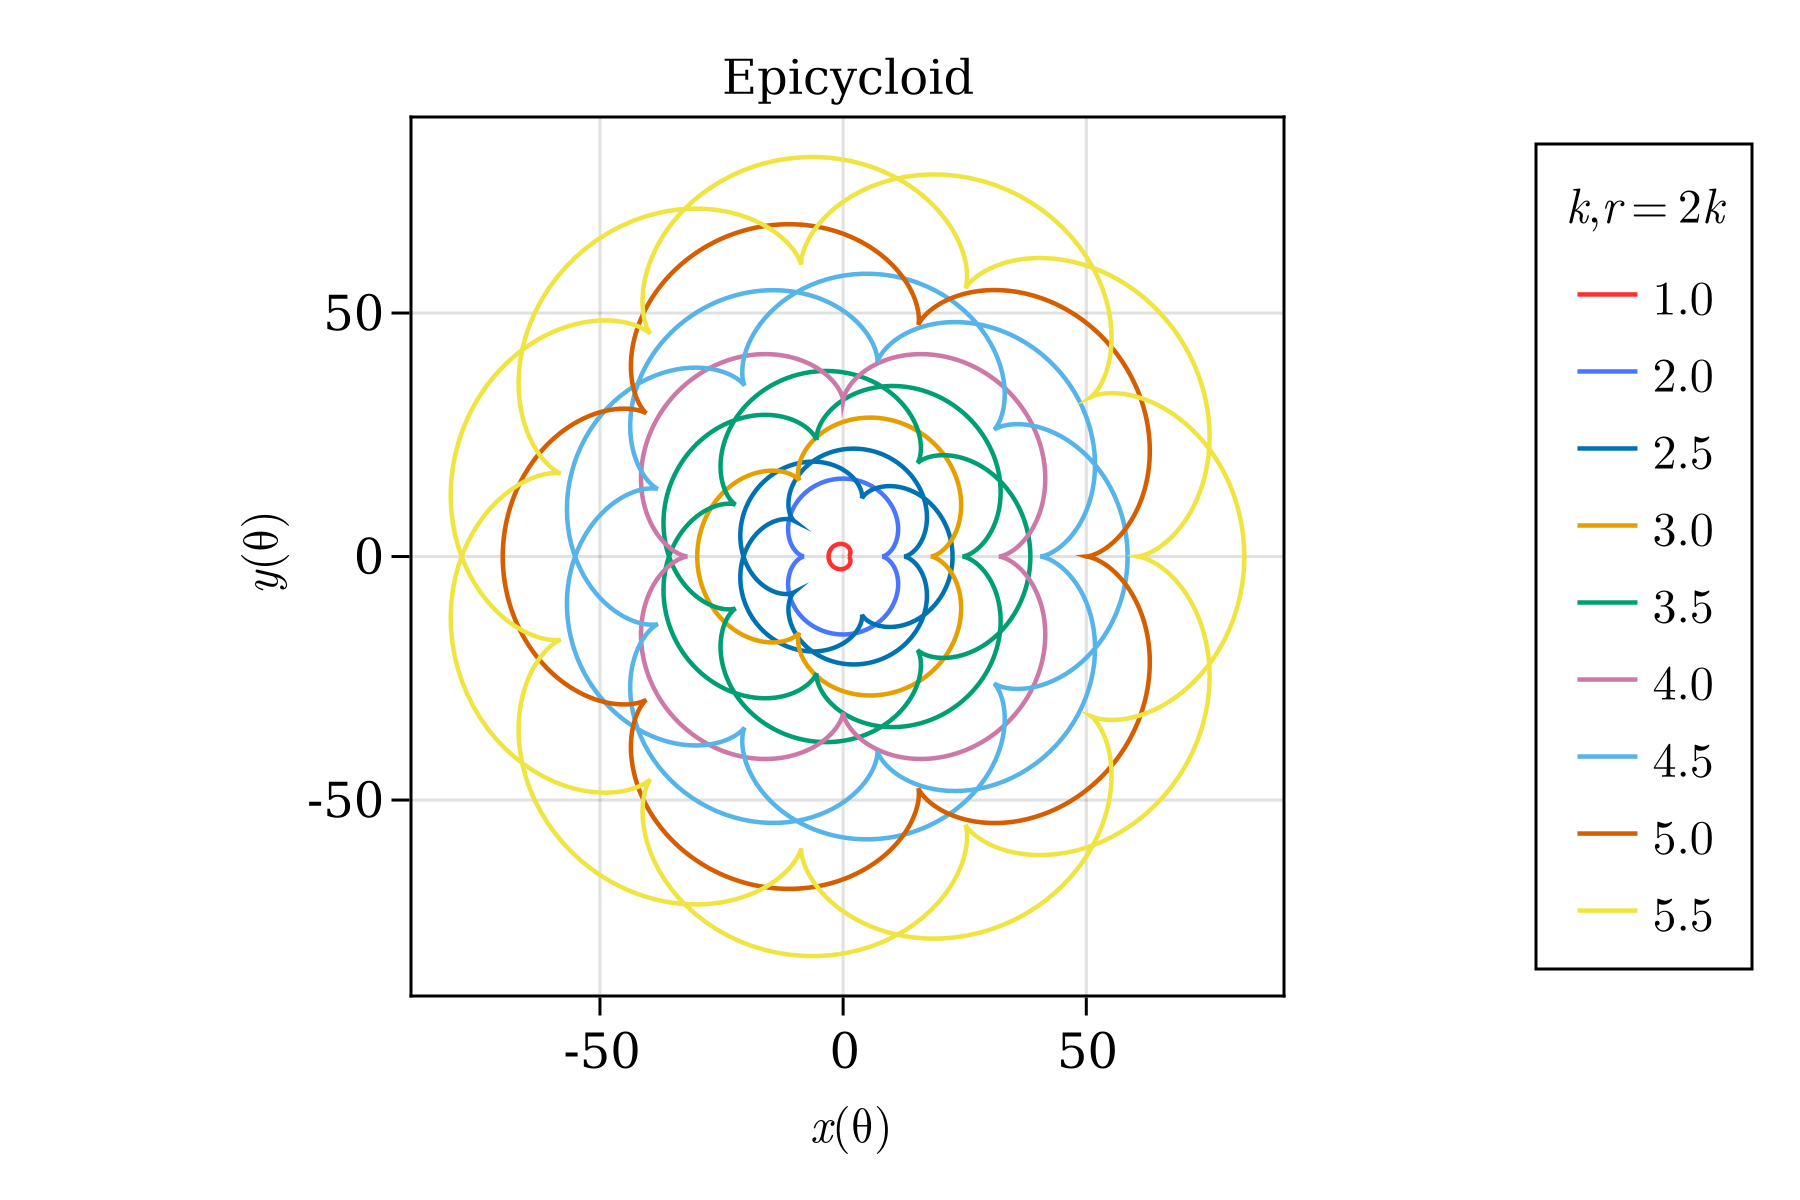
\includegraphics{_build/im/JDS_set_colors_and_cycle_.png}
\caption{Set colors and cycle.}\label{fig:set_colors_and_cycle}
}
\end{figure}

这里通过\passthrough{\lstinline!color!}
关键字指定了上例前两条曲线的颜色。 其余使用默认的颜色集。
稍后将学习如何使用自定义颜色循环。

关于颜色图,我们已经非常熟悉用于热力图和散点图的
\passthrough{\lstinline!colormap!}。下面展示的是,颜色图也可以像颜色那样通过
\passthrough{\lstinline!Symbol!} 或 \passthrough{\lstinline!String!}
进行指定。 此外,也可以是 \passthrough{\lstinline!RGB!} 颜色的向量。
下面是第一个例子,通过 \passthrough{\lstinline!Symbol!},
\passthrough{\lstinline!String!} 和分类值的
\passthrough{\lstinline!cgrad!} 来指定颜色图。 输入
\passthrough{\lstinline!?cgrad!} 查看更多信息。

\begin{lstlisting}[language=Julia]
figure = (; resolution=(600, 400), font="CMU Serif")
axis = (; xlabel=L"x", ylabel=L"y", aspect=DataAspect())
fig, ax, pltobj = heatmap(rand(20, 20); colorrange=(0, 1),
    colormap=Reverse(:viridis), axis=axis, figure=figure)
Colorbar(fig[1, 2], pltobj, label = "Reverse colormap Sequential")
fig
\end{lstlisting}

\begin{figure}
\hypertarget{fig:Reverse_colormap_sequential}{%
\centering
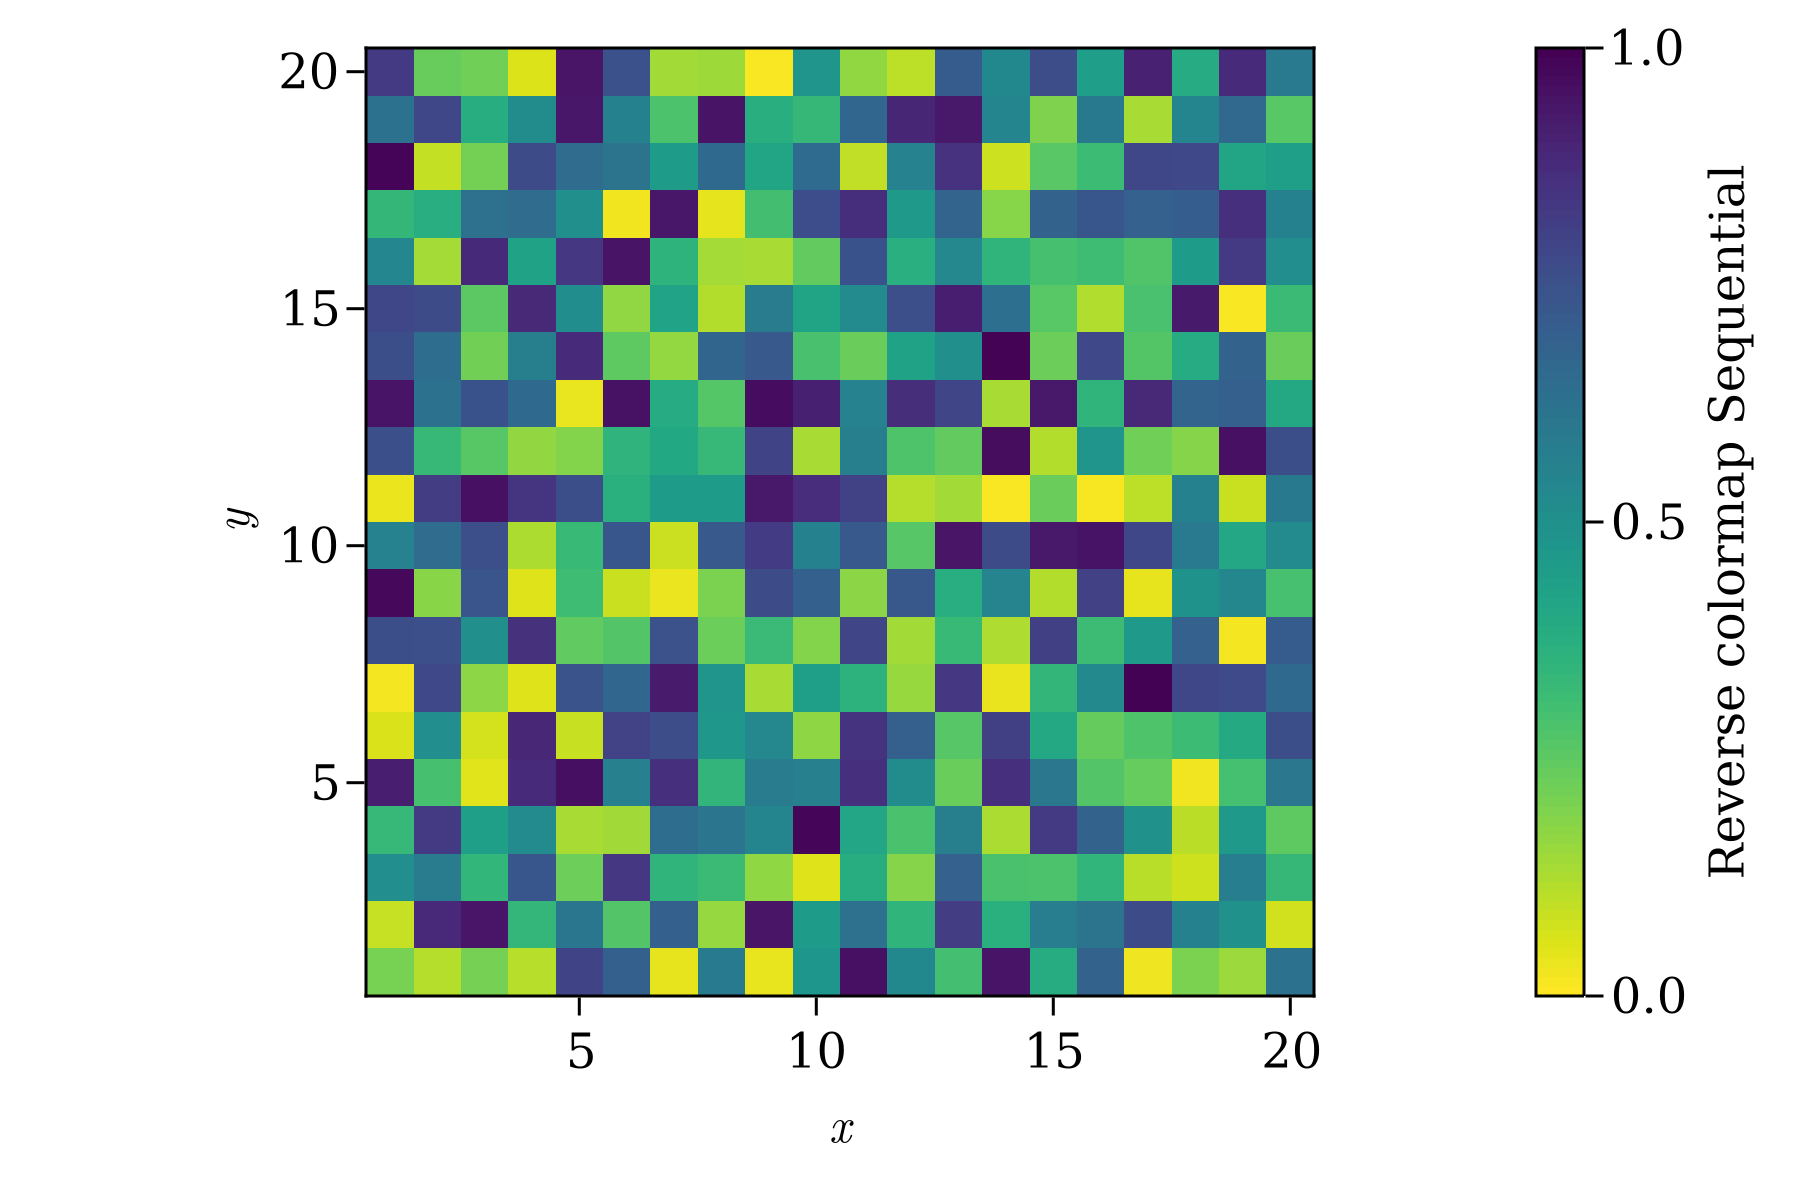
\includegraphics[width=0.6\textwidth,height=\textheight]{_build/im/Reverse_colormap_sequential.png}
\caption{Reverse colormap sequential and
colorrange.}\label{fig:Reverse_colormap_sequential}
}
\end{figure}

当设置 \passthrough{\lstinline!colorrange!}
后,超出此范围的颜色值会被相应地设置为颜色图的第一种和最后一种颜色。
但是,有时最好自行指定两端的颜色。这可以通过
\passthrough{\lstinline!highclip!} 和 \passthrough{\lstinline!lowclip!}
实现:

\begin{lstlisting}
using ColorSchemes
\end{lstlisting}

\begin{lstlisting}[language=Julia]
figure = (; resolution=(600, 400), font="CMU Serif")
axis = (; xlabel=L"x", ylabel=L"y", aspect=DataAspect())
fig, ax, pltobj=heatmap(randn(20, 20); colorrange=(-2, 2),
    colormap="diverging_rainbow_bgymr_45_85_c67_n256",
    highclip=:black, lowclip=:white, axis=axis, figure=figure)
Colorbar(fig[1, 2], pltobj, label = "Diverging colormap")
fig
\end{lstlisting}

\begin{figure}
\hypertarget{fig:diverging_colormap}{%
\centering
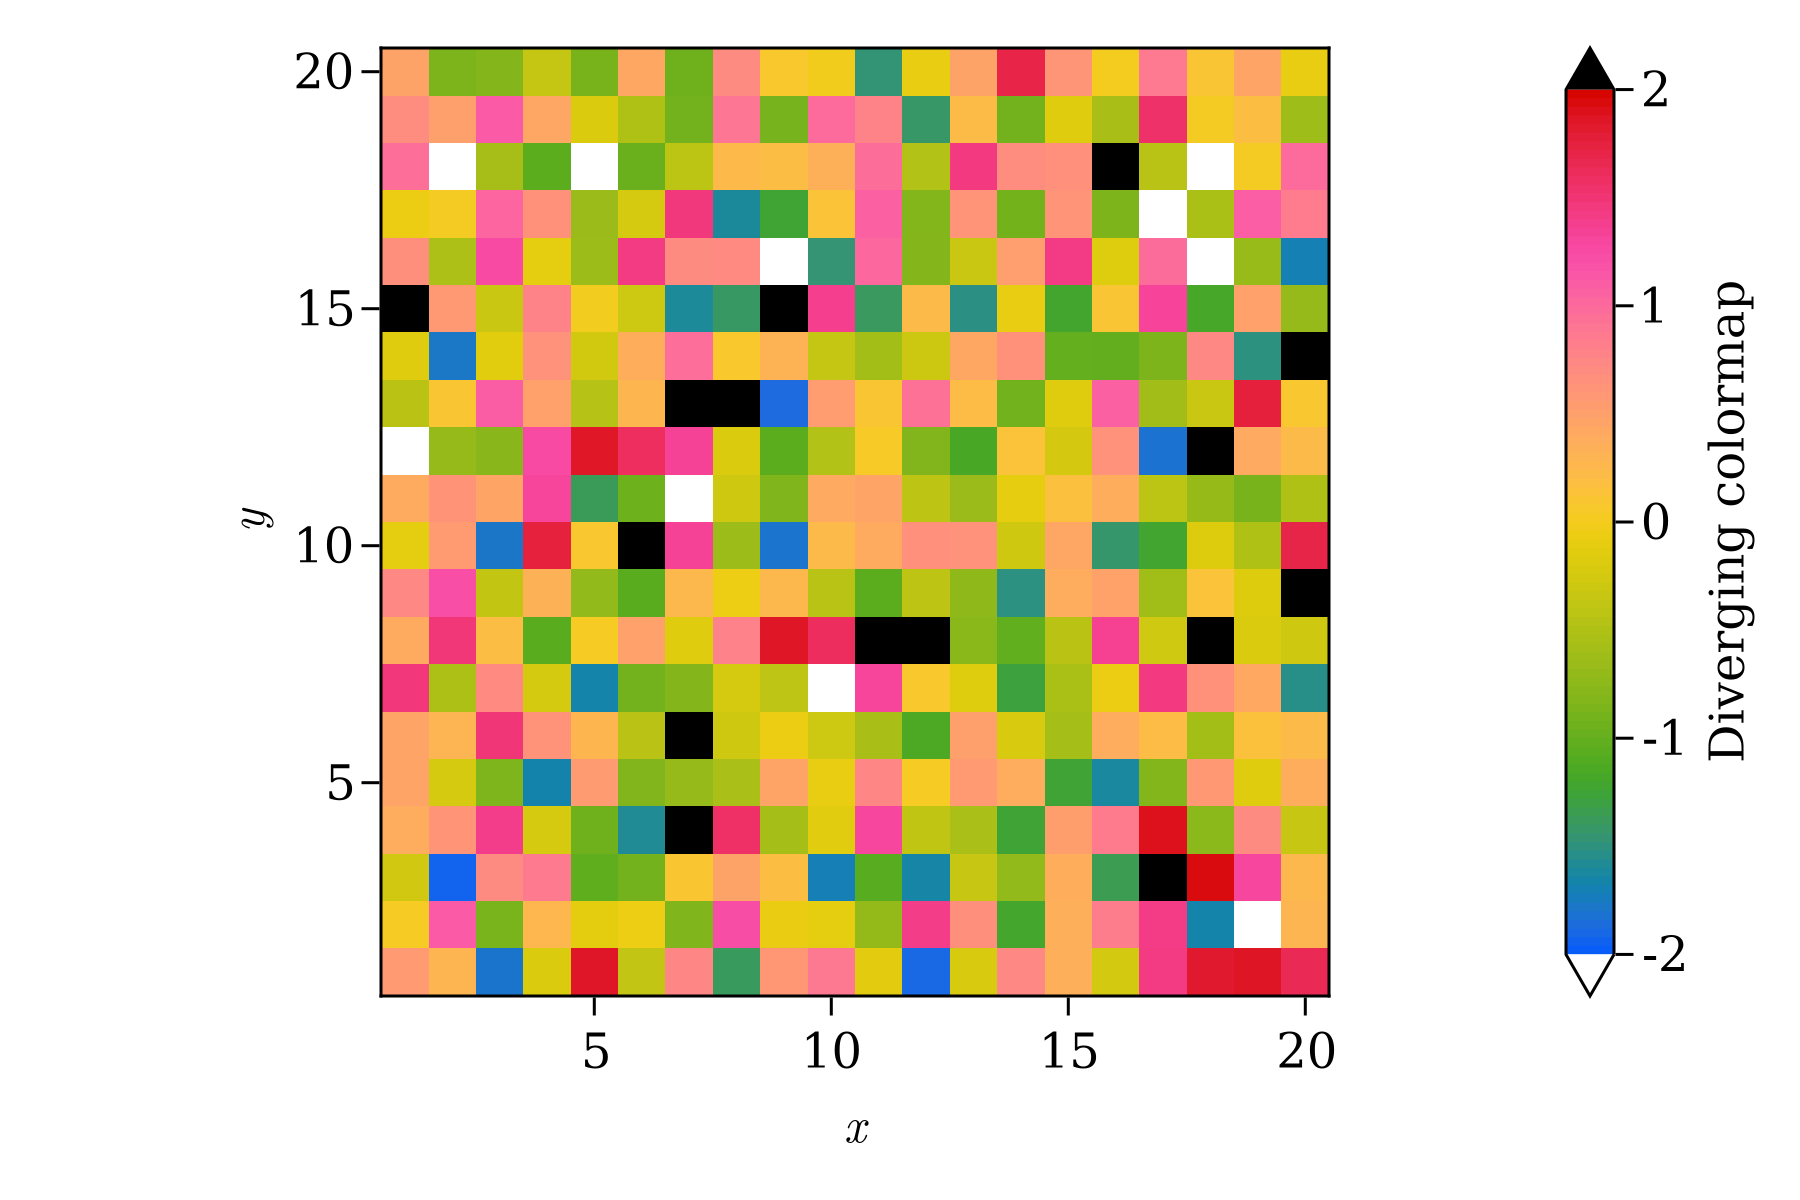
\includegraphics[width=0.6\textwidth,height=\textheight]{_build/im/diverging_colormap.png}
\caption{Diverging Colormap with low and high
clip.}\label{fig:diverging_colormap}
}
\end{figure}

另外 \passthrough{\lstinline!RGB!} 向量也是合法的选项。 在下面的例子中,
你可以传递一个自定义颜色图 \emph{perse} 或使用
\passthrough{\lstinline!cgrad!} 来创建分类值的
\passthrough{\lstinline!Colorbar!}。

\begin{lstlisting}
using Colors, ColorSchemes
\end{lstlisting}

\begin{lstlisting}[language=Julia]
figure = (; resolution=(600, 400), font="CMU Serif")
axis = (; xlabel=L"x", ylabel=L"y", aspect=DataAspect())
cmap = ColorScheme(range(colorant"red", colorant"green", length=3))
mygrays = ColorScheme([RGB{Float64}(i, i, i) for i in [0.0, 0.5, 1.0]])
fig, ax, pltobj = heatmap(rand(-1:1, 20, 20);
    colormap=cgrad(mygrays, 3, categorical=true, rev=true), # cgrad and Symbol, mygrays,
    axis=axis, figure=figure)
cbar = Colorbar(fig[1, 2], pltobj, label="Categories")
cbar.ticks = ([-0.66, 0, 0.66], ["-1", "0", "1"])
fig
\end{lstlisting}

\begin{figure}
\hypertarget{fig:categorical_colormap}{%
\centering
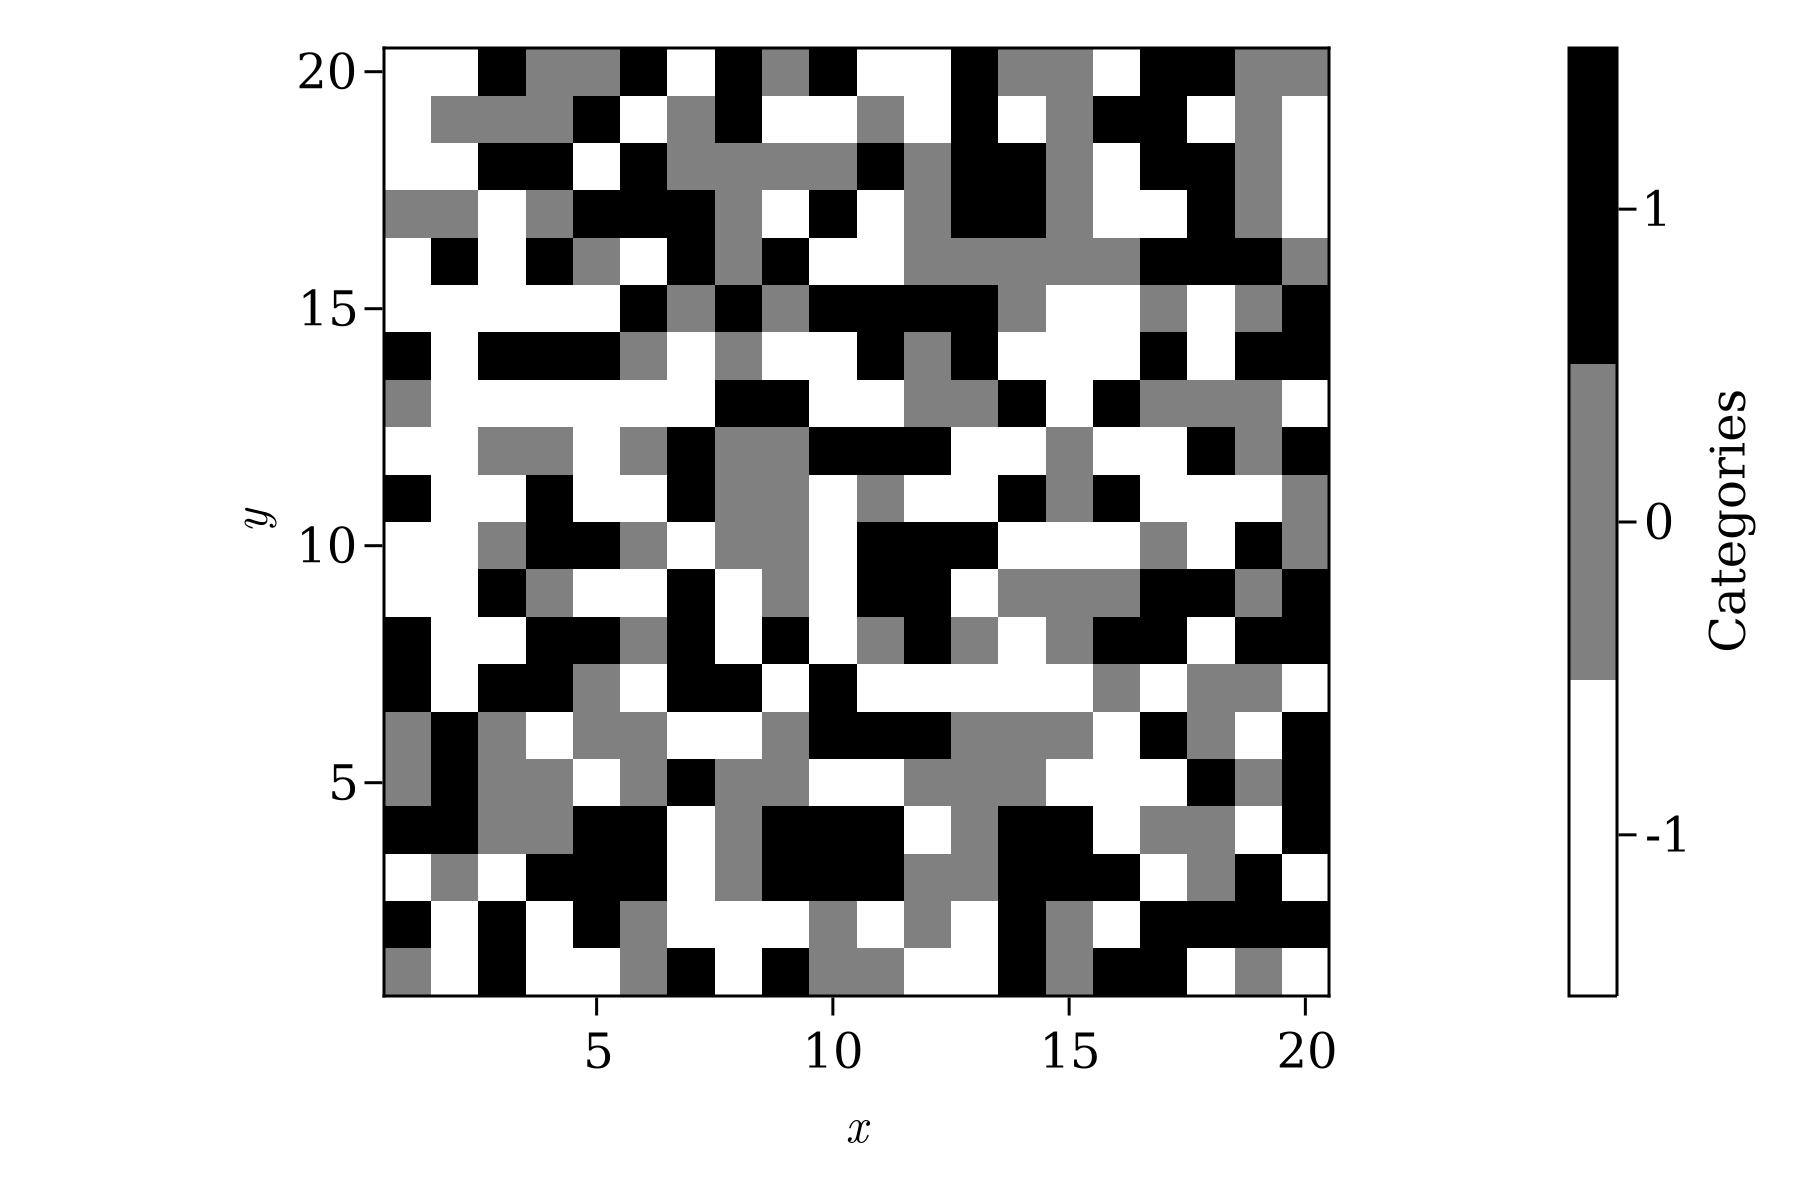
\includegraphics[width=0.6\textwidth,height=\textheight]{_build/im/categorical_colormap.png}
\caption{Categorical Colormap.}\label{fig:categorical_colormap}
}
\end{figure}

最后,分类值的颜色栏标签默认不在每种颜色间居中。
添加自定义标签可修复此问题,即
\passthrough{\lstinline!cbar.ticks = (positions, ticks)!}。
最后一种情况是传递颜色的元组给
\passthrough{\lstinline!colormap!},其中颜色可以通过
\passthrough{\lstinline!Symbol!}, \passthrough{\lstinline!String!}
或它们的混合指定。 然后将会得到这两组颜色间的插值颜色图。

另外,也支持十六进制编码的颜色作为输入。因此作为示范,下例将在热力图上放置一个半透明的标记。

\begin{lstlisting}[language=Julia]
figure = (; resolution=(600, 400), font="CMU Serif")
axis = (; xlabel=L"x", ylabel=L"y", aspect=DataAspect())
fig, ax, pltobj = heatmap(rand(20, 20); colorrange=(0, 1),
    colormap=(:red, "black"), axis=axis, figure=figure)
scatter!(ax, [11], [11], color=("#C0C0C0", 0.5), markersize=150)
Colorbar(fig[1, 2], pltobj, label="2 colors")
fig
\end{lstlisting}

\begin{figure}
\hypertarget{fig:colormap_two_colors}{%
\centering
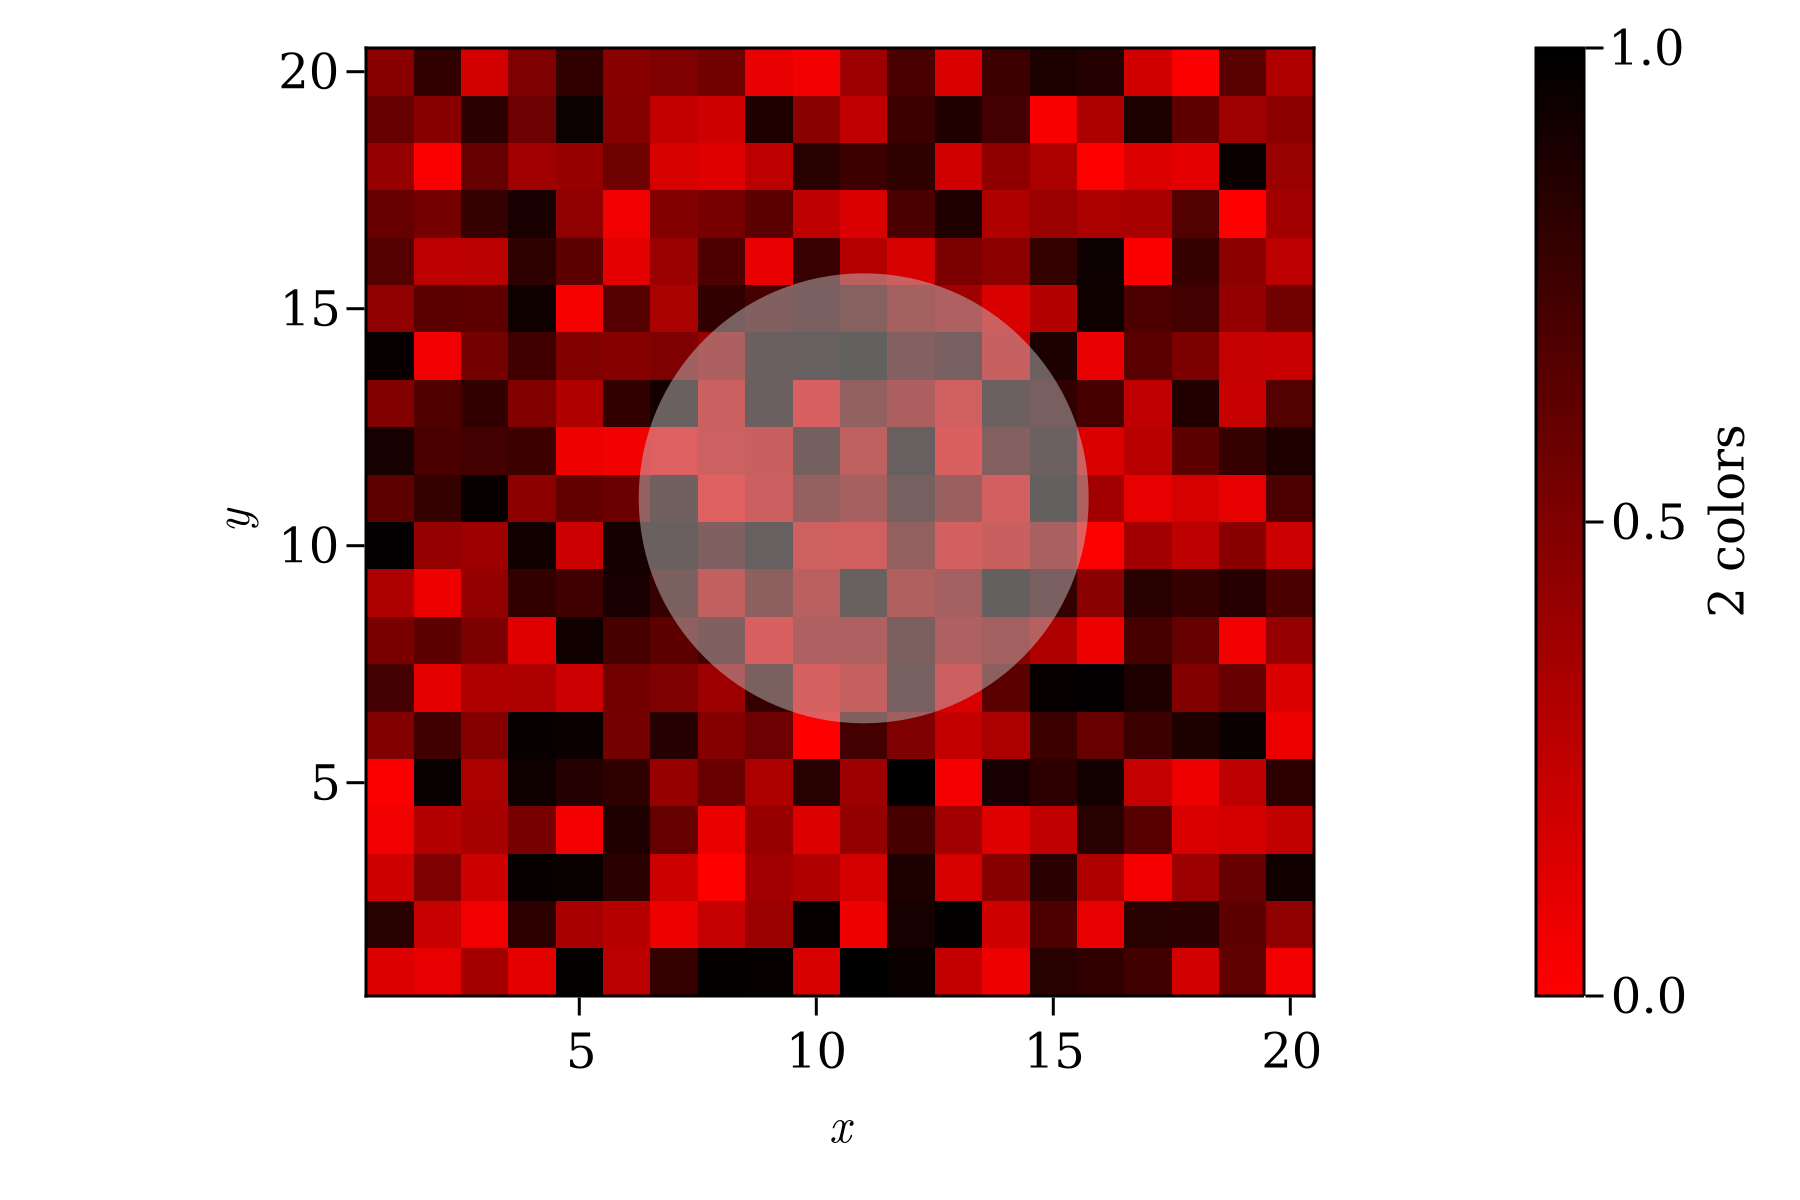
\includegraphics[width=0.6\textwidth,height=\textheight]{_build/im/colormap_two_colors.png}
\caption{Colormap from two colors.}\label{fig:colormap_two_colors}
}
\end{figure}

\hypertarget{ux81eaux5b9aux4e49ux989cux8272ux5faaux73af}{%
\subsection{自定义颜色循环}\label{ux81eaux5b9aux4e49ux989cux8272ux5faaux73af}}

可以通过新的颜色循环定义全局 \passthrough{\lstinline!Theme!} ,但通常
\textbf{不建议} 这样做。 更好的做法是定义新的主题并像上节那样使用它。
定义带有 \passthrough{\lstinline!:color!},
\passthrough{\lstinline!:linestyle!}, \passthrough{\lstinline!:marker!}
属性的新 \passthrough{\lstinline!cycle!} 和默认的
\passthrough{\lstinline!colormap!} 。 下面为之前的
\passthrough{\lstinline!publication\_theme!} 增加一些新的属性。

\begin{lstlisting}[language=Julia]
function new_cycle_theme()
    # https://nanx.me/ggsci/reference/pal_locuszoom.html
    my_colors = ["#D43F3AFF", "#EEA236FF", "#5CB85CFF", "#46B8DAFF",
        "#357EBDFF", "#9632B8FF", "#B8B8B8FF"]
    cycle = Cycle([:color, :linestyle, :marker], covary=true) # alltogether
    my_markers = [:circle, :rect, :utriangle, :dtriangle, :diamond,
        :pentagon, :cross, :xcross]
    my_linestyle = [nothing, :dash, :dot, :dashdot, :dashdotdot]
    Theme(
        fontsize=16, font="CMU Serif",
        colormap=:linear_bmy_10_95_c78_n256,
        palette=(color=my_colors, marker=my_markers, linestyle=my_linestyle),
        Lines=(cycle=cycle,), Scatter=(cycle=cycle,),
        Axis=(xlabelsize=20, xgridstyle=:dash, ygridstyle=:dash,
            xtickalign=1, ytickalign=1, yticksize=10, xticksize=10,
            xlabelpadding=-5, xlabel="x", ylabel="y"),
        Legend=(framecolor=(:black, 0.5), bgcolor=(:white, 0.5)),
        Colorbar=(ticksize=16, tickalign=1, spinewidth=0.5),
    )
end
\end{lstlisting}

然后将它应用到绘图函数中,如下所示:

\begin{lstlisting}[language=Julia]
function scatters_and_lines()
    x = collect(0:10)
    xh = LinRange(4, 6, 25)
    yh = LinRange(70, 95, 25)
    h = randn(25, 25)
    fig = Figure(resolution=(600, 400), font="CMU Serif")
    ax = Axis(fig[1, 1], xlabel=L"x", ylabel=L"f(x,a)")
    for i in x
        lines!(ax, x, i .* x; label=latexstring("$(i) x"))
        scatter!(ax, x, i .* x; markersize=13, strokewidth=0.25,
            label=latexstring("$(i) x"))
    end
    hm = heatmap!(xh, yh, h)
    axislegend(L"f(x)"; merge=true, position=:lt, nbanks=2, labelsize=14)
    Colorbar(fig[1, 2], hm, label="new default colormap")
    limits!(ax, -0.5, 10.5, -5, 105)
    colgap!(fig.layout, 5)
    fig
end
\end{lstlisting}

\begin{lstlisting}[language=Julia]
with_theme(scatters_and_lines, new_cycle_theme())
\end{lstlisting}

\begin{figure}
\hypertarget{fig:custom_cycle}{%
\centering
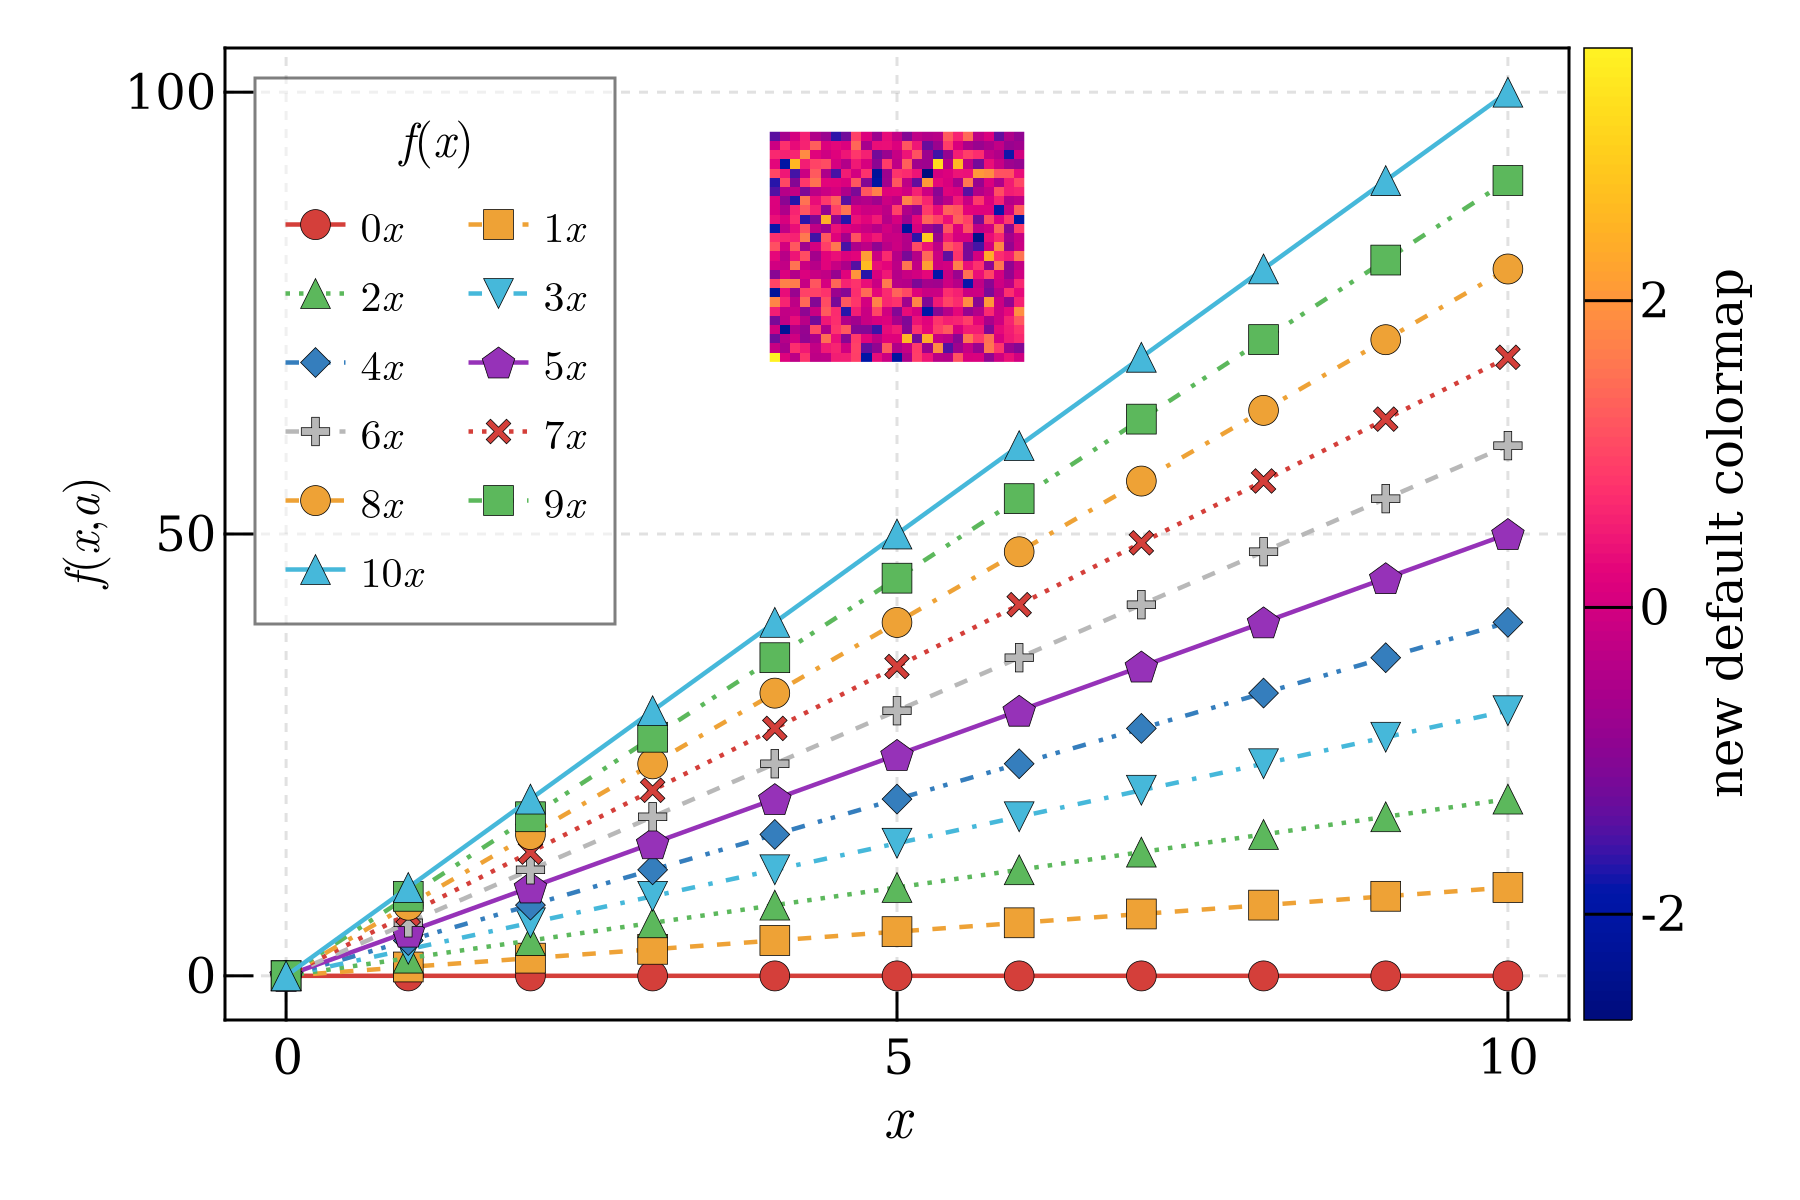
\includegraphics[width=0.6\textwidth,height=\textheight]{_build/im/custom_cycle.png}
\caption{Custom theme with new cycle and
colormap.}\label{fig:custom_cycle}
}
\end{figure}

此时,通过颜色,曲线样式,标记和颜色图,你已经能够 \textbf{完全控制}
绘图结果。 下一部分将讨论如何管理和控制 \textbf{布局}。

\hypertarget{sec:makie_layouts}{%
\section{布局}\label{sec:makie_layouts}}

一个完整的 \textbf{画布/布局} 是由 \passthrough{\lstinline!Figure!}
定义的,创建后将在其中填充各种内容。 下面将以一个包含
\passthrough{\lstinline!Axis!},\passthrough{\lstinline!Legend!} 和
\passthrough{\lstinline!Colorbar!} 的简单例子开始。 在这项任务中, 就像
\passthrough{\lstinline!Array!}/\passthrough{\lstinline!Matrix!}
那样,可以使用 \passthrough{\lstinline!rows!} 和
\passthrough{\lstinline!columns!} 索引
\passthrough{\lstinline!Figure!}。 \passthrough{\lstinline!Axis!} 位于
\textbf{第 1 行,第 1 列}, 即为 \passthrough{\lstinline!fig[1, 1]!}。
\passthrough{\lstinline!Colorbar!} 位于 \textbf{第 1 行,第 2 列}, 即为
\passthrough{\lstinline!fig[1, 2]!}。 另外,
\passthrough{\lstinline!Legend!} 位于 \textbf{第 2 行} 和 \textbf{第 1 -
2 列}, 即为 \passthrough{\lstinline!fig[2, 1:2]!}。

\begin{lstlisting}[language=Julia]
function first_layout()
    seed!(123)
    x, y, z = randn(6), randn(6), randn(6)
    fig = Figure(resolution=(600, 400), backgroundcolor=:grey90)
    ax = Axis(fig[1, 1], backgroundcolor=:white)
    pltobj = scatter!(ax, x, y; color=z, label="scatters")
    lines!(ax, x, 1.1y; label="line")
    Legend(fig[2, 1:2], ax, "labels", orientation=:horizontal)
    Colorbar(fig[1, 2], pltobj, label="colorbar")
    fig
end
first_layout()
\end{lstlisting}

\begin{figure}
\hypertarget{fig:first_layout}{%
\centering
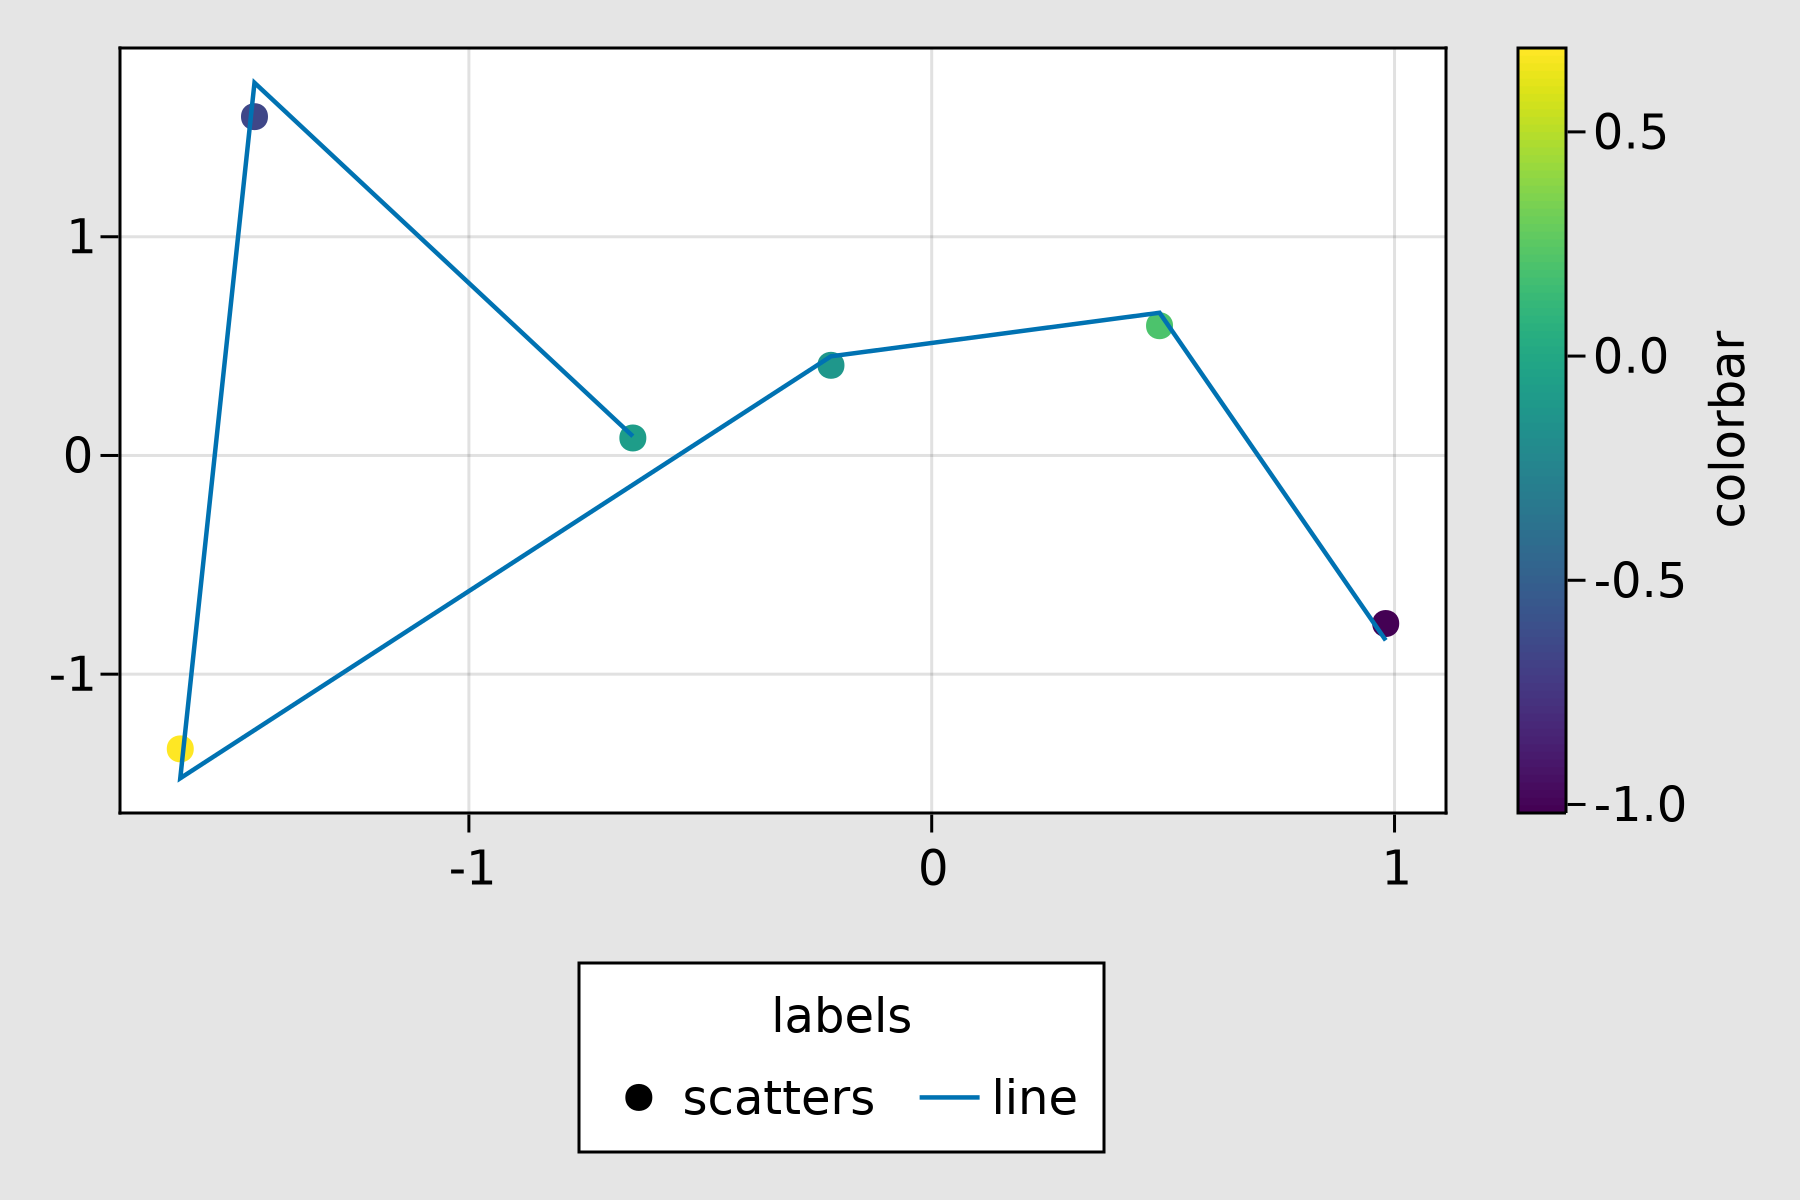
\includegraphics[width=0.6\textwidth,height=\textheight]{_build/im/JDS_first_layout_.png}
\caption{First Layout.}\label{fig:first_layout}
}
\end{figure}

这看起来已经不错了,但能变得更好。可以使用以下关键字和方法来解决图的间距问题:

\begin{itemize}
\tightlist
\item
  \passthrough{\lstinline!figure\_padding=(left, right, bottom, top)!}
\item
  \passthrough{\lstinline!padding=(left, right, bottom, top)!}
\end{itemize}

改变 \passthrough{\lstinline!Legend!} 或
\passthrough{\lstinline!Colorbar!} 实际大小的方法为:

\begin{quote}
\begin{itemize}
\tightlist
\item
  \passthrough{\lstinline!tellheight=true!} or
  \passthrough{\lstinline!false!}
\item
  \passthrough{\lstinline!tellwidth=true!} or
  \passthrough{\lstinline!false!}
\end{itemize}

\textbf{将这些设置为 \passthrough{\lstinline!true!} 后则需考虑
\passthrough{\lstinline!Legend!} 或 \passthrough{\lstinline!Colorbar!}
的实际大小(高或宽)。} 然后这些内容将会相应地调整大小。
\end{quote}

可以使用以下方法指定行和列的间距:

\begin{quote}
\begin{itemize}
\tightlist
\item
  \passthrough{\lstinline"colgap!(fig.layout, col, separation)"}
\item
  \passthrough{\lstinline"rowgap!(fig.layout, row, separation)"}
\end{itemize}

\textbf{列间距} (\passthrough{\lstinline"colgap!"}),如果给定了
\passthrough{\lstinline!col!},那么间距将只应用在指定的列。
\textbf{行间距} (\passthrough{\lstinline"rowgap!"}),如果给定了
\passthrough{\lstinline!row!},那么间距将只应用在指定的行。
\end{quote}

接下来将学习如何将内容放进 \textbf{突出部分(protrusion)},即为
\textbf{标题 \passthrough{\lstinline!x!} 和
\passthrough{\lstinline!y!},或 \passthrough{\lstinline!ticks!} 以及
\passthrough{\lstinline!label!}} 保留的空间。 实现方法是将位置索引改为
\passthrough{\lstinline!fig[i, j, protrusion]!}, 其中
\emph{\passthrough{\lstinline!protrusion!}} 可以是
\passthrough{\lstinline!Left()!},
\passthrough{\lstinline!Right()!},\passthrough{\lstinline!Bottom()!} 和
\passthrough{\lstinline!Top()!},或者是四个角
\passthrough{\lstinline!TopLeft()!},
\passthrough{\lstinline!TopRight()!},
\passthrough{\lstinline!BottomRight()!},\passthrough{\lstinline!BottomLeft()!}。
这些选项将在如下的例子中使用:

\begin{lstlisting}[language=Julia]
function first_layout_fixed()
    seed!(123)
    x, y, z = randn(6), randn(6), randn(6)
    fig = Figure(figure_padding=(0, 3, 5, 2), resolution=(600, 400),
        backgroundcolor=:grey90, font="CMU Serif")
    ax = Axis(fig[1, 1], xlabel=L"x", ylabel=L"y",
        title="Layout example", backgroundcolor=:white)
    pltobj = scatter!(ax, x, y; color=z, label="scatters")
    lines!(ax, x, 1.1y, label="line")
    Legend(fig[2, 1:2], ax, "Labels", orientation=:horizontal,
        tellheight=true, titleposition=:left)
    Colorbar(fig[1, 2], pltobj, label="colorbar")
    # additional aesthetics
    Box(fig[1, 1, Right()], color=(:slateblue1, 0.35))
    Label(fig[1, 1, Right()], "protrusion", textsize=18,
        rotation=pi / 2, padding=(3, 3, 3, 3))
    Label(fig[1, 1, TopLeft()], "(a)", textsize=18, padding=(0, 3, 8, 0))
    colgap!(fig.layout, 5)
    rowgap!(fig.layout, 5)
    fig
end
first_layout_fixed()
\end{lstlisting}

\begin{figure}
\hypertarget{fig:first_layout_fixed}{%
\centering
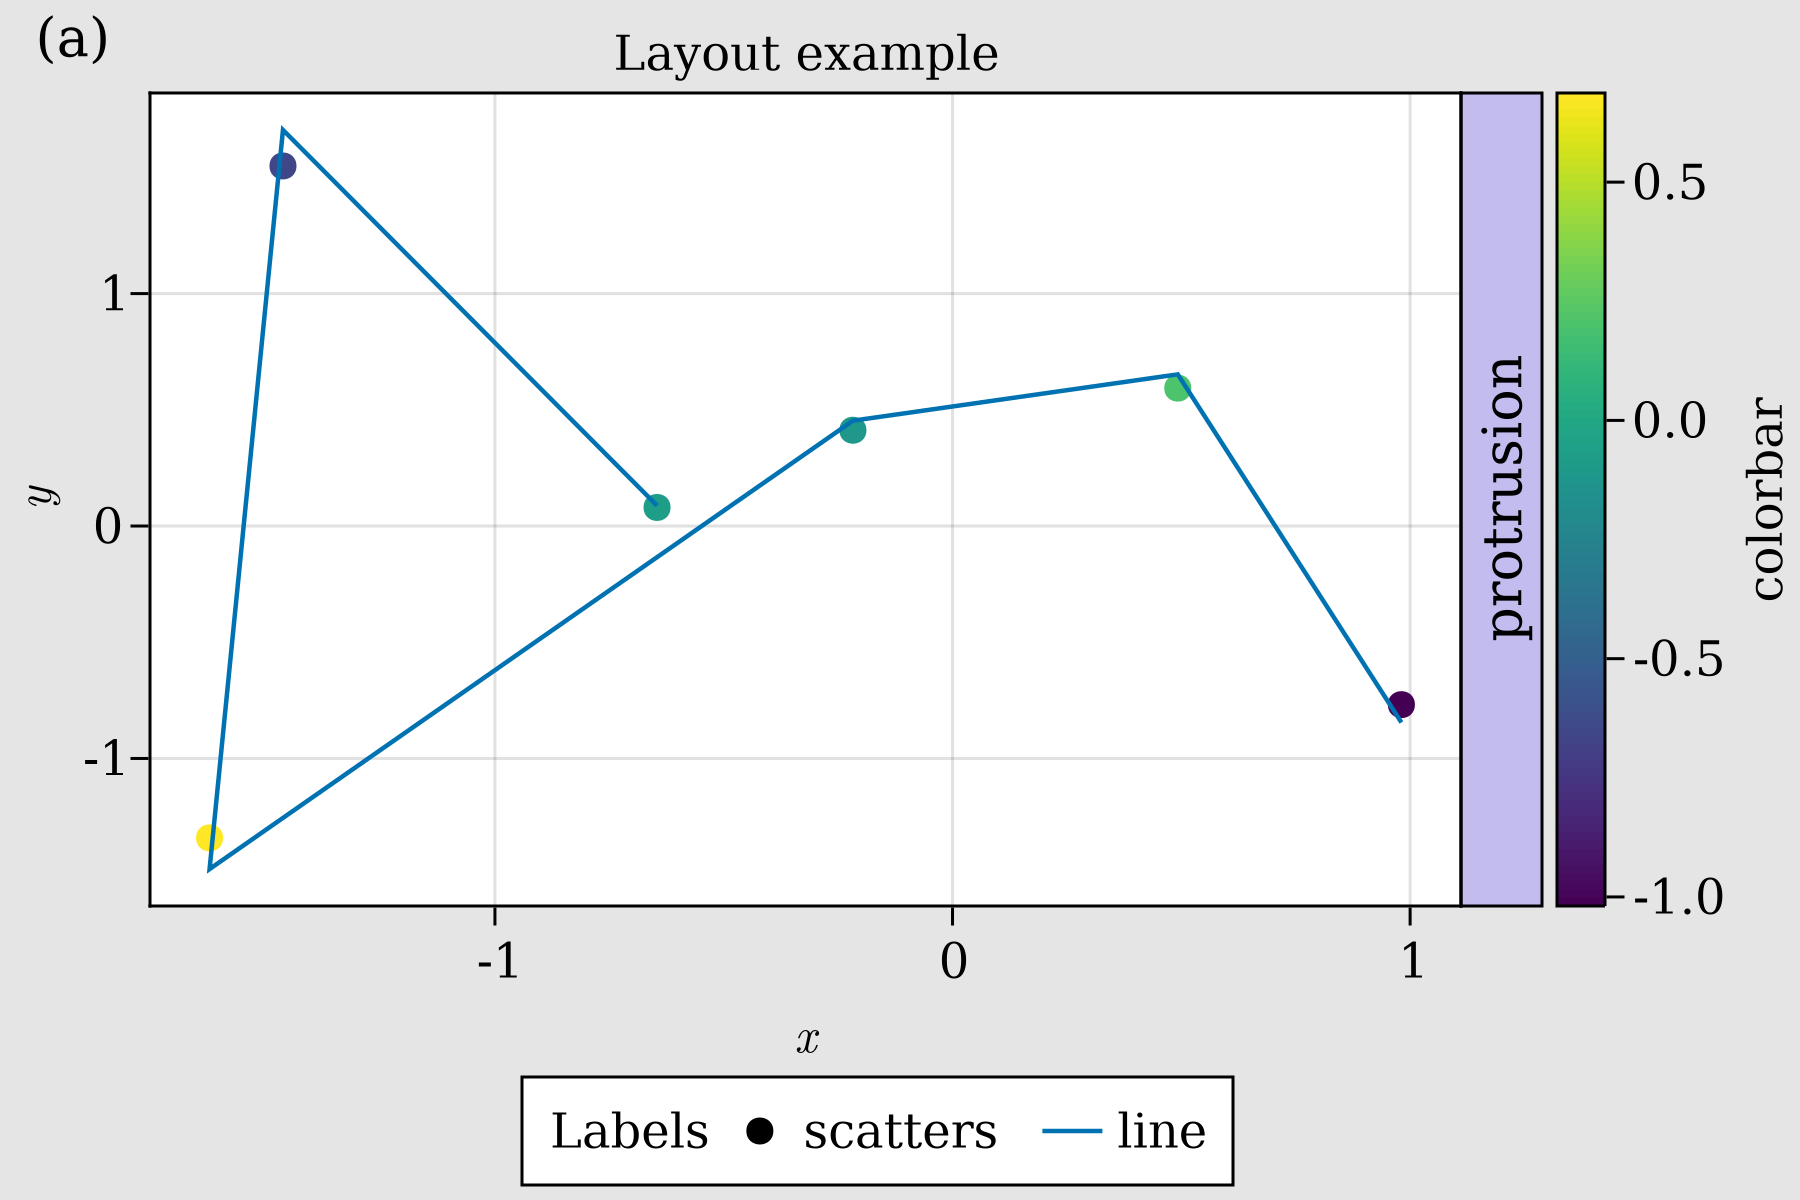
\includegraphics[width=0.6\textwidth,height=\textheight]{_build/im/JDS_first_layout_fixed_.png}
\caption{First Layout Fixed.}\label{fig:first_layout_fixed}
}
\end{figure}

这里在 \passthrough{\lstinline!TopLeft()!}添加标签
\passthrough{\lstinline!(a)!} 可能是不必要的,
因为标签仅在有两个以上的图时有意义。
在接下来的例子中,我们将继续使用之前的工具和一些新工具,并创建一个更丰富、更复杂的图。

可以使用以下函数隐藏图的装饰部分和轴线:

\begin{quote}
\begin{itemize}
\tightlist
\item
  \passthrough{\lstinline"hidedecorations!(ax; kwargs...)"}
\item
  \passthrough{\lstinline"hidexdecorations!(ax; kwargs...)"}
\item
  \passthrough{\lstinline"hideydecorations!(ax; kwargs...)"}
\item
  \passthrough{\lstinline"hidespines!(ax; kwargs...)"}
\end{itemize}
\end{quote}

应记住总是可以调用 \passthrough{\lstinline!help!}
查看能够传递的参数,例如:

\begin{lstlisting}[language=Julia]
help(hidespines!)
\end{lstlisting}

\begin{lstlisting}[language=Output]
  hidespines!(la::Axis, spines::Symbol... = (:l, :r, :b, :t)...)

  Hide all specified axis spines. Hides all spines by default, otherwise
  choose with the symbols :l, :r, :b and :t.

  hidespines! has the following function signatures:

    (Vector, Vector)
    (Vector, Vector, Vector)
    (Matrix)

  Available attributes for Combined{Makie.MakieLayout.hidespines!} are:

  
\end{lstlisting}

另外,对于 \passthrough{\lstinline"hidedecorations!"} 有:

\begin{lstlisting}[language=Julia]
help(hidedecorations!)
\end{lstlisting}

\begin{lstlisting}[language=Output]
  hidedecorations!(la::Axis)

  Hide decorations of both x and y-axis: label, ticklabels, ticks and grid.

  hidedecorations! has the following function signatures:

    (Vector, Vector)
    (Vector, Vector, Vector)
    (Matrix)

  Available attributes for Combined{Makie.MakieLayout.hidedecorations!} are:

  
\end{lstlisting}

对于 \textbf{不想隐藏的} 元素,仅需要将它们的值设置为
\passthrough{\lstinline!false!},即
\passthrough{\lstinline"hideydecorations!(ax; ticks=false, grid=false)"}。

同步 \passthrough{\lstinline!Axis!} 的方式如下:

\begin{quote}
\begin{itemize}
\tightlist
\item
  \passthrough{\lstinline"linkaxes!"},
  \passthrough{\lstinline"linkyaxes!"} 和
  \passthrough{\lstinline"linkxaxes!"}
\end{itemize}

这在需要共享轴时会变得很有用。 另一种获得共享轴的方法是设置
\passthrough{\lstinline"limits!"}。
\end{quote}

使用以下方式可一次性设定\passthrough{\lstinline!limits!},当然也能单独为每个方向的轴单独设定:

\begin{quote}
\begin{itemize}
\tightlist
\item
  \passthrough{\lstinline"limits!(ax; l, r, b, t)"},其中
  \passthrough{\lstinline!l!} 为左侧, \passthrough{\lstinline!r!}
  右侧,\passthrough{\lstinline!b!} 底部, 和
  \passthrough{\lstinline!t!} 顶部。
\end{itemize}

还能使用 \passthrough{\lstinline"ylims!(low, high)"} 或
\passthrough{\lstinline"xlims!(low, high)"},甚至可以通过
\passthrough{\lstinline"ylims!(low=0)"} 或
\passthrough{\lstinline"xlims!(high=1)"} 只设定一边。
\end{quote}

例子如下:

\begin{lstlisting}[language=Julia]
function complex_layout_double_axis()
    seed!(123)
    x = LinRange(0, 1, 10)
    y = LinRange(0, 1, 10)
    z = rand(10, 10)
    fig = Figure(resolution=(600, 400), font="CMU Serif", backgroundcolor=:grey90)
    ax1 = Axis(fig, xlabel=L"x", ylabel=L"y")
    ax2 = Axis(fig, xlabel=L"x")
    heatmap!(ax1, x, y, z; colorrange=(0, 1))
    series!(ax2, abs.(z[1:4, :]); labels=["lab $i" for i = 1:4], color=:Set1_4)
    hm = scatter!(10x, y; color=z[1, :], label="dots", colorrange=(0, 1))
    hideydecorations!(ax2, ticks=false, grid=false)
    linkyaxes!(ax1, ax2)
    #layout
    fig[1, 1] = ax1
    fig[1, 2] = ax2
    Label(fig[1, 1, TopLeft()], "(a)", textsize=18, padding=(0, 6, 8, 0))
    Label(fig[1, 2, TopLeft()], "(b)", textsize=18, padding=(0, 6, 8, 0))
    Colorbar(fig[2, 1:2], hm, label="colorbar", vertical=false, flipaxis=false)
    Legend(fig[1, 3], ax2, "Legend")
    colgap!(fig.layout, 5)
    rowgap!(fig.layout, 5)
    fig
end
complex_layout_double_axis()
\end{lstlisting}

\begin{figure}
\hypertarget{fig:complex_layout_double_axis}{%
\centering
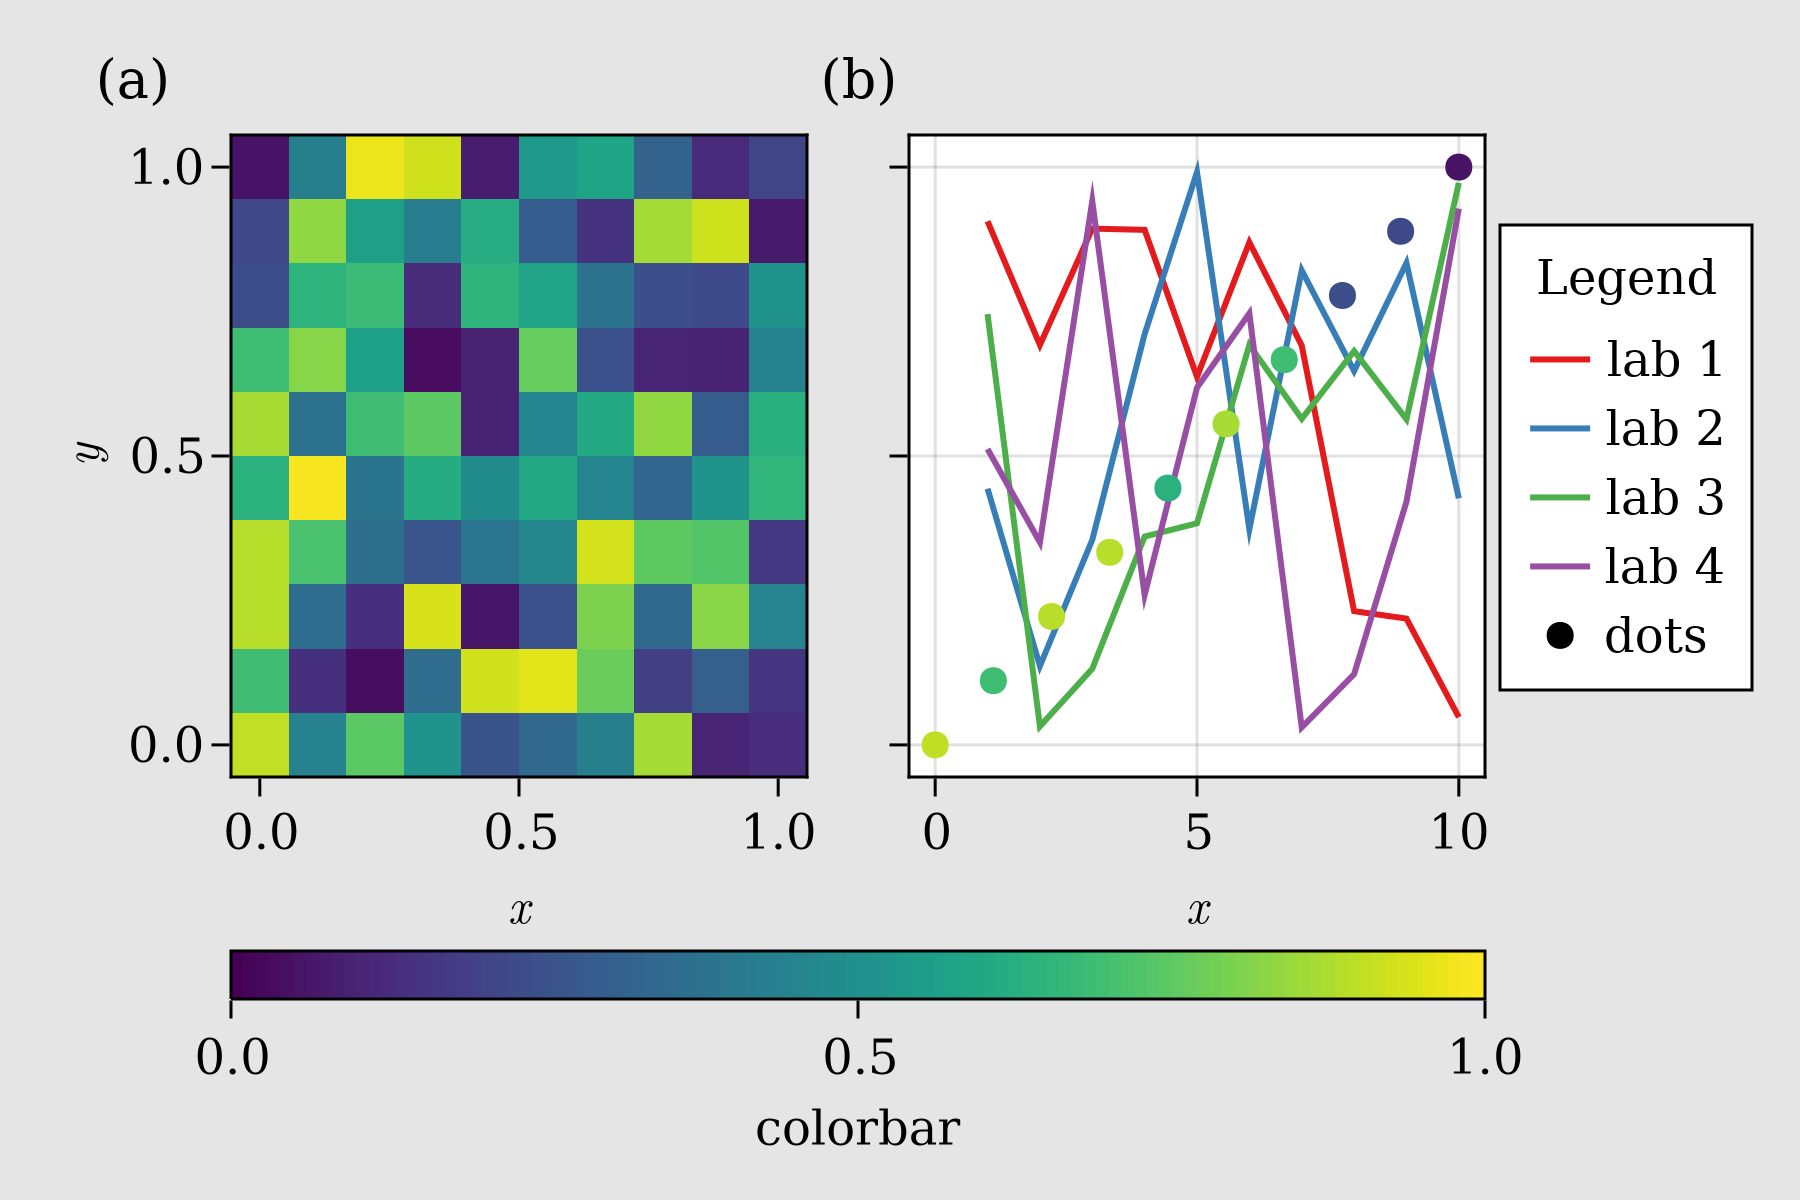
\includegraphics[width=0.6\textwidth,height=\textheight]{_build/im/JDS_complex_layout_double_axis_.png}
\caption{Complex layout double
axis.}\label{fig:complex_layout_double_axis}
}
\end{figure}

如上所示, \passthrough{\lstinline!Colorbar!}
的方向已经变为水平且它的标签也处在其下方。 这是因为设定了
\passthrough{\lstinline!vertical=false!} 和
\passthrough{\lstinline!flipaxis=false!}。 另外,也可以将更多的
\passthrough{\lstinline!Axis!} 添加到 \passthrough{\lstinline!fig!}
里,甚至可以是 \passthrough{\lstinline!Colorbar!} 和
\passthrough{\lstinline!Legend!},然后再构建布局。

另一种常见布局是热力图组成的正方网格:

\begin{lstlisting}[language=Julia]
function squares_layout()
    seed!(123)
    letters = reshape(collect('a':'d'), (2, 2))
    fig = Figure(resolution=(600, 400), fontsize=14, font="CMU Serif",
        backgroundcolor=:grey90)
    axs = [Axis(fig[i, j], aspect=DataAspect()) for i = 1:2, j = 1:2]
    hms = [heatmap!(axs[i, j], randn(10, 10), colorrange=(-2, 2))
           for i = 1:2, j = 1:2]
    Colorbar(fig[1:2, 3], hms[1], label="colorbar")
    [Label(fig[i, j, TopLeft()], "($(letters[i, j]))", textsize=16,
        padding=(-2, 0, -20, 0)) for i = 1:2, j = 1:2]
    colgap!(fig.layout, 5)
    rowgap!(fig.layout, 5)
    fig
end
squares_layout()
\end{lstlisting}

\begin{figure}
\hypertarget{fig:squares_layout}{%
\centering
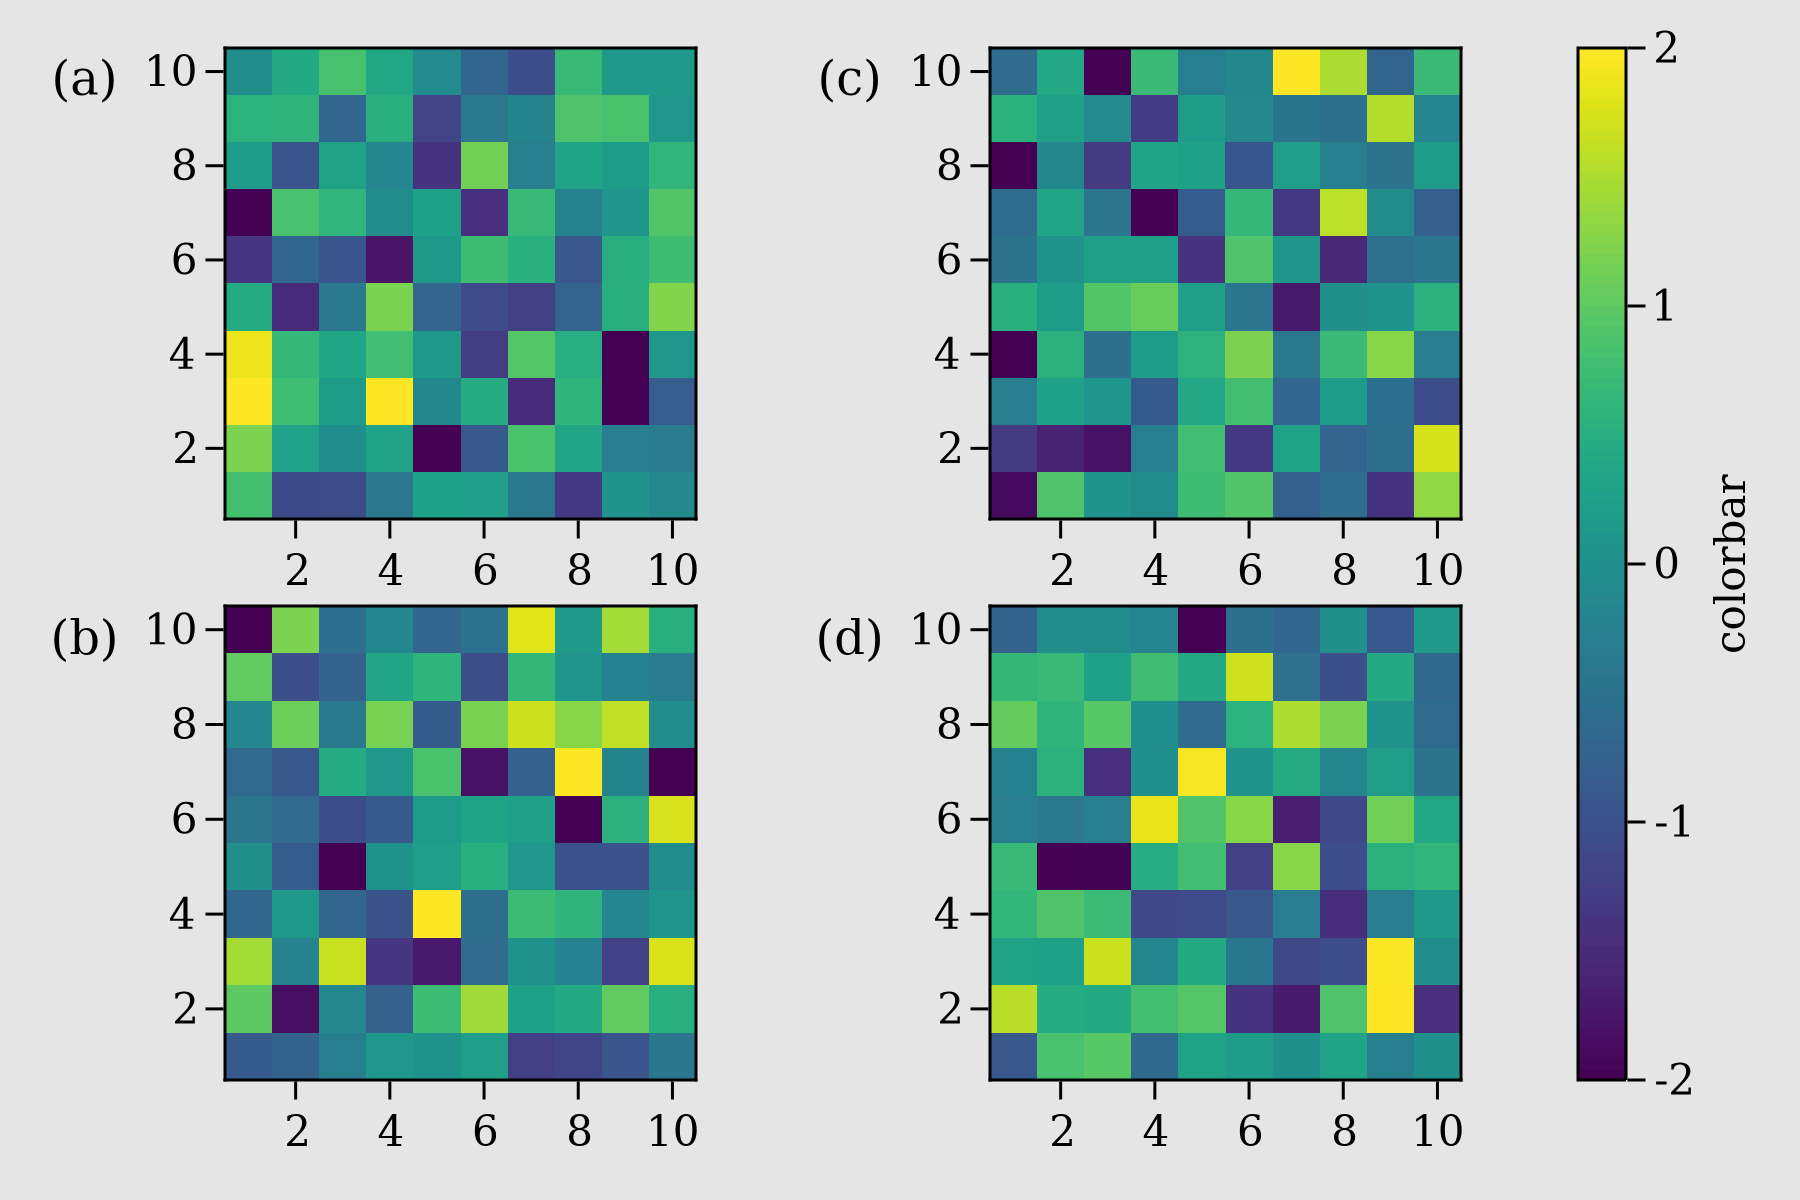
\includegraphics[width=0.6\textwidth,height=\textheight]{_build/im/JDS_squares_layout_.png}
\caption{Squares layout.}\label{fig:squares_layout}
}
\end{figure}

上图中每一个标签都位于 \textbf{突出部分} 并且每一个
\passthrough{\lstinline!Axis!} 都有
\passthrough{\lstinline!AspectData()!} 率属性。 图中
\passthrough{\lstinline!Colorbar!} 位于第三列,并从第一行跨到第二行。

下例将使用称为 \passthrough{\lstinline!Mixed()!}
的\textbf{对齐模式},这在处理 \passthrough{\lstinline!Axis!}
间的大量空白区域时很有用,而这些空白区域通常是由长标签导致的。
另外,本例还需要使用 Julia 标准库中的 \passthrough{\lstinline!Dates!} 。

\begin{lstlisting}
using Dates
\end{lstlisting}

\begin{lstlisting}[language=Julia]
function mixed_mode_layout()
    seed!(123)
    longlabels = ["$(today() - Day(1))", "$(today())", "$(today() + Day(1))"]
    fig = Figure(resolution=(600, 400), fontsize=12,
        backgroundcolor=:grey90, font="CMU Serif")
    ax1 = Axis(fig[1, 1])
    ax2 = Axis(fig[1, 2], xticklabelrotation=pi / 2, alignmode=Mixed(bottom=0),
        xticks=([1, 5, 10], longlabels))
    ax3 = Axis(fig[2, 1:2])
    ax4 = Axis(fig[3, 1:2])
    axs = [ax1, ax2, ax3, ax4]
    [lines!(ax, 1:10, rand(10)) for ax in axs]
    hidexdecorations!(ax3; ticks=false, grid=false)
    Box(fig[2:3, 1:2, Right()], color=(:slateblue1, 0.35))
    Label(fig[2:3, 1:2, Right()], "protrusion", rotation=pi / 2, textsize=14,
        padding=(3, 3, 3, 3))
    Label(fig[1, 1:2, Top()], "Mixed alignmode", textsize=16,
        padding=(0, 0, 15, 0))
    colsize!(fig.layout, 1, Auto(2))
    rowsize!(fig.layout, 2, Auto(0.5))
    rowsize!(fig.layout, 3, Auto(0.5))
    rowgap!(fig.layout, 1, 15)
    rowgap!(fig.layout, 2, 0)
    colgap!(fig.layout, 5)
    fig
end
mixed_mode_layout()
\end{lstlisting}

\begin{figure}
\hypertarget{fig:mixed_mode_layout}{%
\centering
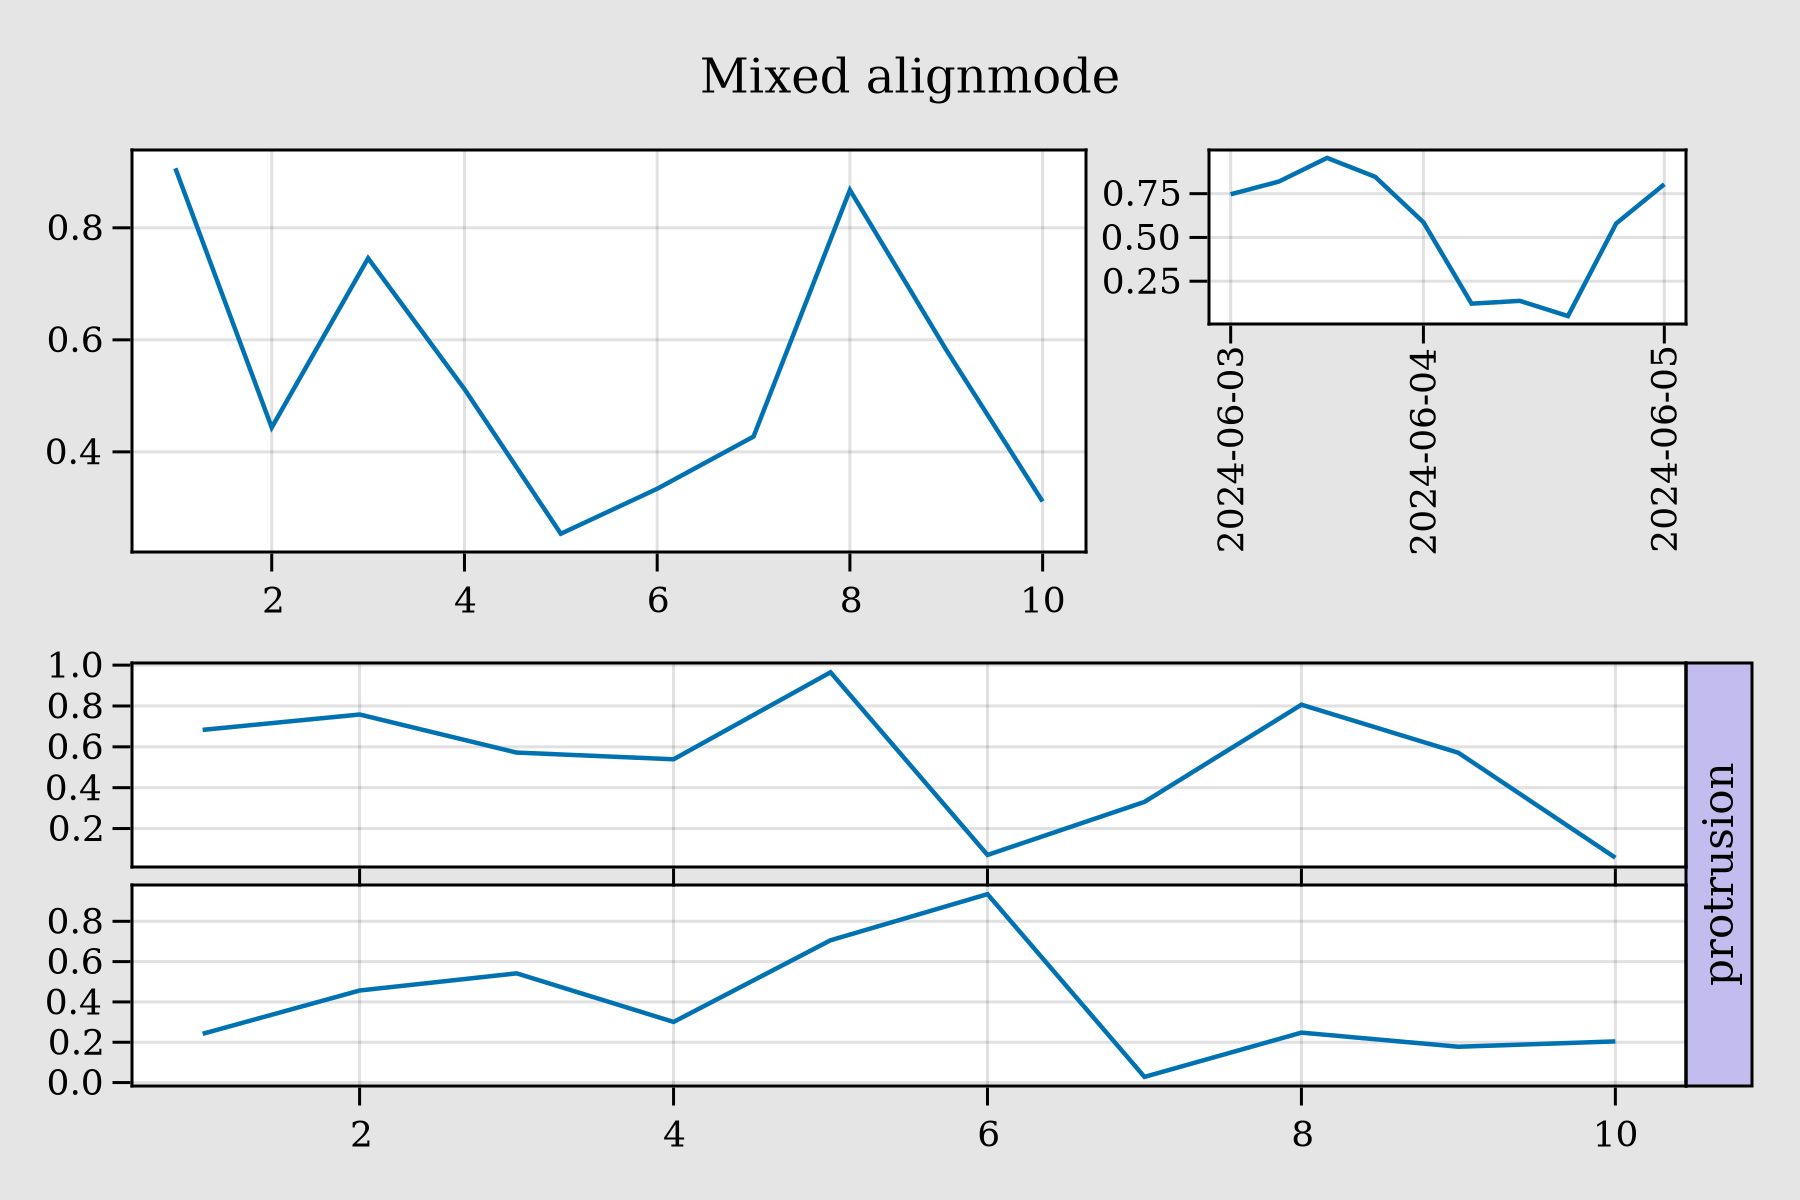
\includegraphics[width=0.6\textwidth,height=\textheight]{_build/im/JDS_mixed_mode_layout_.png}
\caption{Mixed mode layout.}\label{fig:mixed_mode_layout}
}
\end{figure}

如上,参数 \passthrough{\lstinline!alignmode=Mixed(bottom=0)!}
将边界框移动到底部,使其与左侧面板保持对齐。

从上图也可以看到 \passthrough{\lstinline"colsize!"} 和
\passthrough{\lstinline"rowsize!"} 如何作用于不同的行和列。
可以向函数传递一个数字而不是
\passthrough{\lstinline!Auto()!},但那会固定所有的设置。 另外, 在定义
\passthrough{\lstinline!Axis!} 时也可以设定
\passthrough{\lstinline!height!} 或
\passthrough{\lstinline!width!},例如
\passthrough{\lstinline!Axis(fig, heigth=50)!} 将会固定轴的高度。

\hypertarget{ux5d4cux5957-axis-subplots}{%
\subsection{\texorpdfstring{嵌套 \texttt{Axis}
(\emph{subplots})}{嵌套 Axis (subplots)}}\label{ux5d4cux5957-axis-subplots}}

精准定义一组 \passthrough{\lstinline!Axis!} (\emph{subplots})
也是可行的, 可以使用一组 \passthrough{\lstinline!Axis!}
构造具有多行多列的图。 例如,下面展示了一组较复杂的
\passthrough{\lstinline!Axis!}:

\begin{lstlisting}[language=Julia]
function nested_sub_plot!(fig)
    color = rand(RGBf)
    ax1 = Axis(fig[1, 1], backgroundcolor=(color, 0.25))
    ax2 = Axis(fig[1, 2], backgroundcolor=(color, 0.25))
    ax3 = Axis(fig[2, 1:2], backgroundcolor=(color, 0.25))
    ax4 = Axis(fig[1:2, 3], backgroundcolor=(color, 0.25))
    return (ax1, ax2, ax3, ax4)
end
\end{lstlisting}

当通过多次调用它来构建更复杂的图时,可以得到:

\begin{lstlisting}[language=Julia]
function main_figure()
    fig = Figure()
    Axis(fig[1, 1])
    nested_sub_plot!(fig[1, 2])
    nested_sub_plot!(fig[1, 3])
    nested_sub_plot!(fig[2, 1:3])
    fig
end
main_figure()
\end{lstlisting}

\begin{figure}
\hypertarget{fig:main_figure}{%
\centering
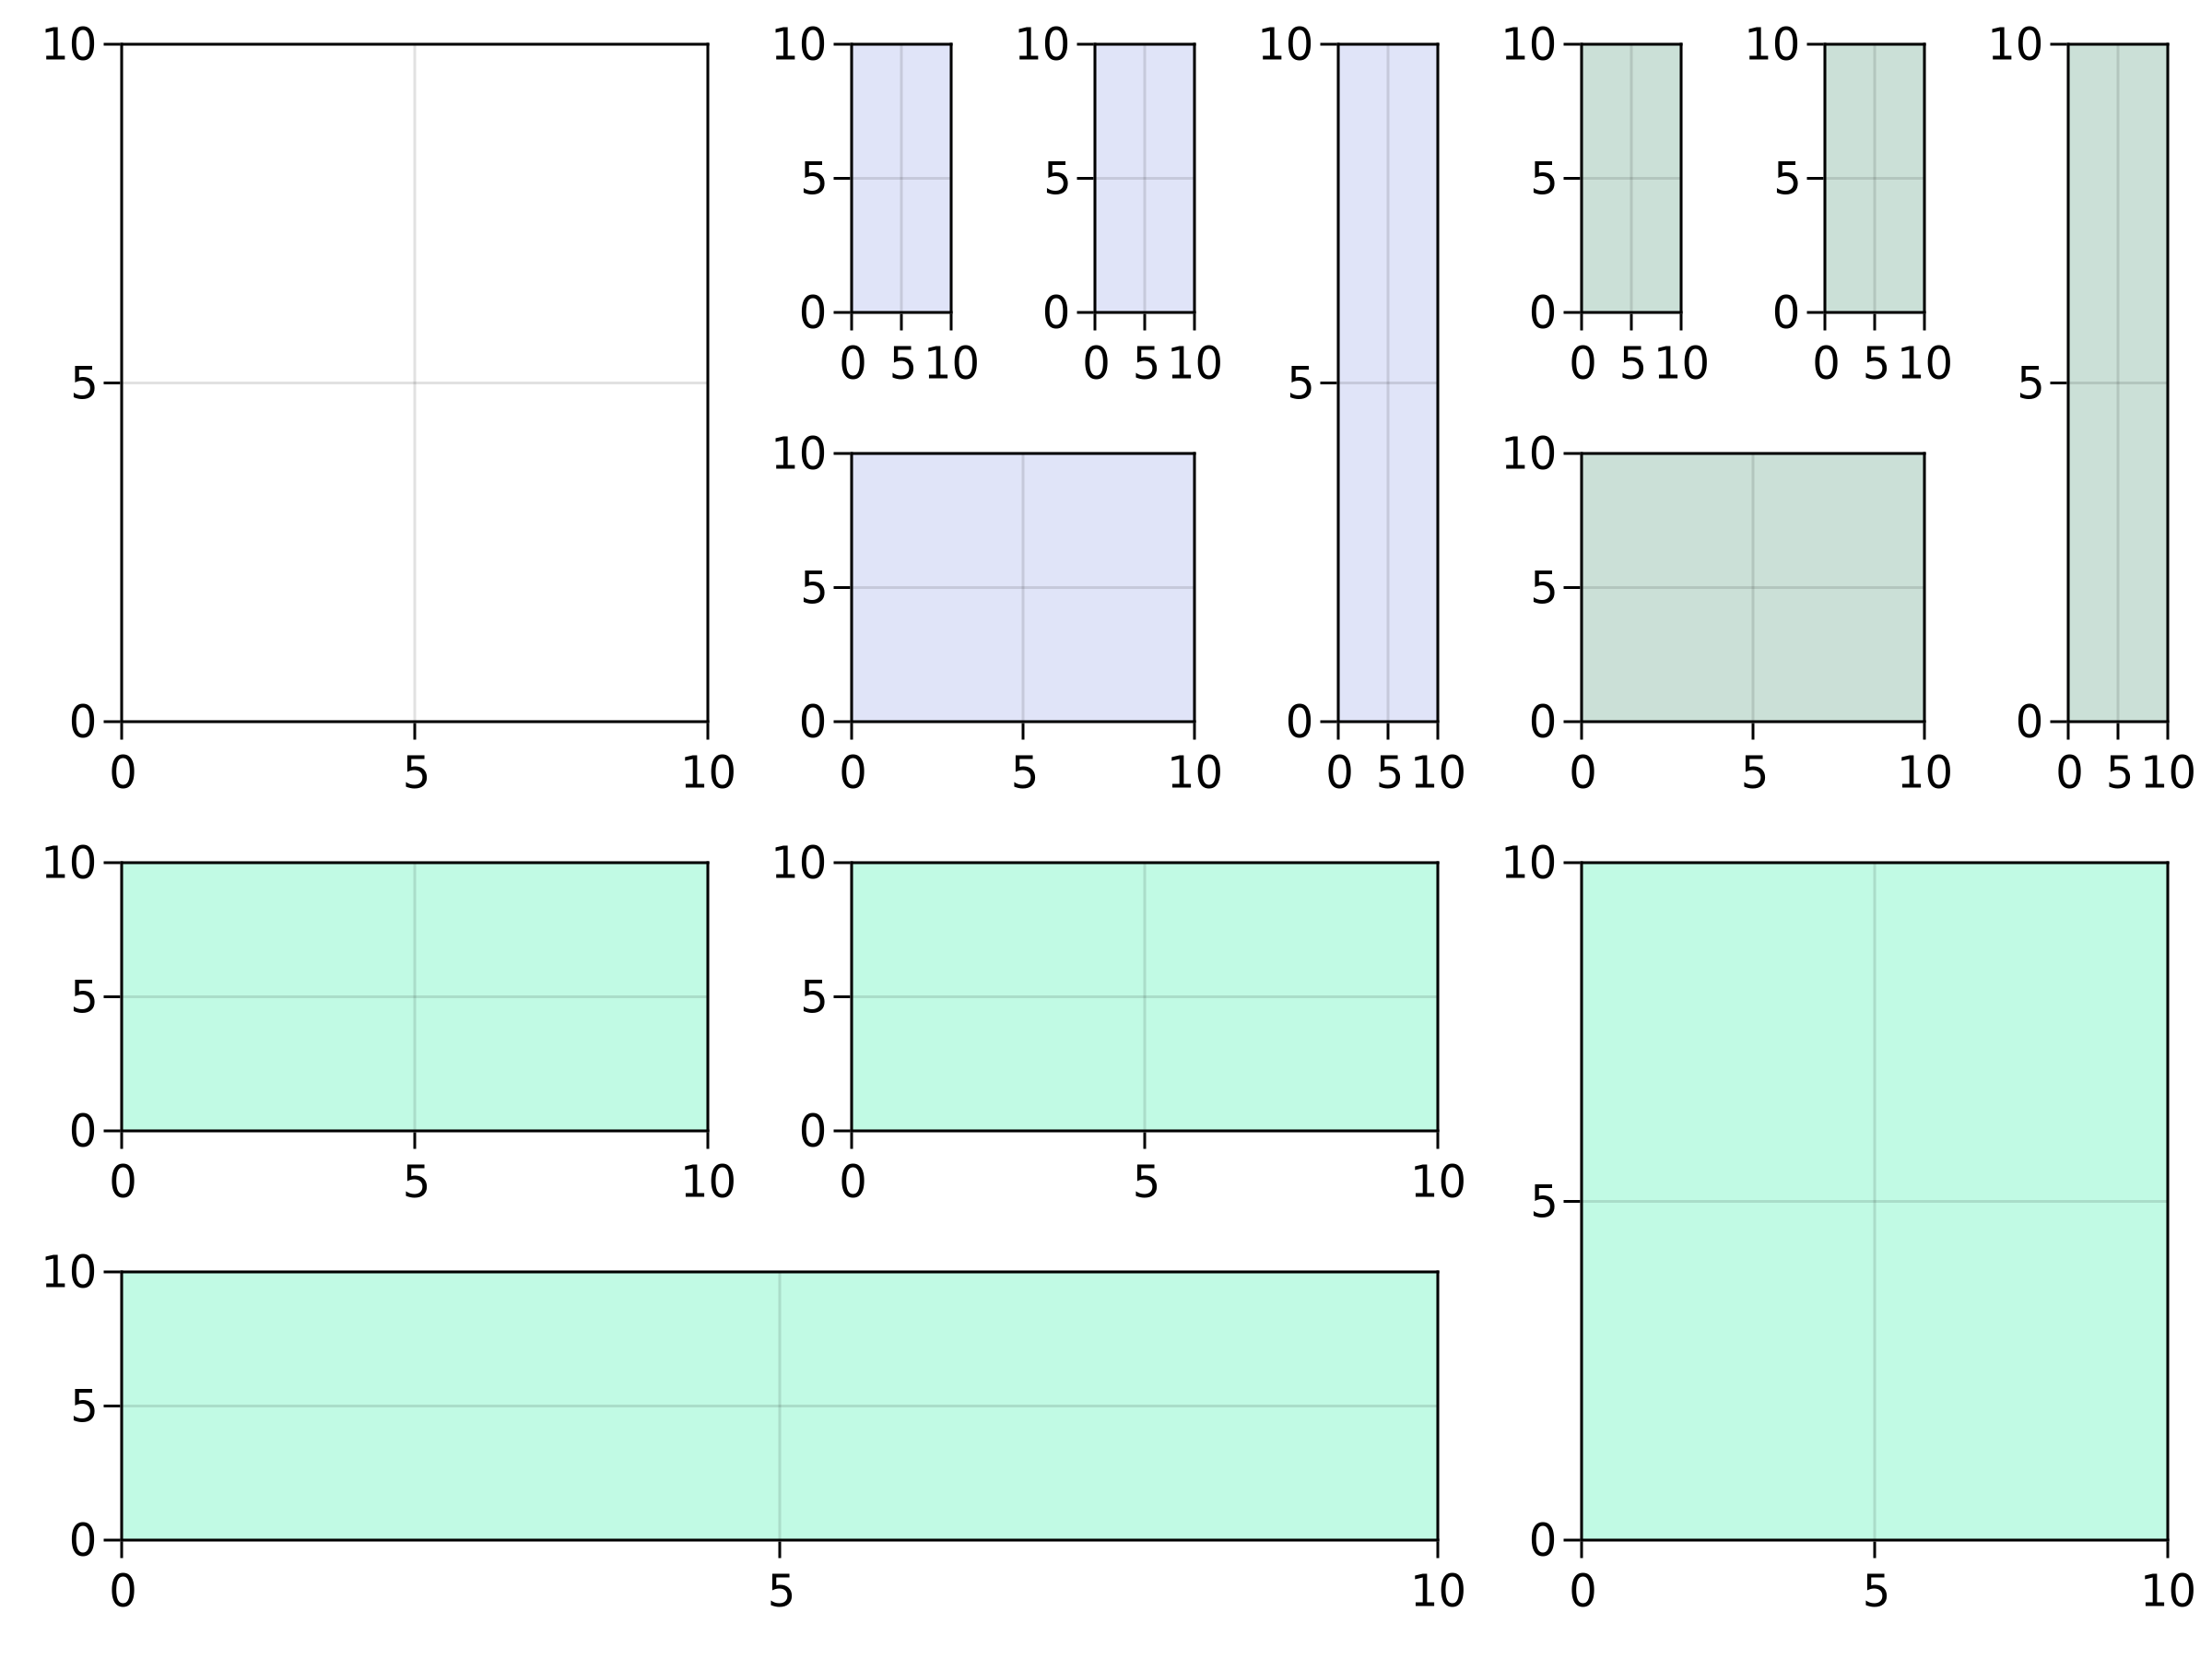
\includegraphics[width=0.6\textwidth,height=\textheight]{_build/im/JDS_main_figure_.png}
\caption{Main figure.}\label{fig:main_figure}
}
\end{figure}

注意,这里可以调用不同的子图函数。 另外,每一个
\passthrough{\lstinline!Axis!} 都是 \passthrough{\lstinline!Figure!}
的独立部分。 因此,当在进行 \passthrough{\lstinline"rowgap!"}或者
\passthrough{\lstinline"colsize!"}
这样的操作时,你需要考虑是对每一个子图单独作用还是对所有的图一起作用。

对于组合的 \passthrough{\lstinline!Axis!} (\emph{subplots}) 可以使用
\passthrough{\lstinline!GridLayout()!}, 它能用来构造更复杂的
\passthrough{\lstinline!Figure!}。

\hypertarget{ux5d4cux5957ux7f51ux683cux5e03ux5c40}{%
\subsection{嵌套网格布局}\label{ux5d4cux5957ux7f51ux683cux5e03ux5c40}}

可以使用 \passthrough{\lstinline!GridLayout()!}
组合子图,这种方法能够更自由地构建更复杂的图。 这里再次使用之前的
\passthrough{\lstinline"nested\_sub\_plot!"},它定义了三组子图和一个普通的
\passthrough{\lstinline!Axis!}:

\begin{lstlisting}[language=Julia]
function nested_Grid_Layouts()
    fig = Figure(backgroundcolor=RGBf(0.96, 0.96, 0.96))
    ga = fig[1, 1] = GridLayout()
    gb = fig[1, 2] = GridLayout()
    gc = fig[1, 3] = GridLayout()
    gd = fig[2, 1:3] = GridLayout()
    gA = Axis(ga[1, 1])
    nested_sub_plot!(gb)
    axsc = nested_sub_plot!(gc)
    nested_sub_plot!(gd)
    [hidedecorations!(axsc[i], grid=false, ticks=false) for i = 1:length(axsc)]
    colgap!(gc, 5)
    rowgap!(gc, 5)
    rowsize!(fig.layout, 2, Auto(0.5))
    colsize!(fig.layout, 1, Auto(0.5))
    fig
end
nested_Grid_Layouts()
\end{lstlisting}

\begin{figure}
\hypertarget{fig:nested_Grid_Layouts}{%
\centering
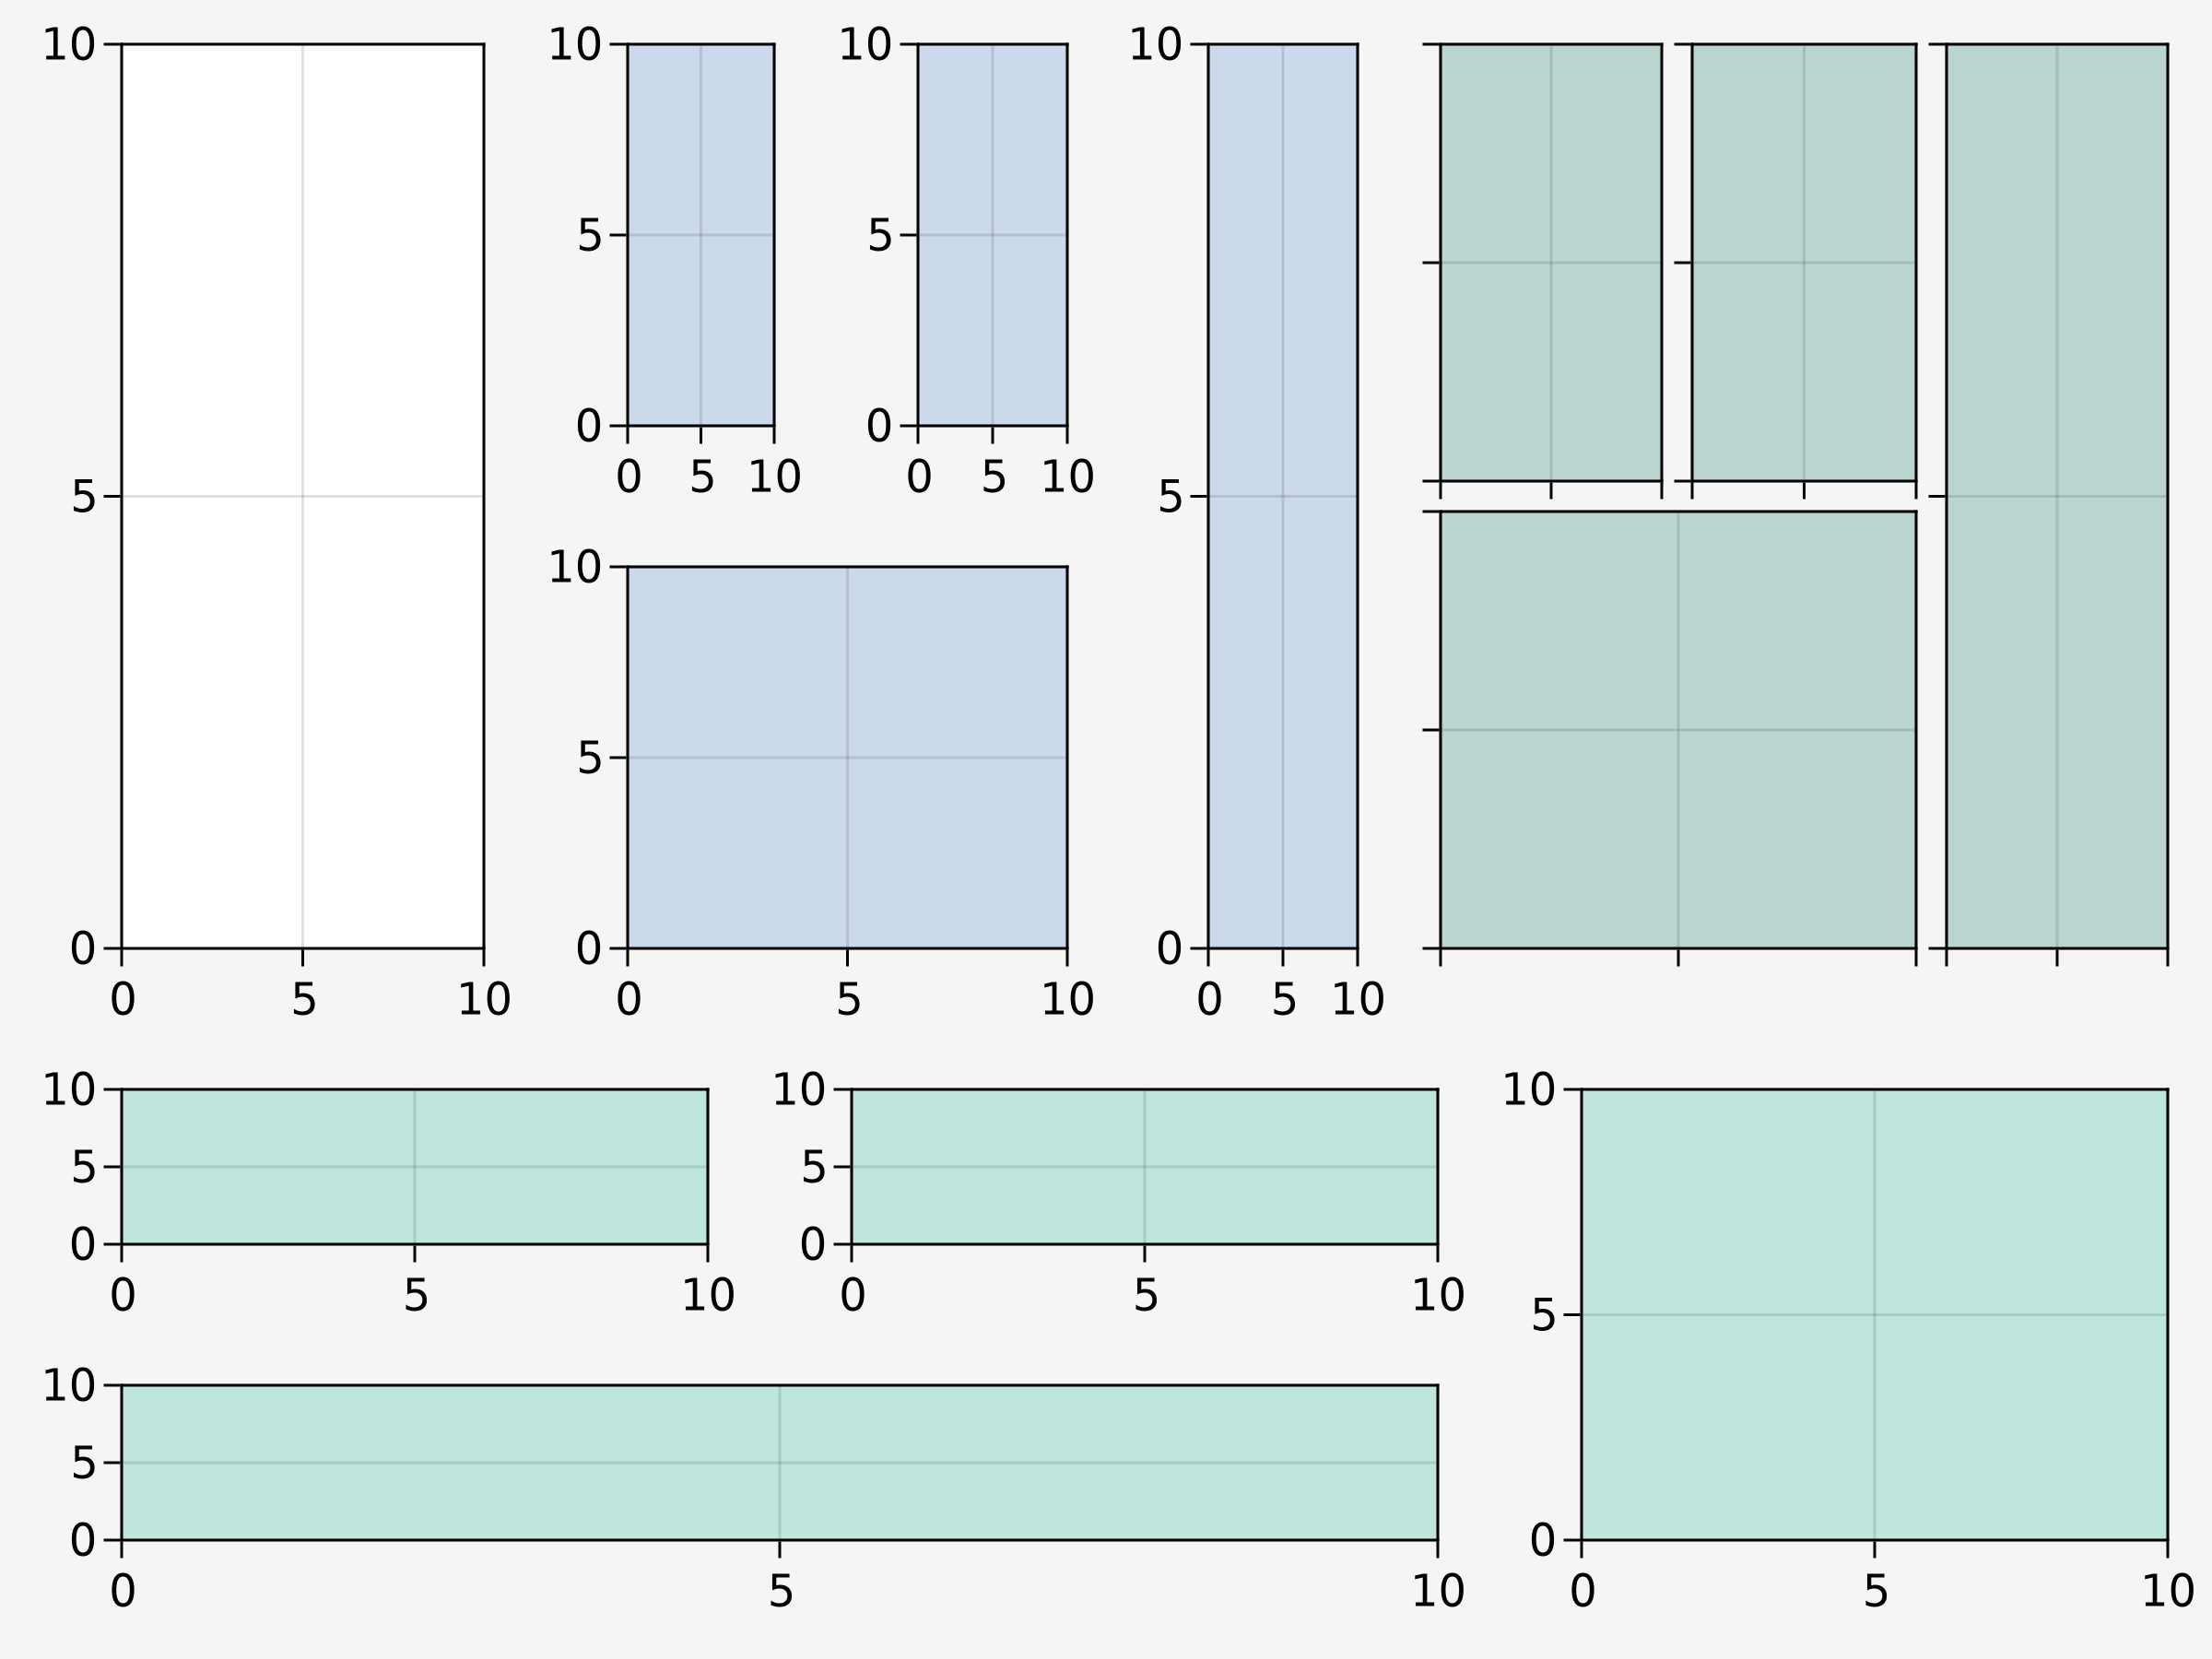
\includegraphics[width=0.6\textwidth,height=\textheight]{_build/im/JDS_nested_Grid_Layouts_.png}
\caption{Nested Grid Layouts.}\label{fig:nested_Grid_Layouts}
}
\end{figure}

现在,对每一组使用 \passthrough{\lstinline"rowgap!"} 或
\passthrough{\lstinline"colsize!"} 将是可行的,并且
\passthrough{\lstinline"rowsize!, colsize!"} 也能够应用于
\passthrough{\lstinline!GridLayout()!}。

\hypertarget{ux63d2ux56fe}{%
\subsection{插图}\label{ux63d2ux56fe}}

目前,绘制 \passthrough{\lstinline!inset!} 是一项棘手的工作。
本节展示两种在初始时通过定义辅助函数实现绘制插图的方法。 第一种是定义
\passthrough{\lstinline!BBox!},它存在于整个
\passthrough{\lstinline!Figure!} 空间:

\begin{lstlisting}[language=Julia]
function add_box_inset(fig; left=100, right=250, bottom=200, top=300,
    bgcolor=:grey90)
    inset_box = Axis(fig, bbox=BBox(left, right, bottom, top),
        xticklabelsize=12, yticklabelsize=12, backgroundcolor=bgcolor)
    # bring content upfront
    translate!(inset_box.scene, 0, 0, 10)
    elements = keys(inset_box.elements)
    filtered = filter(ele -> ele != :xaxis && ele != :yaxis, elements)
    foreach(ele -> translate!(inset_box.elements[ele], 0, 0, 9), filtered)
    return inset_box
end
\end{lstlisting}

然后可以按照如下方式轻松地绘制插图:

\begin{lstlisting}[language=Julia]
function figure_box_inset()
    fig = Figure(resolution=(600, 400))
    ax = Axis(fig[1, 1], backgroundcolor=:white)
    inset_ax1 = add_box_inset(fig; left=100, right=250, bottom=200, top=300,
        bgcolor=:grey90)
    inset_ax2 = add_box_inset(fig; left=500, right=600, bottom=100, top=200,
        bgcolor=(:white, 0.65))
    lines!(ax, 1:10)
    lines!(inset_ax1, 1:10)
    scatter!(inset_ax2, 1:10, color=:black)
    fig
end
figure_box_inset()
\end{lstlisting}

\begin{figure}
\hypertarget{fig:figure_box_inset}{%
\centering
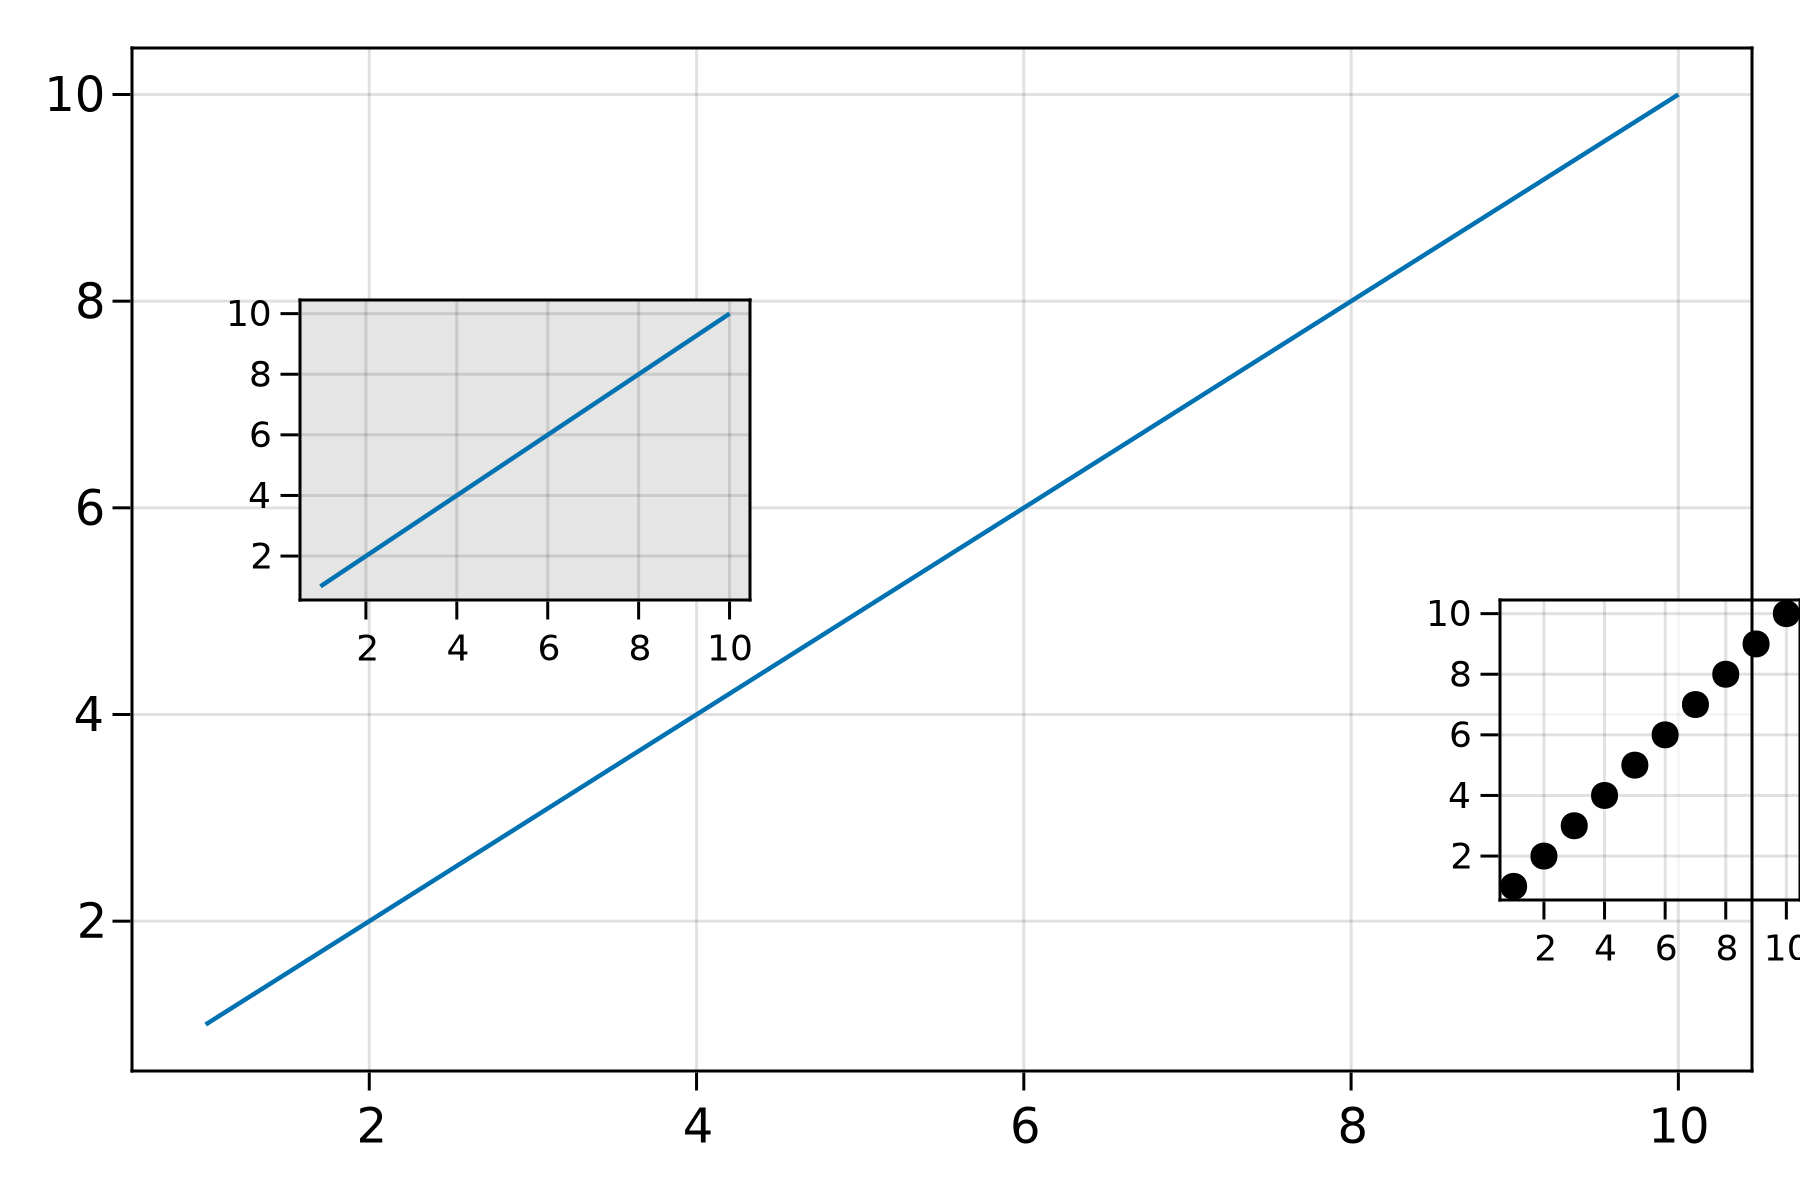
\includegraphics[width=0.6\textwidth,height=\textheight]{_build/im/JDS_figure_box_inset_.png}
\caption{Figure box inset.}\label{fig:figure_box_inset}
}
\end{figure}

其中 \passthrough{\lstinline!Box!} 的尺寸受到
\passthrough{\lstinline!Figure!}中 \passthrough{\lstinline!resolution!}
参数的约束。 注意,也可以在 \passthrough{\lstinline!Axis!} 外绘制插图。
另一种绘制插图的方法是,在位置\passthrough{\lstinline!fig[i, j]!}处定义一个新的
\passthrough{\lstinline!Axis!},并且指定
\passthrough{\lstinline!width!}, \passthrough{\lstinline!height!},
\passthrough{\lstinline!halign!} 和 \passthrough{\lstinline!valign!}。
如下面的函数例子所示:

\begin{lstlisting}[language=Julia]
function add_axis_inset(; pos=fig[1, 1], halign=0.1, valign=0.5,
    width=Relative(0.5), height=Relative(0.35), bgcolor=:lightgray)
    inset_box = Axis(pos, width=width, height=height,
        halign=halign, valign=valign, xticklabelsize=12, yticklabelsize=12,
        backgroundcolor=bgcolor)
    # bring content upfront
    translate!(inset_box.scene, 0, 0, 10)
    elements = keys(inset_box.elements)
    filtered = filter(ele -> ele != :xaxis && ele != :yaxis, elements)
    foreach(ele -> translate!(inset_box.elements[ele], 0, 0, 9), filtered)
    return inset_box
end
\end{lstlisting}

在下面的例子中,如果总图的大小发生变化,那么将重新缩放灰色背景的
\passthrough{\lstinline!Axis!}。 同时 \textbf{插图} 要受到
\passthrough{\lstinline!Axis!} 位置的约束。

\begin{lstlisting}[language=Julia]
function figure_axis_inset()
    fig = Figure(resolution=(600, 400))
    ax = Axis(fig[1, 1], backgroundcolor=:white)
    inset_ax1 = add_axis_inset(; pos=fig[1, 1], halign=0.1, valign=0.65,
        width=Relative(0.3), height=Relative(0.3), bgcolor=:grey90)
    inset_ax2 = add_axis_inset(; pos=fig[1, 1], halign=1, valign=0.25,
        width=Relative(0.25), height=Relative(0.3), bgcolor=(:white, 0.65))
    lines!(ax, 1:10)
    lines!(inset_ax1, 1:10)
    scatter!(inset_ax2, 1:10, color=:black)
    fig
end
figure_axis_inset()
\end{lstlisting}

\begin{figure}
\hypertarget{fig:figure_axis_inset}{%
\centering
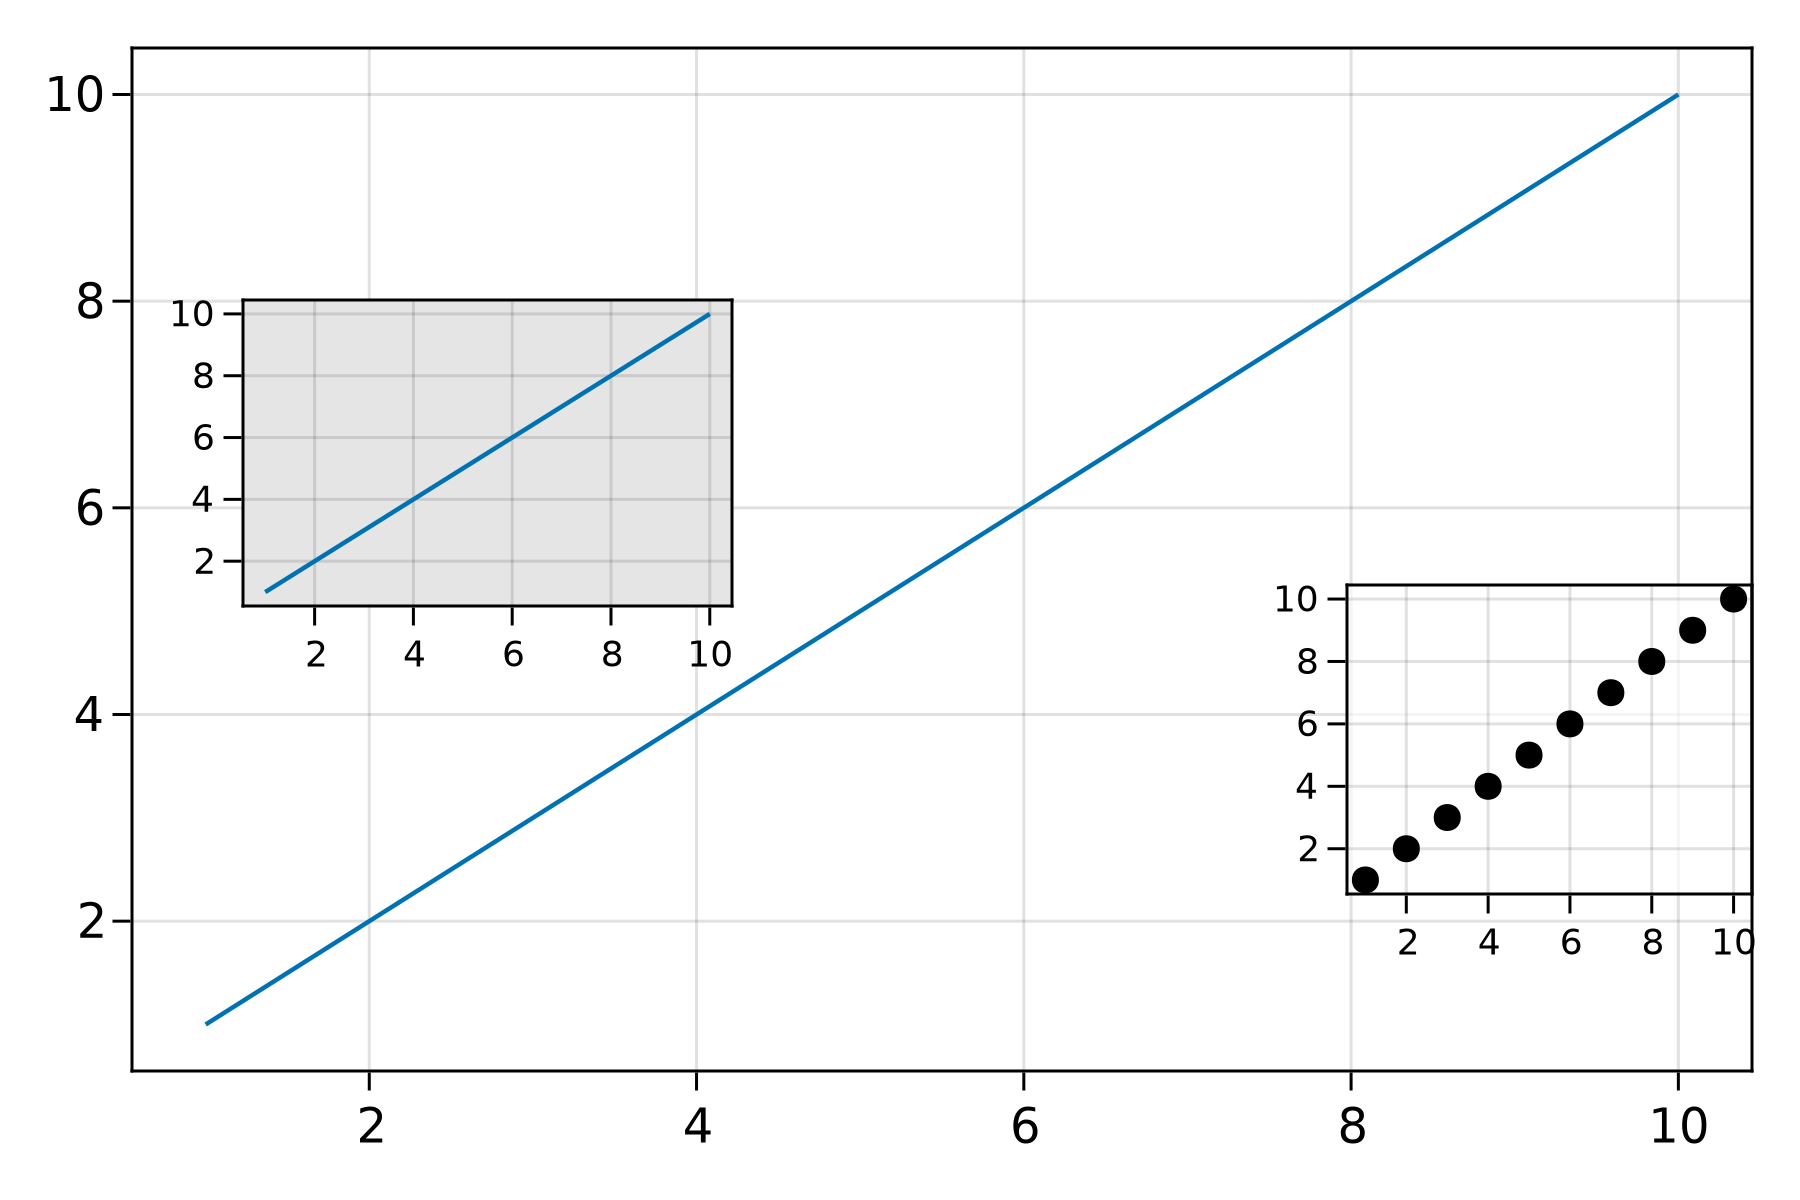
\includegraphics[width=0.6\textwidth,height=\textheight]{_build/im/JDS_figure_axis_inset_.png}
\caption{Figure axis inset.}\label{fig:figure_axis_inset}
}
\end{figure}

以上包含了 Makie 中布局选项的大多数常见用例。 现在,让我们接下来使用
\passthrough{\lstinline!GLMakie.jl!} 绘制一些漂亮的3D示例图。

\hypertarget{sec:glmakie}{%
\section{GLMakie.jl}\label{sec:glmakie}}

\passthrough{\lstinline!CairoMakie.jl!} 满足了所有关于静态 2D 图的需求。
但除此之外,有时候还需要交互性,特别是在处理 3D 图的时候。 使用 3D
图可视化数据是 \textbf{洞察} 数据的常见做法。 这就是
\passthrough{\lstinline!GLMakie.jl!} 的用武之地,它使用
\href{http://www.opengl.org/}{OpenGL} 作为添加交互和响应功能的绘图后端。
与之前一样,一幅简单的图只包括线和点。因此,接下来将从简单图开始。因为已经知道布局如何使用,所以将在例子中应用一些布局。

\hypertarget{ux6563ux70b9ux56feux548cux6298ux7ebfux56fe}{%
\subsection{散点图和折线图}\label{ux6563ux70b9ux56feux548cux6298ux7ebfux56fe}}

散点图有两种绘制选项,第一种是
\passthrough{\lstinline!scatter(x, y, z)!},另一种是
\passthrough{\lstinline!meshscatter(x, y, z)!}。
若使用第一种,标记则不会沿着坐标轴缩放,但在使用第二种时标记会缩放,
这是因为此时它们是三维空间的几何实体。 例子如下:

\begin{lstlisting}
using GLMakie
GLMakie.activate!()
\end{lstlisting}

\begin{lstlisting}[language=Julia]
function scatters_in_3D()
    seed!(123)
    xyz = randn(10, 3)
    x, y, z = xyz[:, 1], xyz[:, 2], xyz[:, 3]
    fig = Figure(resolution=(1600, 400))
    ax1 = Axis3(fig[1, 1]; aspect=(1, 1, 1), perspectiveness=0.5)
    ax2 = Axis3(fig[1, 2]; aspect=(1, 1, 1), perspectiveness=0.5)
    ax3 = Axis3(fig[1, 3]; aspect=:data, perspectiveness=0.5)
    scatter!(ax1, x, y, z; markersize=50)
    meshscatter!(ax2, x, y, z; markersize=0.25)
    hm = meshscatter!(ax3, x, y, z; markersize=0.25,
        marker=FRect3D(Vec3f(0), Vec3f(1)), color=1:size(xyz)[2],
        colormap=:plasma, transparency=false)
    Colorbar(fig[1, 4], hm, label="values", height=Relative(0.5))
    fig
end
scatters_in_3D()
\end{lstlisting}

\begin{figure}
\hypertarget{fig:scatters_in_3D}{%
\centering
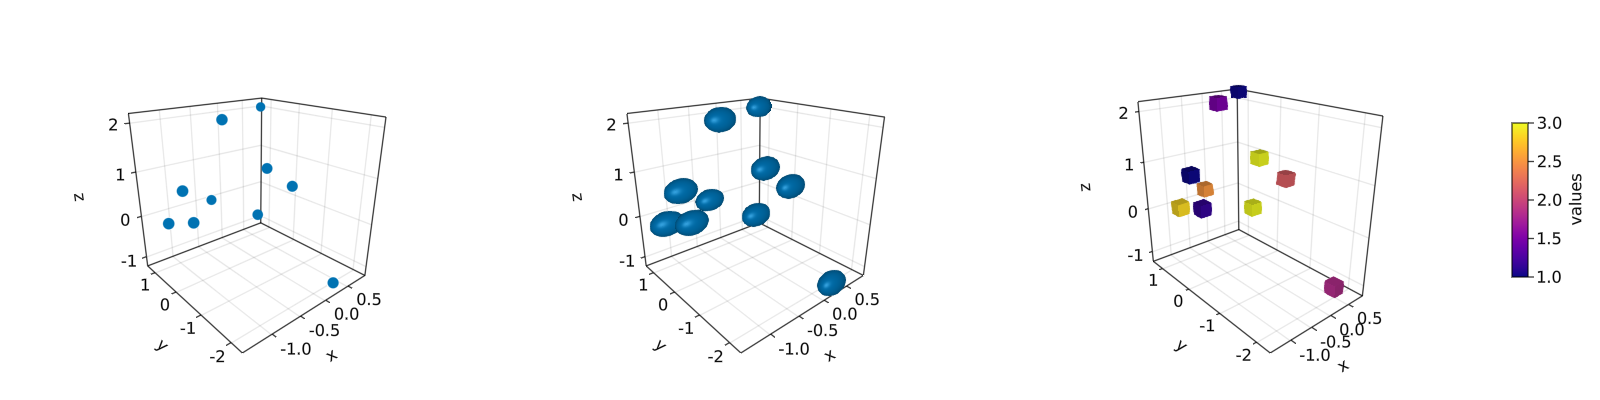
\includegraphics{_build/im/JDS_scatters_in_3D_.png}
\caption{Scatters in 3D.}\label{fig:scatters_in_3D}
}
\end{figure}

另请注意,标记可以是不同的几何实体,比如正方形或矩形。另外,也可以为标记设置
\passthrough{\lstinline!colormap!}。 对于上面位于中间的 3D
图,如果想得到获得完美的球体,那么只需如右侧图那样添加
\passthrough{\lstinline!aspect = :data!} 参数。 绘制
\passthrough{\lstinline!lines!} 或
\passthrough{\lstinline!scatterlines!} 也很简单:

\begin{lstlisting}[language=Julia]
function lines_in_3D()
    seed!(123)
    xyz = randn(10, 3)
    x, y, z = xyz[:, 1], xyz[:, 2], xyz[:, 3]
    fig = Figure(resolution=(1600, 400))
    ax1 = Axis3(fig[1, 1]; aspect=(1, 1, 1), perspectiveness=0.5)
    ax2 = Axis3(fig[1, 2]; aspect=(1, 1, 1), perspectiveness=0.5)
    ax3 = Axis3(fig[1, 3]; aspect=:data, perspectiveness=0.5)
    lines!(ax1, x, y, z; color=1:size(xyz)[2], linewidth=3)
    scatterlines!(ax2, x, y, z; markersize=50)
    hm = meshscatter!(ax3, x, y, z; markersize=0.2, color=1:size(xyz)[2])
    lines!(ax3, x, y, z; color=1:size(xyz)[2])
    Colorbar(fig[2, 1], hm; label="values", height=15, vertical=false,
        flipaxis=false, ticksize=15, tickalign=1, width=Relative(3.55 / 4))
    fig
end
lines_in_3D()
\end{lstlisting}

\begin{figure}
\hypertarget{fig:lines_in_3D}{%
\centering
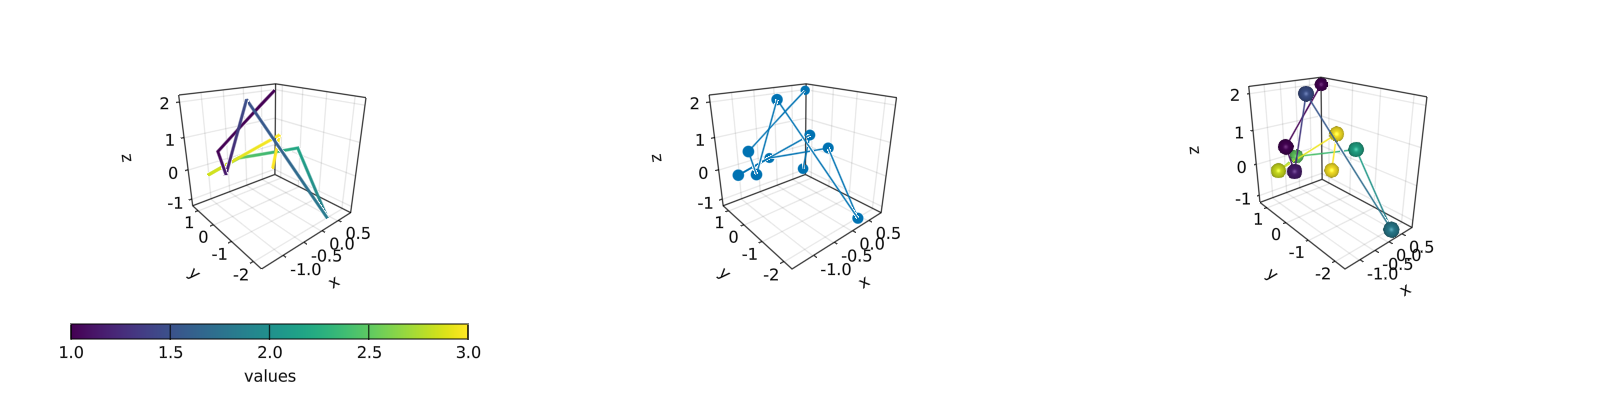
\includegraphics{_build/im/JDS_lines_in_3D_.png}
\caption{Lines in 3D.}\label{fig:lines_in_3D}
}
\end{figure}

在 3D 图中绘制 \passthrough{\lstinline!surface!},
\passthrough{\lstinline!wireframe!} 和 \passthrough{\lstinline!contour!}
是一项容易的工作。

\hypertarget{surfacewireframecontourcontourf-ux548c-contour3d}{%
\subsection{\texorpdfstring{\texttt{surface},\texttt{wireframe},\texttt{contour},\texttt{contourf}
和
\texttt{contour3d}}{surface,wireframe,contour,contourf 和 contour3d}}\label{surfacewireframecontourcontourf-ux548c-contour3d}}

将使用如下的 \passthrough{\lstinline!peaks!} 函数展示这些例子:

\begin{lstlisting}[language=Julia]
function peaks(; n=49)
    x = LinRange(-3, 3, n)
    y = LinRange(-3, 3, n)
    a = 3 * (1 .- x') .^ 2 .* exp.(-(x' .^ 2) .- (y .+ 1) .^ 2)
    b = 10 * (x' / 5 .- x' .^ 3 .- y .^ 5) .* exp.(-x' .^ 2 .- y .^ 2)
    c = 1 / 3 * exp.(-(x' .+ 1) .^ 2 .- y .^ 2)
    return (x, y, a .- b .- c)
end
\end{lstlisting}

不同绘图函数的输出如下:

\begin{lstlisting}[language=Julia]
function plot_peaks_function()
    x, y, z = peaks()
    x2, y2, z2 = peaks(; n=15)
    fig = Figure(resolution=(1600, 400), fontsize=26)
    axs = [Axis3(fig[1, i]; aspect=(1, 1, 1)) for i = 1:3]
    hm = surface!(axs[1], x, y, z)
    wireframe!(axs[2], x2, y2, z2)
    contour3d!(axs[3], x, y, z; levels=20)
    Colorbar(fig[1, 4], hm, height=Relative(0.5))
    fig
end
plot_peaks_function()
\end{lstlisting}

\begin{figure}
\hypertarget{fig:plot_peaks_function}{%
\centering
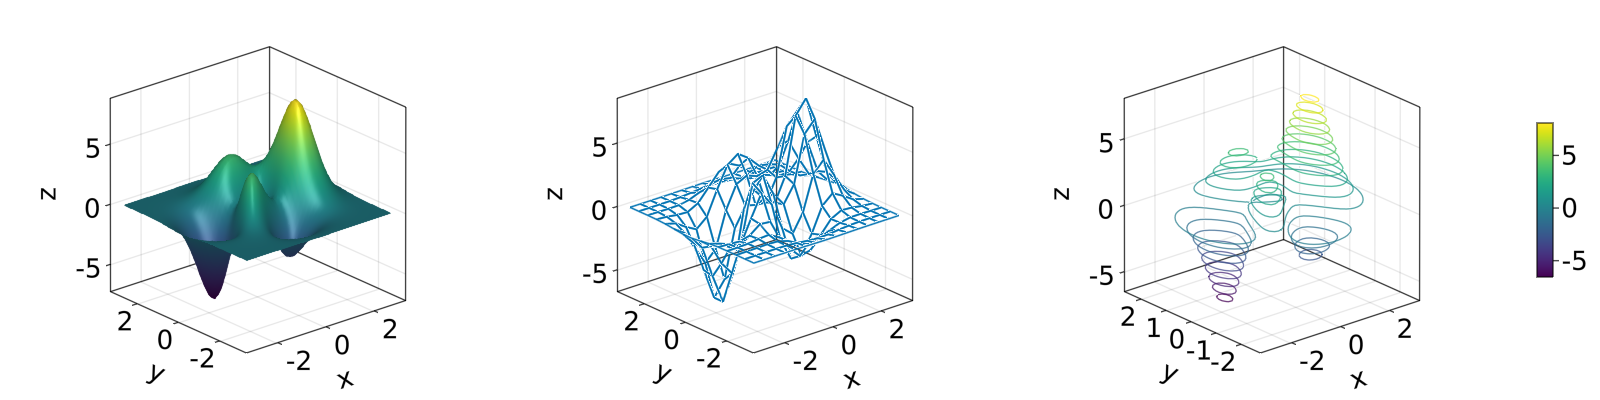
\includegraphics{_build/im/JDS_plot_peaks_function_.png}
\caption{Plot peaks function.}\label{fig:plot_peaks_function}
}
\end{figure}

但是也可以使用
\passthrough{\lstinline!heatmap(x, y, z)!},\passthrough{\lstinline!contour(x, y, z)!}
或 \passthrough{\lstinline!contourf(x, y, z)!} 绘图:

\begin{lstlisting}[language=Julia]
function heatmap_contour_and_contourf()
    x, y, z = peaks()
    fig = Figure(resolution=(1600, 400), fontsize=26)
    axs = [Axis(fig[1, i]; aspect=DataAspect()) for i = 1:3]
    hm = heatmap!(axs[1], x, y, z)
    contour!(axs[2], x, y, z; levels=20)
    contourf!(axs[3], x, y, z)
    Colorbar(fig[1, 4], hm, height=Relative(0.5))
    fig
end
heatmap_contour_and_contourf()
\end{lstlisting}

\begin{figure}
\hypertarget{fig:heatmap_contour_and_contourf}{%
\centering
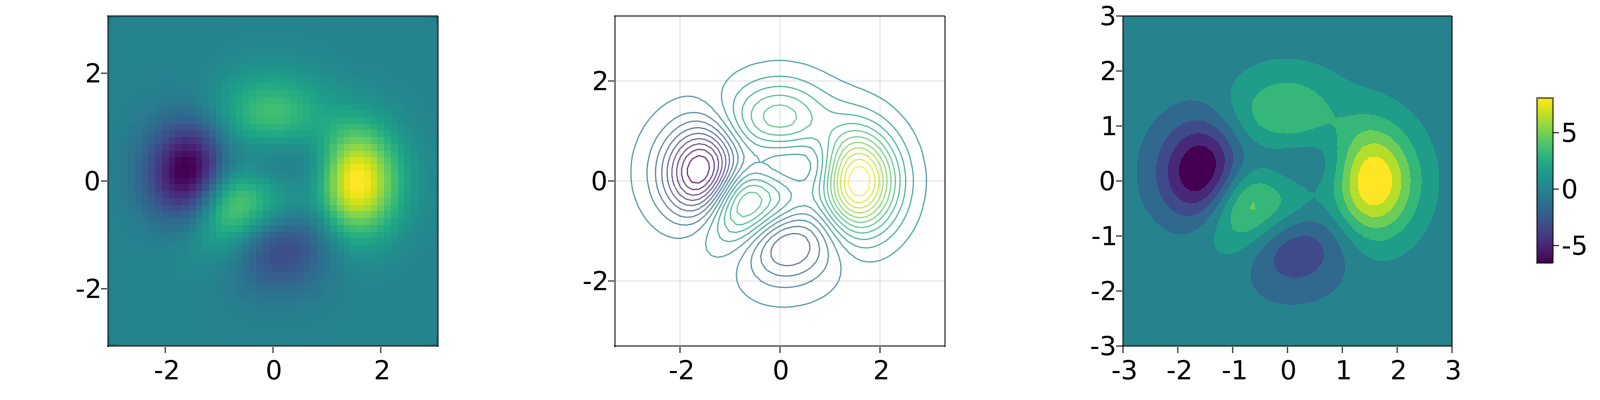
\includegraphics{_build/im/JDS_heatmap_contour_and_contourf_.png}
\caption{Heatmap contour and
contourf.}\label{fig:heatmap_contour_and_contourf}
}
\end{figure}

另外,只要将\passthrough{\lstinline!Axis!} 更改为
\passthrough{\lstinline!Axis3!},这些图就会自动位于 x-y 平面:

\begin{lstlisting}[language=Julia]
function heatmap_contour_and_contourf_in_a_3d_plane()
    x, y, z = peaks()
    fig = Figure(resolution=(1600, 400), fontsize=26)
    axs = [Axis3(fig[1, i]) for i = 1:3]
    hm = heatmap!(axs[1], x, y, z)
    contour!(axs[2], x, y, z; levels=20)
    contourf!(axs[3], x, y, z)
    Colorbar(fig[1, 4], hm, height=Relative(0.5))
    fig
end
heatmap_contour_and_contourf_in_a_3d_plane()
\end{lstlisting}

\begin{figure}
\hypertarget{fig:heatmap_contour_and_contourf_in_a_3d_plane}{%
\centering
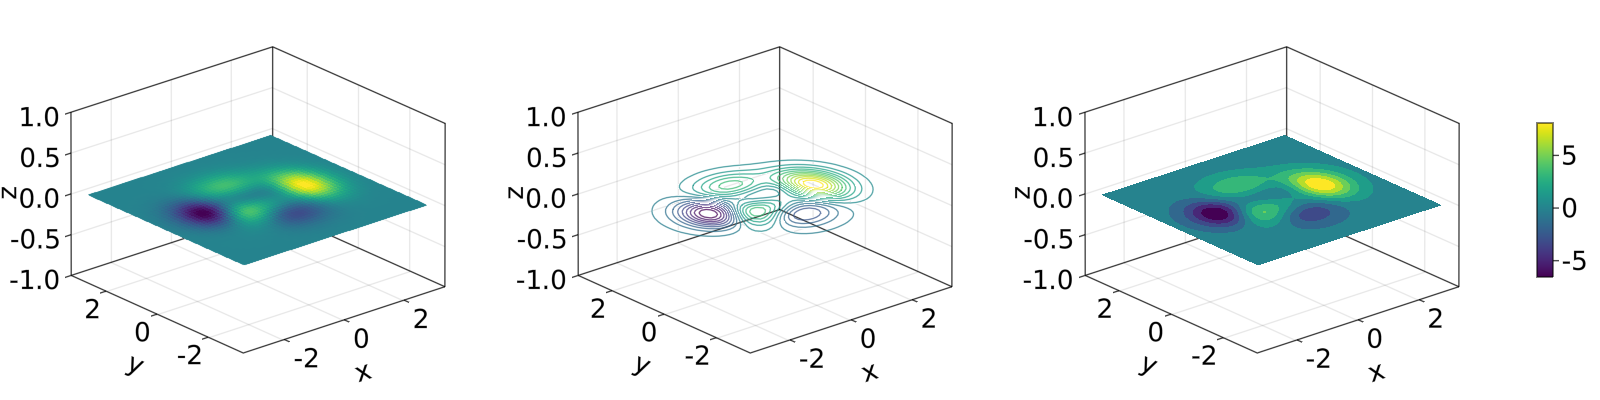
\includegraphics{_build/im/JDS_heatmap_contour_and_contourf_in_a_3d_plane_.png}
\caption{Heatmap contour and contourf in a 3d
plane.}\label{fig:heatmap_contour_and_contourf_in_a_3d_plane}
}
\end{figure}

将这些绘图函数混合在一起也是非常简单的,如下所示:

\begin{lstlisting}
using TestImages
\end{lstlisting}

\begin{lstlisting}[language=Julia]
function mixing_surface_contour3d_contour_and_contourf()
    img = testimage("coffee.png")
    x, y, z = peaks()
    cmap = :Spectral_11
    fig = Figure(resolution=(1200, 800), fontsize=26)
    ax1 = Axis3(fig[1, 1]; aspect=(1, 1, 1), elevation=pi / 6, xzpanelcolor=(:black, 0.75),
        perspectiveness=0.5, yzpanelcolor=:black, zgridcolor=:grey70,
        ygridcolor=:grey70, xgridcolor=:grey70)
    ax2 = Axis3(fig[1, 3]; aspect=(1, 1, 1), elevation=pi / 6, perspectiveness=0.5)
    hm = surface!(ax1, x, y, z; colormap=(cmap, 0.95), shading=true)
    contour3d!(ax1, x, y, z .+ 0.02; colormap=cmap, levels=20, linewidth=2)
    xmin, ymin, zmin = minimum(ax1.finallimits[])
    xmax, ymax, zmax = maximum(ax1.finallimits[])
    contour!(ax1, x, y, z; colormap=cmap, levels=20, transformation=(:xy, zmax))
    contourf!(ax1, x, y, z; colormap=cmap, transformation=(:xy, zmin))
    Colorbar(fig[1, 2], hm, width=15, ticksize=15, tickalign=1, height=Relative(0.35))
    # transformations into planes
    heatmap!(ax2, x, y, z; colormap=:viridis, transformation=(:yz, 3.5))
    contourf!(ax2, x, y, z; colormap=:CMRmap, transformation=(:xy, -3.5))
    contourf!(ax2, x, y, z; colormap=:bone_1, transformation=(:xz, 3.5))
    image!(ax2, -3 .. 3, -3 .. 2, rotr90(img); transformation=(:xy, 3.8))
    xlims!(ax2, -3.8, 3.8)
    ylims!(ax2, -3.8, 3.8)
    zlims!(ax2, -3.8, 3.8)
    fig
end
mixing_surface_contour3d_contour_and_contourf()
\end{lstlisting}

\begin{figure}
\hypertarget{fig:mixing_surface_contour3d_contour_and_contourf}{%
\centering
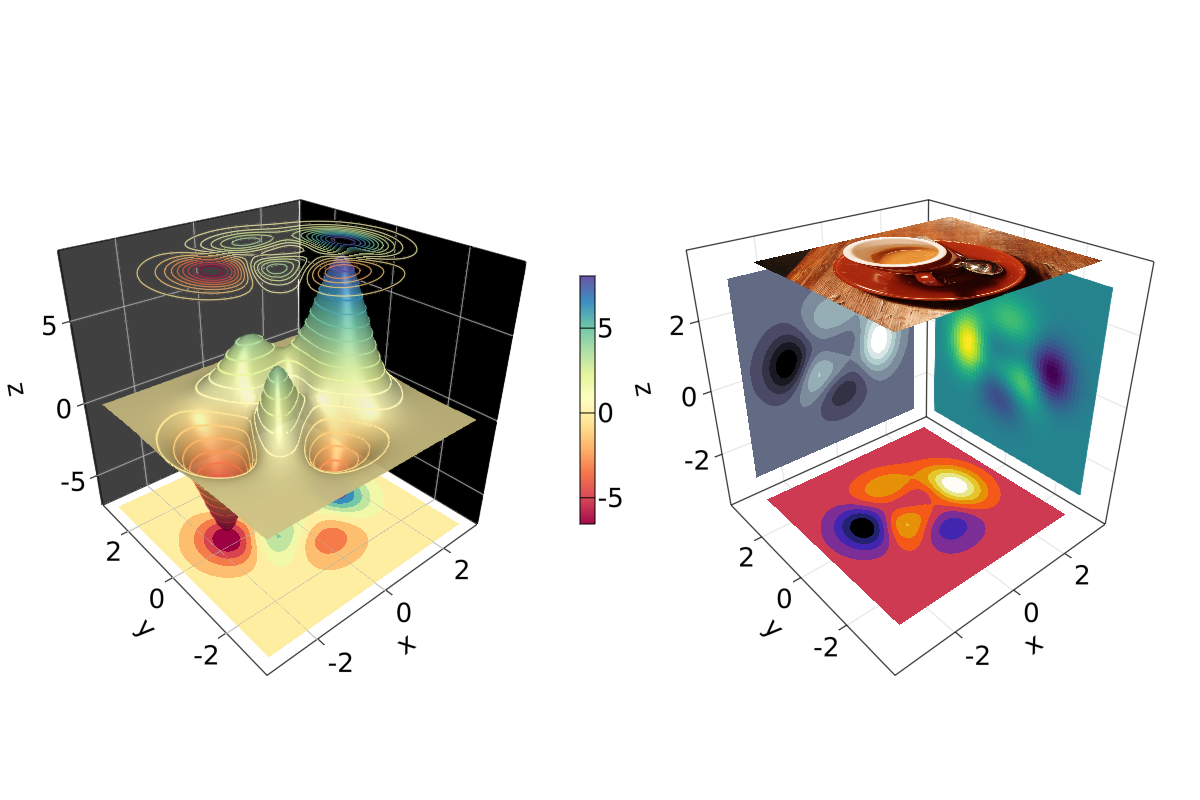
\includegraphics[width=0.6\textwidth,height=\textheight]{_build/im/JDS_mixing_surface_contour3d_contour_and_contourf_.png}
\caption{Mixing surface, contour3d, contour and
contourf.}\label{fig:mixing_surface_contour3d_contour_and_contourf}
}
\end{figure}

还不错,对吧?从这里也可以看出,任何的
\passthrough{\lstinline!heatmap!},
\passthrough{\lstinline!contour!},\passthrough{\lstinline!contourf!} 和
\passthrough{\lstinline!image!} 都可以绘制在任何平面上。

\hypertarget{arrows-ux548c-streamplot}{%
\subsection{\texorpdfstring{\texttt{arrows} 和
\texttt{streamplot}}{arrows 和 streamplot}}\label{arrows-ux548c-streamplot}}

当想要知道给定变量的方向时,\passthrough{\lstinline!arrows!} 和
\passthrough{\lstinline!streamplot!} 会变得非常有用。
参见如下的示例\footnote{此处使用 Julia 标准库中的
  \passthrough{\lstinline!LinearAlgebra!}。}:

\begin{lstlisting}
using LinearAlgebra
\end{lstlisting}

\begin{lstlisting}[language=Julia]
function arrows_and_streamplot_in_3d()
    ps = [Point3f(x, y, z) for x = -3:1:3 for y = -3:1:3 for z = -3:1:3]
    ns = map(p -> 0.1 * rand() * Vec3f(p[2], p[3], p[1]), ps)
    lengths = norm.(ns)
    flowField(x, y, z) = Point(-y + x * (-1 + x^2 + y^2)^2, x + y * (-1 + x^2 + y^2)^2,
        z + x * (y - z^2))
    fig = Figure(resolution=(1200, 800), fontsize=26)
    axs = [Axis3(fig[1, i]; aspect=(1, 1, 1), perspectiveness=0.5) for i = 1:2]
    arrows!(axs[1], ps, ns, color=lengths, arrowsize=Vec3f0(0.2, 0.2, 0.3),
        linewidth=0.1)
    streamplot!(axs[2], flowField, -4 .. 4, -4 .. 4, -4 .. 4, colormap=:plasma,
        gridsize=(7, 7), arrow_size=0.25, linewidth=1)
    fig
end
arrows_and_streamplot_in_3d()
\end{lstlisting}

\begin{figure}
\hypertarget{fig:arrows_and_streamplot_in_3d}{%
\centering
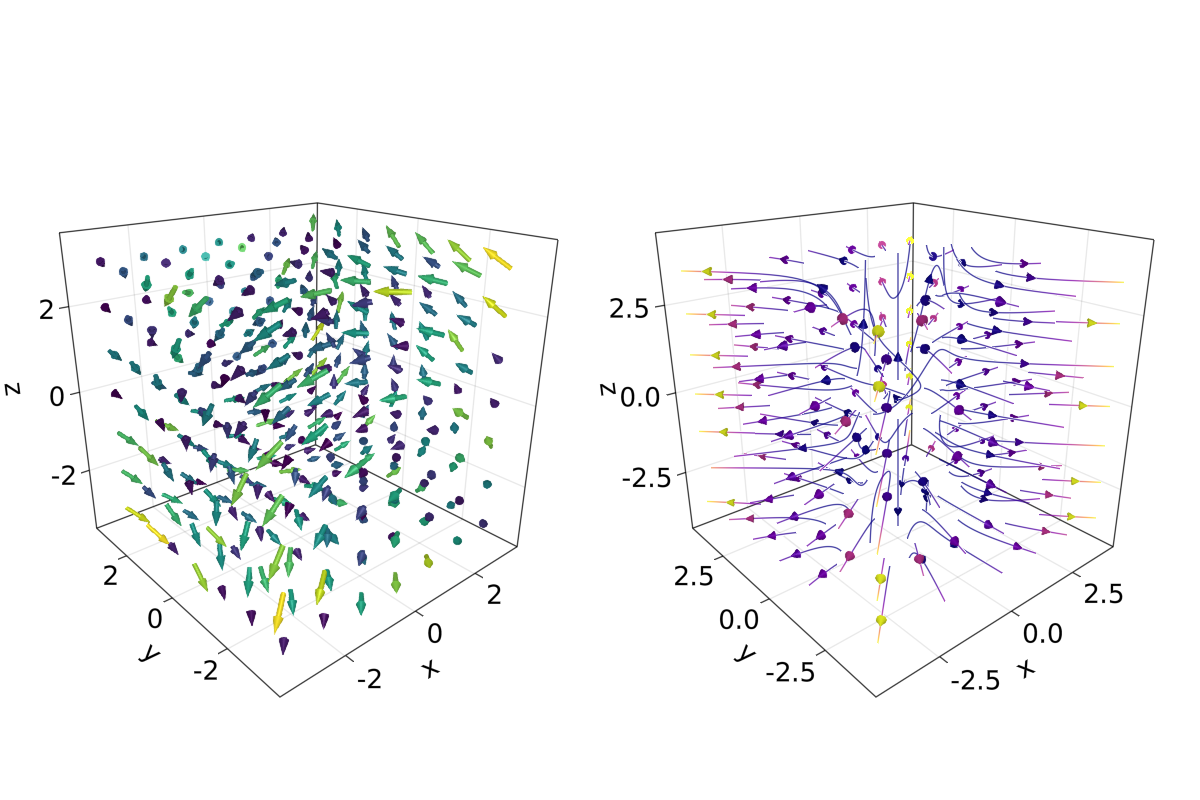
\includegraphics[width=0.6\textwidth,height=\textheight]{_build/im/JDS_arrows_and_streamplot_in_3d_.png}
\caption{Arrows and streamplot in
3d.}\label{fig:arrows_and_streamplot_in_3d}
}
\end{figure}

另外一些有趣的例子是
\passthrough{\lstinline!mesh(obj)!},\passthrough{\lstinline!volume(x, y, z, vals)!}
和 \passthrough{\lstinline!contour(x, y, z, vals)!}。

\hypertarget{mesh-ux548c-volume}{%
\subsection{\texorpdfstring{\texttt{mesh} 和
\texttt{volume}}{mesh 和 volume}}\label{mesh-ux548c-volume}}

绘制网格在想要画出几何实体时很有用,例如
\passthrough{\lstinline!Sphere!} 或矩形这样的几何实体,即
\passthrough{\lstinline!FRect3D!}。 另一种在 3D 空间中可视化的方法是调用
\passthrough{\lstinline!volume!} 和 \passthrough{\lstinline!contour!}
函数,它们通过实现
\href{https://en.wikipedia.org/wiki/Ray_tracing_(graphics)}{光线追踪}
来模拟各种光学效果。 例子如下:

\begin{lstlisting}
using GeometryBasics
\end{lstlisting}

\begin{lstlisting}[language=Julia]
function mesh_volume_contour()
    # mesh objects
    rectMesh = FRect3D(Vec3f(-0.5), Vec3f(1))
    recmesh = GeometryBasics.mesh(rectMesh)
    sphere = Sphere(Point3f(0), 1)
    # https://juliageometry.github.io/GeometryBasics.jl/stable/primitives/
    spheremesh = GeometryBasics.mesh(Tesselation(sphere, 64))
    # uses 64 for tesselation, a smoother sphere
    colors = [rand() for v in recmesh.position]
    # cloud points for volume
    x = y = z = 1:10
    vals = randn(10, 10, 10)
    fig = Figure(resolution=(1600, 400))
    axs = [Axis3(fig[1, i]; aspect=(1, 1, 1), perspectiveness=0.5) for i = 1:3]
    mesh!(axs[1], recmesh; color=colors, colormap=:rainbow, shading=false)
    mesh!(axs[1], spheremesh; color=(:white, 0.25), transparency=true)
    volume!(axs[2], x, y, z, vals; colormap=Reverse(:plasma))
    contour!(axs[3], x, y, z, vals; colormap=Reverse(:plasma))
    fig
end
mesh_volume_contour()
\end{lstlisting}

\begin{figure}
\hypertarget{fig:mesh_volume_contour}{%
\centering
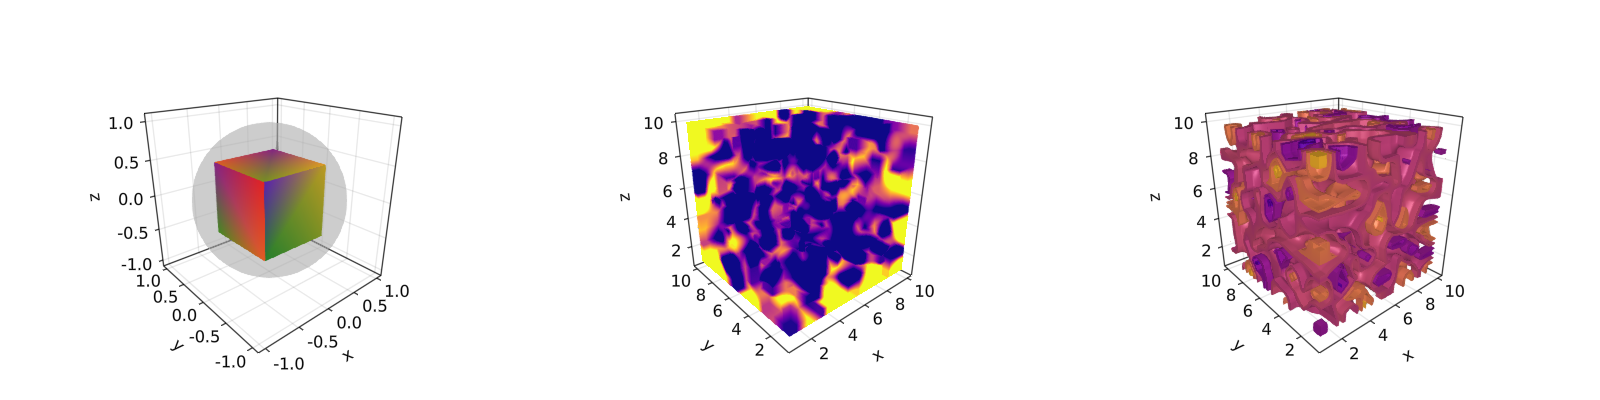
\includegraphics{_build/im/JDS_mesh_volume_contour_.png}
\caption{Mesh volume contour.}\label{fig:mesh_volume_contour}
}
\end{figure}

注意到透明球和立方体绘制在同一个坐标系中。 截至目前,我们已经包含了 3D
绘图的大多数用例。 另一个例子是
\passthrough{\lstinline!?linesegments!}。

参考之前的例子,可以使用球体和矩形平面创建一些自定义图:

\begin{lstlisting}
using GeometryBasics, Colors
\end{lstlisting}

首先为球体定义一个矩形网格,而且给每个球定义不同的颜色。
另外,可以将球体和平面混合在一张图里。下面的代码定义了所有必要的数据。

\begin{lstlisting}[language=Julia]
seed!(123)
spheresGrid = [Point3f(i,j,k) for i in 1:2:10 for j in 1:2:10 for k in 1:2:10]
colorSphere = [RGBA(i * 0.1, j * 0.1, k * 0.1, 0.75) for i in 1:2:10 for j in 1:2:10 for k in 1:2:10]
spheresPlane = [Point3f(i,j,k) for i in 1:2.5:20 for j in 1:2.5:10 for k in 1:2.5:4]
cmap = get(colorschemes[:plasma], LinRange(0, 1, 50))
colorsPlane = cmap[rand(1:50,50)]
rectMesh = FRect3D(Vec3f(-1, -1, 2.1), Vec3f(22, 11, 0.5))
recmesh = GeometryBasics.mesh(rectMesh)
colors = [RGBA(rand(4)...) for v in recmesh.position]
\end{lstlisting}

然后可使用如下方式简单地绘图:

\begin{lstlisting}[language=Julia]
function grid_spheres_and_rectangle_as_plate()
    fig = with_theme(theme_dark()) do
        fig = Figure(resolution=(1200, 800))
        ax1 = Axis3(fig[1, 1]; aspect=:data, perspectiveness=0.5, azimuth=0.72)
        ax2 = Axis3(fig[1, 2]; aspect=:data, perspectiveness=0.5)
        meshscatter!(ax1, spheresGrid; color = colorSphere, markersize = 1,
            shading=false)
        meshscatter!(ax2, spheresPlane; color=colorsPlane, markersize = 0.75,
            lightposition=Vec3f(10, 5, 2), ambient=Vec3f(0.95, 0.95, 0.95),
            backlight=1.0f0)
        mesh!(recmesh; color=colors, colormap=:rainbow, shading=false)
        limits!(ax1, 0, 10, 0, 10, 0, 10)
        fig
    end
    fig
end
grid_spheres_and_rectangle_as_plate()
\end{lstlisting}

\begin{figure}
\hypertarget{fig:grid_spheres_and_rectangle_as_plate}{%
\centering
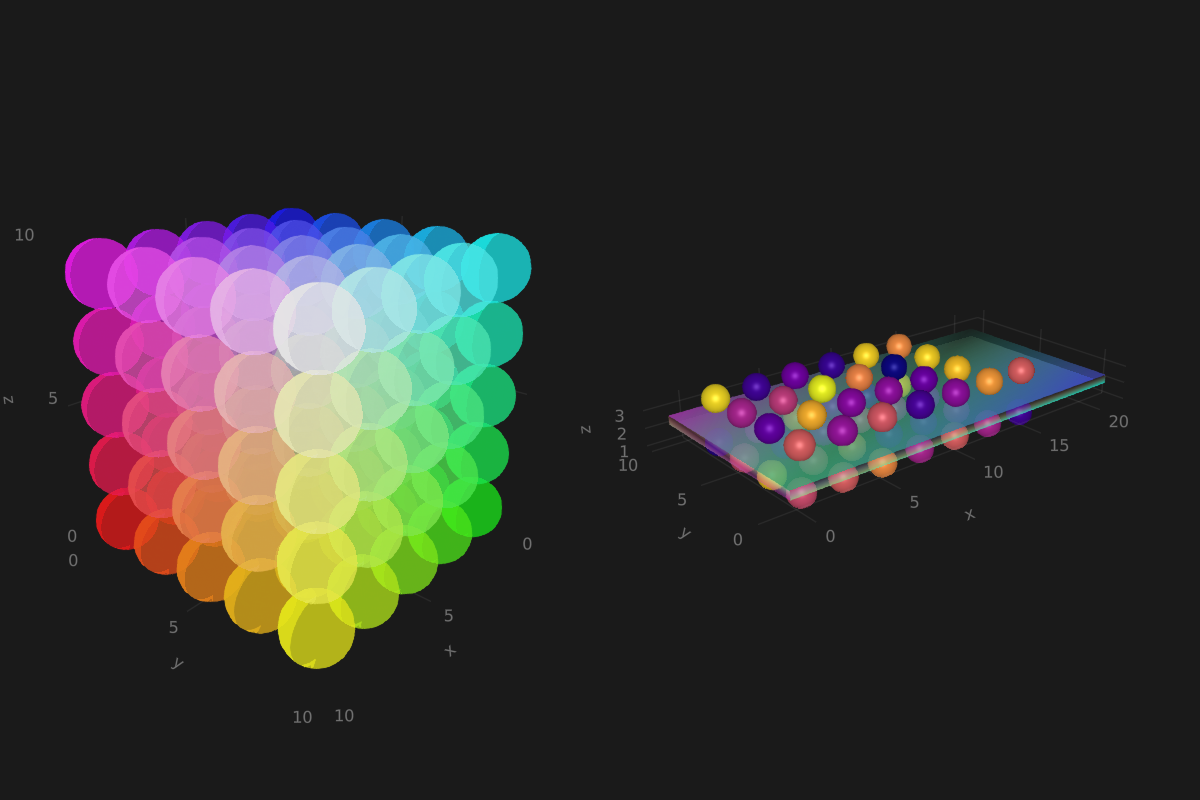
\includegraphics[width=0.6\textwidth,height=\textheight]{_build/im/JDS_grid_spheres_and_rectangle_as_plate_.png}
\caption{Grid spheres and rectangle as
plate.}\label{fig:grid_spheres_and_rectangle_as_plate}
}
\end{figure}

注意,右侧图中的矩形平面是半透明的,这是因为颜色函数
\passthrough{\lstinline!RGBA()!} 中定义了
\passthrough{\lstinline!alpha!} 参数。
矩形函数是通用的,因此很容易用来实现 3D 方块,而它又能用于绘制 3D
直方图。 参见如下的例子,我们将再次使用 \passthrough{\lstinline!peaks!}
函数并增加一些定义:

\begin{lstlisting}[language=Julia]
x, y, z = peaks(; n=15)
δx = (x[2] - x[1]) / 2
δy = (y[2] - y[1]) / 2
cbarPal = :Spectral_11
ztmp = (z .- minimum(z)) ./ (maximum(z .- minimum(z)))
cmap = get(colorschemes[cbarPal], ztmp)
cmap2 = reshape(cmap, size(z))
ztmp2 = abs.(z) ./ maximum(abs.(z)) .+ 0.15
\end{lstlisting}

其中方块的尺寸由 \(\delta x, \delta y\) 指定。
\passthrough{\lstinline!cmap2!} 用于指定每个方块的颜色而
\passthrough{\lstinline!ztmp2!} 用于指定每个方块的透明度。如下图所示。

\begin{lstlisting}[language=Julia]
function histogram_or_bars_in_3d()
    fig = Figure(resolution=(1200, 800), fontsize=26)
    ax1 = Axis3(fig[1, 1]; aspect=(1, 1, 1), elevation=π/6,
        perspectiveness=0.5)
    ax2 = Axis3(fig[1, 2]; aspect=(1, 1, 1), perspectiveness=0.5)
    rectMesh = FRect3D(Vec3f0(-0.5, -0.5, 0), Vec3f0(1, 1, 1))
    meshscatter!(ax1, x, y, 0*z, marker = rectMesh, color = z[:],
        markersize = Vec3f.(2δx, 2δy, z[:]), colormap = :Spectral_11,
        shading=false)
    limits!(ax1, -3.5, 3.5, -3.5, 3.5, -7.45, 7.45)
    meshscatter!(ax2, x, y, 0*z, marker = rectMesh, color = z[:],
        markersize = Vec3f.(2δx, 2δy, z[:]), colormap = (:Spectral_11, 0.25),
        shading=false, transparency=true)
    for (idx, i) in enumerate(x), (idy, j) in enumerate(y)
        rectMesh = FRect3D(Vec3f(i - δx, j - δy, 0), Vec3f(2δx, 2δy, z[idx, idy]))
        recmesh = GeometryBasics.mesh(rectMesh)
        lines!(ax2, recmesh; color=(cmap2[idx, idy], ztmp2[idx, idy]))
    end
    fig
end
histogram_or_bars_in_3d()
\end{lstlisting}

\begin{figure}
\hypertarget{fig:histogram_or_bars_in_3d}{%
\centering
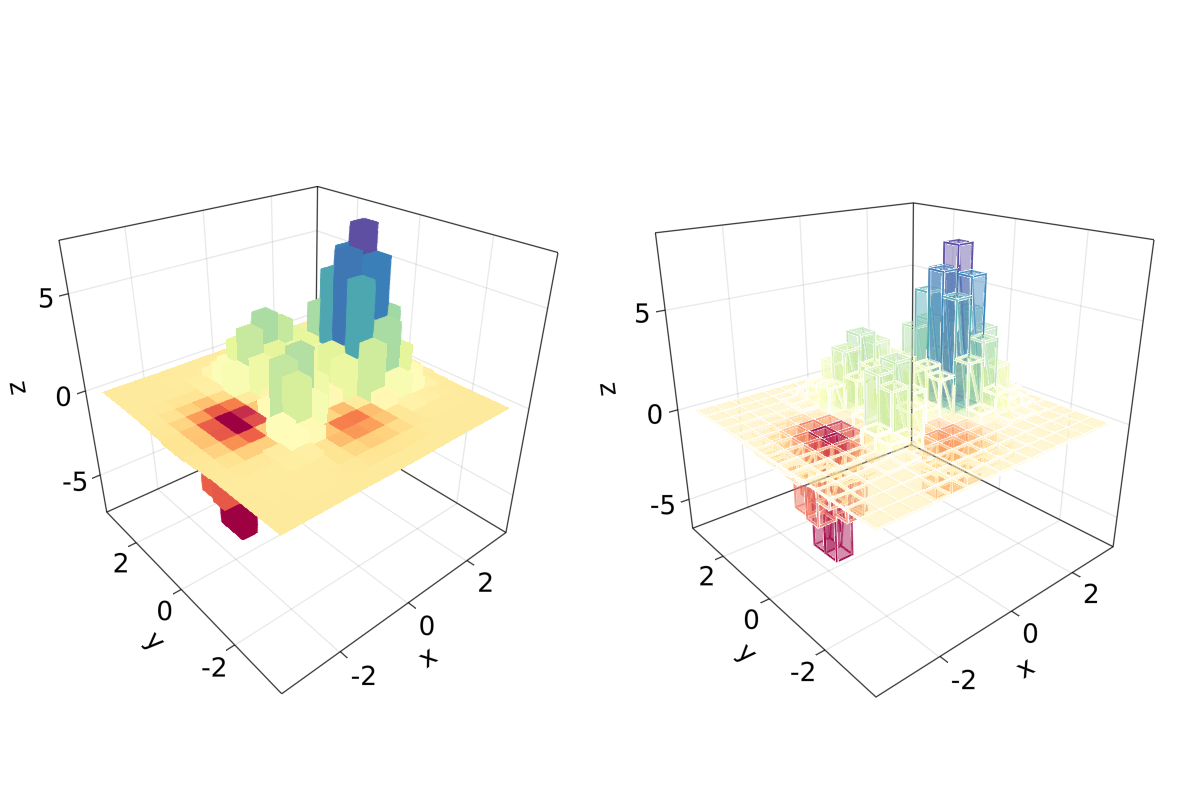
\includegraphics[width=0.6\textwidth,height=\textheight]{_build/im/JDS_histogram_or_bars_in_3d_.png}
\caption{Histogram or bars in 3d.}\label{fig:histogram_or_bars_in_3d}
}
\end{figure}

应注意到,也可以在 \passthrough{\lstinline!mesh!} 对象上调用
\passthrough{\lstinline!lines!} 或 \passthrough{\lstinline!wireframe!}。

\hypertarget{ux586bux5145ux7684ux7ebfux548cux5e26}{%
\subsection{填充的线和带}\label{ux586bux5145ux7684ux7ebfux548cux5e26}}

在最终的例子中, 我们将展示如何使用 \passthrough{\lstinline!band!}和一些
\passthrough{\lstinline!linesegments!} 填充 3D 图中的曲线:

\begin{lstlisting}[language=Julia]
function filled_line_and_linesegments_in_3D()
    xs = LinRange(-3, 3, 10)
    lower = [Point3f(i, -i, 0) for i in LinRange(0, 3, 100)]
    upper = [Point3f(i, -i, sin(i) * exp(-(i + i))) for i in range(0, 3, length=100)]
    fig = Figure(resolution=(1200, 800))
    axs = [Axis3(fig[1, i]; elevation=pi/6, perspectiveness=0.5) for i = 1:2]
    band!(axs[1], lower, upper, color=repeat(norm.(upper), outer=2), colormap=:CMRmap)
    lines!(axs[1], upper, color=:black)
    linesegments!(axs[2], cos.(xs), xs, sin.(xs), linewidth=5, color=1:length(xs))
    fig
end
filled_line_and_linesegments_in_3D()
\end{lstlisting}

\begin{figure}
\hypertarget{fig:filled_line_and_linesegments_in_3D}{%
\centering
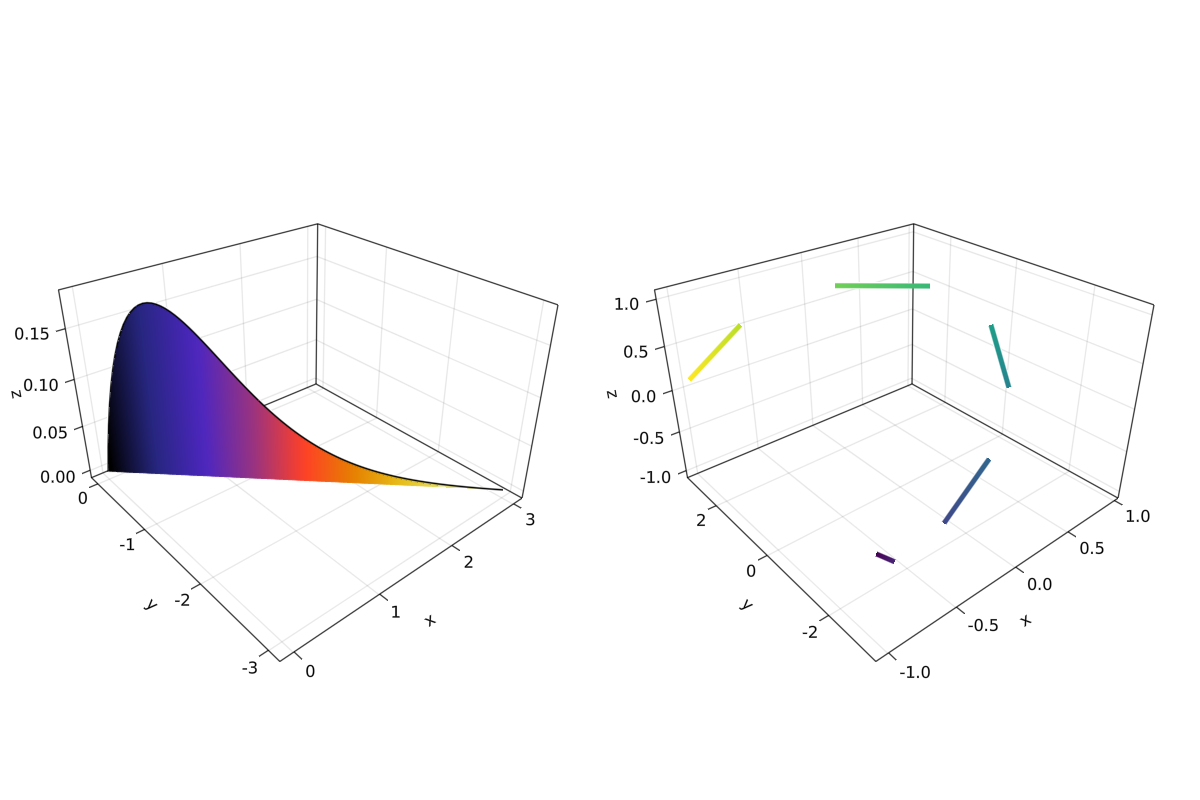
\includegraphics[width=0.6\textwidth,height=\textheight]{_build/im/JDS_filled_line_and_linesegments_in_3D_.png}
\caption{Filled line and linesegments in
3D.}\label{fig:filled_line_and_linesegments_in_3D}
}
\end{figure}

最后,我们的3D绘图之旅到此结束。
你可以将我们这里展示的一切结合起来,去创造令人惊叹的 3D 图!

\hypertarget{sec:appendix}{%
\chapter{附录}\label{sec:appendix}}

\hypertarget{sec:appendix_pkg}{%
\section{库的版本}\label{sec:appendix_pkg}}

本书由 Julia 1.7.3 及以下库构建:

\begin{lstlisting}[language=Julia]
Books 1.2.8
CSV 0.10.14
CairoMakie 0.7.5
CategoricalArrays 0.10.8
ColorSchemes 3.25.0
Colors 0.12.11
DataFrames 1.6.1
Distributions 0.25.109
FileIO 1.16.3
GLMakie 0.5.5
GeometryBasics 0.4.11
ImageMagick 1.3.1
LaTeXStrings 1.3.1
Makie 0.16.6
QuartzImageIO 0.7.4
Reexport 1.2.2
StatsBase 0.33.21
TestImages 1.8.0
XLSX 0.7.10
\end{lstlisting}

Build: 2024-06-04 9:34 UTC

\hypertarget{sec:notation}{%
\section{符号}\label{sec:notation}}

我们尽量保持本书符号的一致性。 这会使阅读和编写代码更容易。
我们可以将符号定义为三个部分。

\hypertarget{sec:julia_style_guide}{%
\subsection{Julia 风格指南}\label{sec:julia_style_guide}}

首先,我们尝试遵循
\href{https://docs.julialang.org/en/v1/manual/style-guide/}{Julia
风格指南} 中的约定惯例。 更重要的是,要编写函数而不是脚本(也可查阅
Section~\ref{sec:engineering})。 另外,我们使用与 Julia
\passthrough{\lstinline!base/!} 模块一致的命名约定,即:

\begin{itemize}
\tightlist
\item
  模块采用驼峰命名法:
  \passthrough{\lstinline!module JuliaDataScience!},
  \passthrough{\lstinline!struct MyPoint!}。
  (之所叫驼峰命名法,是因为单词的首字母大写,如 ``iPad'' 或
  ``CamelCase'', 这使得单词看起来像驼峰。)
\item
  函数名全部小写,并用下划线分隔单词。
  不过也允许在命名函数时省略分隔符。 例如,这些函数名都符合约定:
  \passthrough{\lstinline!my\_function!},
  \passthrough{\lstinline!myfunction!} 和
  \passthrough{\lstinline!string2int!}。
\end{itemize}

同时,避免在条件语句中使用括号,即写为
\passthrough{\lstinline!if a == b!} 而不是
\passthrough{\lstinline!if (a == b)!},并且每级缩进使用 4 个空格。

\hypertarget{sec:blue_style_guide}{%
\subsection{Blue 风格指南}\label{sec:blue_style_guide}}

\href{https://github.com/invenia/BlueStyle}{Blue 风格指南} 在默认的
Julia 风格指南基础上增加了更多的约定。
一些规则可能听起来有点古板,但我们发现这样能提高代码的可读性。

根据风格指南,我们具体坚持:

\begin{itemize}
\item
  每行代码最多 92 字符(Markdown 文件允许更长的行)。
\item
  使用 \passthrough{\lstinline!using!} 加载模块,且每行最多加载一个。
\item
  行尾无空格。
  行尾的空格会使代码更改检查更加困难,因为虽然它们不会修改代码行为,但会显示为更改。
\item
  避免括号内的多余空格。 因此,要写为
  \passthrough{\lstinline!string(1, 2)!} 而不是
  \passthrough{\lstinline!string( 1 , 2 )!}。
\item
  应避免全局变量。
\item
  尝试将函数名压缩至一到两个词。
\item
  使用分号 \passthrough{\lstinline!;!} 来说明参数是否为关键字参数。
  例如,使用 \passthrough{\lstinline!func(x; y=3)!} 而不是
  \passthrough{\lstinline!func(x, y=3)!}。
\item
  避免使用多个空格来对齐对象。 所以,应该写

\begin{lstlisting}
a = 1
lorem = 2
\end{lstlisting}

  而不是

\begin{lstlisting}
a     = 1
lorem = 2
\end{lstlisting}
\item
  当合适时,我们应在双目运算符两侧增加空格,例如,
  \passthrough{\lstinline!1 == 2!} 或
  \passthrough{\lstinline!y = x + 1!}。
\item
  缩进三引号和三反引号:

\begin{lstlisting}
s = """
    my long text:
    [...]
    the end.
    """
\end{lstlisting}
\item
  不要省略浮点数中的零(即使 Julia 允许这样做)。 因此,写为
  \passthrough{\lstinline!1.0!} 而不是 \passthrough{\lstinline!1.!}
  ,写为 \passthrough{\lstinline!0.1!} 而不是
  \passthrough{\lstinline!.1!}。
\item
  在 for 循环中使用 \passthrough{\lstinline!in!},而不是
  \passthrough{\lstinline!=!} 或 \passthrough{\lstinline!∈!} (即使
  Julia 允许这样做)。
\end{itemize}

\hypertarget{ux6211ux4eecux7684ux8865ux5145}{%
\subsection{我们的补充}\label{ux6211ux4eecux7684ux8865ux5145}}

\begin{itemize}
\tightlist
\item
  在行文时,我们将使用 \passthrough{\lstinline!M.foo!} 引用
  \passthrough{\lstinline!M.foo(3, 4)!},而不是使用
  \passthrough{\lstinline!M.foo(...)!} 或
  \passthrough{\lstinline!M.foo()!}。
\item
  当讨论软件包时,如 DataFrames 包,我们每次都会明确地写为
  \passthrough{\lstinline!DataFrames.jl!}。
  这使得可以非常容易地定位正在讨论的包。
\item
  对于文件名, 我们坚持使用 ``file.txt'',而不是
  \passthrough{\lstinline!file.txt!} 或
  file.txt,因为这种形式与代码保持一致。
\item
  对于表中的列,如列 \passthrough{\lstinline!x!},我们坚持使用
  \passthrough{\lstinline!:x!},因为这种形式与代码保持一致。
\item
  不要在行内代码使用 Unicode 符号。 这只是一个 PDF 生成中的
  bug,但现在我们必须解决它。
\item
  每个代码块前面的行以冒号 (:) 结尾,表示此行属于该代码块。
\end{itemize}

\hypertarget{ux52a0ux8f7dux7b26ux53f7}{%
\subsubsection{加载符号}\label{ux52a0ux8f7dux7b26ux53f7}}

在不使用 REPL 时,我们更喜欢显式加载符号,即更喜欢使用
\passthrough{\lstinline!using A: foo!} 而不是
\passthrough{\lstinline!using A!}(另请查阅
\protect\hyperlink{ref-jump2021using}{\emph{JuMP Style Guide}}
(\protect\hyperlink{ref-jump2021using}{2021}))。
在此上下文中,符号表示对象的标识符。 例如,即使看起来不正常, 但本质上
\passthrough{\lstinline!DataFrame!}、\passthrough{\lstinline!π!} 和
\passthrough{\lstinline!CSV!} 都是符号。 在使用诸如
\passthrough{\lstinline!isdefined!} 这样的 Julia
方法时,我们发现了这一点:

\begin{lstlisting}[language=Julia]
isdefined(Main, :π)
\end{lstlisting}

\begin{lstlisting}[language=Output]
true
\end{lstlisting}

接下来使用 \passthrough{\lstinline!using!} 时会变得显式,另外更喜欢使用
\passthrough{\lstinline!using A: foo!} 而不是
\passthrough{\lstinline!import A: foo!} ,因为后者更容易意外地扩展
\passthrough{\lstinline!foo!}。 注意这不仅仅是针对 Julia 的建议: Python
也不鼓励通过 \passthrough{\lstinline!from <module> import *!}
隐式加载符号 (\protect\hyperlink{ref-pep8}{van Rossum et al., 2001})。

显式加载的重要性与语义版本控制有关。 结合语义版本控制
(\url{http://semver.org}) 后,版本号将关系到包是否存在 \textbf{破坏性}
更新。 例如,当包 \passthrough{\lstinline!A!} 的版本号从
\passthrough{\lstinline!0.2.2!} 变化到
\passthrough{\lstinline!0.2.3!},其进行的是非破坏性更新。
在这种非破坏性更新下,你不用担心你的包会产生破坏,即抛出错误或改变行为。
如果包 \passthrough{\lstinline!A!} 从 \passthrough{\lstinline!0.2!}
变化到 \passthrough{\lstinline!1.0!},
这意味着破坏性更新,然后你预计需要对你的包做一些修改,然后才能使包
\passthrough{\lstinline!A!} 再次正常运行。
\textbf{然而},导出额外符号视为非破坏性更新。 所以,在隐式加载符号时,
\textbf{非破坏性更新会破坏你的包}。
这就是为什么显式加载符号是一种很好的风格实践。

\hypertarget{sec:references}{%
\chapter*{参考文献}\label{sec:references}}
\addcontentsline{toc}{chapter}{参考文献}

\hypertarget{refs}{}
\begin{CSLReferences}{1}{0}
\leavevmode\hypertarget{ref-bezanson2017julia}{}%
Bezanson, J., Edelman, A., Karpinski, S., \& Shah, V. B. (2017). Julia:
{A} fresh approach to numerical computing. \emph{SIAM Review},
\emph{59}(1), 65--98.

\leavevmode\hypertarget{ref-chen2014big}{}%
Chen, M., Mao, S., \& Liu, Y. (2014). Big data: A survey. \emph{Mobile
Networks and Applications}, \emph{19}(2), 171--209.

\leavevmode\hypertarget{ref-domo2018data}{}%
Domo. (2018). \emph{Data never sleeps 6.0}.
\url{https://www.domo.com/assets/downloads/18_domo_data-never-sleeps-6+verticals.pdf}

\leavevmode\hypertarget{ref-fitzgerald2020idc}{}%
Fitzgerald, S., Jimenez, D. Z., S., F., Yorifuji, Y., Kumar, M., Wu, L.,
Carosella, G., Ng, S., Parker, P., R. Carter, \& Whalen, M. (2020). IDC
FutureScape: Worldwide digital transformation 2021 predictions.
\emph{IDC FutureScape}.

\leavevmode\hypertarget{ref-gantz2012digital}{}%
Gantz, J., \& Reinsel, D. (2012). The digital universe in 2020: Big
data, bigger digital shadows, and biggest growth in the far east.
\emph{IDC iView: IDC Analyze the Future}, \emph{2007}(2012), 1--16.

\leavevmode\hypertarget{ref-jump2021using}{}%
\emph{JuMP style guide}. (2021).
\url{https://jump.dev/JuMP.jl/v0.21/developers/style/\#using-vs.-import}

\leavevmode\hypertarget{ref-khan2014big}{}%
Khan, N., Yaqoob, I., Hashem, I. A. T., Inayat, Z., Mahmoud Ali, W. K.,
Alam, M., Shiraz, M., \& Gani, A. (2014). Big data: Survey,
technologies, opportunities, and challenges. \emph{The Scientific World
Journal}, \emph{2014}.

\leavevmode\hypertarget{ref-Meng2019Data}{}%
Meng, X.-L. (2019). Data science: An artificial ecosystem. \emph{Harvard
Data Science Review}, \emph{1}(1).
\url{https://doi.org/10.1162/99608f92.ba20f892}

\leavevmode\hypertarget{ref-perkelJuliaComeSyntax2019}{}%
Perkel, J. M. (2019). Julia: Come for the syntax, stay for the speed.
\emph{Nature}, \emph{572}(7767), 141--142.
\url{https://doi.org/10.1038/d41586-019-02310-3}

\leavevmode\hypertarget{ref-storopoli2021bayesianjulia}{}%
Storopoli, J. (2021). \emph{Bayesian statistics with julia and turing}.
\url{https://storopoli.io/Bayesian-Julia}

\leavevmode\hypertarget{ref-tanmaybakshiBakingKnowledgeMachine2021}{}%
tanmay bakshi. (2021). \emph{Baking {Knowledge} into {Machine Learning
Models}{{Chris Rackauckas}} on {TechLifeSkills} w/ {Tanmay Ep}.55}.
\url{https://youtu.be/moyPIhvw4Nk}

\leavevmode\hypertarget{ref-tedxtalksProgrammingLanguageHeal2020}{}%
TEDx Talks. (2020). \emph{A programming language to heal the planet
together: {Julia} \textbar{} {Alan Edelman} \textbar{} {TEDxMIT}}.
\url{https://youtu.be/qGW0GT1rCvs}

\leavevmode\hypertarget{ref-pep8}{}%
van Rossum, G., Warsaw, B., \& Coghlan, N. (2001). \emph{Style guide for
{Python} code} (PEP No. 8).
\url{https://www.python.org/dev/peps/pep-0008/}

\leavevmode\hypertarget{ref-wickham2011split}{}%
Wickham, H. (2011). The split-apply-combine strategy for data analysis.
\emph{Journal of Statistical Software}, \emph{40}(1), 1--29.

\end{CSLReferences}

\backmatter

\end{document}
